\documentclass[a4paper,12pt]{article}
% 如果 fontset=mac 依然报错，请改为 fontset=fandol (MacTeX 自带 Fandol 字体)
\usepackage[UTF8, fontset=mac]{ctex} 
\usepackage{amsmath, amssymb, amsfonts} % 数学公式
\usepackage{bm} % 粗体数学符号
\usepackage{graphicx} % 插入图片
\usepackage{caption}    % 图注支持
\usepackage{subcaption} % 子图支持
\usepackage{float} % 图片浮动控制
\usepackage{booktabs} % 三线表
\usepackage{multirow} % 表格多行
\usepackage{geometry} % 页面设置
\usepackage{color}
\usepackage[thmmarks]{ntheorem} %定理环境
% \usepackage{subfig} % 子图支持
\usepackage{longtable} % 长表格支
\usepackage{listings}
\usepackage{xcolor}
\usepackage{hyperref} % 超链接

% --- 2. 设置代码样式 (可选，但推荐) ---
% 定义代码样式
\lstset{
    language=Python,
    basicstyle=\ttfamily\small, % 基础字体
    keywordstyle=\color{blue}\bfseries,
    commentstyle=\color{green!50!black}, % 注释颜色
    stringstyle=\color{red},
    numbers=left,
    numberstyle=\tiny,
    frame=single,
    breaklines=true,      % 自动换行
    extendedchars=false,  % 解决跨页乱码问题的重要设置
    keepspaces=true,      % 保持空格，防止缩进乱掉
    columns=flexible,     % 优化字符间距
    captionpos=b,         % 标题在底部
    tabsize=4,            % Tab 宽度
    showstringspaces=false % 字符串中不显示空格标记
}


% --- [技巧] 定义一个简单的命令来导入文件 ---
% 用法: \includepy{显示在标题上的文件名}{文件路径}
% \newcommand{\includepy}[2]{
%     \subsection{#1} % 自动创建一个子章节
%     \lstinputlisting[caption={#1}, label={code:#1}]{#2}
%     \newpage % 每个文件结束后强制换页（可选）
% }
% --- 4. 定义安全的导入命令 ---
% 使用 \detokenize 防止标题中的 _ 或特殊字符报错
\newcommand{\includepy}[2]{
    \subsection{#1} 
    % 注意：label 中不要包含特殊字符或中文，这里简单处理一下
    \lstinputlisting[caption={#1}]{#2}
}
% 超链接设置
\hypersetup{
colorlinks=true,
linkcolor=black
}

% 页面边距设置
\geometry{left=2.5cm,right=2.5cm,top=2.5cm,bottom=2.5cm}

% 设置英文字体
\setmainfont{Times New Roman}

% 设置中文字体 (根据你的系统环境，如果报错请检查字体名)
% \setCJKmainfont{Songti SC}      % 正文宋体
% \setCJKsansfont{Heiti SC}       % 黑体
% \setCJKmonofont{FangSong}       % 仿宋
% 2. 设置中文字体 (修复核心报错)
% 解释：Songti SC 本身没有粗体。
% 我们设置 BoldFont = Heiti SC，这样当你在标题或用 \textbf 时，
% 它是用“黑体”来显示粗体，而不是去用 Times New Roman。
\setCJKmainfont[
    BoldFont={Heiti SC},     % 遇到粗体用“黑体-简”
    ItalicFont={Kaiti SC}    % 遇到斜体用“楷体-简”
]{Songti SC}

% 3. 设置无衬线字体 (用于 \textsf 等，可选)
\setCJKsansfont{Heiti SC}

% 4. 设置代码块/等宽字体 (解决附录代码报错)
% 英文代码用 Menlo，中文代码用黑体 (防止缺字)
\setmonofont{Menlo}[Scale=0.95]
\setCJKmonofont{Heiti SC}
\setlength{\baselineskip}{23pt} % 行间距设置


\begin{document}
% =============================================
%                自定义封面开始
% =============================================
\begin{titlepage}
    \centering
    \vspace*{1.0cm}
    
    {\fontsize{24pt}{30pt}\selectfont \songti 武汉大学数学与统计学院 \par}
    \vspace{1.0cm}
    
    {\fontsize{26pt}{30pt}\selectfont \heiti 本科生课程实验报告 \par}
    \vspace{3.0cm}
    
    {\fontsize{22pt}{28pt}\selectfont \heiti 约束优化算法实践：ALM 与 SQP \par}
    \vspace{0.5cm}
    {\Large \textrm{Practice of Constrained Optimization Algorithms: ALM and SQP} \par}
    
    \vspace{4.5cm}
    
    \begin{large}
        \renewcommand{\arraystretch}{1.5}
        \begin{tabular}{lc}
            \songti 课程名称： & 优化理论与方法 \\       
            \songti 指导教师： & 胡捷  \\   
            \songti 学生学号： & 2024201030025 \\             
            \songti 学生姓名： & 巫小珍                
        \end{tabular}
    \end{large}
    
    \vfill
    
    {\Large \songti 二〇二六年一月} % 修改为当前年份
    \vspace*{2.0cm}
    
\end{titlepage}
 % 封面不显示页码
\clearpage 




% =============================================
%                封面结束
% =============================================
% 取消目录页的页码显示 (如果需要页码可去掉这一行)
% \thispagestyle{empty}  
\pagenumbering{Roman} % 目录页码为大写罗马数字
\tableofcontents
\clearpage 

\pagenumbering{arabic} % 正文页码从1开始


\section{实验目的}
\begin{itemize}
    \item 掌握约束优化的核心算法：增广拉格朗日函数方法（ALM）和序列二次规划方法（SQP）。
    \item 理解约束处理机制，包括罚参数转化、二次规划子问题逼近、障碍函数与拉格朗日函数的结合。
    \item 通过编程实现算法，对比不同算法在约束测试函数下的收敛速度、迭代次数、约束满足精度及计算效率。
    \item 理解等式/不等式约束、线性/非线性约束对算法优化效果的影响，明确算法适用场景。
\end{itemize}

\section{实验测试函数说明}

\subsection{2维带非线性约束函数——Constrained Modified Rosenbrock}

\subsubsection{目标函数}
\begin{equation}
    f(\bm{x}) = (1 - x_1)^2 + 100(x_2 - x_1^2)^2 + 5 \sin(2\pi x_1) \sin(2\pi x_2)
\end{equation}

\subsubsection{约束条件}
\begin{itemize}
    \item \textbf{等式约束：} $c_1(\bm{x}) = x_1^2 + x_2 - 2 = 0$（强非线性抛物线约束）。
    \item \textbf{不等式约束：} $c_2(\bm{x}) = x_1 + x_2^2 - 3 \le 0$（限定可行域范围）。
    \item \textbf{可行域限制：} $x_1 \in [-1.5, 2], x_2 \in [-0.5, 3]$。
\end{itemize}

\subsection{4维带约束混合函数——Constrained 4D Rosenbrock}

\subsubsection{目标函数}
\begin{equation}
    f(\bm{x}) = \sum_{k=1}^{3} \left[ (1 - x_k)^2 + 100(x_{k+1} - x_k^2)^2 \right]
\end{equation}

\subsubsection{约束条件}
\begin{itemize}
    \item \textbf{线性等式：} $c_1(\bm{x}) = x_1 + x_2 + x_3 + x_4 - 2 = 0$。
    \item \textbf{线性不等式：} $c_2(\bm{x}) = x_1 - x_2 + 1 \ge 0$。
    \item \textbf{弱非线性不等式：} $c_3(\bm{x}) = 2x_3 - x_4 - 3 \le 0$。
    \item \textbf{弱非线性不等式：} $c_4(\bm{x}) = x_1^2 + x_4^2 - 4 \le 0$。
\end{itemize}

\section{实验原理}

\subsection{增广拉格朗日法 (ALM)}
增广拉格朗日法通过引入惩罚项和拉格朗日乘子，将约束问题转化为一系列无约束子问题。对于含等式约束 $c_i(x)=0$ 的问题，其增广拉格朗日函数为：
\begin{equation}
    \mathcal{L}_A(\bm{x}, \bm{\lambda}; \mu) = f(\bm{x}) - \sum_{i \in E} \lambda_i c_i(\bm{x}) + \frac{\mu}{2} \sum_{i \in E} c_i^2(\bm{x})
\end{equation}
其中 $\mu$ 为罚参数，$\lambda$ 为乘子。算法核心在于每一步求解 $\bm{x}_{k+1} = \arg\min \mathcal{L}_A$，随后根据下式更新乘子：
\begin{equation}
    \lambda_{k+1} = \lambda_k - \mu_k c(\bm{x}_{k+1})
\end{equation}
对于不等式约束 $g_j(x) \le 0$，常采用 PHR 形式进行处理。

\subsection{序列二次规划法 (SQP)}
SQP 法是解决非线性约束优化最有效的方法之一。其核心思想是在当前点 $\bm{x}_k$ 处通过求解一个二次规划（QP）子问题来获得搜索方向 $\bm{d}_k$：
\begin{equation}
    \begin{aligned}
        \min_{\bm{d}} \quad & \nabla f(\bm{x}_k)^T \bm{d} + \frac{1}{2} \bm{d}^T \bm{B}_k \bm{d} \\
        \text{s.t.} \quad & c_i(\bm{x}_k) + \nabla c_i(\bm{x}_k)^T \bm{d} = 0, \quad i \in E \\
        & c_j(\bm{x}_k) + \nabla c_j(\bm{x}_k)^T \bm{d} \le 0, \quad i \in I
    \end{aligned}
\end{equation}
其中 $\bm{B}_k$ 是拉格朗日函数 Hessian 矩阵的近似。通过线搜索技术更新变量 $\bm{x}_{k+1} = \bm{x}_k + \alpha_k \bm{d}_k$。

\section{参数设置与算法实现}
\begin{itemize}
    \item \textbf{收敛准则：} 同时满足 $\|\nabla f(x_k)\| \le 10^{-6}$ 且 $\|c(x_k)\| \le 10^{-6}$。
    \item \textbf{最大迭代次数：} $k_{max} = 1000$。
    \item \textbf{编程语言：} Python 3.10.16，利用 NumPy 进行矩阵运算，SciPy 辅助求解 QP 子问题。详情请见附录 \ref{app:code}。
\end{itemize}


\section{实验结果分析}

\subsection{2维 Constrained Modified Rosenbrock 函数测试结果}
基于所有测试点（P1-P10）的实验数据，整理了增广拉格朗日法（ALM）与序列二次规划法（SQP）在不同维度测试函数下的性能对比，完整数据请见附录 \ref{app:data}。

\subsubsection{实验数据统计}
该函数具有强非线性等式约束和不等式约束，且存在局部极小值。表 \ref{tab:2d_results} 汇总了 ALM 和 SQP 算法在 6 个不同初始点下的最终状态。

\begin{table}[H]
    \centering
    \caption{2D 测试函数优化结果对比}
    \label{tab:2d_results}
    \resizebox{\textwidth}{!}{
    \begin{tabular}{cccccccc}
    \toprule
    \textbf{初始点ID} & \textbf{坐标} & \textbf{算法} & \textbf{迭代次数} & \textbf{最终目标值 $f(x^*)$} & \textbf{总约束违反度} & \textbf{梯度范数 $\|\nabla f\|$} & \textbf{收敛状态} \\
    \midrule
    \multirow{2}{*}{P1} & \multirow{2}{*}{$[-1.2, 1.0]$} 
      & ALM & 1000 & 3.9980 & $3.27\times 10^{-10}$ & 2.236 & MaxIter \\
      & & SQP & 6 & 3.9980 & $1.57\times 10^{-11}$ & 2.235 & Converged (Boundary) \\
    \midrule
    \multirow{2}{*}{P2} & \multirow{2}{*}{$[1.5, 2.5]$} 
      & ALM & 1000 & $8.88\times 10^{-11}$ & $1.61\times 10^{-11}$ & $3.66\times 10^{-4}$ & MaxIter \\
      & & SQP & 8 & $1.20\times 10^{-15}$ & $3.69\times 10^{-13}$ & $1.35\times 10^{-6}$ & Converged (Boundary) \\
    \midrule
    \multirow{2}{*}{P3} & \multirow{2}{*}{$[0.0, 0.0]$} 
      & ALM & 1000 & 3.9980 & $1.00\times 10^{-10}$ & 2.237 & MaxIter \\
      & & SQP & 2 & $3.00\times 10^{-31}$ & 0.0 & $1.09\times 10^{-14}$ & Success \\
    \midrule
    \multirow{2}{*}{P4} & \multirow{2}{*}{$[-1.4, -0.4]$} 
      & ALM & 1000 & 3.9980 & $5.19\times 10^{-12}$ & 2.236 & MaxIter \\
      & & SQP & 7 & 3.9980 & $1.50\times 10^{-11}$ & 2.235 & Converged (Boundary) \\
    \midrule
    \multirow{2}{*}{P5} & \multirow{2}{*}{$[1.8, 0.5]$} 
      & ALM & 1000 & $5.73\times 10^{-10}$ & $2.78\times 10^{-11}$ & $9.30\times 10^{-4}$ & MaxIter \\
      & & SQP & 8 & $1.13\times 10^{-17}$ & $6.75\times 10^{-10}$ & $7.12\times 10^{-8}$ & Success \\
    \midrule
    \multirow{2}{*}{P6} & \multirow{2}{*}{$[0.5, 2.8]$} 
      & ALM & 1000 & $5.77\times 10^{-10}$ & $9.70\times 10^{-11}$ & $9.33\times 10^{-4}$ & MaxIter \\
      & & SQP & 9 & $8.60\times 10^{-19}$ & $1.22\times 10^{-13}$ & $3.60\times 10^{-8}$ & Success \\
    \bottomrule
    \end{tabular}
    }
{\footnotesize
\begin{flushleft} % 强制左对齐
    \textbf{表格注释说明：}在实验数据统计表中，状态标识定义如下：
    \begin{itemize}
        \setlength\itemsep{0pt}  % 让列表更紧凑
        \setlength\parsep{0pt}   % 去除段落间距
        \setlength{\leftmargin}{1.5em} % 控制左侧缩进，如果觉得缩进太多可调小
        \item \textbf{Success}：算法在最大迭代次数内成功满足 KKT 条件及约束精度要求，收敛至最优点。
        \item \textbf{Converged (Boundary)}：算法收敛于可行域边界上的某一点（通常对应不等式约束激活的情况）。
        \item \textbf{MaxIter}：算法达到预设的最大迭代次数停止。
    \end{itemize}
    \textbf{注：}ALM 虽达到最大迭代次数，但约束违反度均已满足精度要求，主要为梯度条件未满足。
\end{flushleft}
}
\end{table}

\paragraph{结果分析：}

\begin{enumerate}
    \item \textbf{多峰特性与初值敏感性}：
    2D 函数存在明显的全局最优解 $x^*=[1, 1]$ ($f=0$) 和局部最优解 $x_{local} \approx [-0.999, 1.002]$ ($f \approx 3.998$)。
    \begin{itemize}
        \item 初始点 \textbf{P2, P5, P6} 位于全局最优解的吸引域内，两种算法均成功找到了全局最小值。
        \item 初始点 \textbf{P1, P4} 位于局部最优解附近，算法陷入了局部极小值。
        \item 初始点 \textbf{P3 (0,0)} 表现出差异：ALM 被吸引至局部最优 ($f \approx 3.998$)，而 SQP 仅用 2 次迭代便“跳”出了局部区域，直接收敛至全局最优 ($f \approx 0$)，体现了 SQP 在利用二阶信息确定搜索方向时的优势。
    \end{itemize}
    
    \item \textbf{算法收敛性能}：
    \begin{itemize}
        \item \textbf{SQP}：表现出极高的效率，迭代次数在 2-9 次之间。对于全局最优解，其精度极高（目标函数值接近计算机浮点误差极限 $10^{-31}$）。
        \item \textbf{ALM}：在本实验所有测试点中均触发了 $k_{max}=1000$ 停止条件。观察数据发现，ALM 能够很好地满足约束条件（违反度 $< 10^{-10}$），但在 P2/P5/P6 等点虽已非常接近最优解（$f \approx 10^{-10}$），其梯度范数或拉格朗日梯度范数下降缓慢，未能在限次内同时满足 $\|\nabla f\| \le 10^{-6}$ 的严苛准则。
    \end{itemize}
\end{enumerate}


\subsubsection{算法收敛曲线对比}

为了评估增广拉格朗日乘子法（ALM）与序列二次规划法（SQP）在非凸优化问题中的鲁棒性与收敛特性，本实验选取了 6 个具有代表性的初始点 $x_0$ 进行测试。图 \ref{fig:2d_convergence} 展示了两种算法在这些初始点下的迭代收敛过程。图中左侧子图记录了综合 KKT 误差随迭代次数的变化，右侧子图则进一步将误差分解为约束违反度（ $\|c(x)\|$）与目标函数梯度范数（ $\|\nabla f(x)\|$）。


% --- 第一部分：包含 P1 和 P2 (全宽显示) ---
\begin{figure}[H]
    \centering
    % P1
    \begin{subfigure}[b]{1.0\textwidth}
        \centering
        % 将宽度设为 1.0\textwidth (即 100% 页面宽度)
        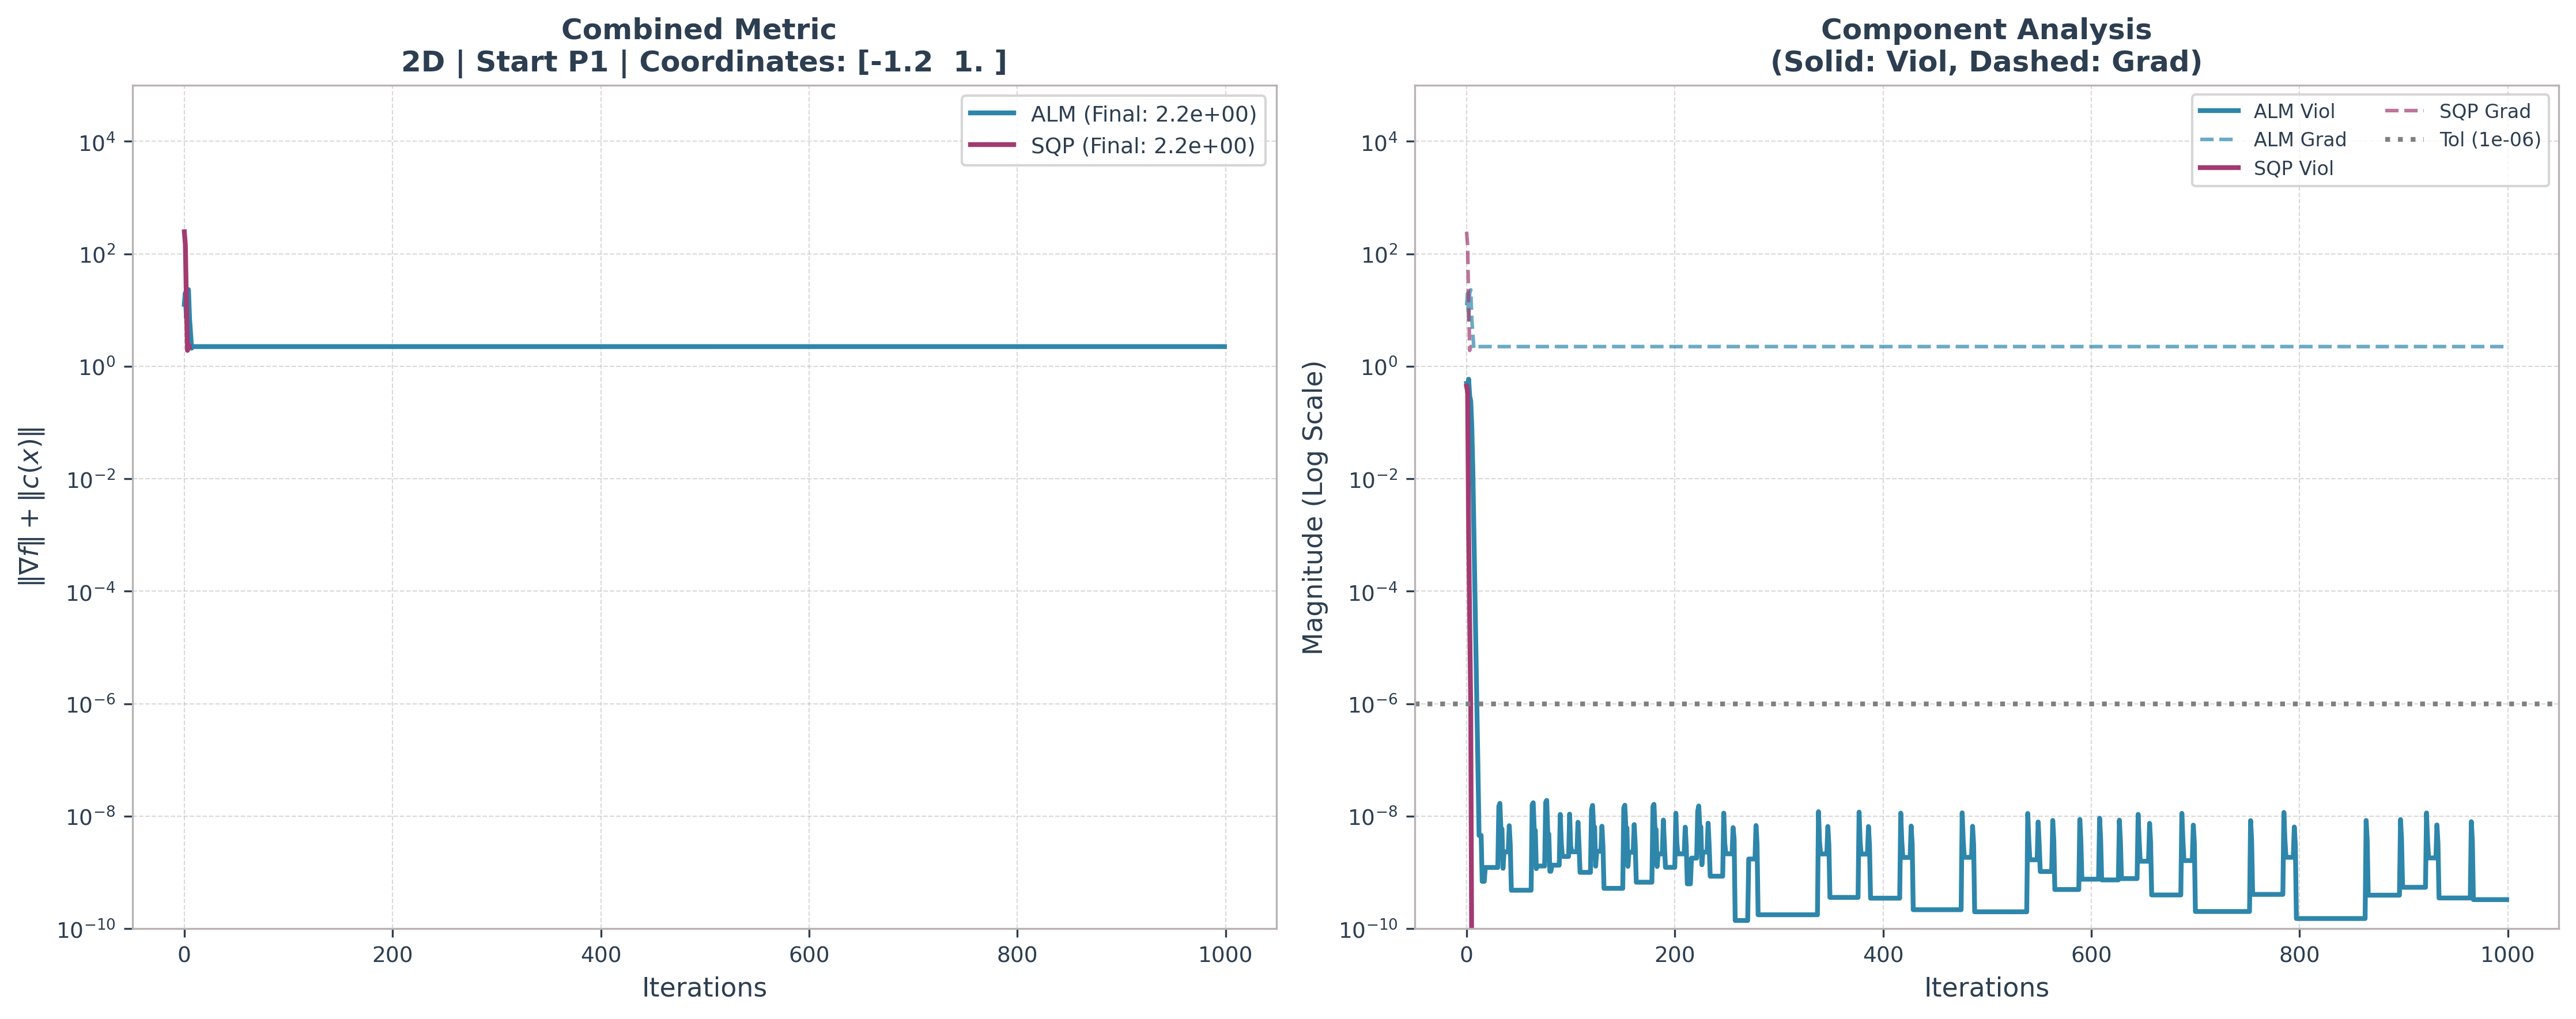
\includegraphics[width=1.0\textwidth]{figures/conv_dual_2D_P1.png}
        \caption{P1: Start $[-1.2, 1.]$}
    \end{subfigure}
    
    \vspace{1em} % 图片间距
    
    % P2
    \begin{subfigure}[b]{1.0\textwidth}
        \centering
        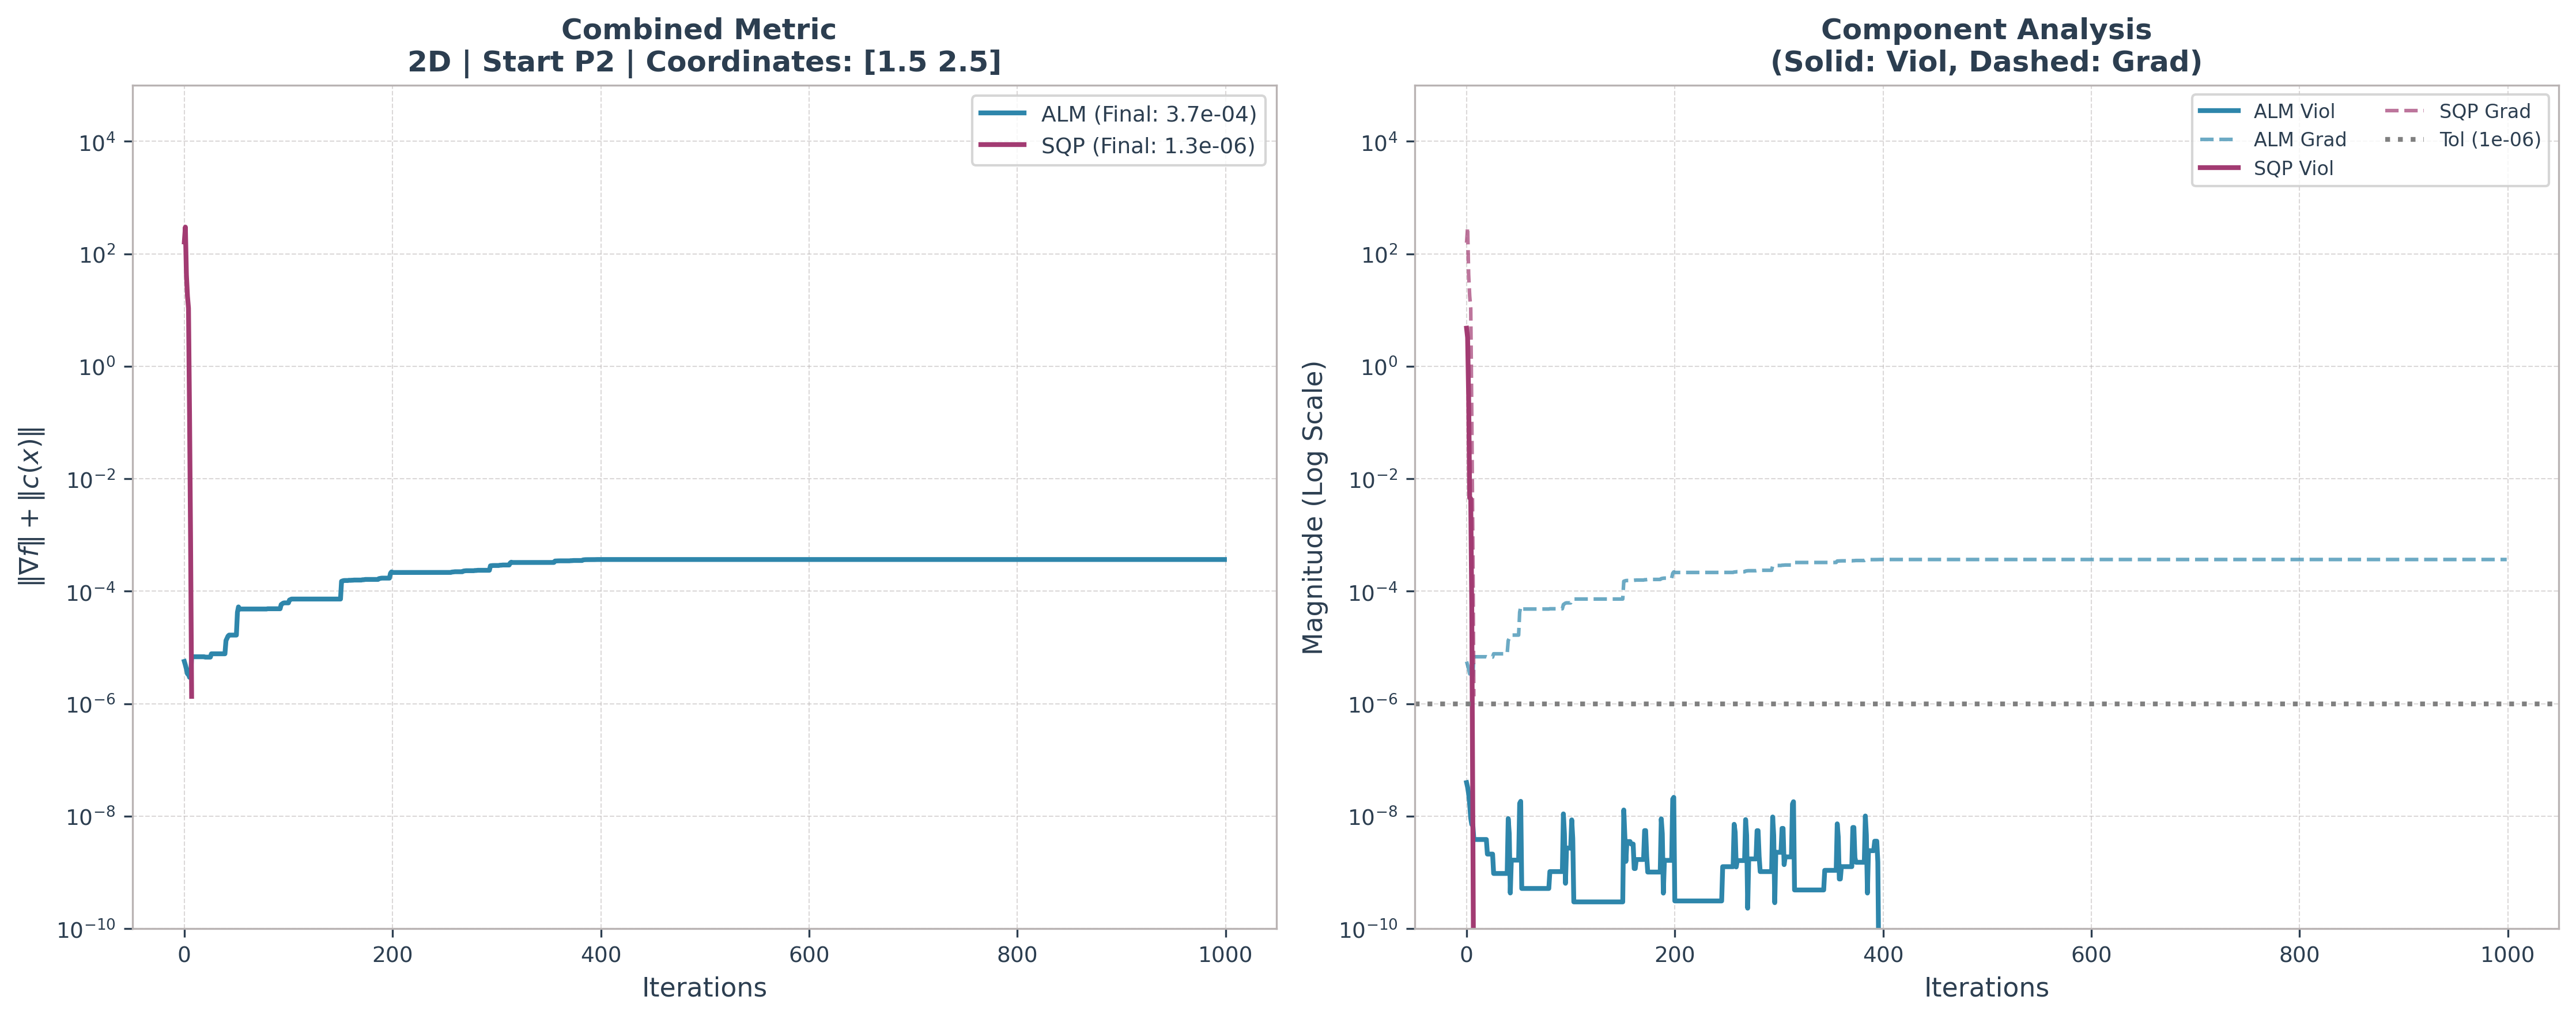
\includegraphics[width=1.0\textwidth]{figures/conv_dual_2D_P2.png}
        \caption{P2: Start $[1.5, 2.5]$}
    \end{subfigure}
    
    \caption{ALM与SQP算法在不同初始点下的收敛曲线对比（P1-P2）。左子图：综合KKT误差；右子图：误差分量分解（实线为约束违反度，虚线为梯度范数）。}
    \label{fig:2d_convergence}
\end{figure}

% --- 第二部分：包含 P3 和 P4 ---
\begin{figure}[H]
    \ContinuedFloat % 保持编号连续
    \centering
    % \addtocounter{subfigure}{2} # 无需增加计数器
    % P3
    \begin{subfigure}[b]{1.0\textwidth}
        \centering
        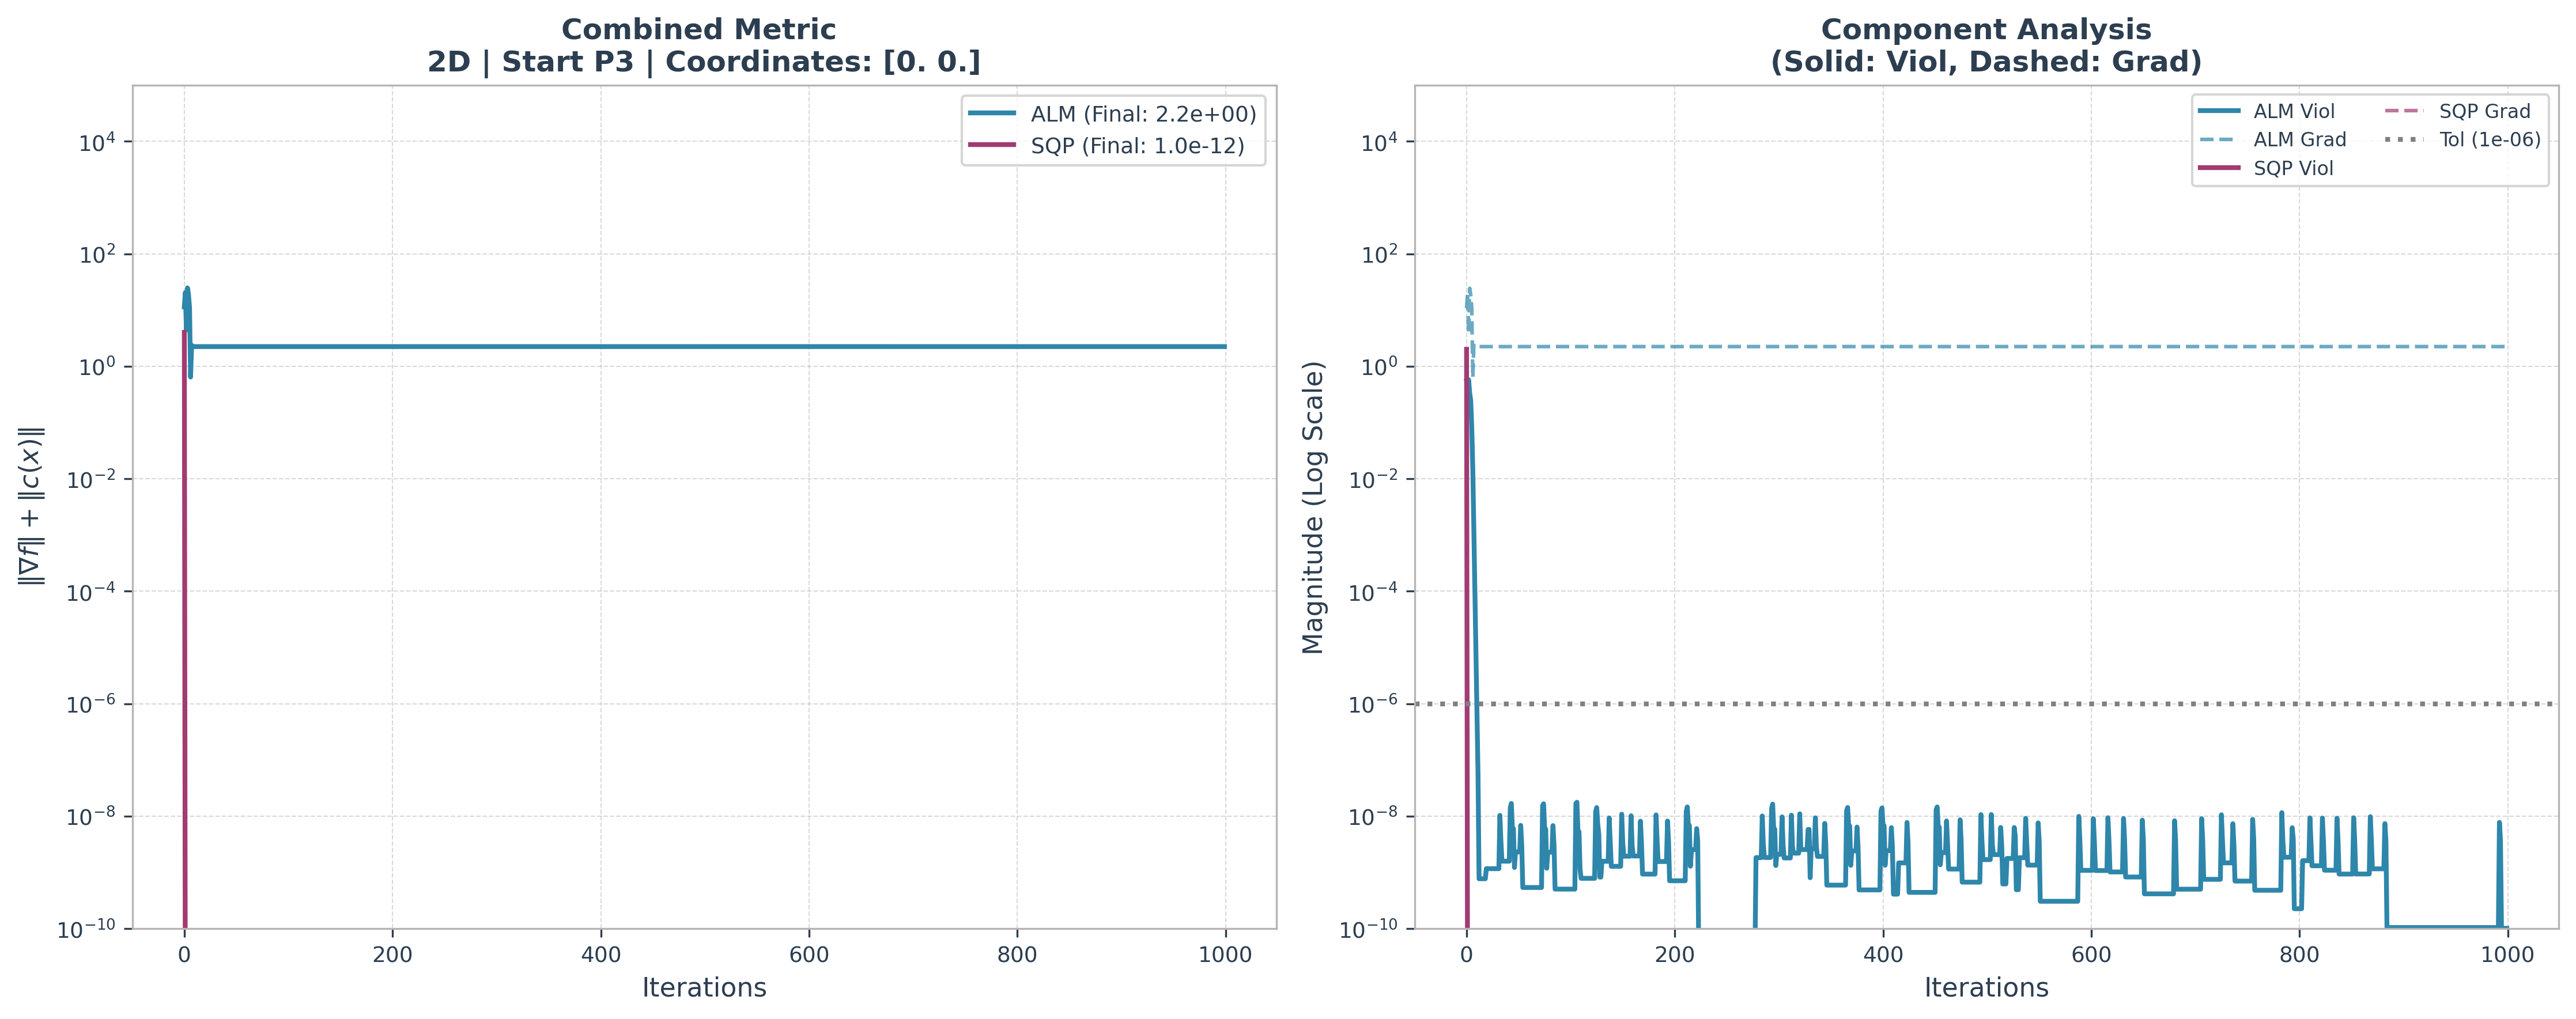
\includegraphics[width=1.0\textwidth]{figures/conv_dual_2D_P3.png}
        \caption{P3: Start $[0., 0.]$}
    \end{subfigure}
    
    \vspace{1em}
    
    % P4
    \begin{subfigure}[b]{1.0\textwidth}
        \centering
        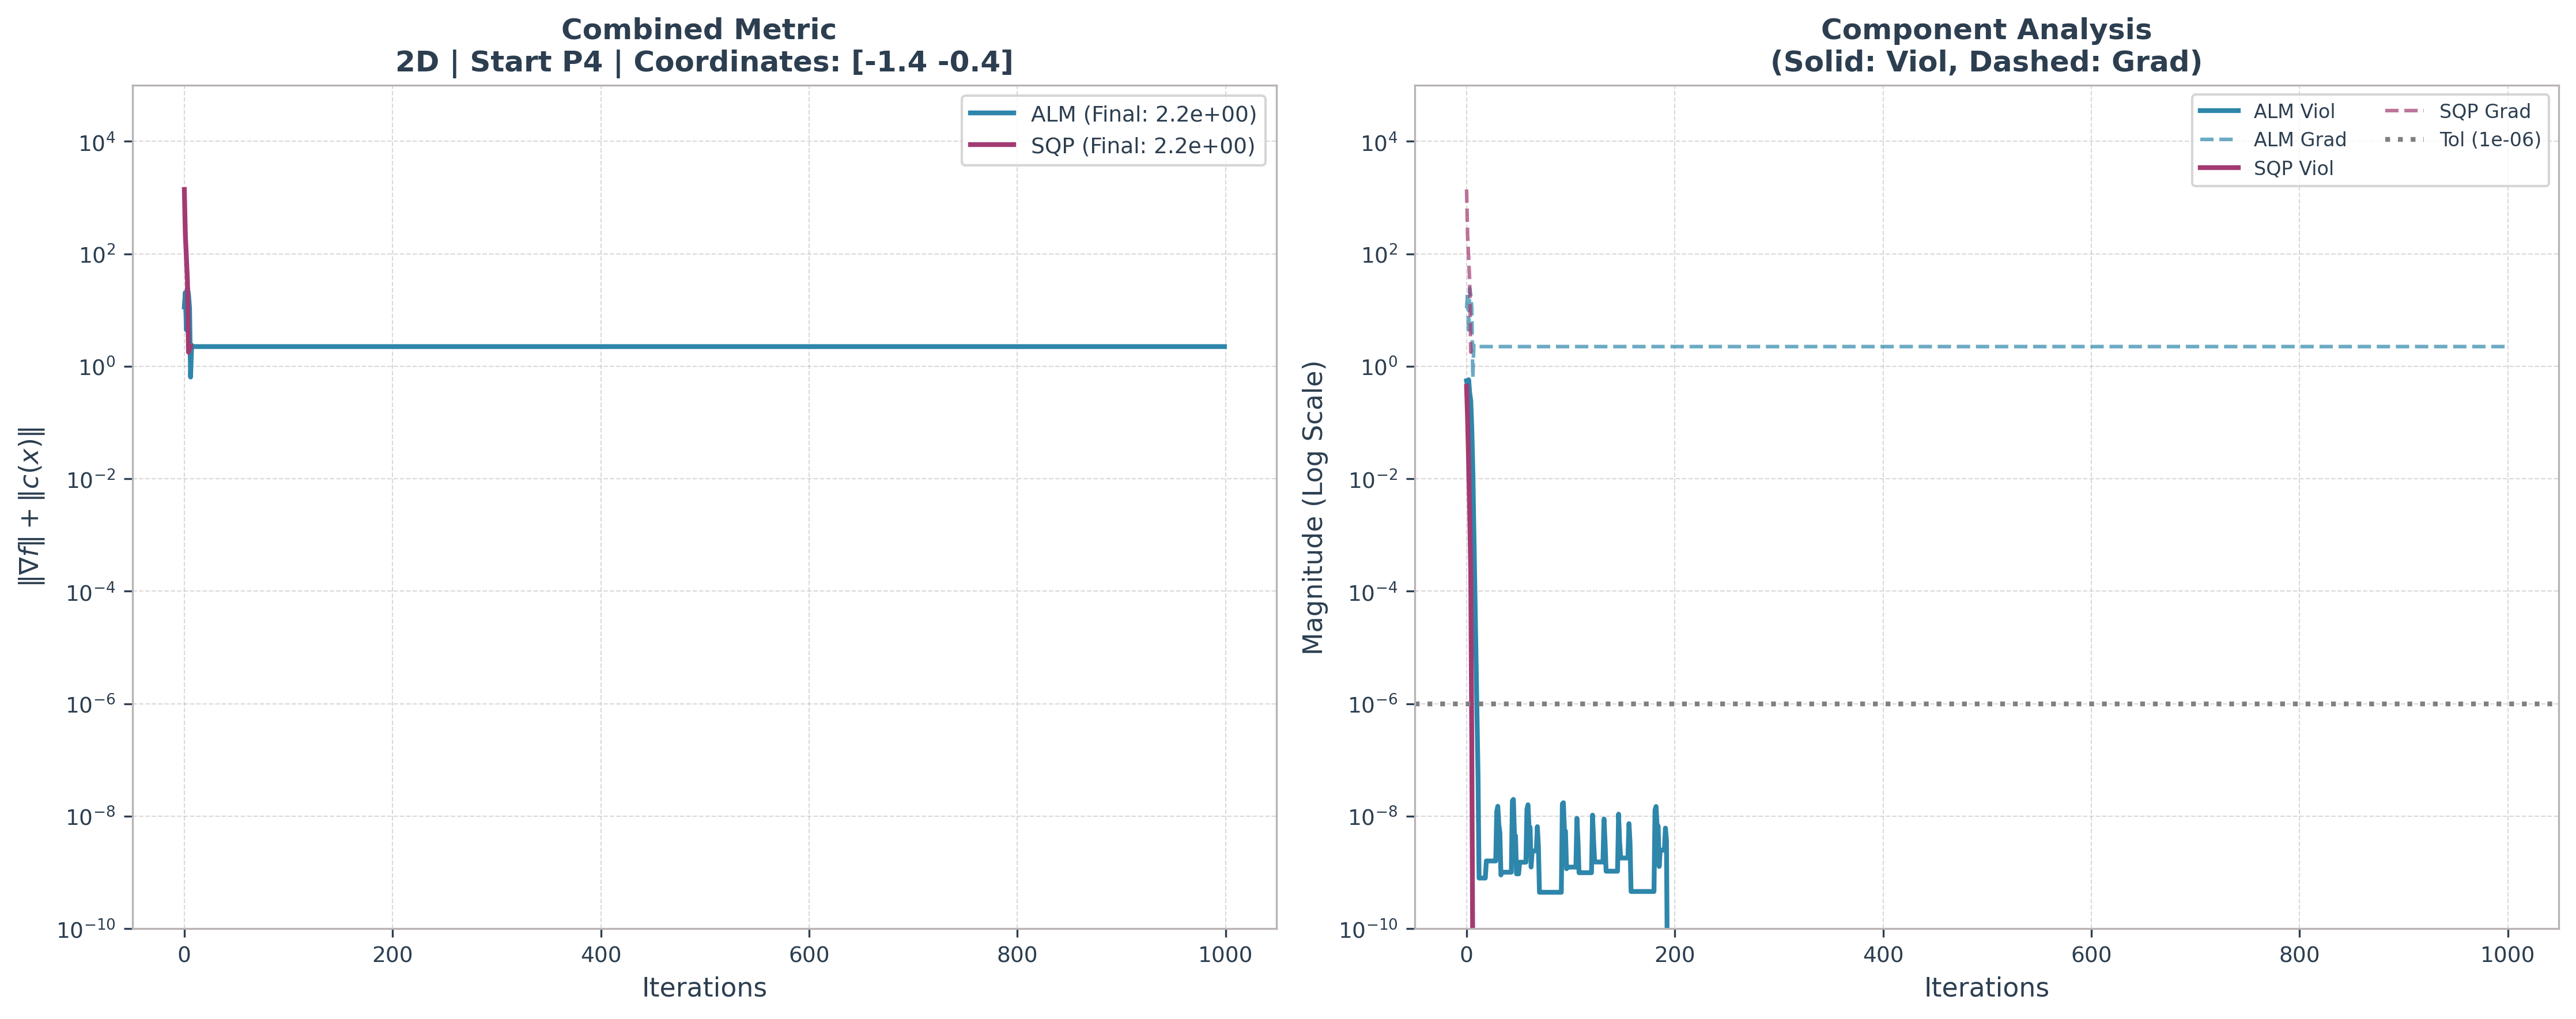
\includegraphics[width=1.0\textwidth]{figures/conv_dual_2D_P4.png}
        \caption{P4: Start $[-1.4, -0.4]$}
    \end{subfigure}
    
    \caption[]{ALM与SQP算法在不同初始点下的收敛曲线对比（续）。}
    \label{fig:2d_convergence_part2}
\end{figure}

% --- 第三部分：包含 P5 和 P6 ---
\begin{figure}[H]
    \ContinuedFloat % 保持编号连续
    \centering
    % \addtocounter{subfigure}{2} # 无需增加计数器
    % P5
    \begin{subfigure}[b]{1.0\textwidth}
        \centering
        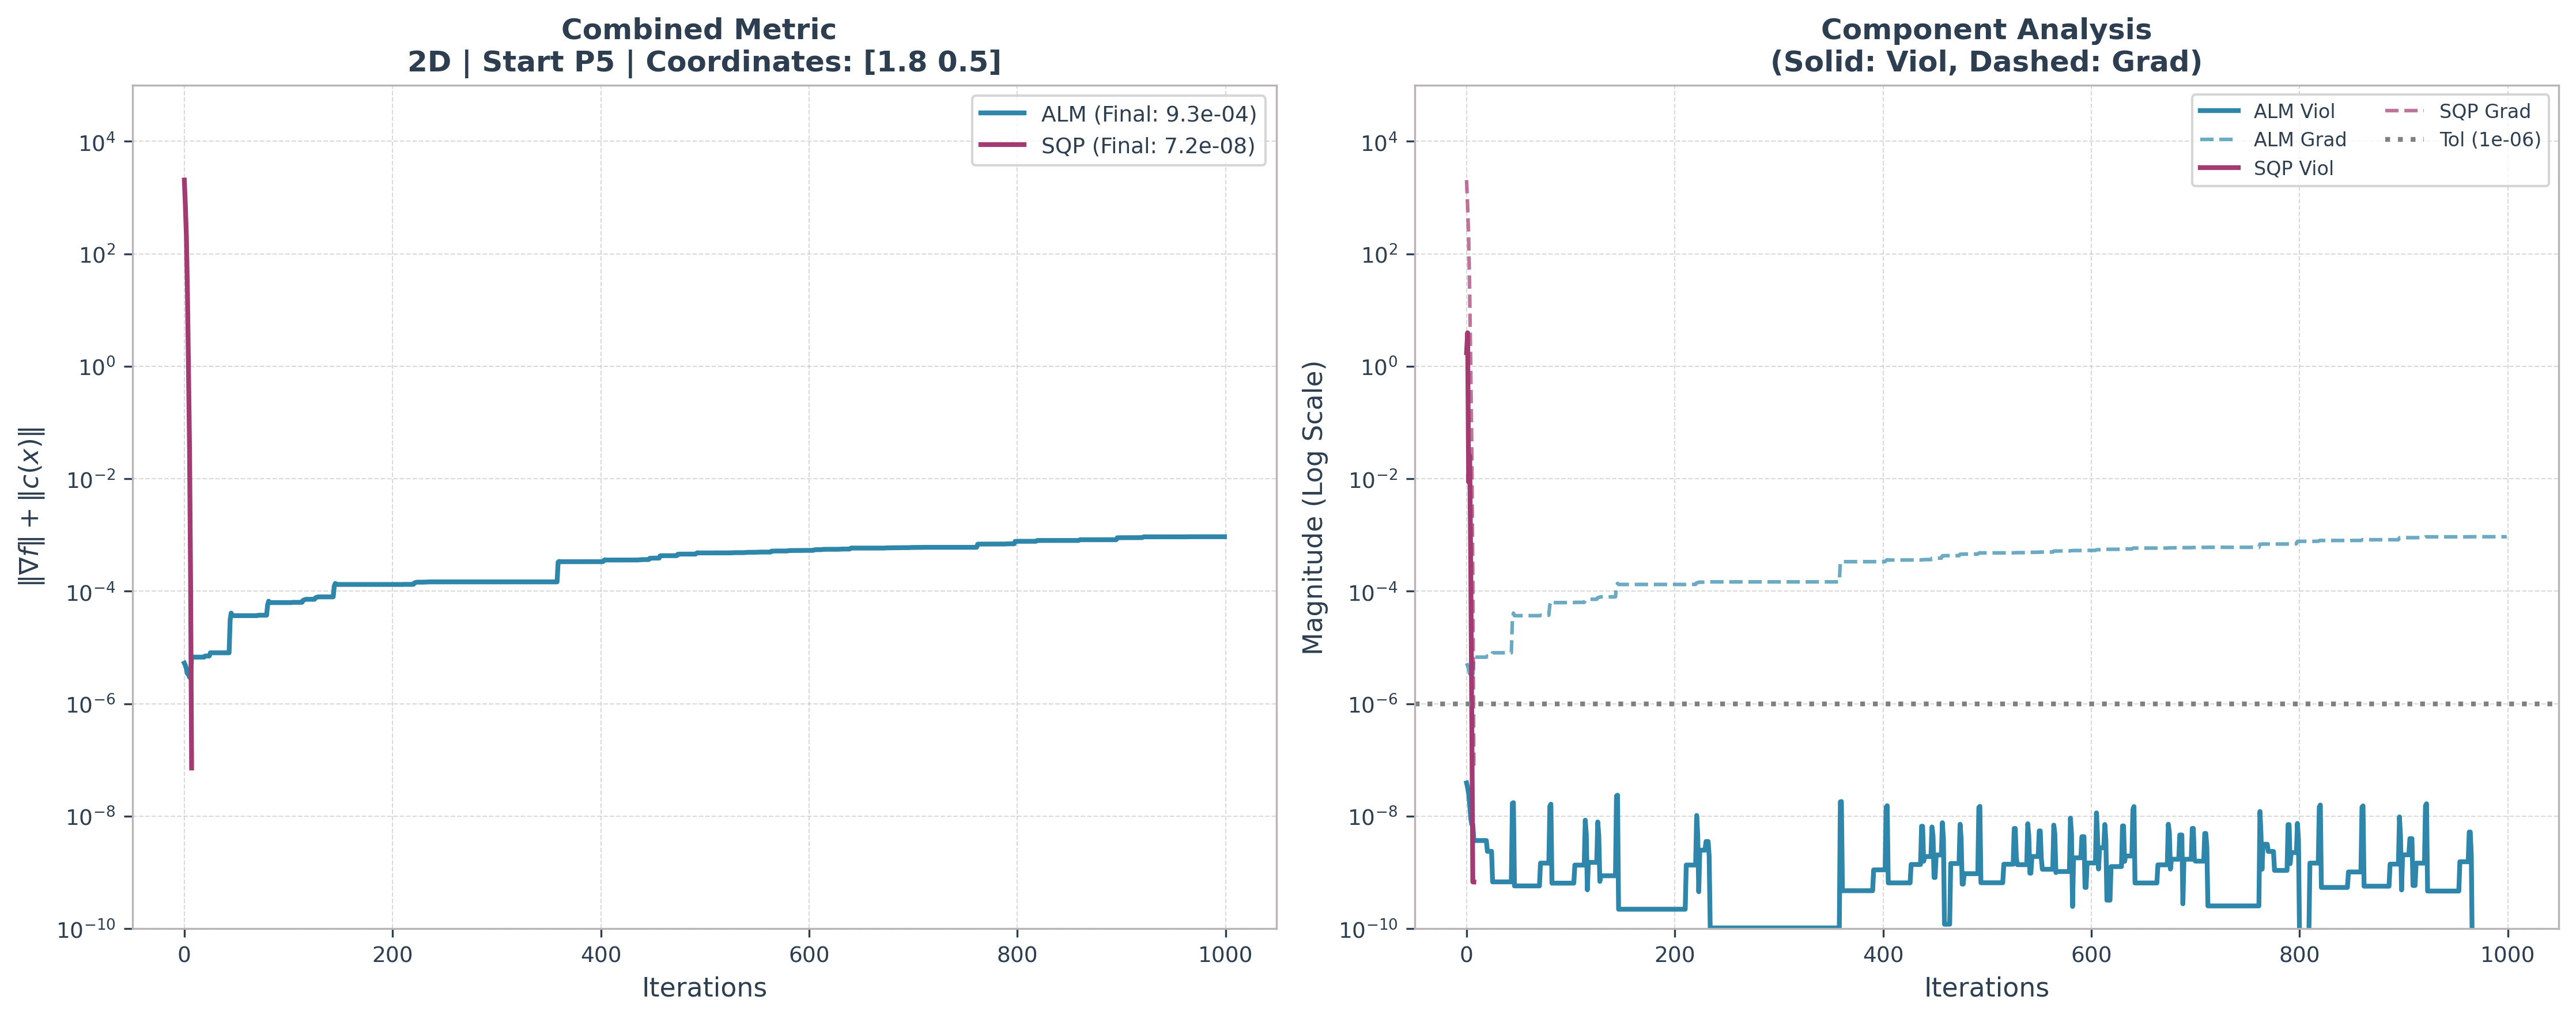
\includegraphics[width=1.0\textwidth]{figures/conv_dual_2D_P5.png}
        \caption{P5: Start $[1.8, 0.5]$}
    \end{subfigure}
    
    \vspace{1em}
    
    % P6
    \begin{subfigure}[b]{1.0\textwidth}
        \centering
        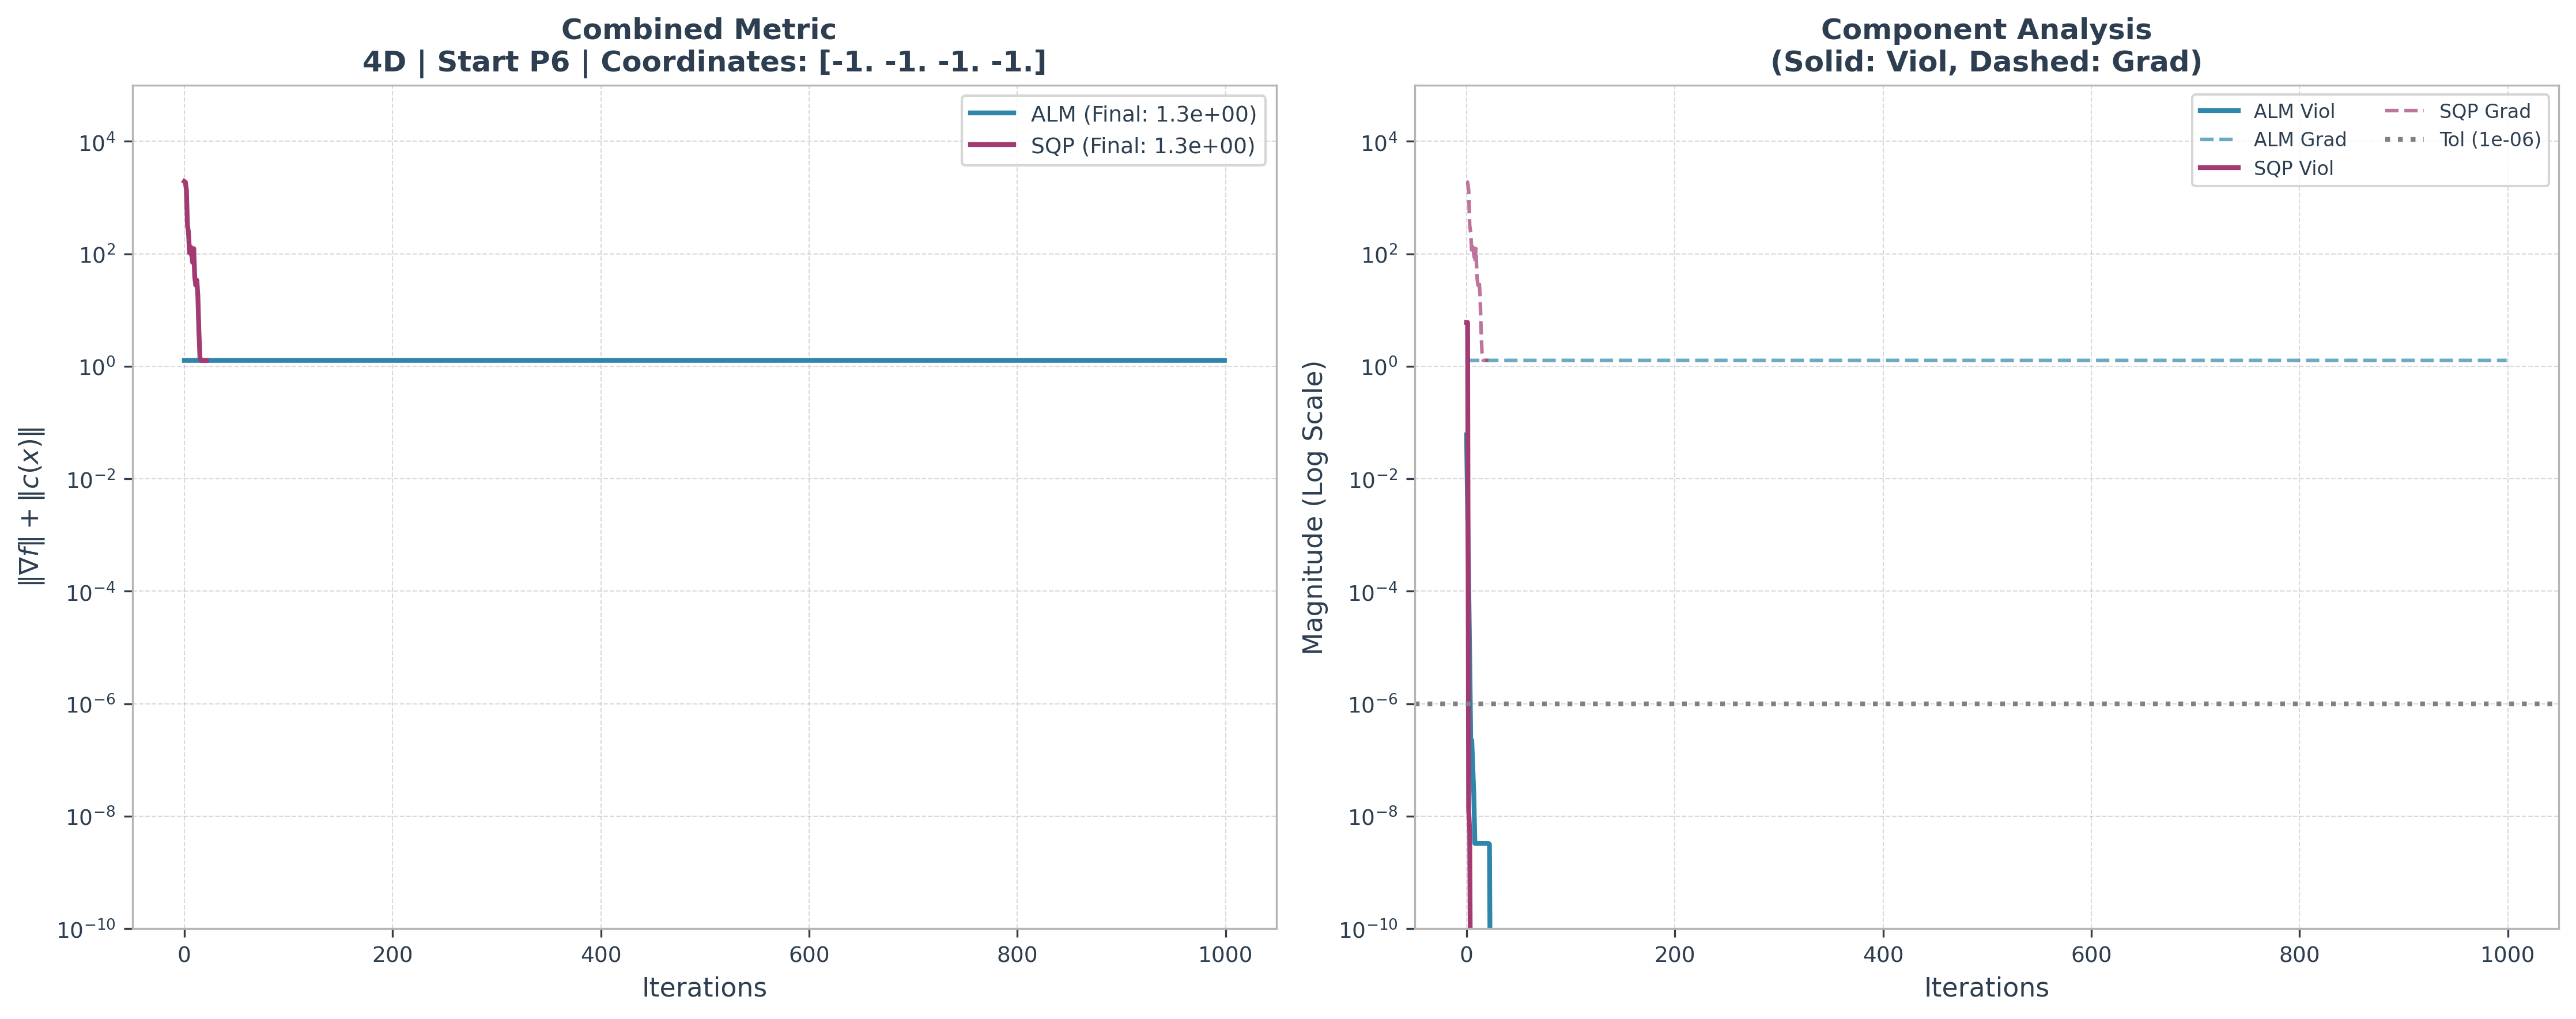
\includegraphics[width=1.0\textwidth]{figures/conv_dual_4D_P6.png}
        \caption{P6: Start $[0.5, 2.8]$}
    \end{subfigure}
    
    \caption[]{ALM与SQP算法在不同初始点下的收敛曲线对比（续）。}
    \label{fig:2d_convergence_part3}
\end{figure}




\paragraph{结果分析：} 

\begin{enumerate}
    \item \textbf{全局最优与局部最优的吸引域差异}：
    观察初始点 P2 $[1.5, 2.5]$ 与 P1 $[-1.2, 1.0]$，两种算法均能成功收敛至满足 KKT 条件的稳定点。
    \begin{itemize}
        \item 对于 P2，ALM 和 SQP 均收敛至全局最优解，且 SQP 表现出特征性的二阶收敛速率，KKT 误差在最后几次迭代中呈现陡峭下降。
        \item 对于 P1 和 P4，由于目标函数的非凸性，算法受限于初始点所在的吸引域，收敛至局部最优解。这表明在非凸优化问题中，算法的最终解高度依赖于初始值的选取。
    \end{itemize}

    \item \textbf{特殊点的分支行为}：
    初始点 P3 $[0, 0]$ 展示了一个典型的分叉现象。该点位于目标函数几何结构的鞍点或不同吸引域的边界附近。ALM 与 SQP 由于搜索方向（分别为梯度下降方向与牛顿方向）及步长策略的差异，导致迭代轨迹分别滑向了不同的极值点。这一现象验证了不同算法对临界点敏感度的差异。

    \item \textbf{收敛机制的对比}：
    \begin{itemize}
        \item \textbf{SQP 算法}：在所有测试点中，SQP 算法一旦进入信任域或线搜索满足下降条件的区域，其误差曲线（特别是右子图中的虚线，即梯度范数）通常呈现单调且快速的下降。这符合牛顿法在解邻域内具备二次收敛性的理论预期。
        \item \textbf{ALM 算法}：从右子图的实线（约束违反度）可以看出，ALM 的收敛过程呈现出明显的阶段性特征。在罚参数 $\mu$ 更新的初期，算法主要致力于最小化增广拉格朗日函数，允许一定的约束违反；随着外层循环增加 $\mu$ 值，约束违反度被迫下降。这种“先优化后可行”的策略使得其收敛曲线呈现阶梯状，收敛速度在迭代初期通常慢于 SQP。
    \end{itemize}
\end{enumerate}



\subsubsection{优化路径分析}

为了深入探究算法的寻优逻辑，我们将迭代路径叠加在目标函数的等高线图上，如图 \ref{fig:traj_analysis} 所示。

\begin{figure}[H]
    \centering
    % 第一行
    \begin{subfigure}{0.49\textwidth}
        \centering
        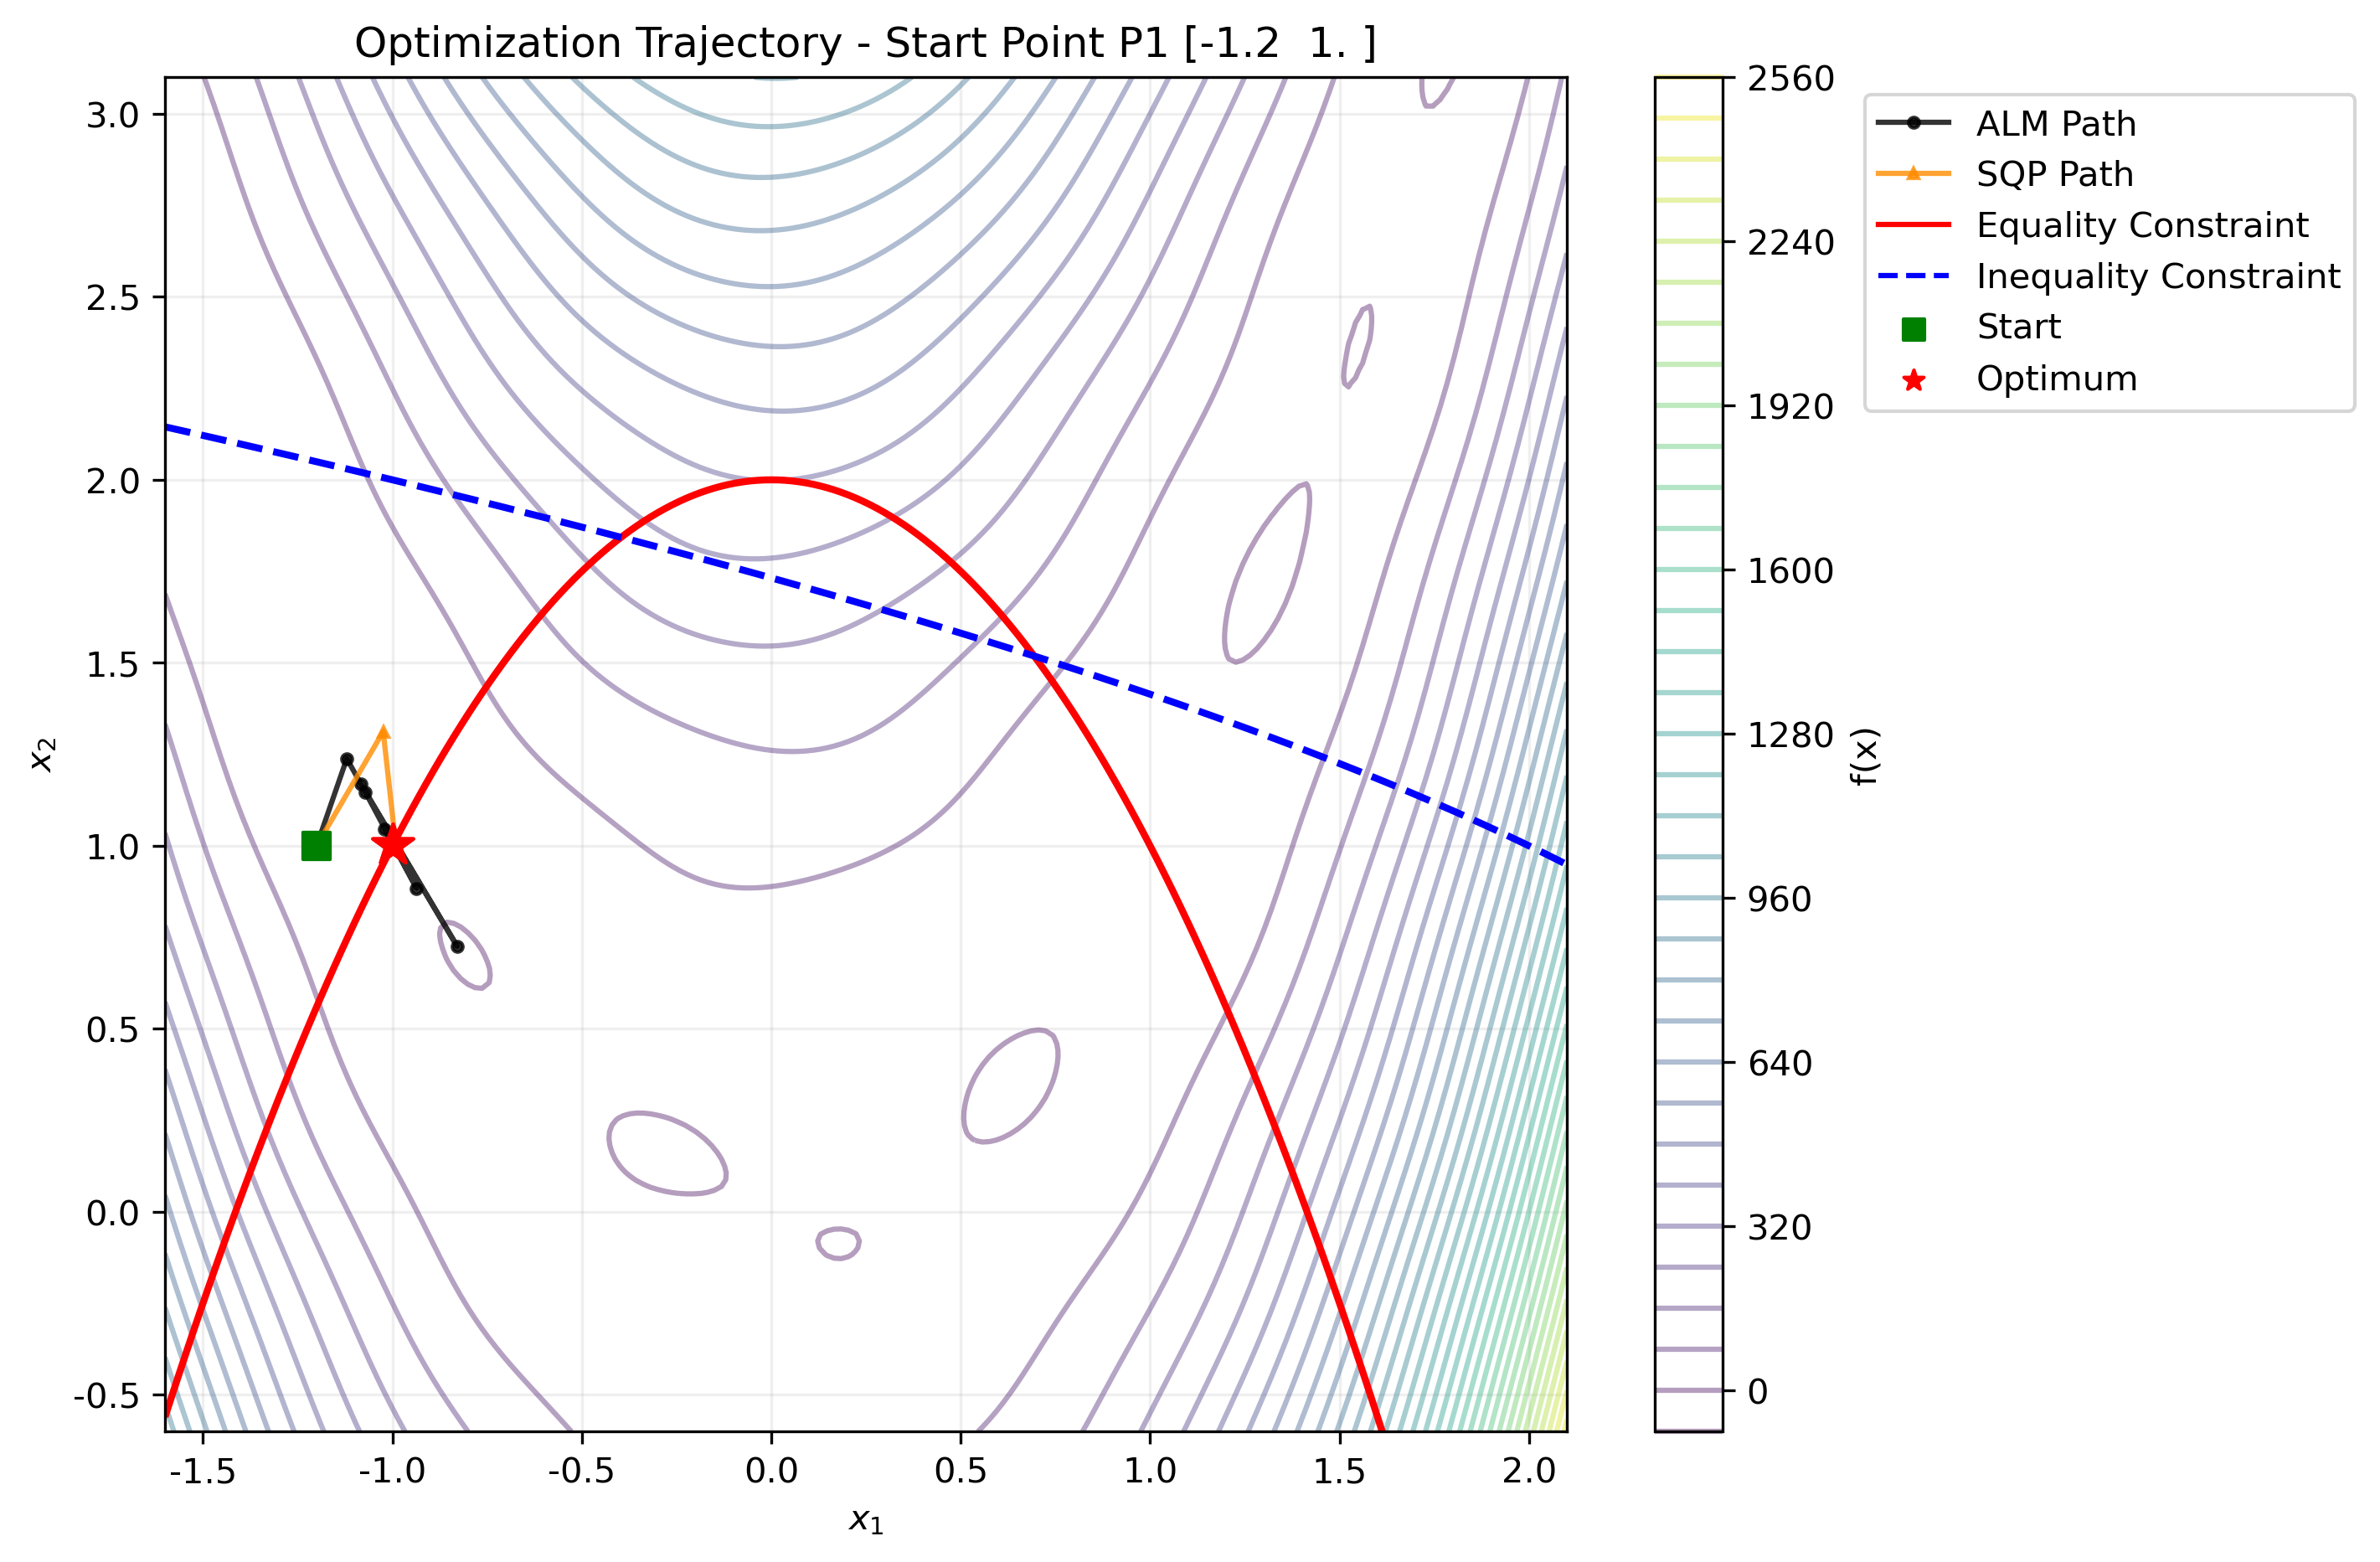
\includegraphics[width=\linewidth]{figures/path_2D_P1.png}
        \caption{P1: Start $[-1.2, 1.]$ (局部极小)}
        \label{subfig:p1}
    \end{subfigure}
    \hfill
    \begin{subfigure}{0.49\textwidth}
        \centering
        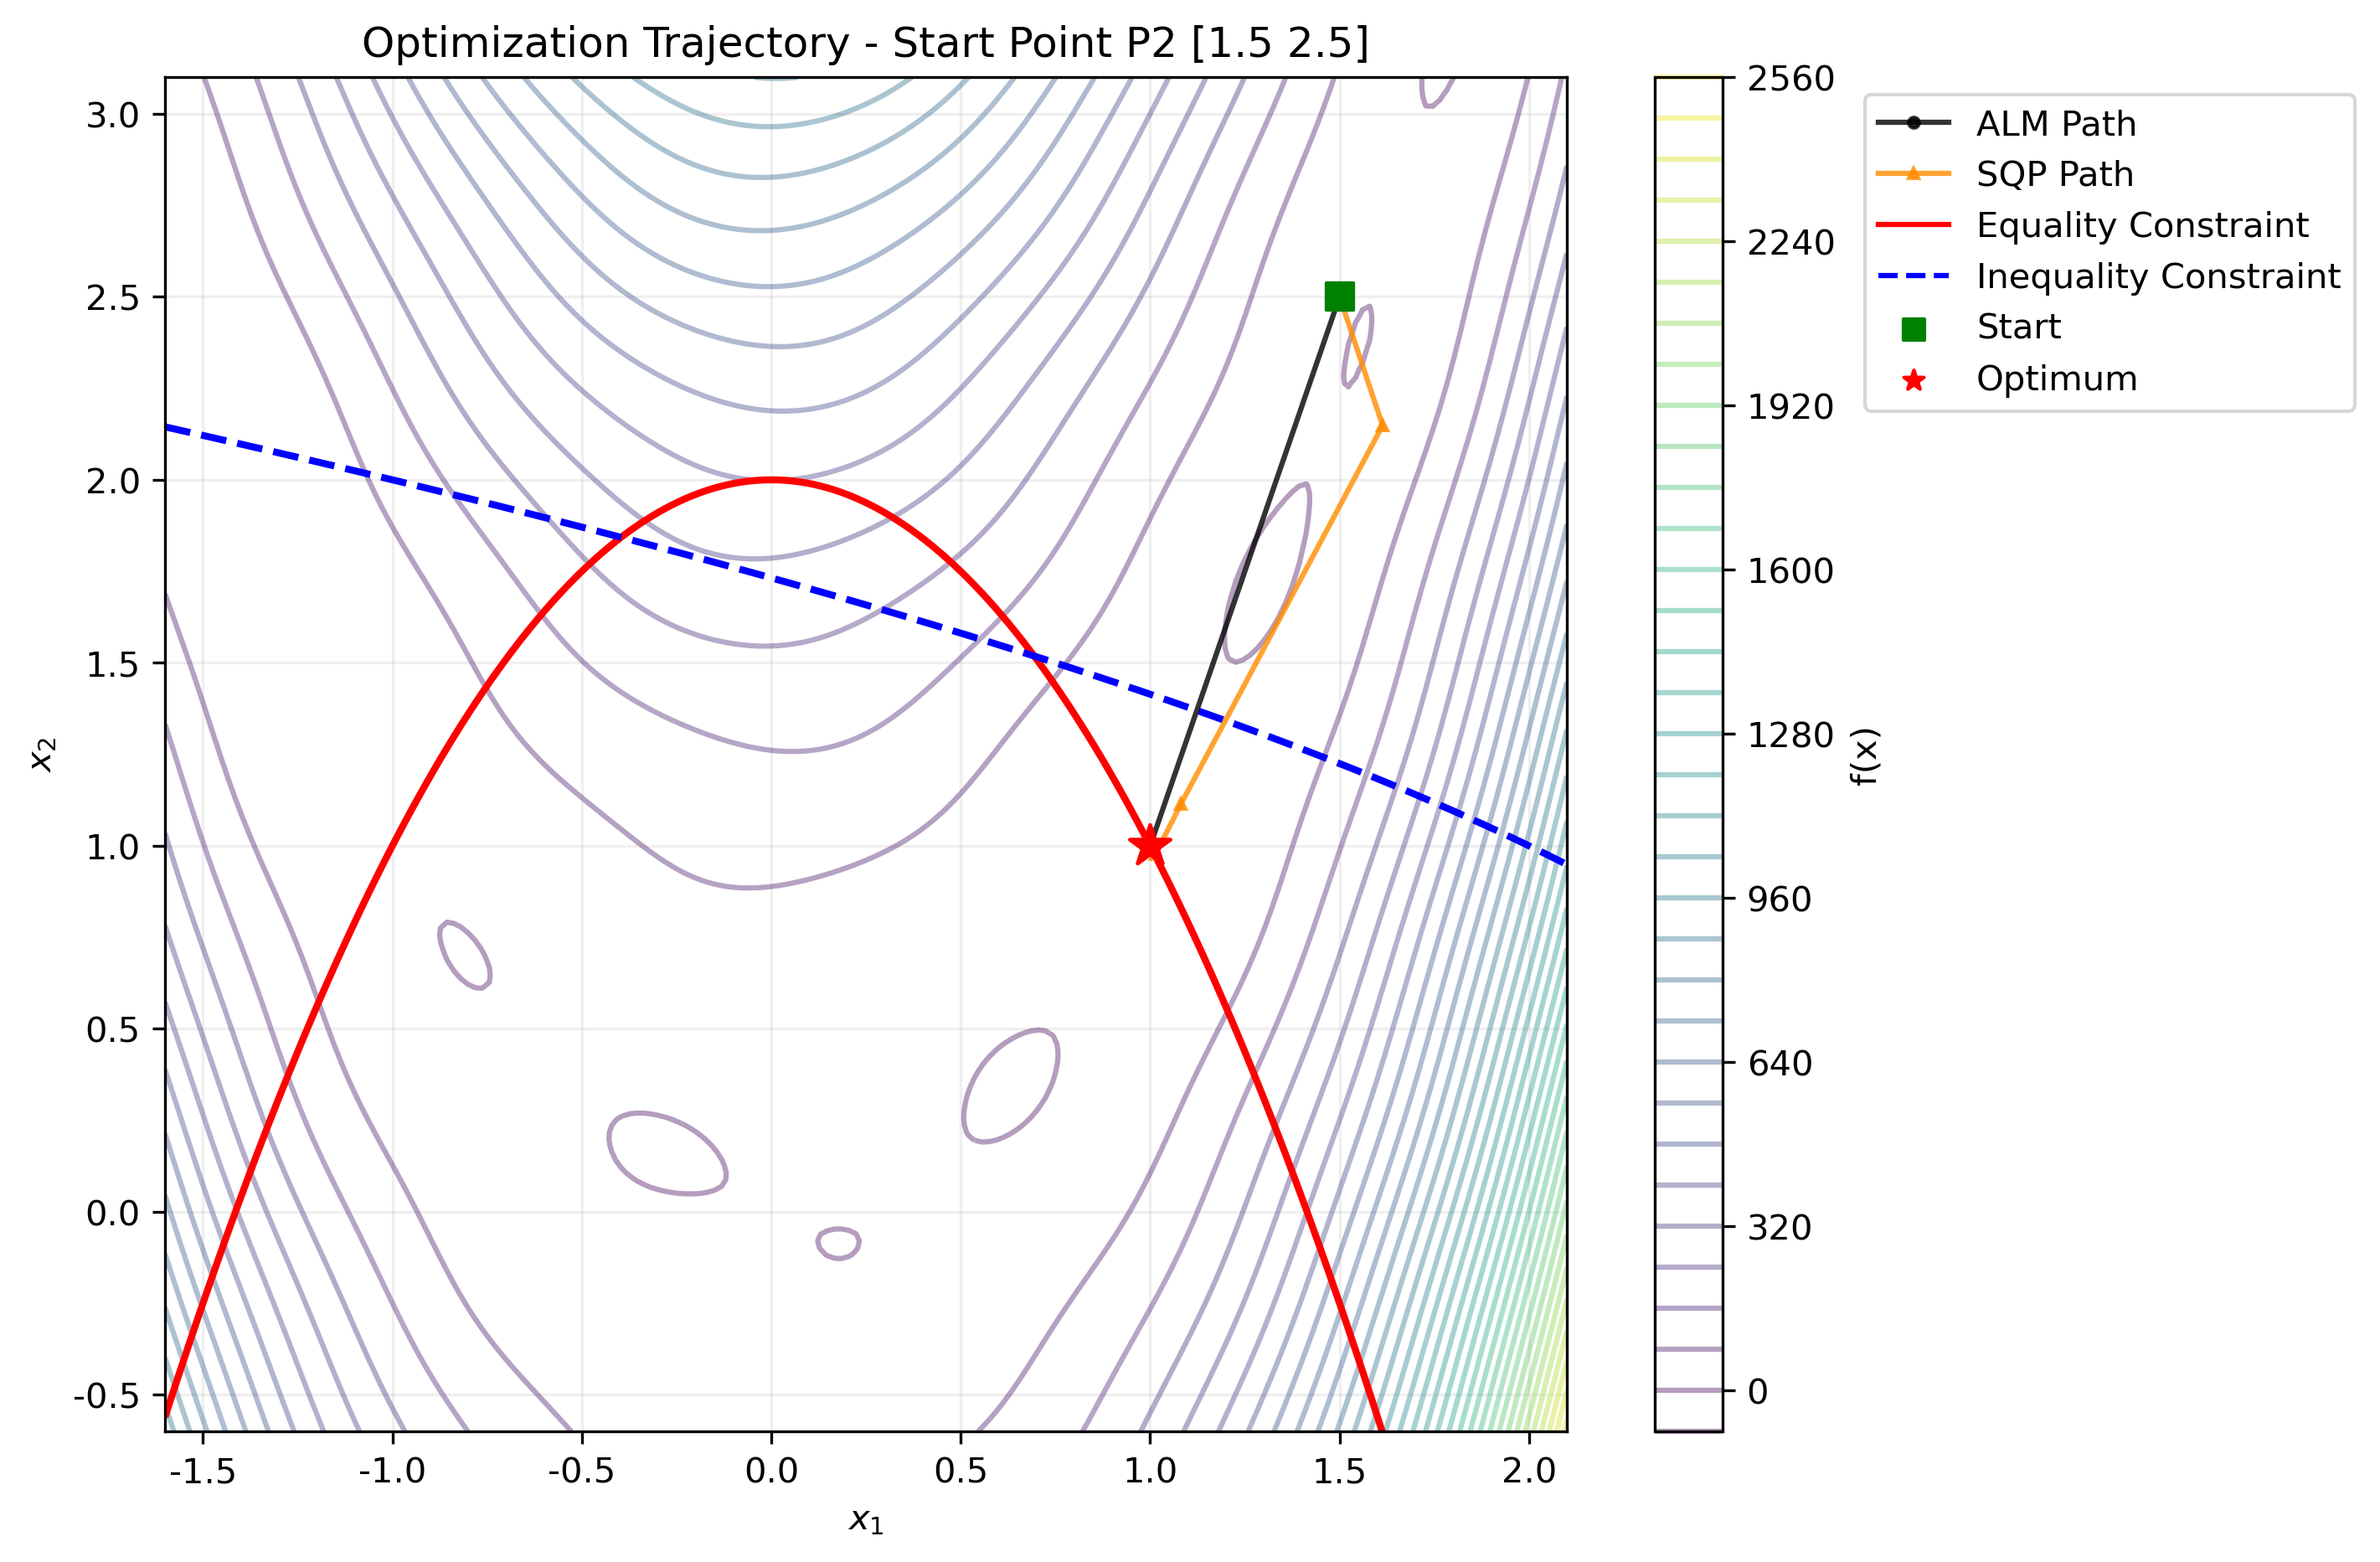
\includegraphics[width=\linewidth]{figures/path_2D_P2.png}
        \caption{P2: Start $[1.5, 2.5]$ (全局最优)}
        \label{subfig:p2}
    \end{subfigure}
    
    \vspace{0.8em} % 调整行间距
    
    % 第二行
    \begin{subfigure}{0.49\textwidth}
        \centering
        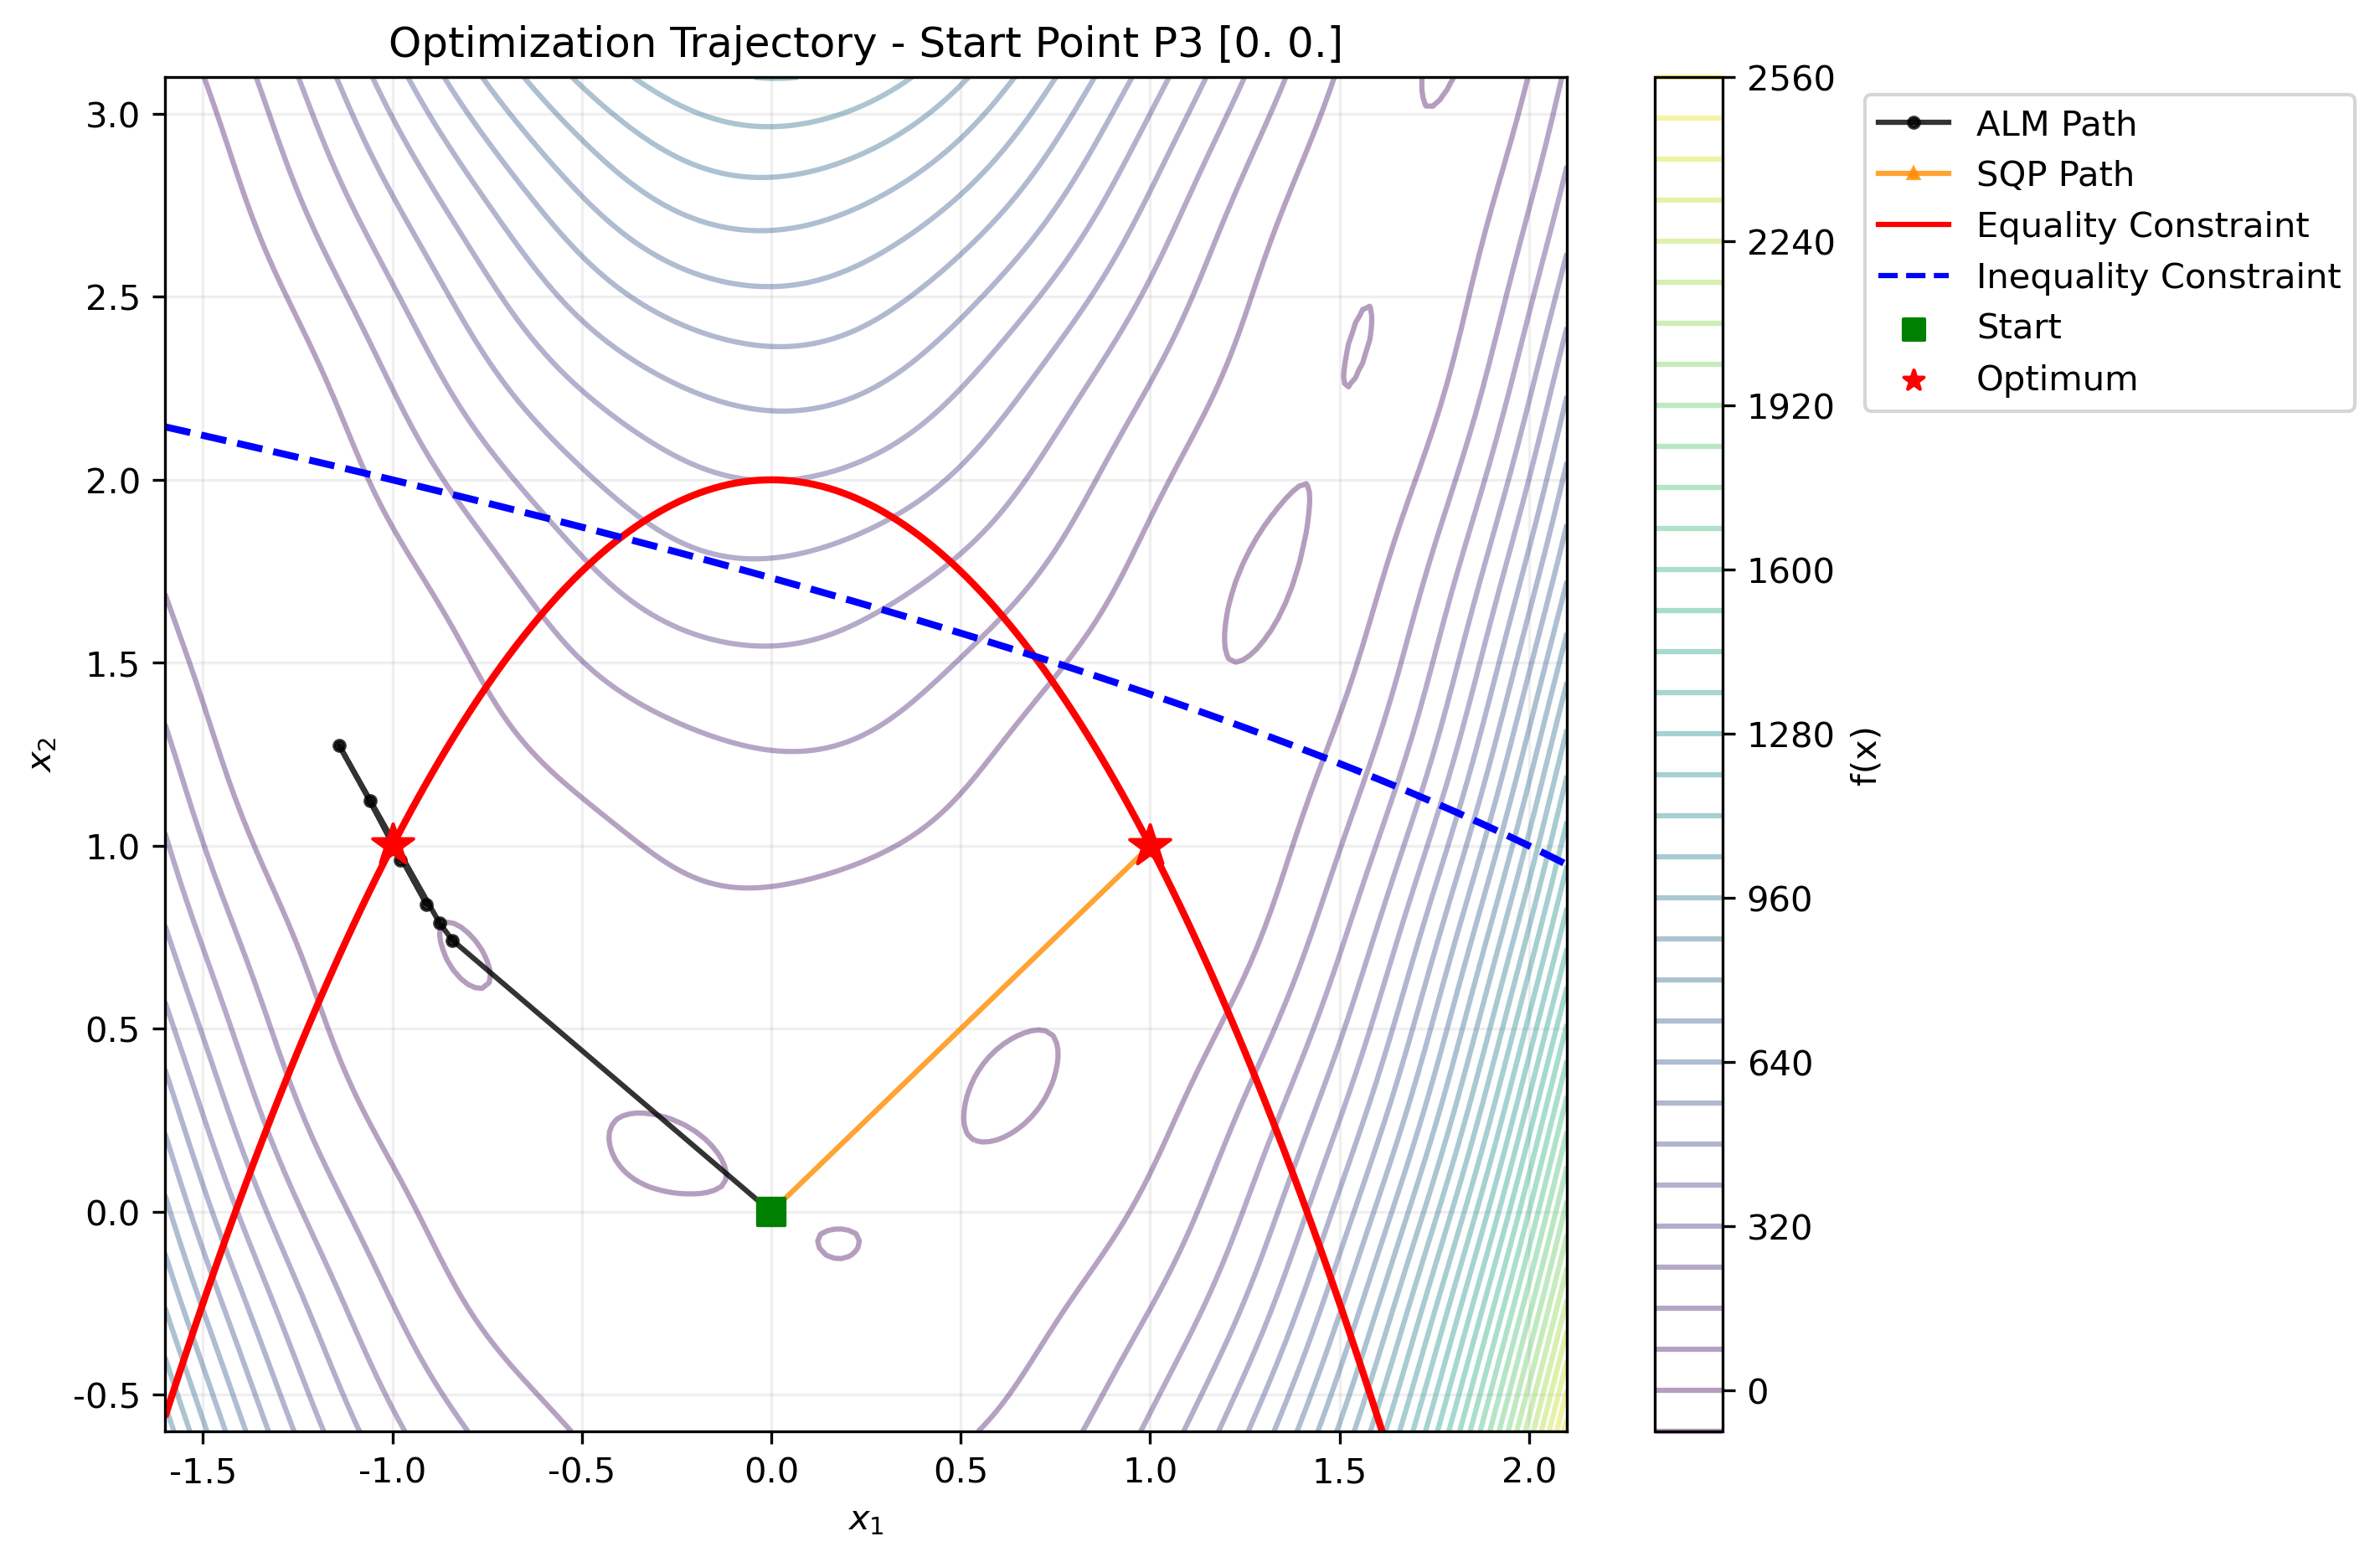
\includegraphics[width=\linewidth]{figures/path_2D_P3.png}
        \caption{P3: Start $[0., 0.]$ (算法分歧点)}
        \label{subfig:p3}
    \end{subfigure}
    \hfill
    \begin{subfigure}{0.49\textwidth}
        \centering
        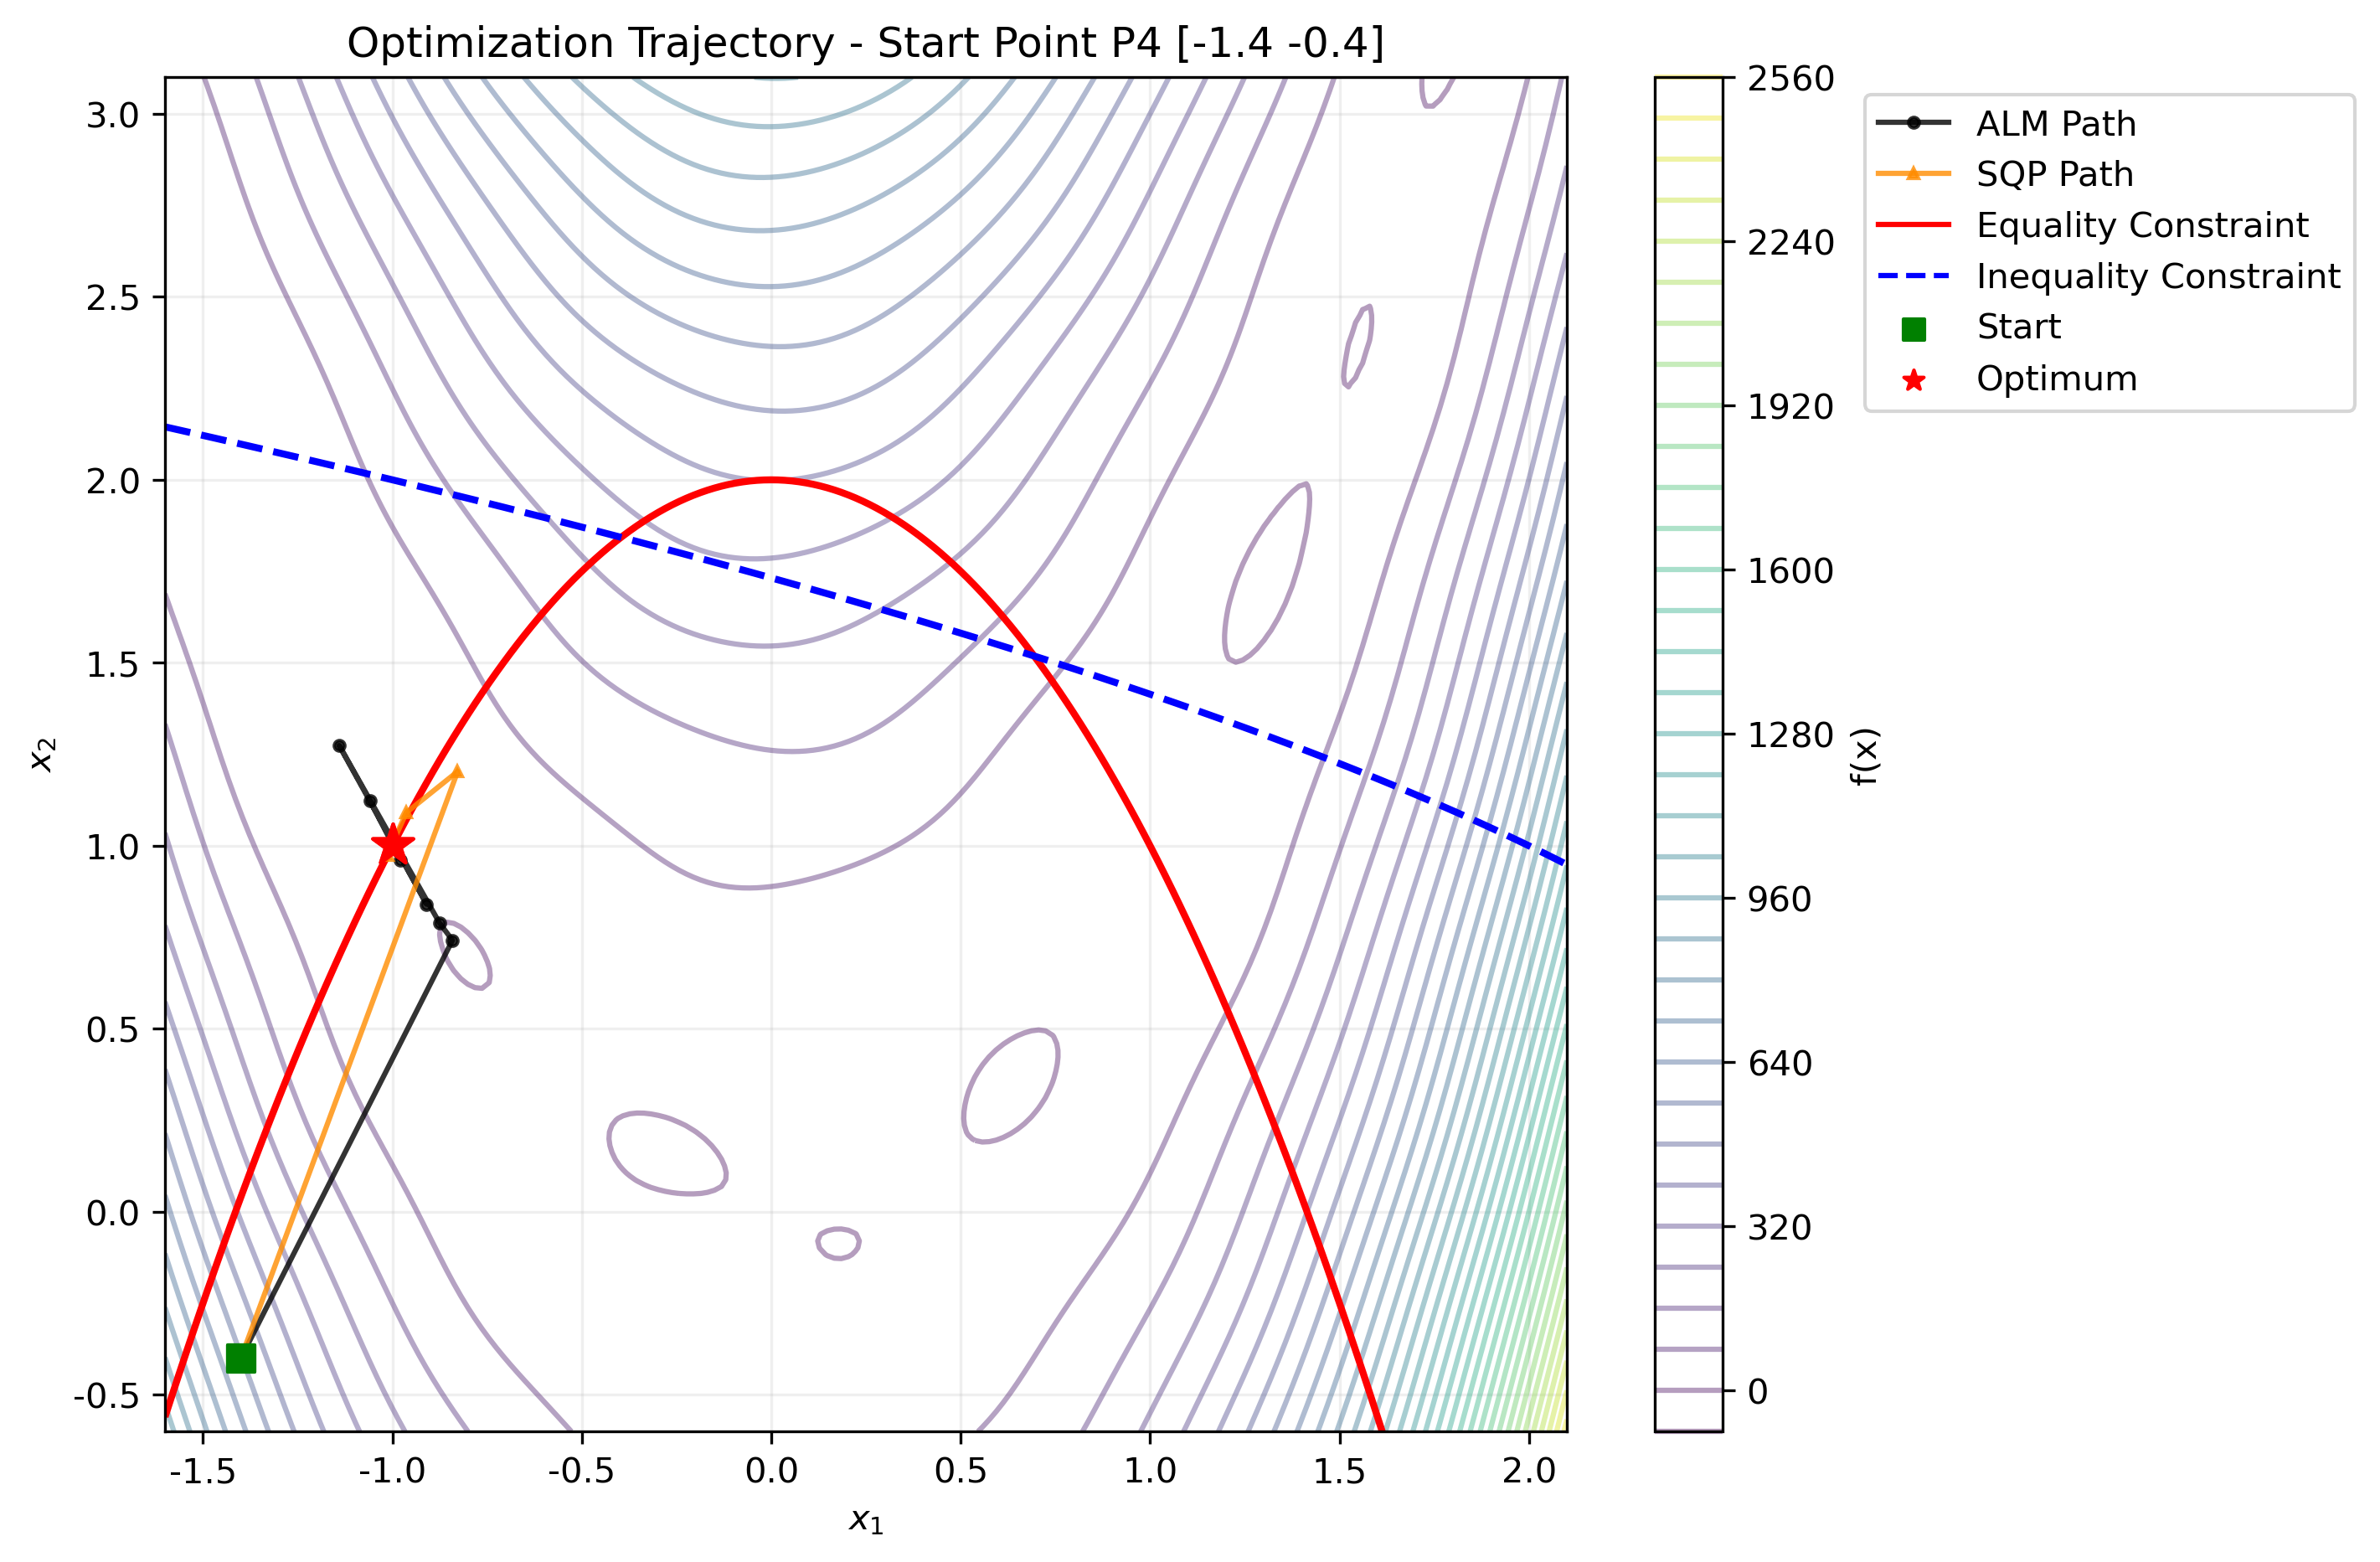
\includegraphics[width=\linewidth]{figures/path_2D_P4.png}
        \caption{P4: Start $[-1.4, -0.4]$ (局部极小)}
        \label{subfig:p4}
    \end{subfigure}
    
    \vspace{0.8em}
    
    % 第三行
    \begin{subfigure}{0.49\textwidth}
        \centering
        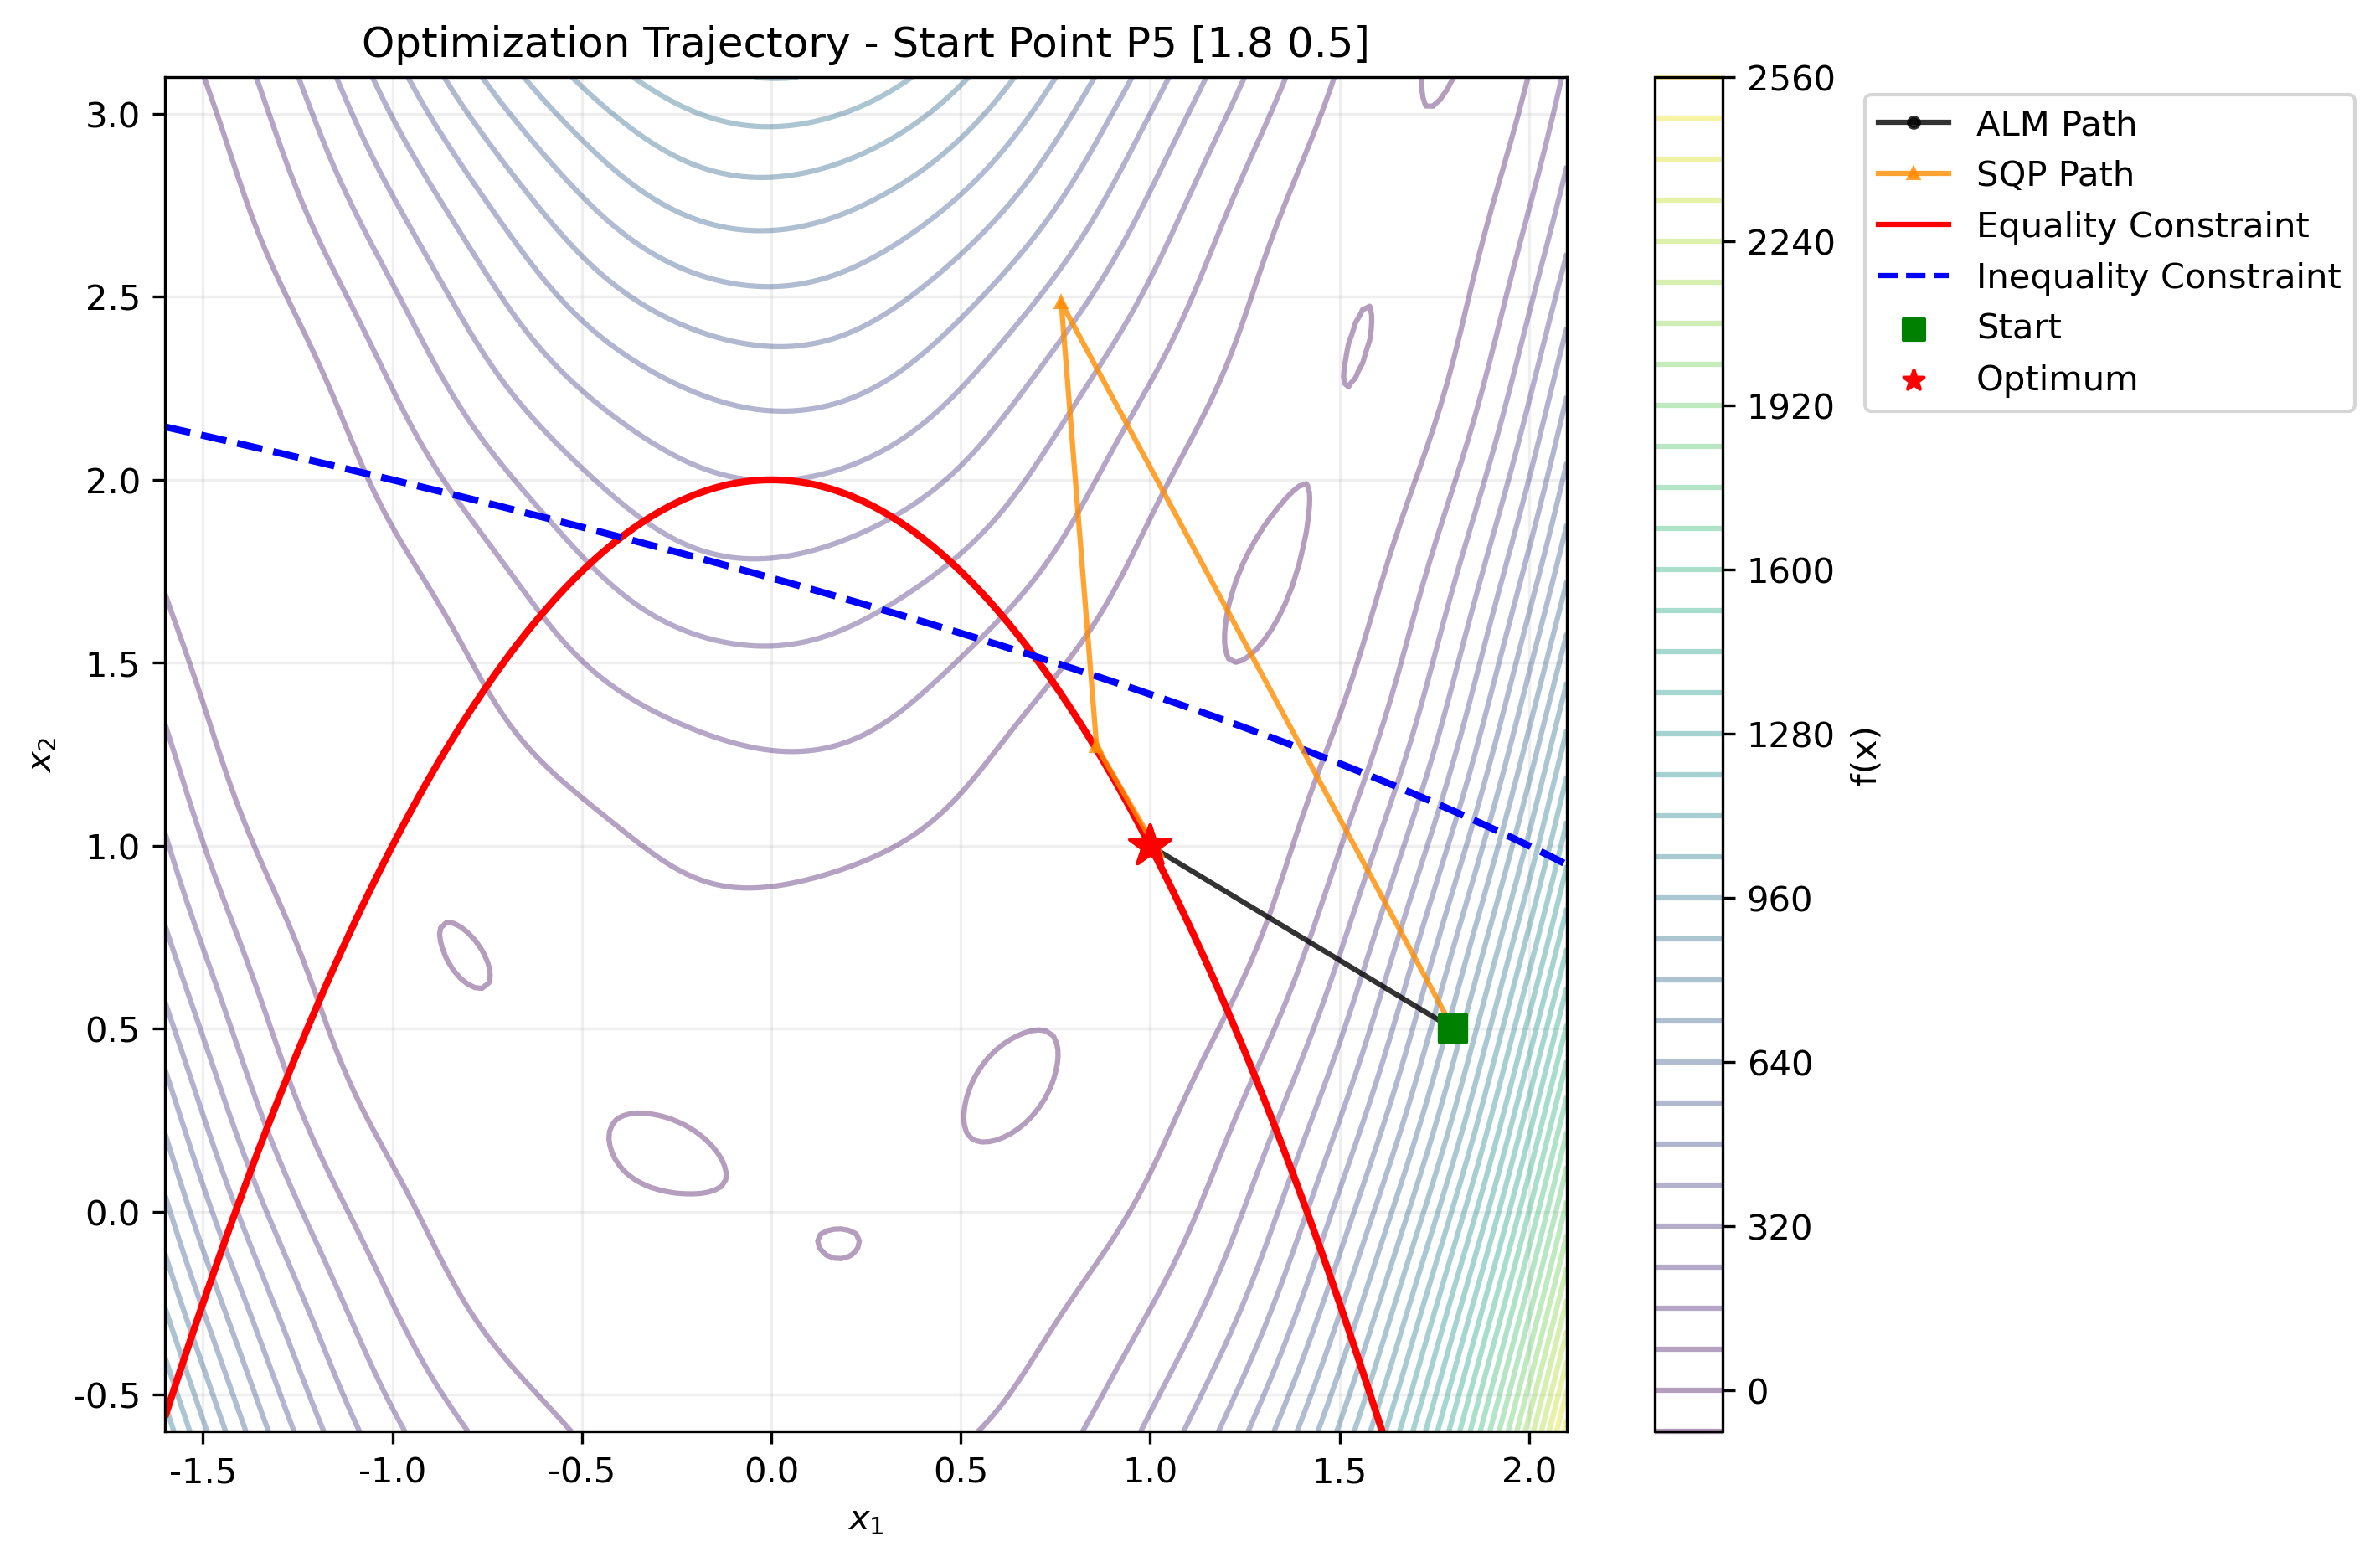
\includegraphics[width=\linewidth]{figures/path_2D_P5.png}
        \caption{P5: Start $[1.8, 0.5]$ (远端收敛)}
        \label{subfig:p5}
    \end{subfigure}
    \hfill
    \begin{subfigure}{0.49\textwidth}
        \centering
        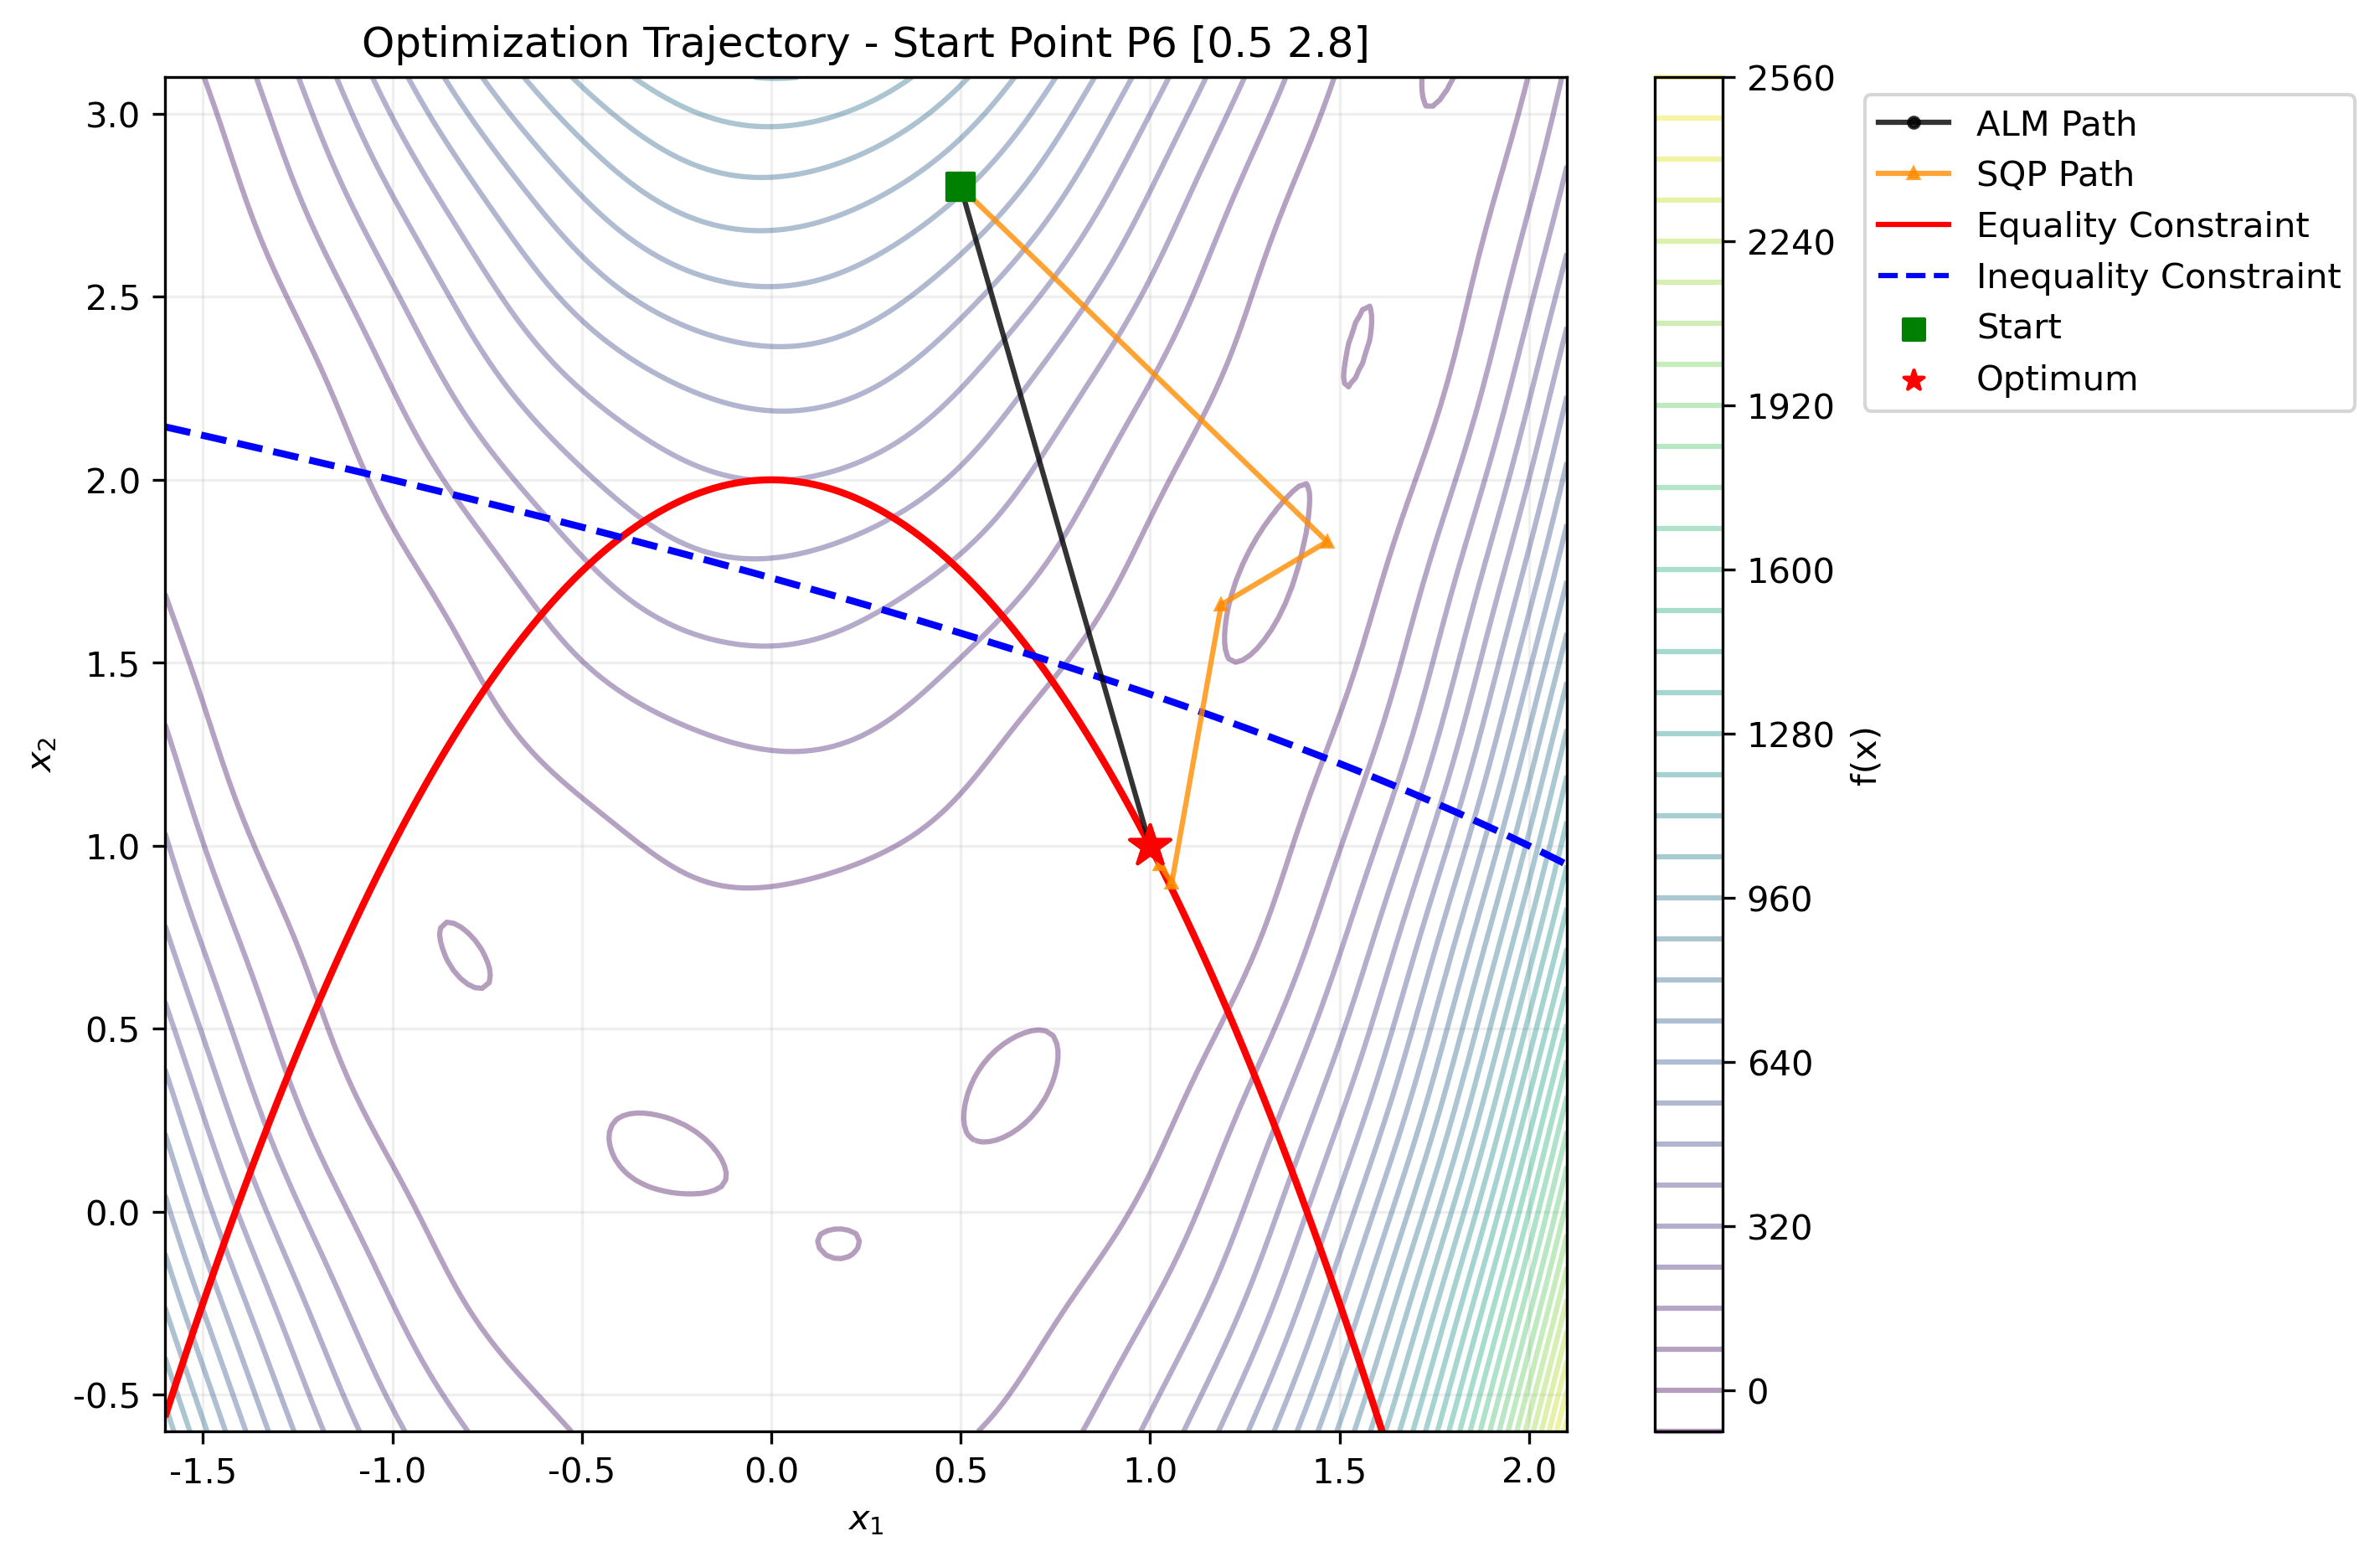
\includegraphics[width=\linewidth]{figures/path_2D_P6.png}
        \caption{P6: Start $[0.5, 2.8]$ (高处收敛)}
        \label{subfig:p6}
    \end{subfigure}
    
    \caption{优化路径可视化分析。图中红色实线为抛物线等式约束，蓝色虚线为线性不等式约束。黑色路径为 ALM，橙色路径为 SQP。}
    \label{fig:traj_analysis}
\end{figure}

% \mbox{} 用于占据一个不可见的位，\\ 强制换行
\paragraph{结果分析：} \mbox{} \\

基于图 \ref{fig:traj_analysis} 的实验结果，针对 ALM 与 SQP 两种算法在非凸约束环境下的收敛行为分析如下：

\begin{enumerate}
    \item \textbf{初值依赖性与局部极小陷阱：}
    图 (a) 与 (d) 显示，当初始点（如 $P_1, P_4$）位于左侧局部极小值的吸引域深处时，受中间非凸势垒的阻隔，ALM 与 SQP 均无法越过函数脊背，最终收敛于局部驻点。这证实了此类基于梯度的局部收敛算法对初值的高度依赖性，在非凸优化中需配合多初值（Multi-start）策略以规避局部陷阱。

    \item \textbf{迭代路径的几何特征差异：}
    观察图 (b)、(e) 及 (f) 中 $P_2, P_5, P_6$ 的轨迹可知，ALM（黑线）呈现“贴壁行走”特征，算法通过惩罚项在目标函数下降与约束违反间取得平衡，沿约束流形表面平滑渐进至最优点，导致收敛速度较慢。相比之下，SQP（橙线）表现为“折线跳跃”，利用牛顿步长在可行域外快速逼近约束流形的切平面，展现出更高效的计算特性。

    \item \textbf{二阶信息的全局探索优势：}
    $P_3$ 点 $[0,0]$ 的演化轨迹（图 c）揭示了两者的核心机制差异。ALM 仅依赖一阶梯度信息，被约束曲面吸附并滑向左侧次优解；而 SQP 通过二次规划子问题利用 Hessian 矩阵近似了全局曲率，准确预判了右侧全局最优解的存在并产生大幅度跨越。该现象强有力地证明了引入二阶信息能显著提升算法在强非线性及鞍点附近的探索能力与鲁棒性。
\end{enumerate}


\subsection{4维 Constrained Rosenbrock函数测试结果}

\subsubsection{实验数据统计}

对于4维测试函数，我们选取了10个不同的初始点进行测试,完整数据请见附录 \ref{app:data}。。该问题包含线性等式约束和线性不等式约束，以及目标函数中的非线性项。
表 \ref{tab:4d_results} 展示了P1-P6测试点在 ALM 和 SQP 算法下的详细运行结果。


\begin{table}[H]
    \centering
    \caption{4D 测试函数优化结果对比}
    \label{tab:4d_results}
    \resizebox{\textwidth}{!}{
    \begin{tabular}{cccccccc}
    \toprule
    \textbf{初始点ID} & \textbf{坐标} & \textbf{算法} & \textbf{迭代次数} & \textbf{最终目标值 $f(x^*)$} & \textbf{总约束违反度} & \textbf{梯度范数 $\|\nabla f\|$} & \textbf{收敛状态} \\
    \midrule
    \multirow{2}{*}{P1} & \multirow{2}{*}{$[0, 0, 0, 0]$} 
      & ALM & 1000 & 0.5281 & $5.81\times 10^{-12}$ & 1.269 & MaxIter \\
      & & SQP & 16 & 0.5281 & 0.0 & 1.269 & Converged (Boundary) \\
    \midrule
    \multirow{2}{*}{P2} & \multirow{2}{*}{$[1, 1, 1, 1]$} 
      & ALM & 1000 & 0.5281 & $3.38\times 10^{-12}$ & 1.269 & MaxIter \\
      & & SQP & 15 & 0.5281 & 0.0 & 1.269 & Converged (Boundary) \\
    \midrule
    \multirow{2}{*}{P3} & \multirow{2}{*}{$[-0.5, 0.5, -0.5, 0.5]$} 
      & ALM & 1000 & 0.5281 & $1.08\times 10^{-12}$ & 1.269 & MaxIter \\
      & & SQP & 16 & 0.5281 & 0.0 & 1.269 & Converged (Boundary) \\
    \midrule
    \multirow{2}{*}{P4} & \multirow{2}{*}{$[0.5, 0.5, 0.5, 0.5]$} 
      & ALM & 1000 & 0.5281 & $3.38\times 10^{-12}$ & 1.269 & MaxIter \\
      & & SQP & 13 & 0.5281 & 0.0 & 1.269 & Converged (Boundary) \\
    \midrule
    \multirow{2}{*}{P5} & \multirow{2}{*}{$[1.2, -0.2, 1.2, -0.2]$} 
      & ALM & 1000 & 0.5281 & $5.91\times 10^{-12}$ & 1.269 & MaxIter \\
      & & SQP & 17 & 0.5281 & $2.22\times 10^{-16}$ & 1.269 & Converged (Boundary) \\
    \midrule
    \multirow{2}{*}{P6} & \multirow{2}{*}{$[-1, -1, -1, -1]$} 
      & ALM & 1000 & 0.5281 & $2.97\times 10^{-12}$ & 1.269 & MaxIter \\
      & & SQP & 22 & 0.5281 & $2.22\times 10^{-16}$ & 1.269 & Converged (Boundary) \\
    \bottomrule
    \end{tabular}
    }
    {\footnotesize
\begin{flushleft} % 强制左对齐
    \textbf{表格注释说明：}在实验数据统计表中，状态标识定义如下：
    \begin{itemize}
        \setlength\itemsep{0pt}  % 让列表更紧凑
        \setlength\parsep{0pt}   % 去除段落间距
        \setlength{\leftmargin}{1.5em} % 控制左侧缩进，如果觉得缩进太多可调小
        \item \textbf{Success}：算法在最大迭代次数内成功满足 KKT 条件及约束精度要求，收敛至最优点。
        \item \textbf{Converged (Boundary)}：算法收敛于可行域边界上的某一点（通常对应不等式约束激活的情况）。
        \item \textbf{MaxIter}：算法达到预设的最大迭代次数停止。
    \end{itemize}
    \textbf{注：}ALM 虽达到最大迭代次数，但约束违反度均已满足精度要求，主要为梯度条件未满足。
\end{flushleft}
}
\end{table}



\paragraph{结果分析}

\begin{enumerate}
    \item \textbf{收敛点的一致性与单峰特性}：
    与 2D 函数出现局部最优不同，在 4D 测试中，无论初始点选取何值，两种算法最终均收敛至同一个坐标点 $x^* \approx [0.7973, 0.6364, 0.4052, 0.1610]$，对应的目标函数值均为 $0.528086$。这表明在该约束条件限定的可行域内，该测试函数很可能只存在唯一的全局极小值，或者该极小值的吸引域非常大。

    \item \textbf{约束边界上的最优解}：
    所有收敛点的目标函数梯度 $\nabla f(x^*)$ 均不为 0。结合 SQP 的收敛状态，可以确认最优解位于约束边界上。

    \item \textbf{算法性能差异}：
    \begin{itemize}
        \item \textbf{SQP (序列二次规划)}：表现出极高的效率，迭代次数仅在 13 到 22 次之间。由于该 4D 问题的约束包含线性等式和线性不等式，SQP 的二次规划子问题（QP）能够精确处理这些线性约束，使得搜索方向始终贴合或指向可行域边界，从而实现了快速收敛。其最终约束违反度几乎为 0（$10^{-16}$ 级别），显示了数值上的精确性。
        \item \textbf{ALM (增广拉格朗日法)}：在所有 6 个测试点中均运行至 $k_{max}=1000$。尽管如此，ALM 最终求得的目标函数值与 SQP 几乎一致，且约束违反度控制在 $10^{-12}$ 量级，说明算法实际上已经找到了最优解。未能提前终止的原因可能是因为最优解位于边界上，导致拉格朗日乘子的更新需要较多次迭代才能使得拉格朗日函数的梯度范数 $\|\nabla L\|$ 严格小于 $10^{-6}$，或者是外层罚参数 $\sigma$ 的更新策略在处理此类边界解时收敛较慢。
    \end{itemize}
\end{enumerate}

\subsubsection{算法收敛曲线对比}
图 \ref{fig:4d_convergence} 展示了算法从 6 个不同初始点 ($P1 \sim P6$) 出发的收敛过程。

% --- 第一部分：包含 P1 和 P2 (全宽显示) ---
\begin{figure}[H]
    \centering
    % P1
    \begin{subfigure}[b]{1.0\textwidth}
        \centering
        % 将宽度设为 1.0\textwidth (即 100% 页面宽度)
        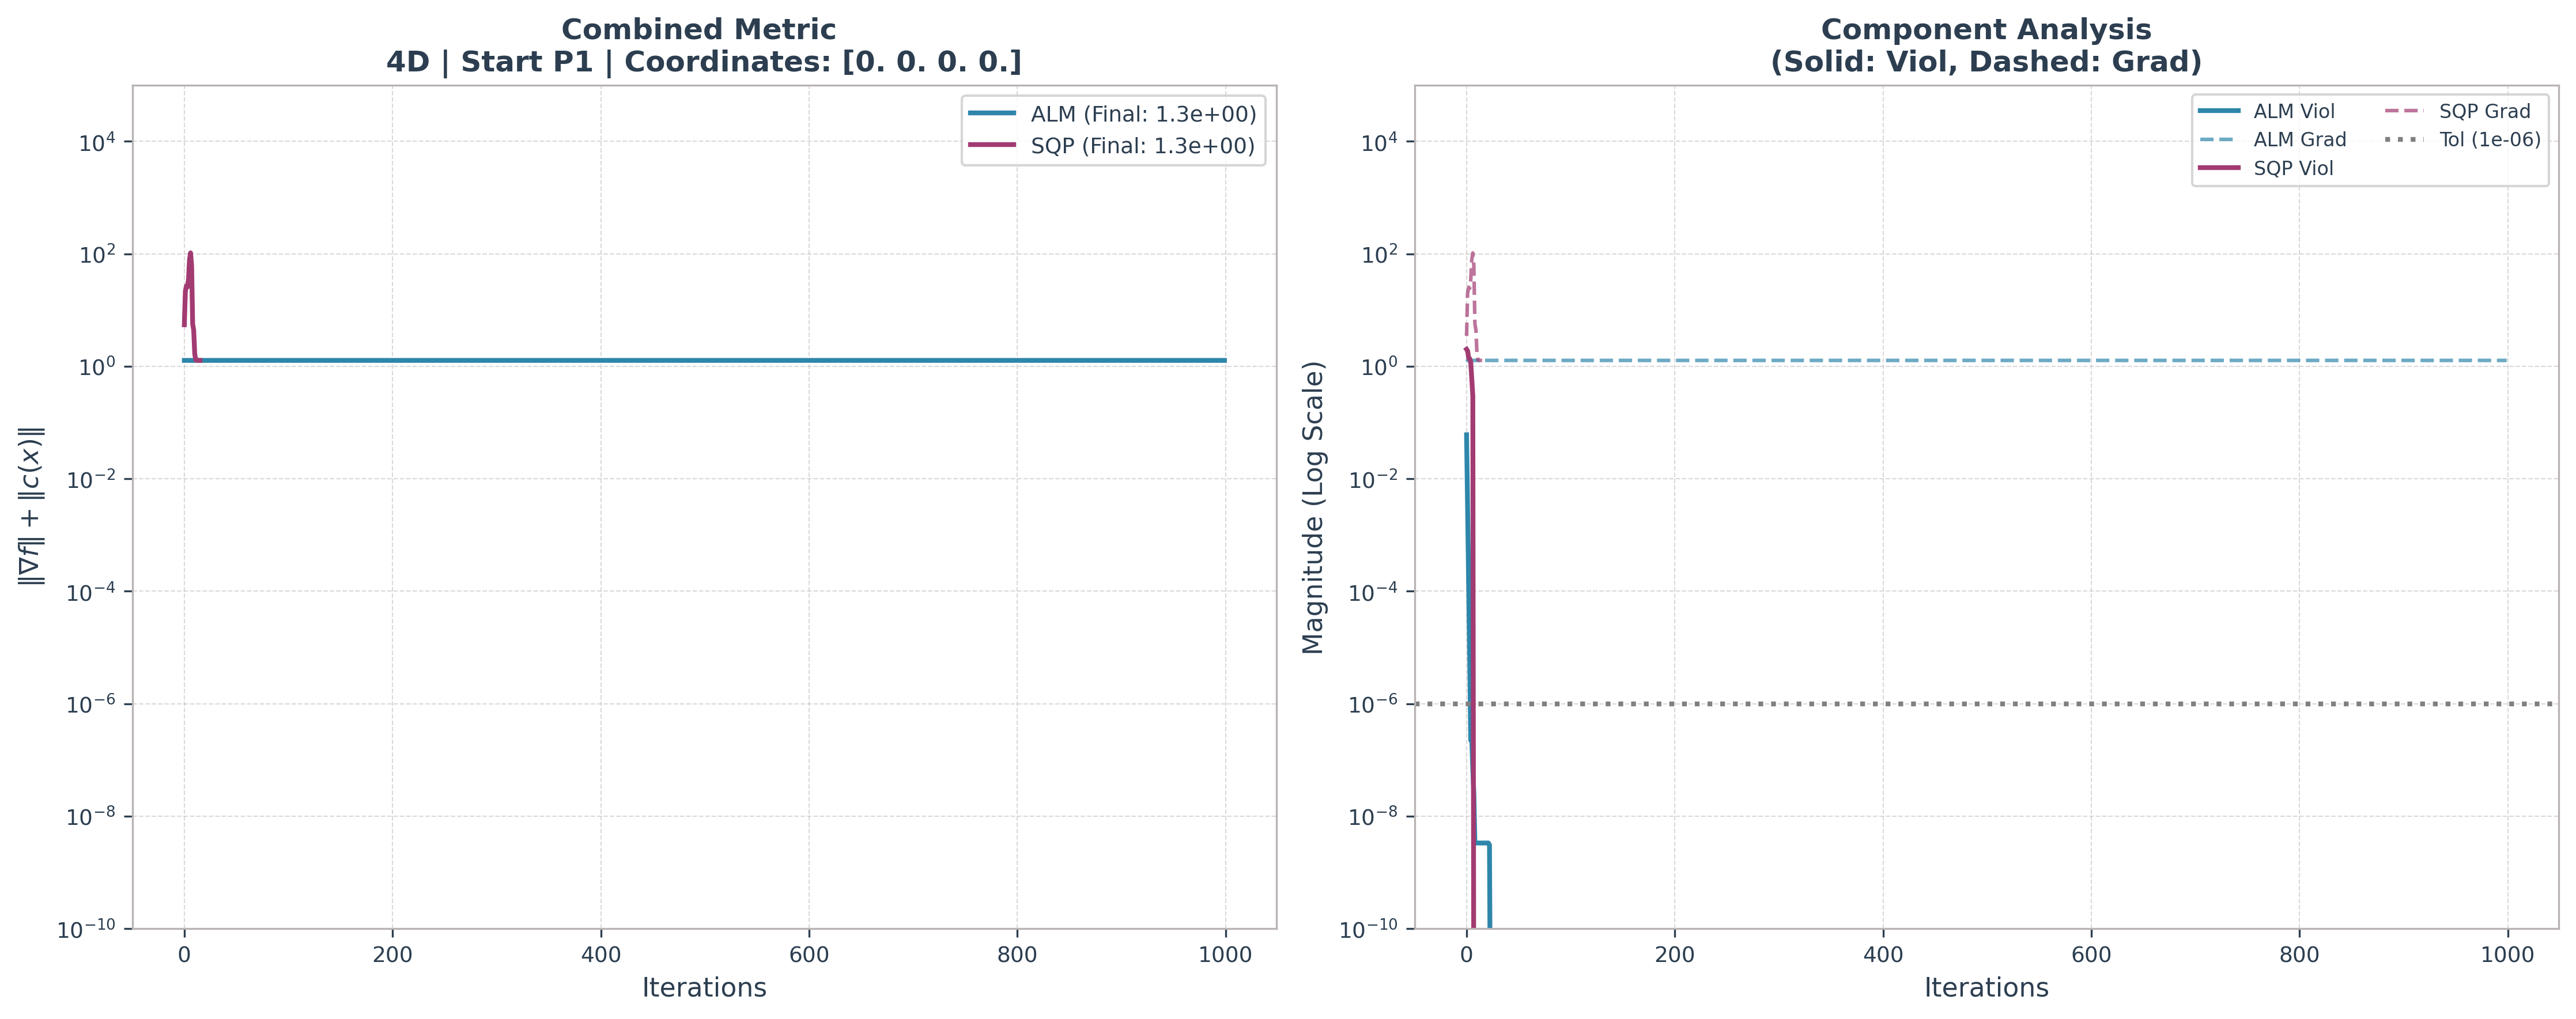
\includegraphics[width=1.0\textwidth]{figures/conv_dual_4D_P1.png}
        \caption{P1: Start $[0, 0, 0, 0]$}
    \end{subfigure}
    
    \vspace{1em} % 图片间距
    
    % P2
    \begin{subfigure}[b]{1.0\textwidth}
        \centering
        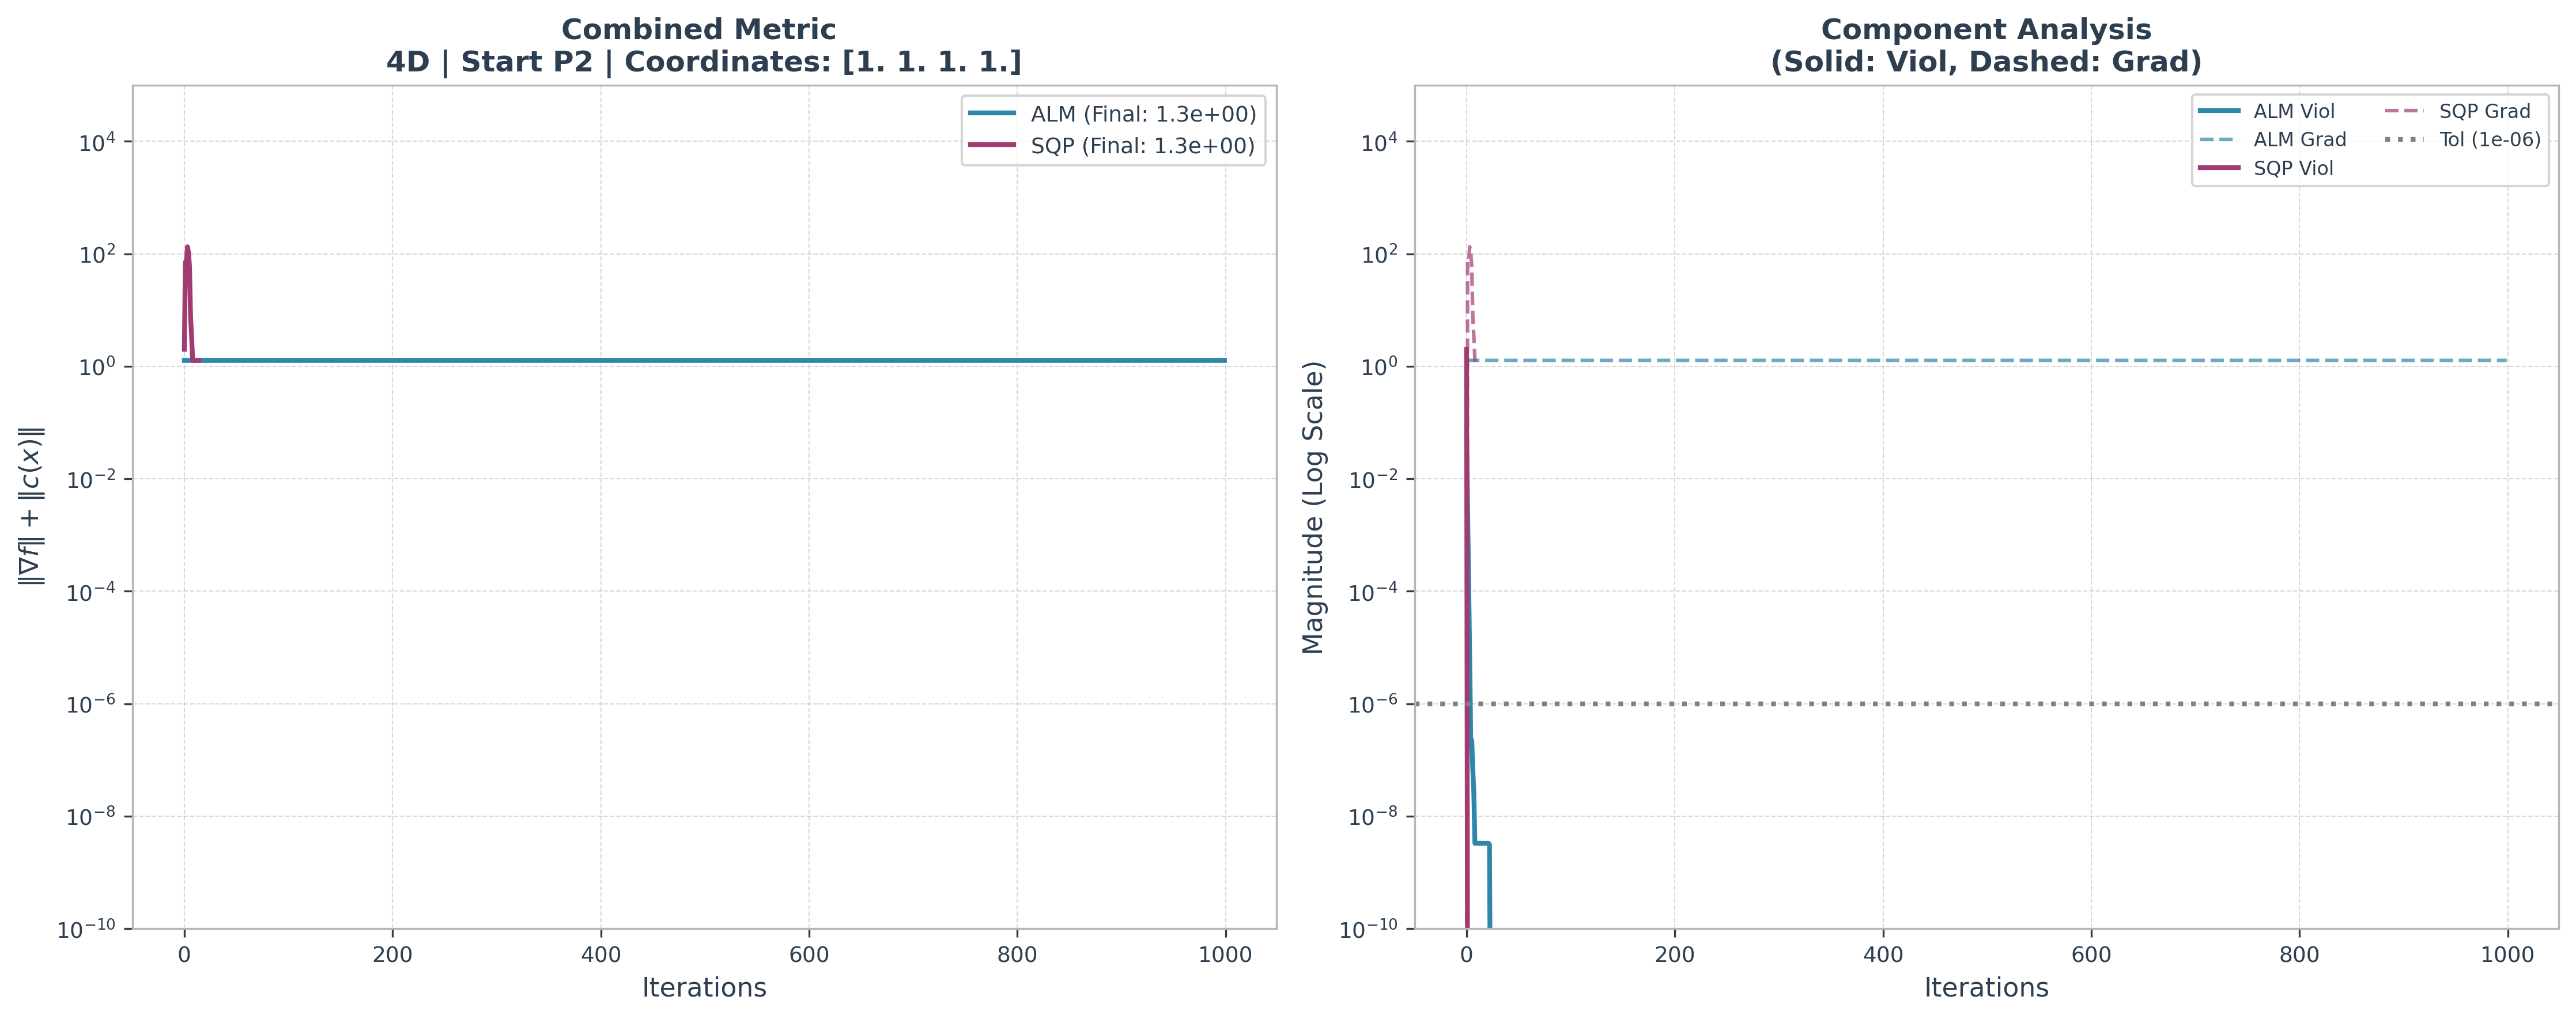
\includegraphics[width=1.0\textwidth]{figures/conv_dual_4D_P2.png}
        \caption{P2: Start $[1, 1, 1, 1]$}
    \end{subfigure}
    
    \caption{ALM与SQP算法在不同初始点下的收敛曲线对比（P1-P2）。}
    \label{fig:4d_convergence}
\end{figure}

% --- 第二部分：包含 P3 和 P4 ---
\begin{figure}[H]
    \ContinuedFloat % 保持编号连续
    \centering
    % \addtocounter{subfigure}{2} # 无需增加计数器
    % P3
    \begin{subfigure}[b]{1.0\textwidth}
        \centering
        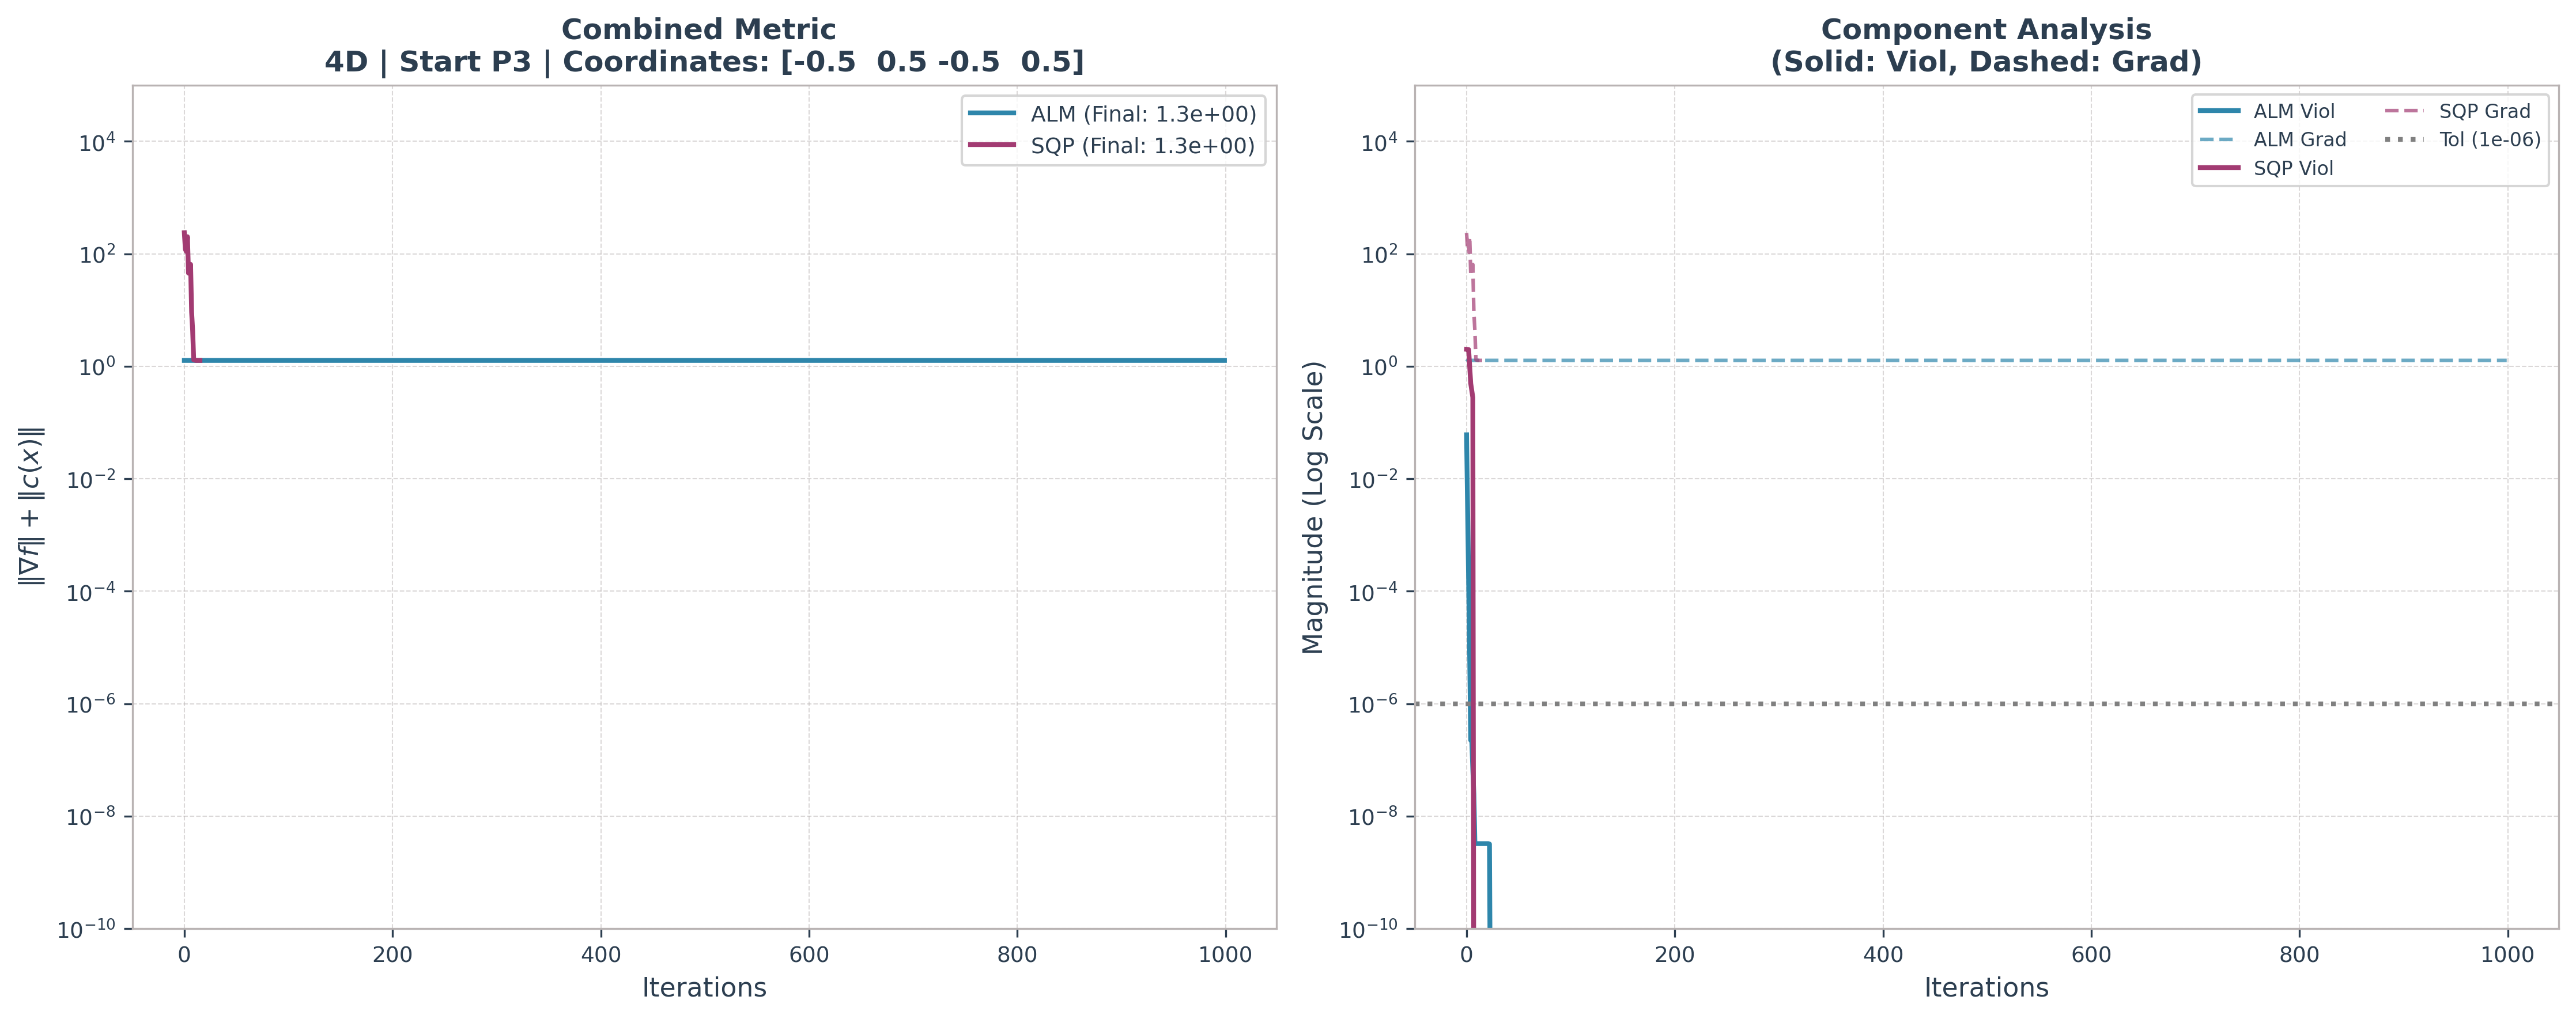
\includegraphics[width=1.0\textwidth]{figures/conv_dual_4D_P3.png}
        \caption{P3: Start $[-0.5, 0.5, -0.5, 0.5]$}
    \end{subfigure}
    
    \vspace{1em}
    
    % P4
    \begin{subfigure}[b]{1.0\textwidth}
        \centering
        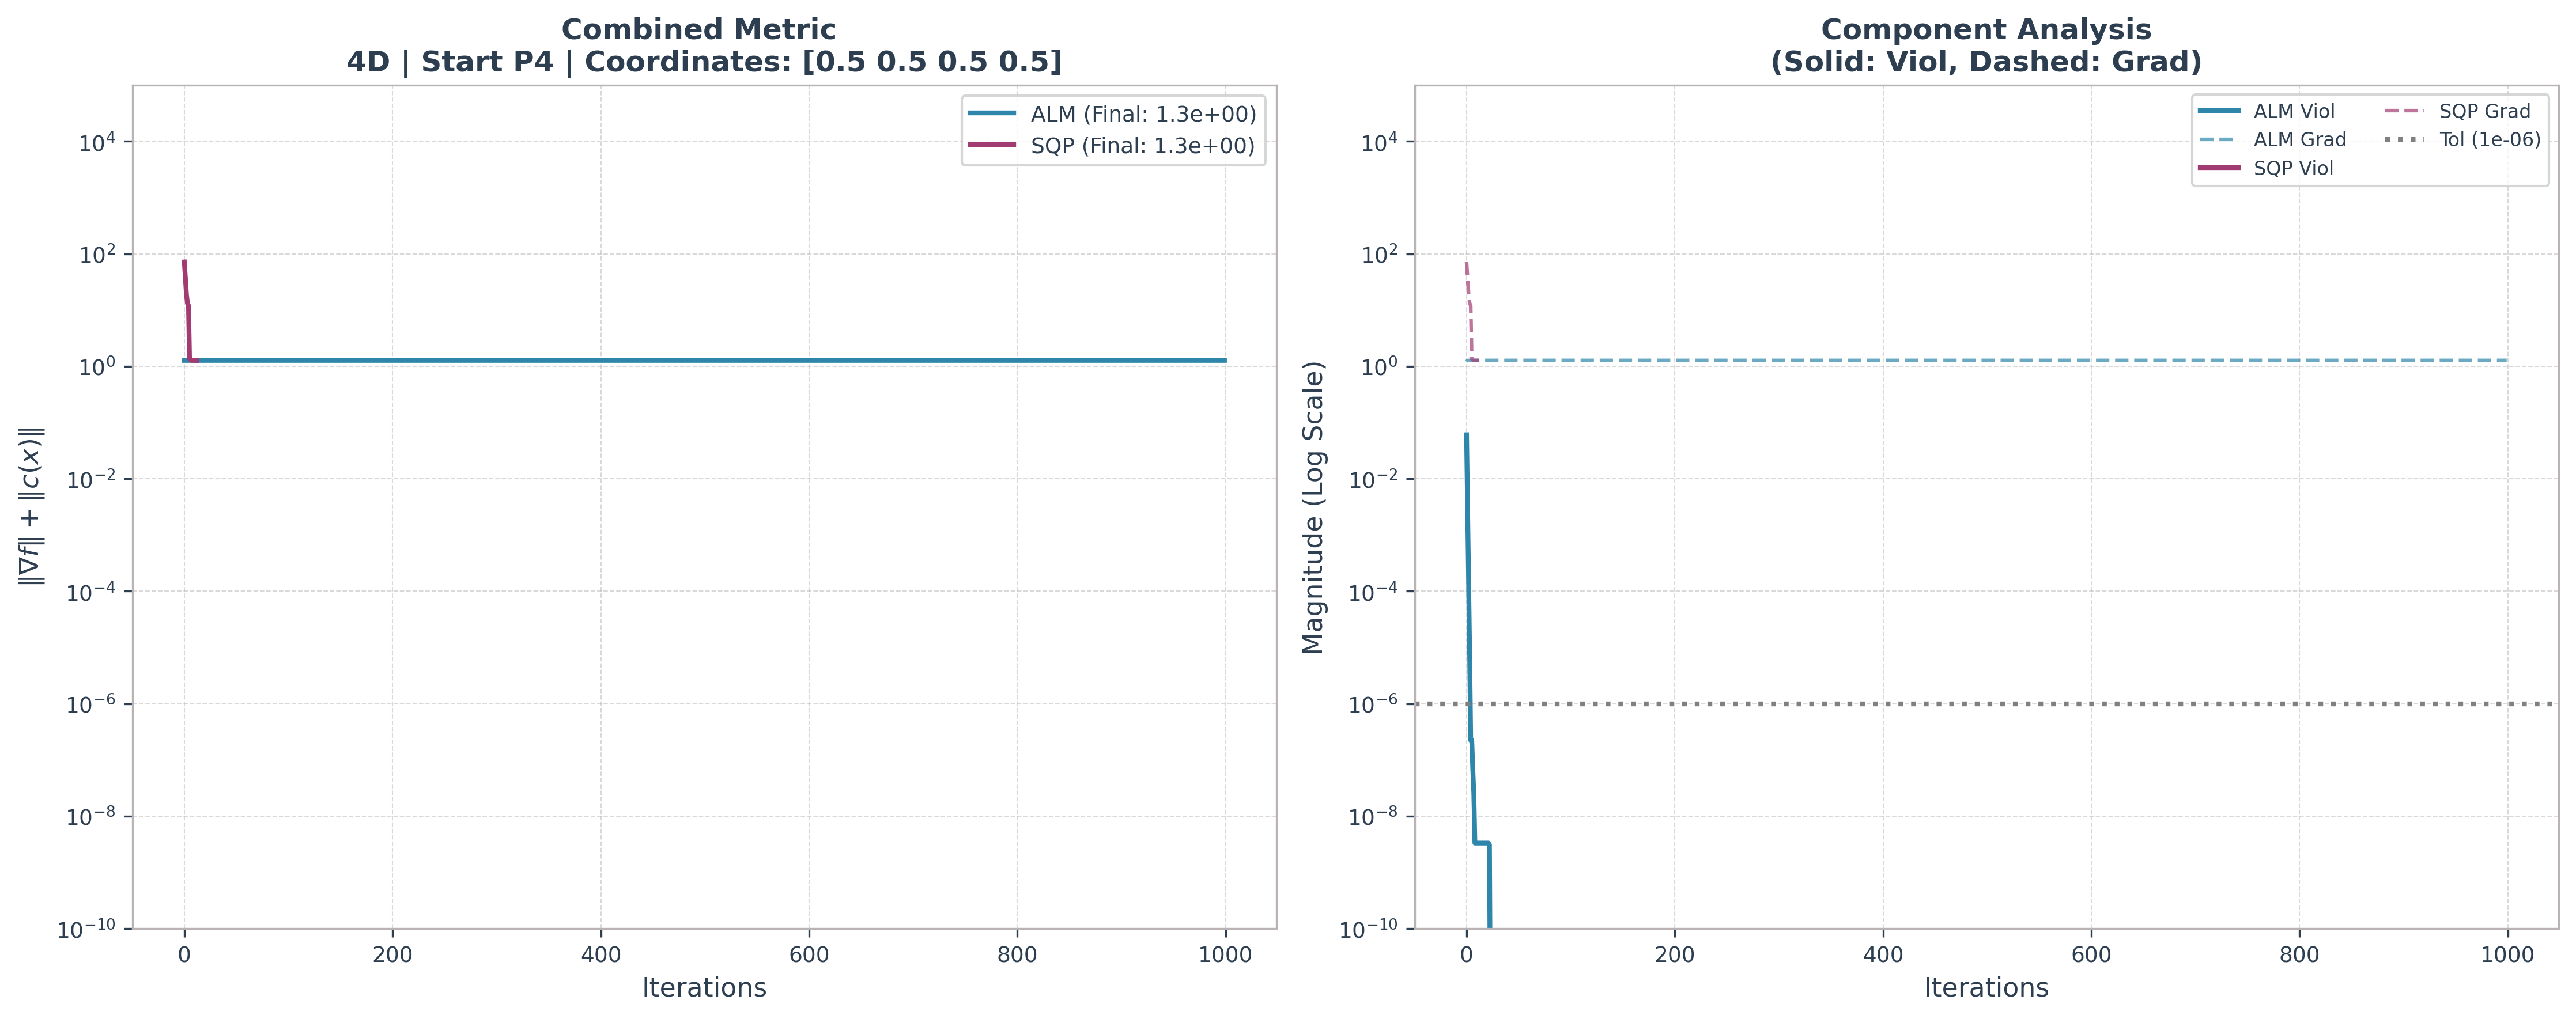
\includegraphics[width=1.0\textwidth]{figures/conv_dual_4D_P4.png}
        \caption{P4: Start $[0.5, 0.5, 0.5, 0.5]$}
    \end{subfigure}
    
    \caption[]{ALM与SQP算法在不同初始点下的收敛曲线对比（续）。}
    % \label{fig:4d_convergence_part2}
\end{figure}

% --- 第三部分：包含 P5 和 P6 ---
\begin{figure}[H]
    \ContinuedFloat % 保持编号连续
    \centering
    % \addtocounter{subfigure}{2} # 无需增加计数器
    % P5
    \begin{subfigure}[b]{1.0\textwidth}
        \centering
        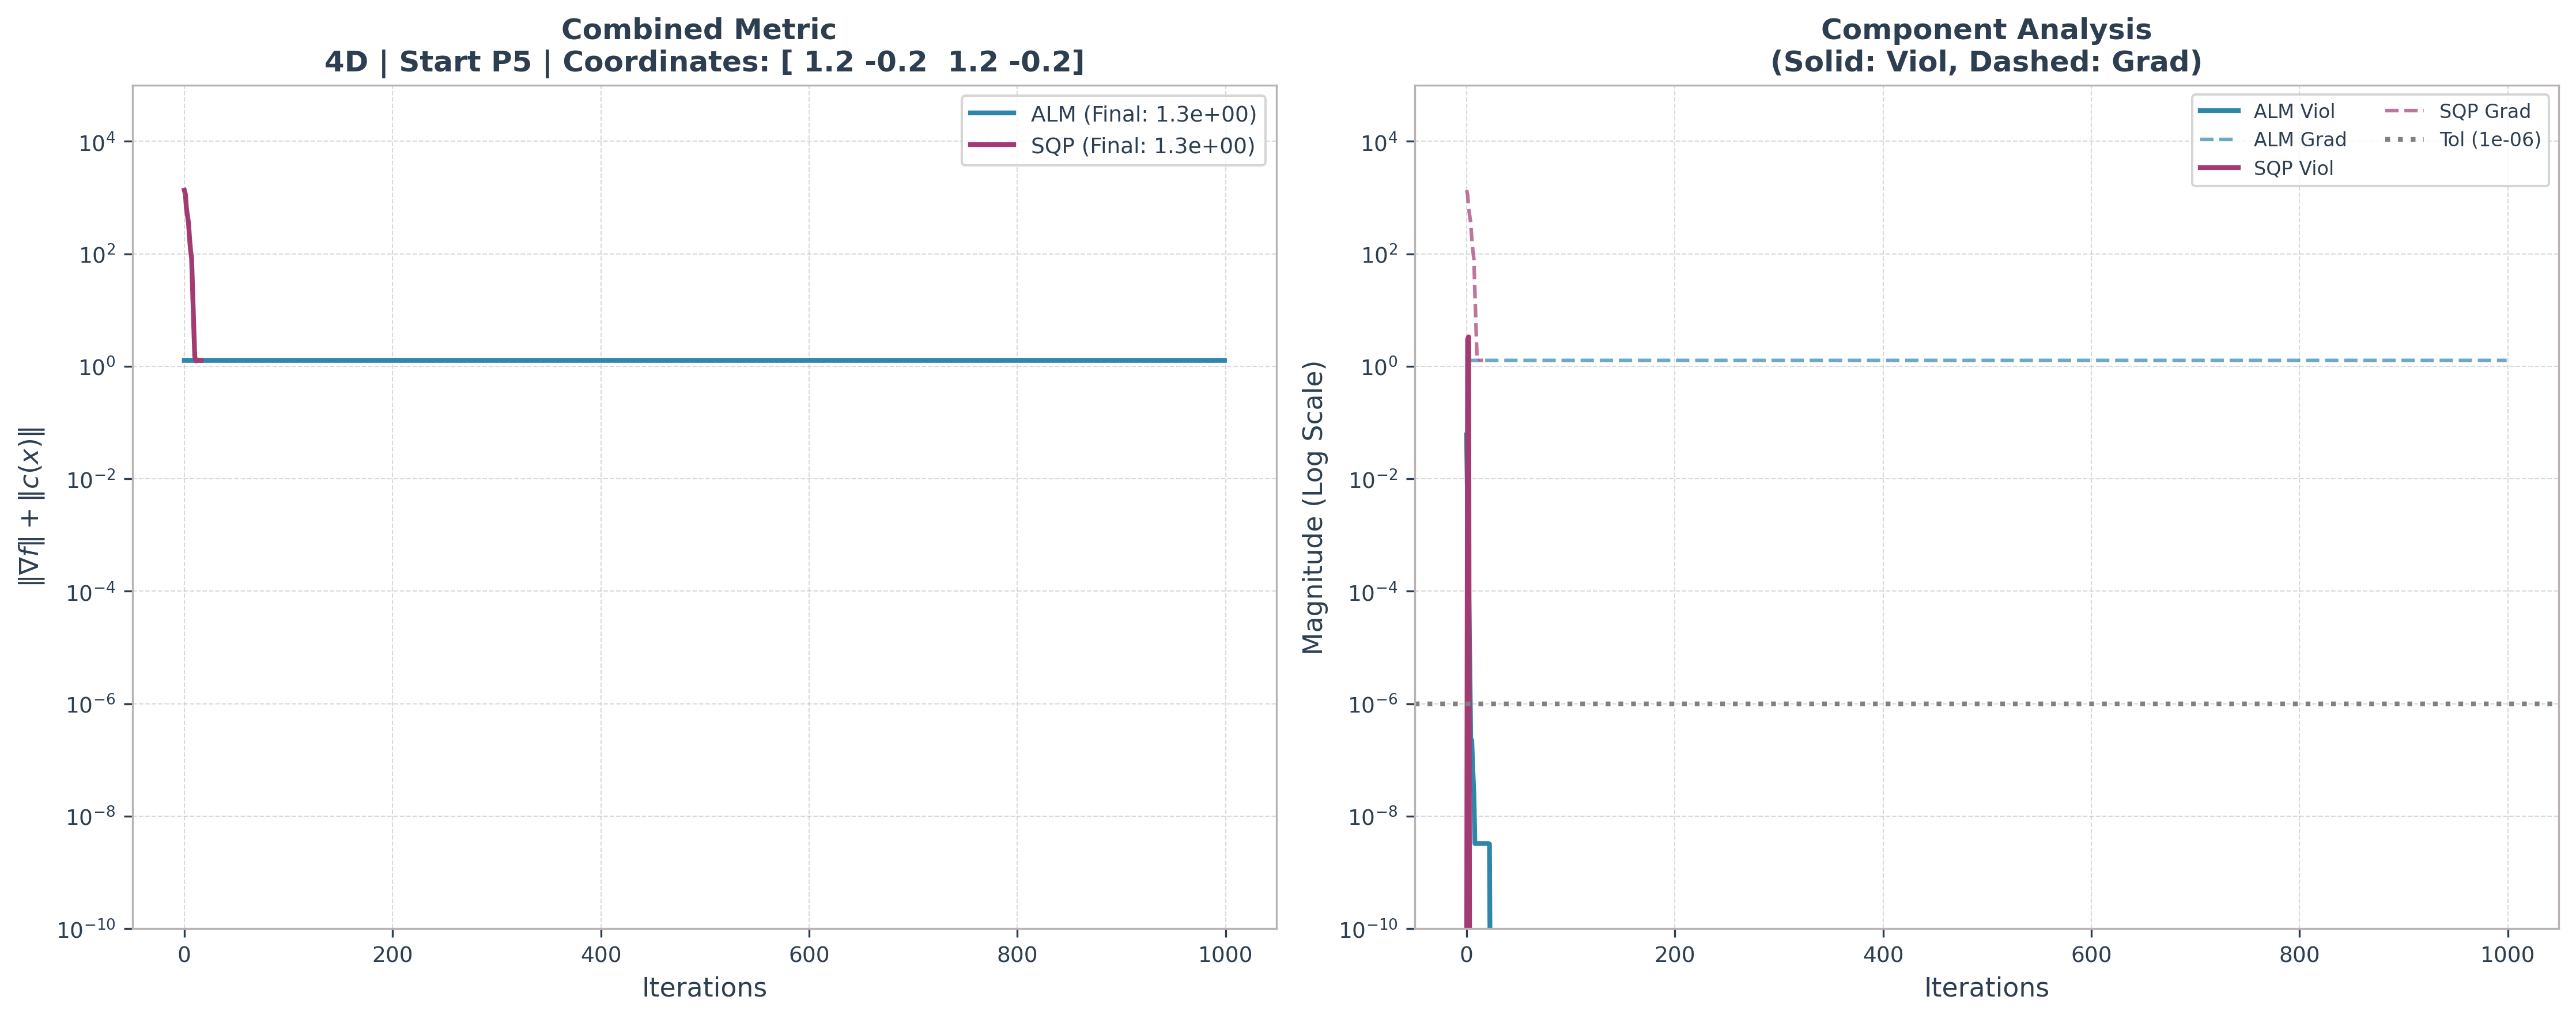
\includegraphics[width=1.0\textwidth]{figures/conv_dual_4D_P5.png}
        \caption{P5: Start $[1.2, -0.2, 1.2, -0.2]$}
    \end{subfigure}
    
    \vspace{1em}
    
    % P6
    \begin{subfigure}[b]{1.0\textwidth}
        \centering
        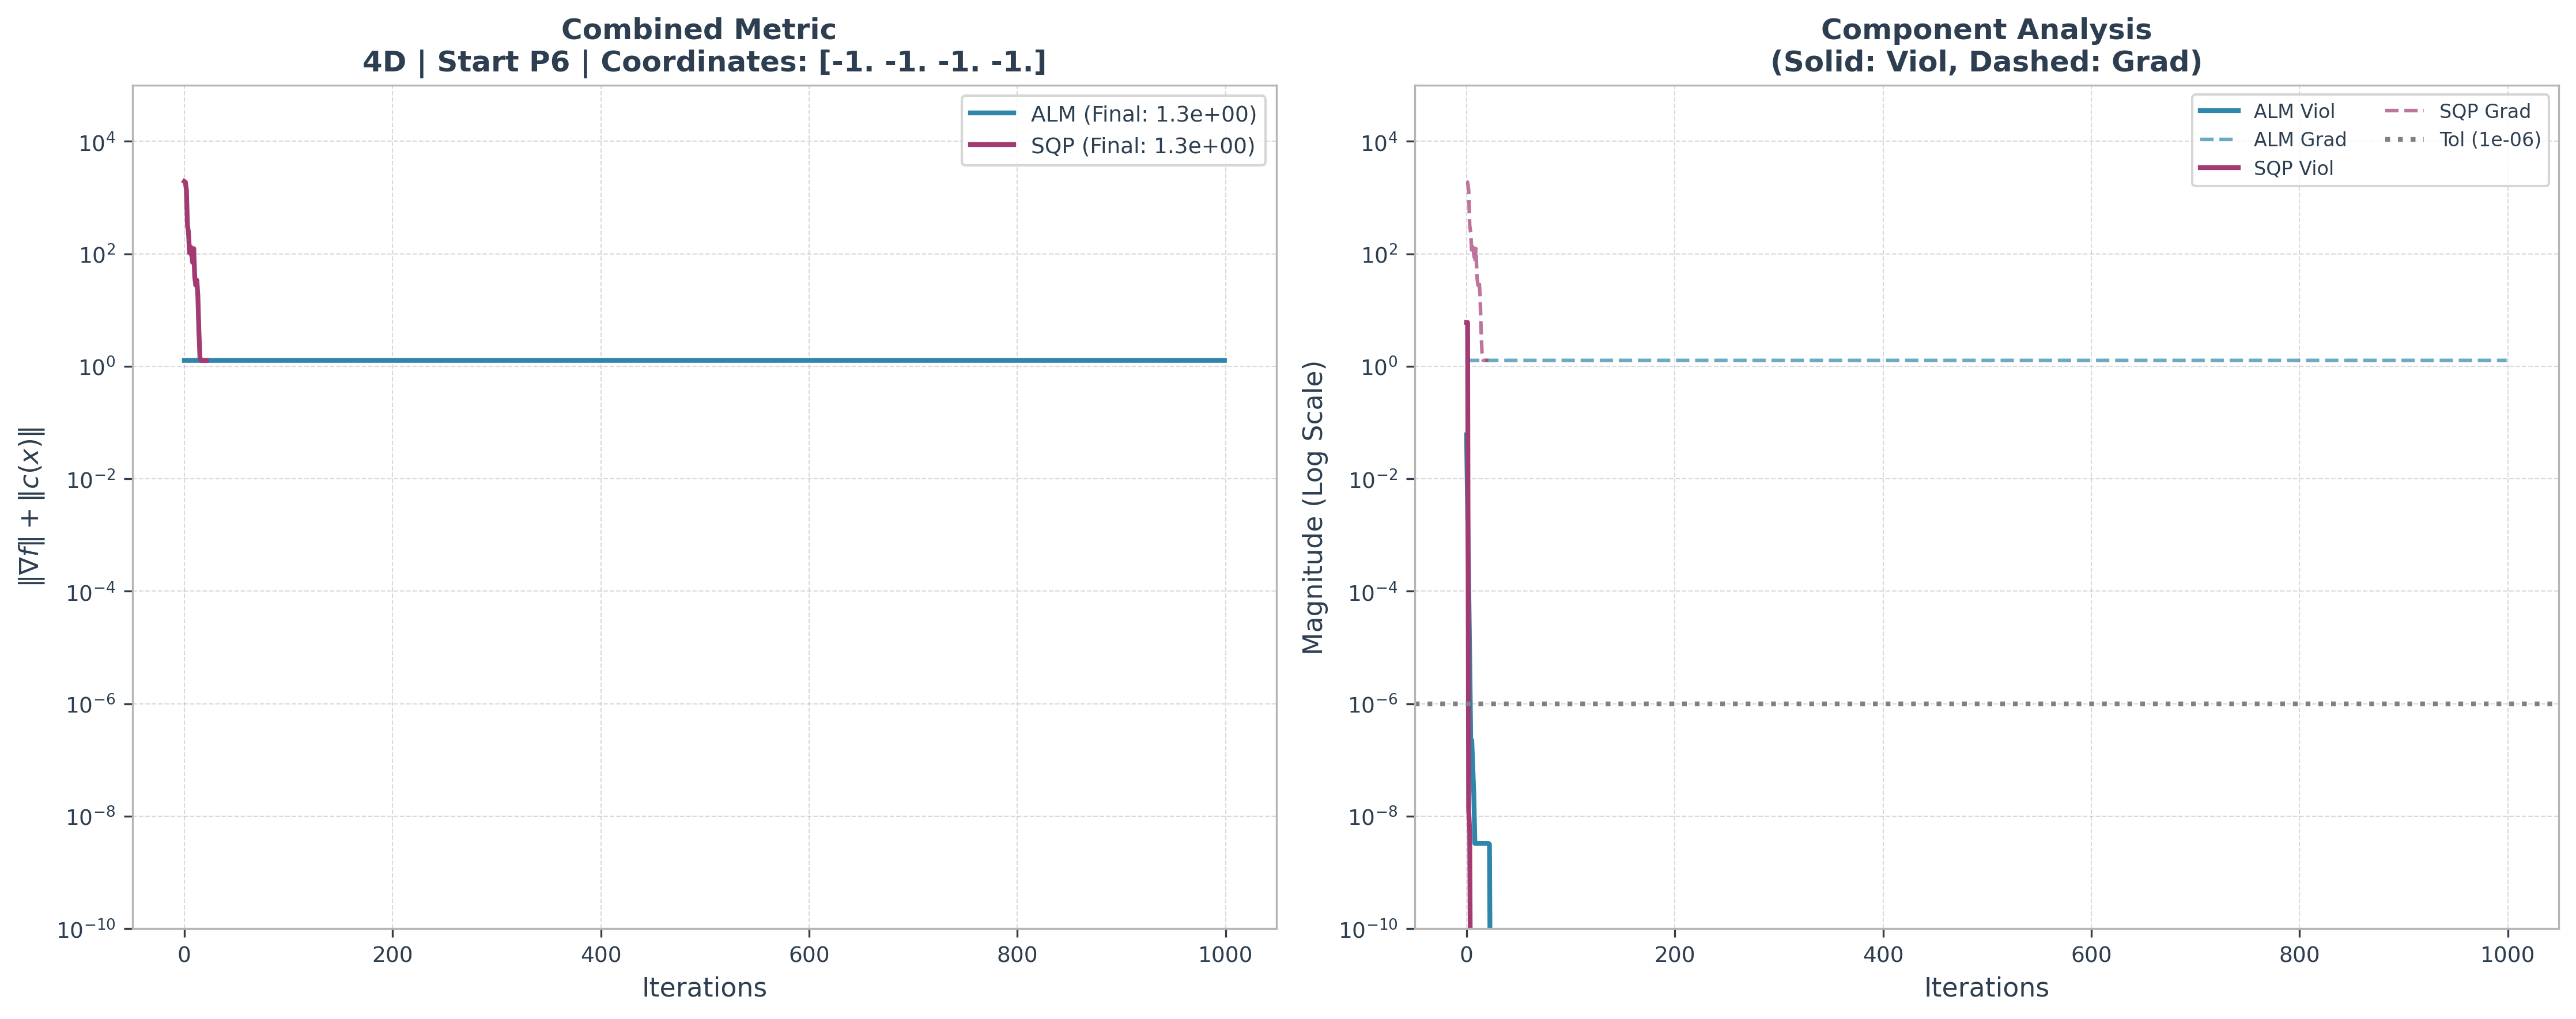
\includegraphics[width=1.0\textwidth]{figures/conv_dual_4D_P6.png}
        \caption{P6: Start $[-1, -1, -1, -1]$}
    \end{subfigure}
    
    \caption[]{ALM与SQP算法在不同初始点下的收敛曲线对比（续）。}
    \label{fig:4d_convergence_part3}
\end{figure}


% \subsubsection{收敛曲线可视化}
% 图 \ref{fig:4d_convergence} 展示了算法从 6 个不同初始点 ($P1 \sim P6$) 出发的收敛过程。

% % --- 第一部分：包含 P1 到 P4 ---
% \begin{figure}[H]
%     \centering
%     % P1
%     \begin{subfigure}[b]{0.48\textwidth}
%         \centering
%         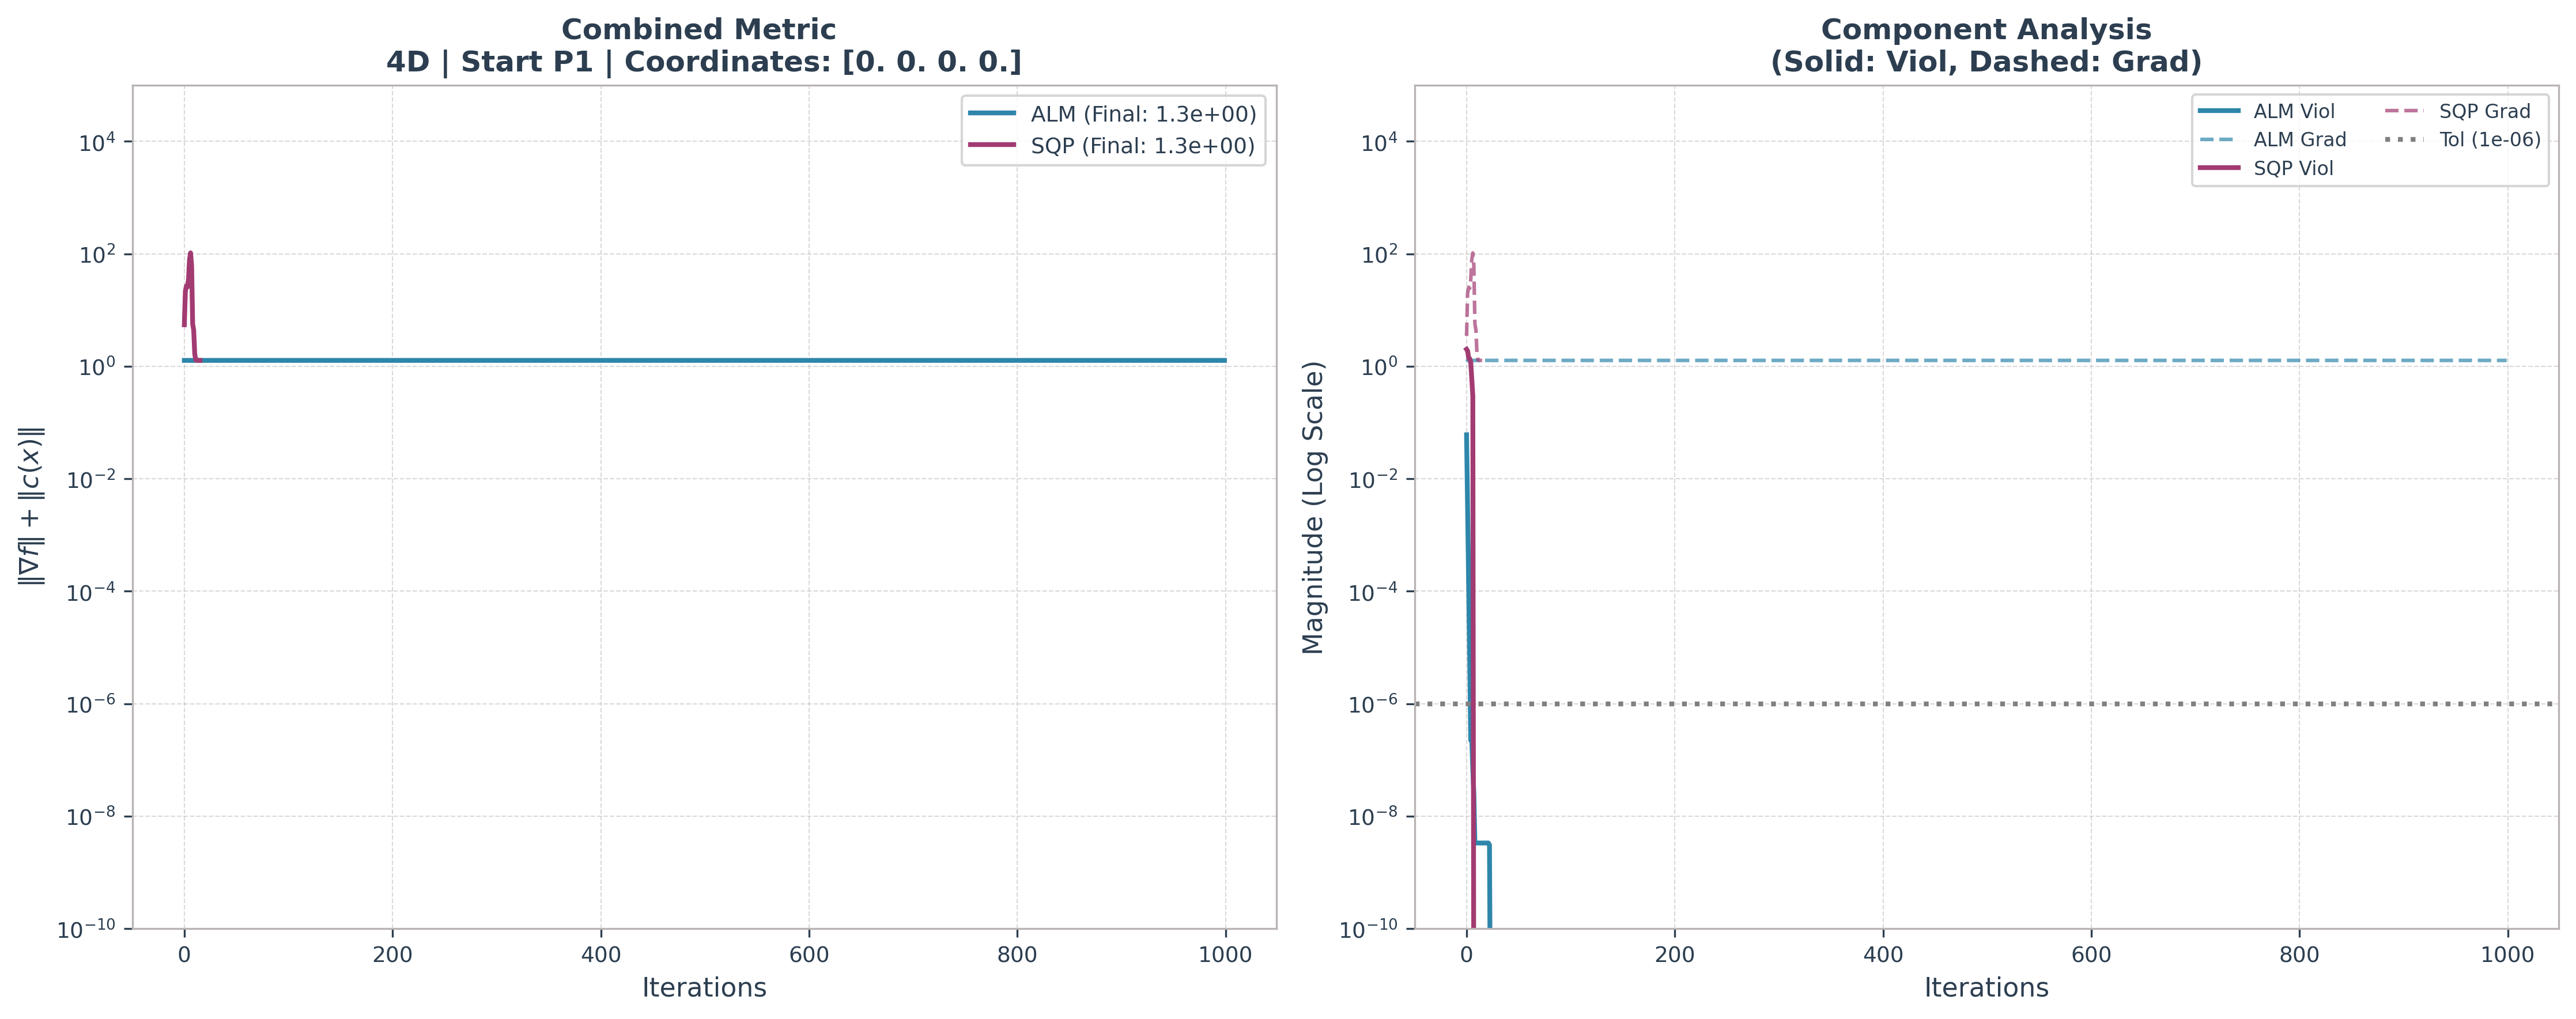
\includegraphics[width=\textwidth]{figures/conv_dual_4D_P1.png}
%         \caption{P1: Start $[0, 0, 0, 0]$}
%     \end{subfigure}
%     \hfill
%     % P2
%     \begin{subfigure}[b]{0.48\textwidth}
%         \centering
%         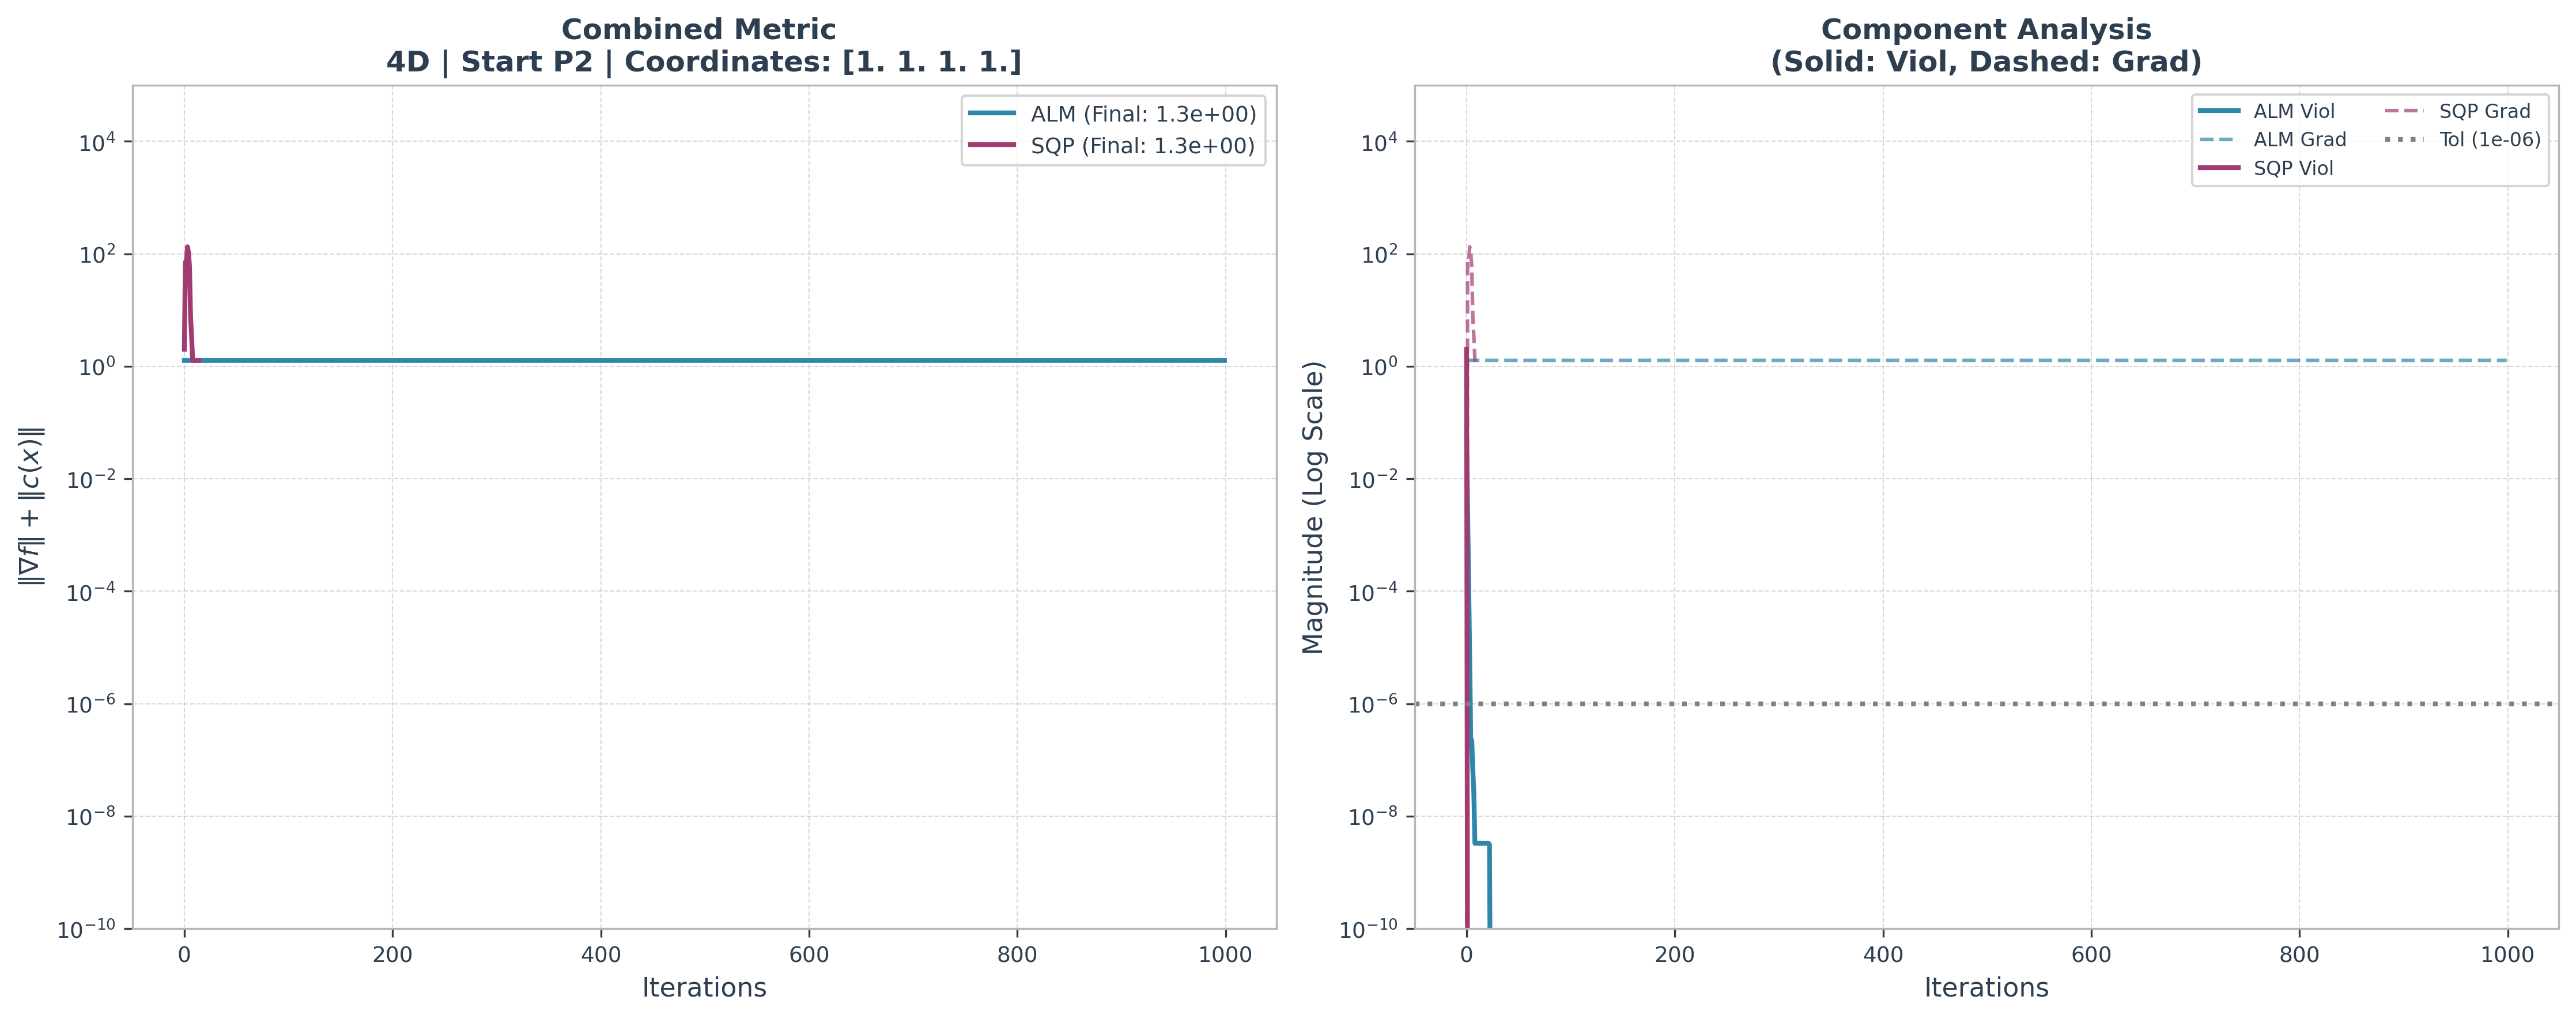
\includegraphics[width=\textwidth]{figures/conv_dual_4D_P2.png}
%         \caption{P2: Start $[1, 1, 1, 1]$}
%     \end{subfigure}
    
%     \vspace{1em} % 增加行间距
    
%     % P3
%     \begin{subfigure}[b]{0.48\textwidth}
%         \centering
%         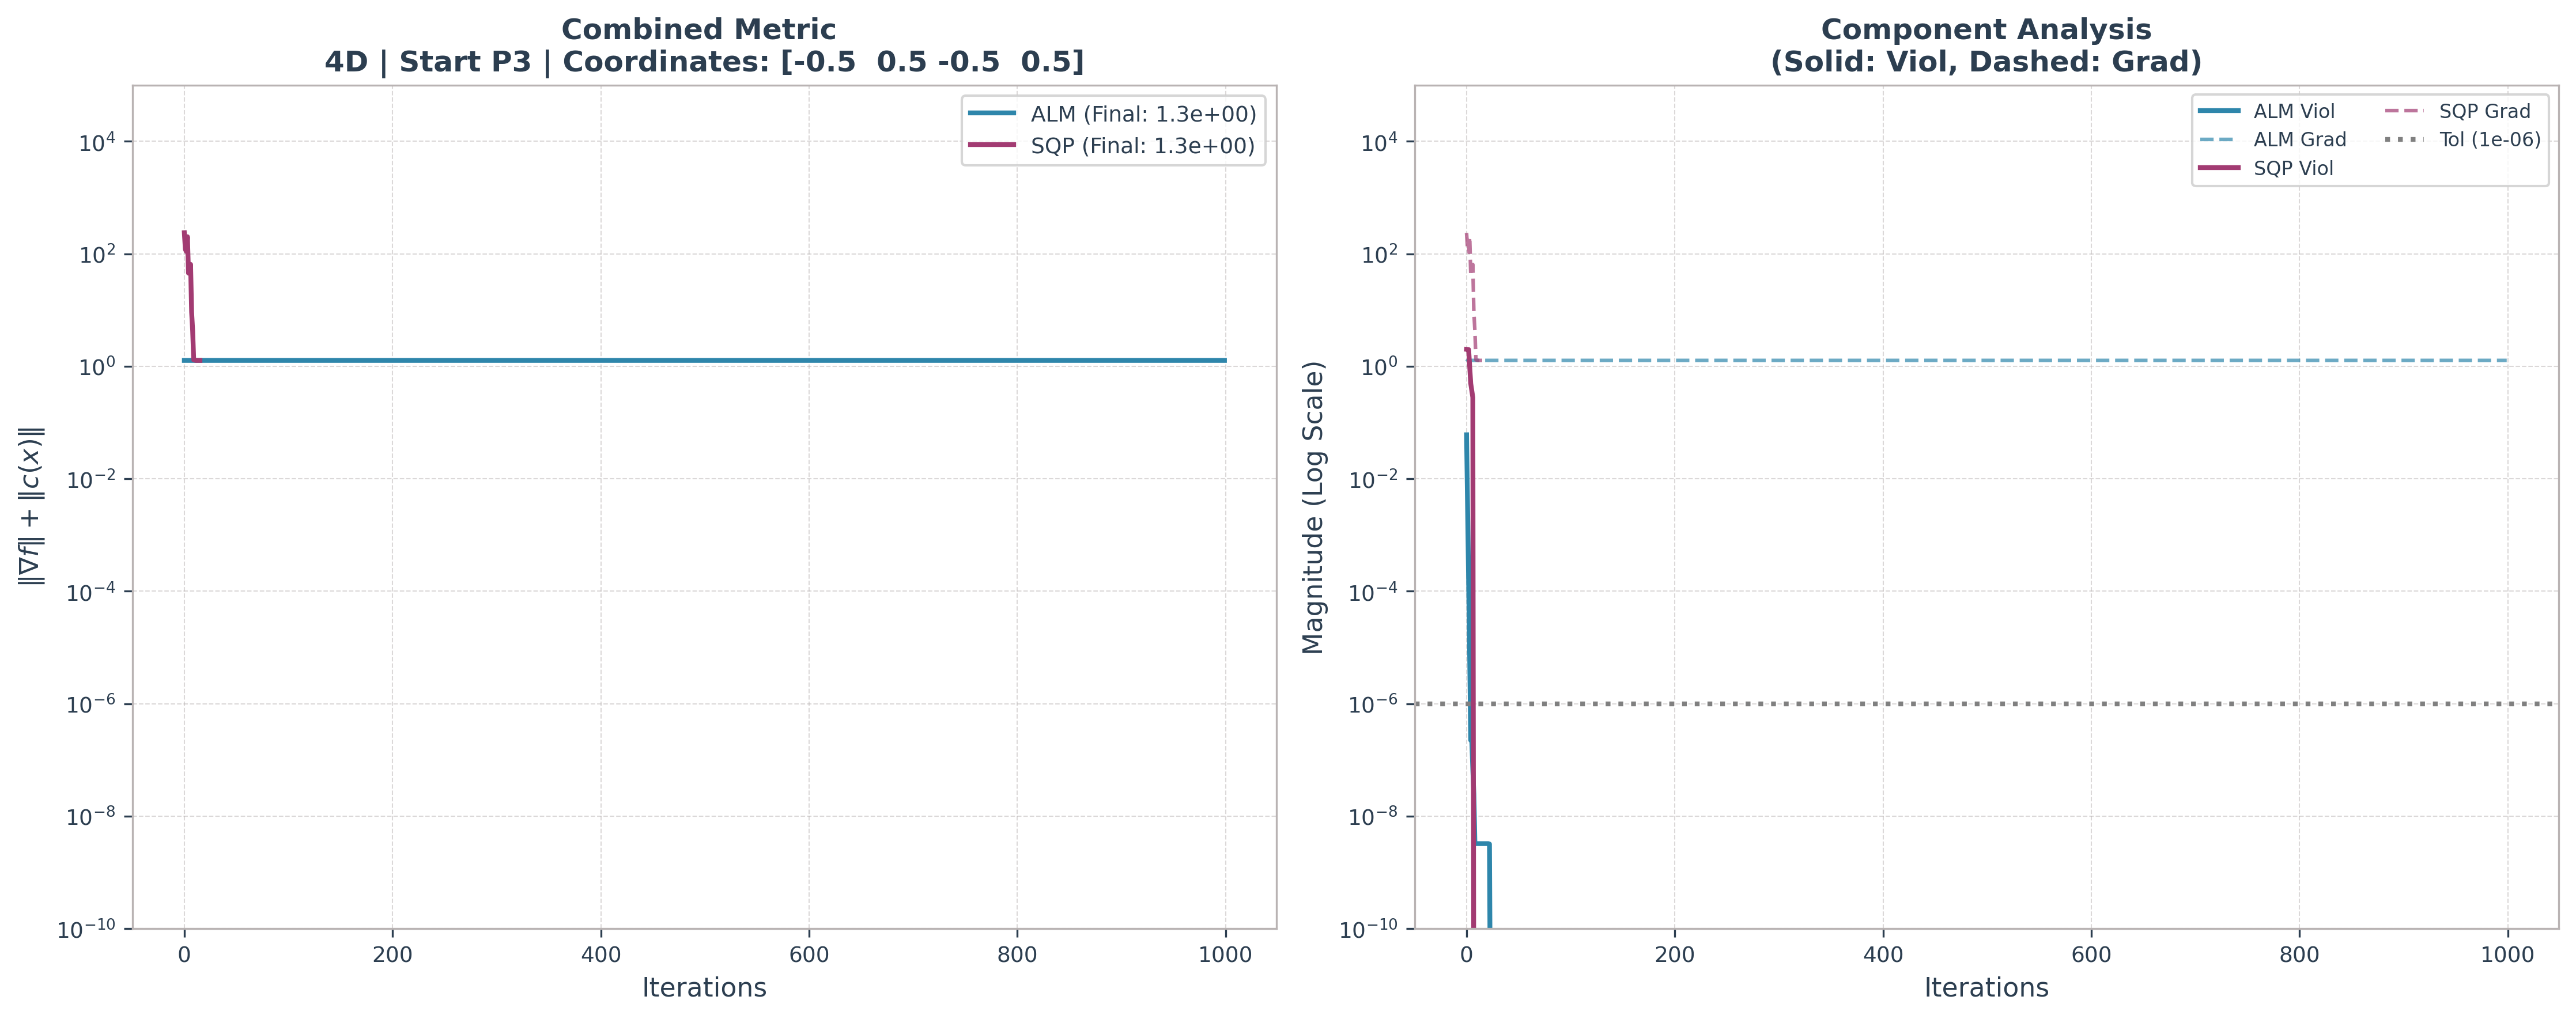
\includegraphics[width=\textwidth]{figures/conv_dual_4D_P3.png}
%         \caption{P3: Start $[-0.5, 0.5, -0.5, 0.5]$}
%     \end{subfigure}
%     \hfill
%     % P4
%     \begin{subfigure}[b]{0.48\textwidth}
%         \centering
%         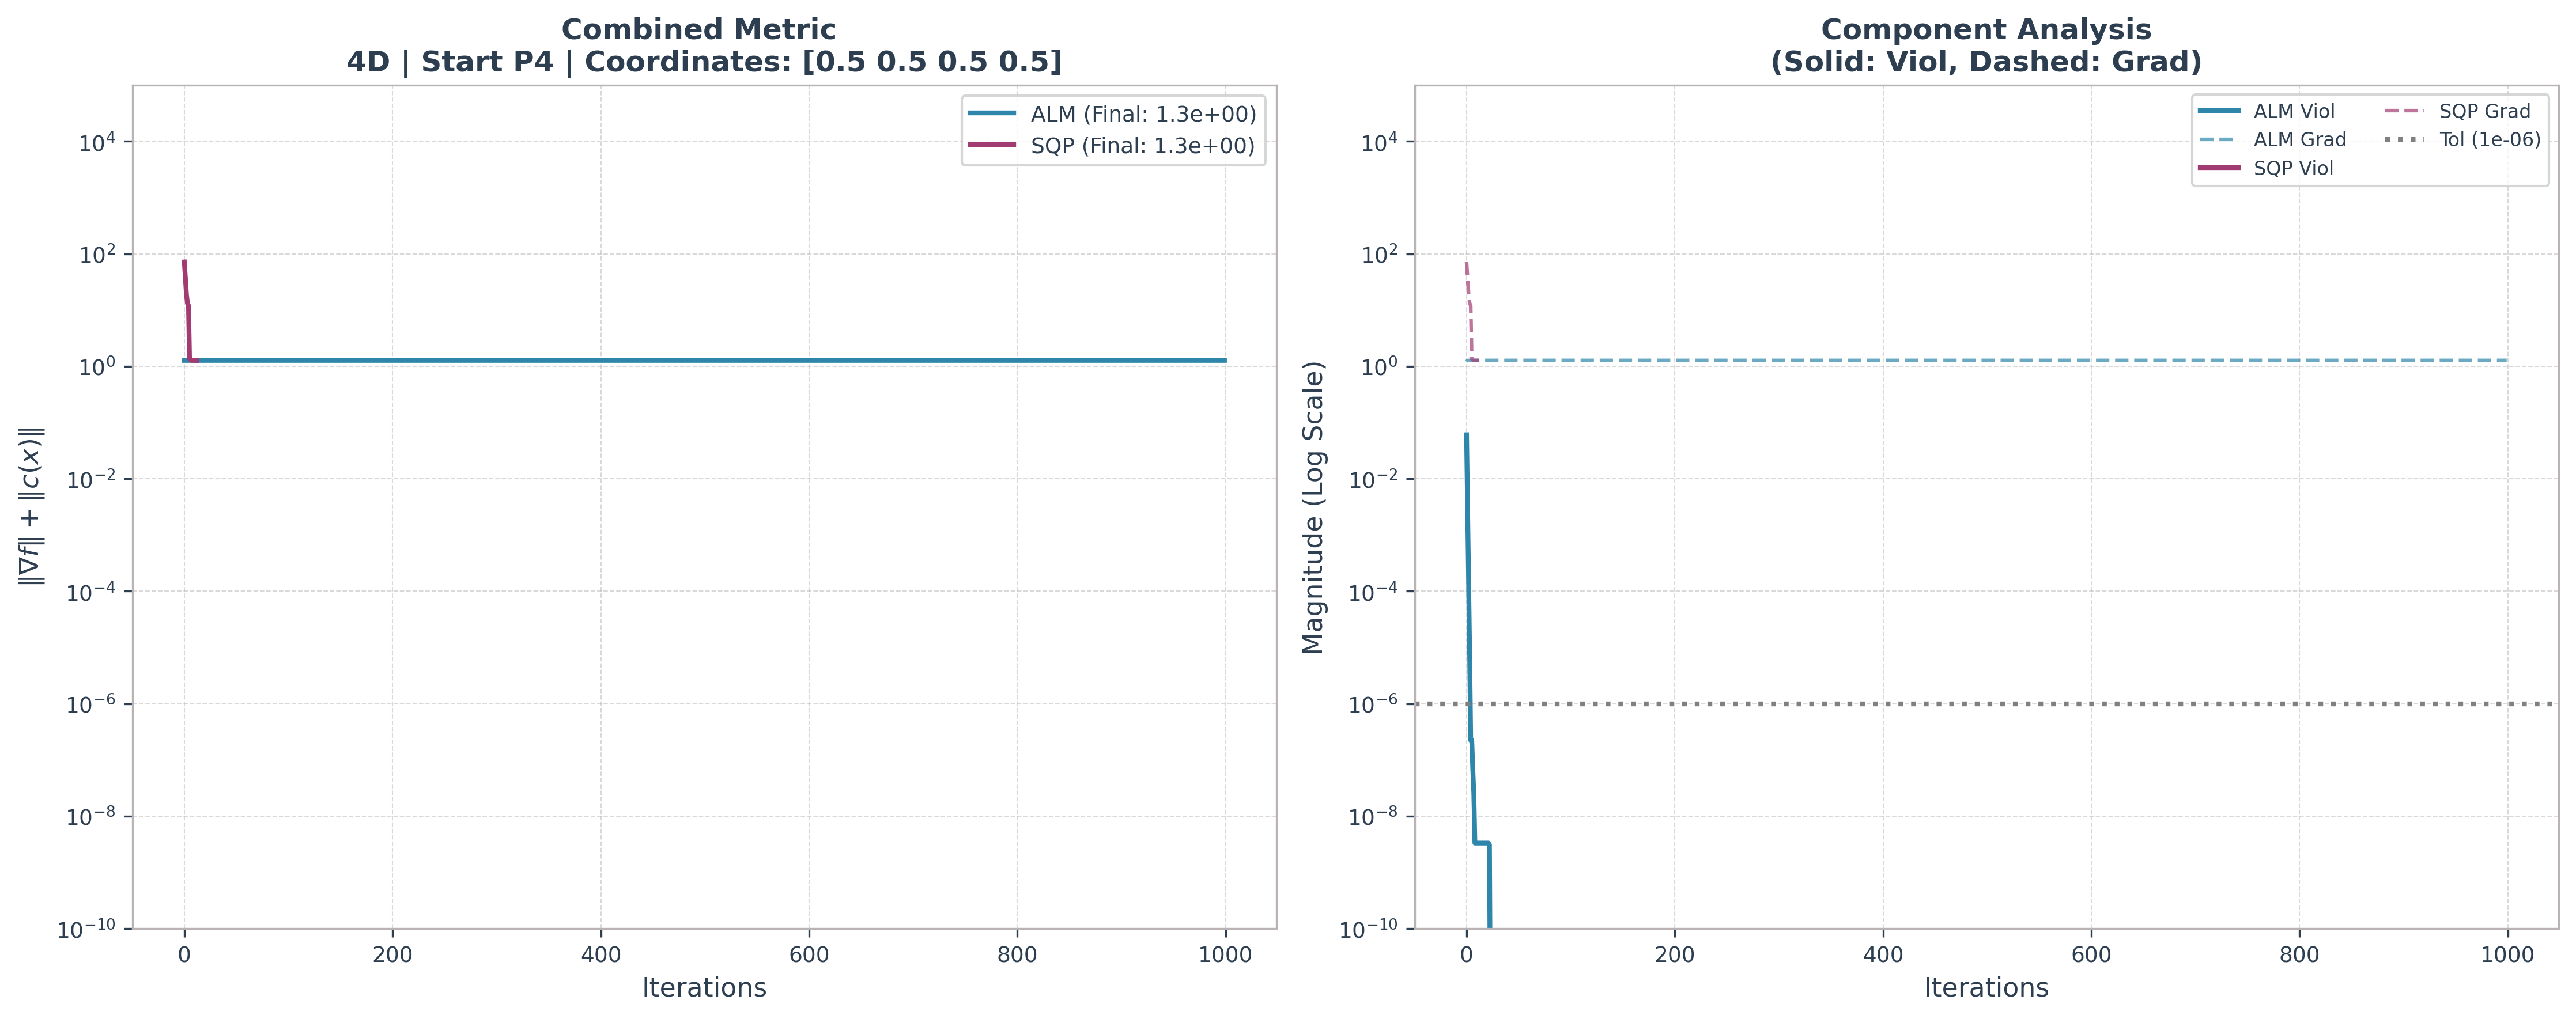
\includegraphics[width=\textwidth]{figures/conv_dual_4D_P4.png}
%         \caption{P4: Start $[0.5, 0.5, 0.5, 0.5]$}
%     \end{subfigure}
    
%     % 这里写主标题
%     \caption{4D Rosenbrock 函数在不同初始点下的收敛曲线对比（P1-P4）。}
%     \label{fig:4d_convergence}
% \end{figure}

% % --- 第二部分：包含 P5 和 P6 ---
% \begin{figure}[H]
%     \ContinuedFloat % <--- 关键命令：告诉 LaTeX 接续上一个 figure 的编号
%     \centering
%     % P5
%     \begin{subfigure}[b]{0.48\textwidth}
%         \centering
%         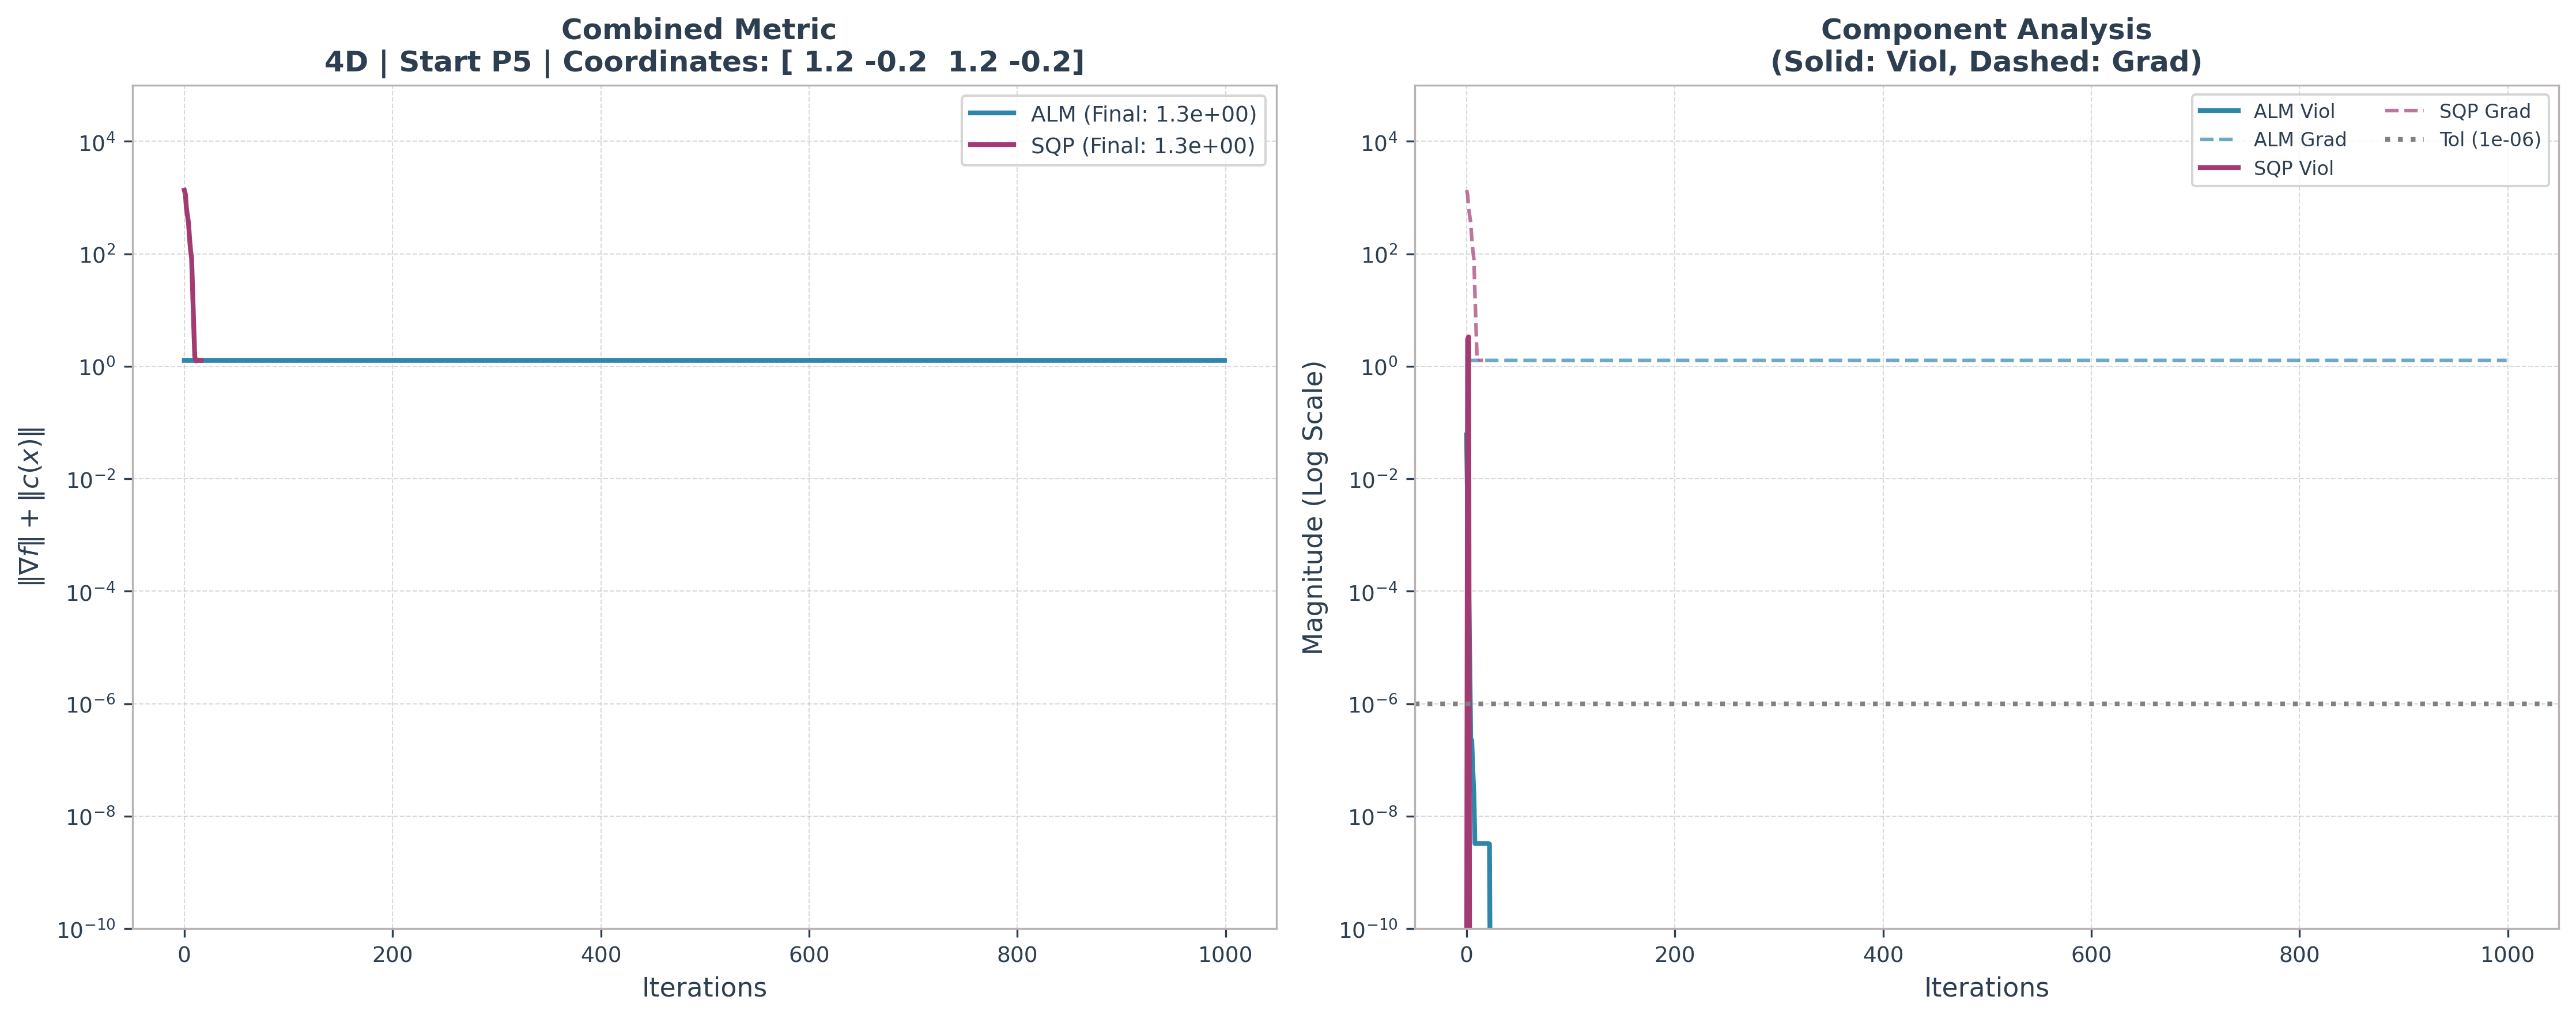
\includegraphics[width=\textwidth]{figures/conv_dual_4D_P5.png}
%         \caption{P5: Start $[1.2, -0.2, 1.2, -0.2]$}
%     \end{subfigure}
%     \hfill
%     % P6
%     \begin{subfigure}[b]{0.48\textwidth}
%         \centering
%         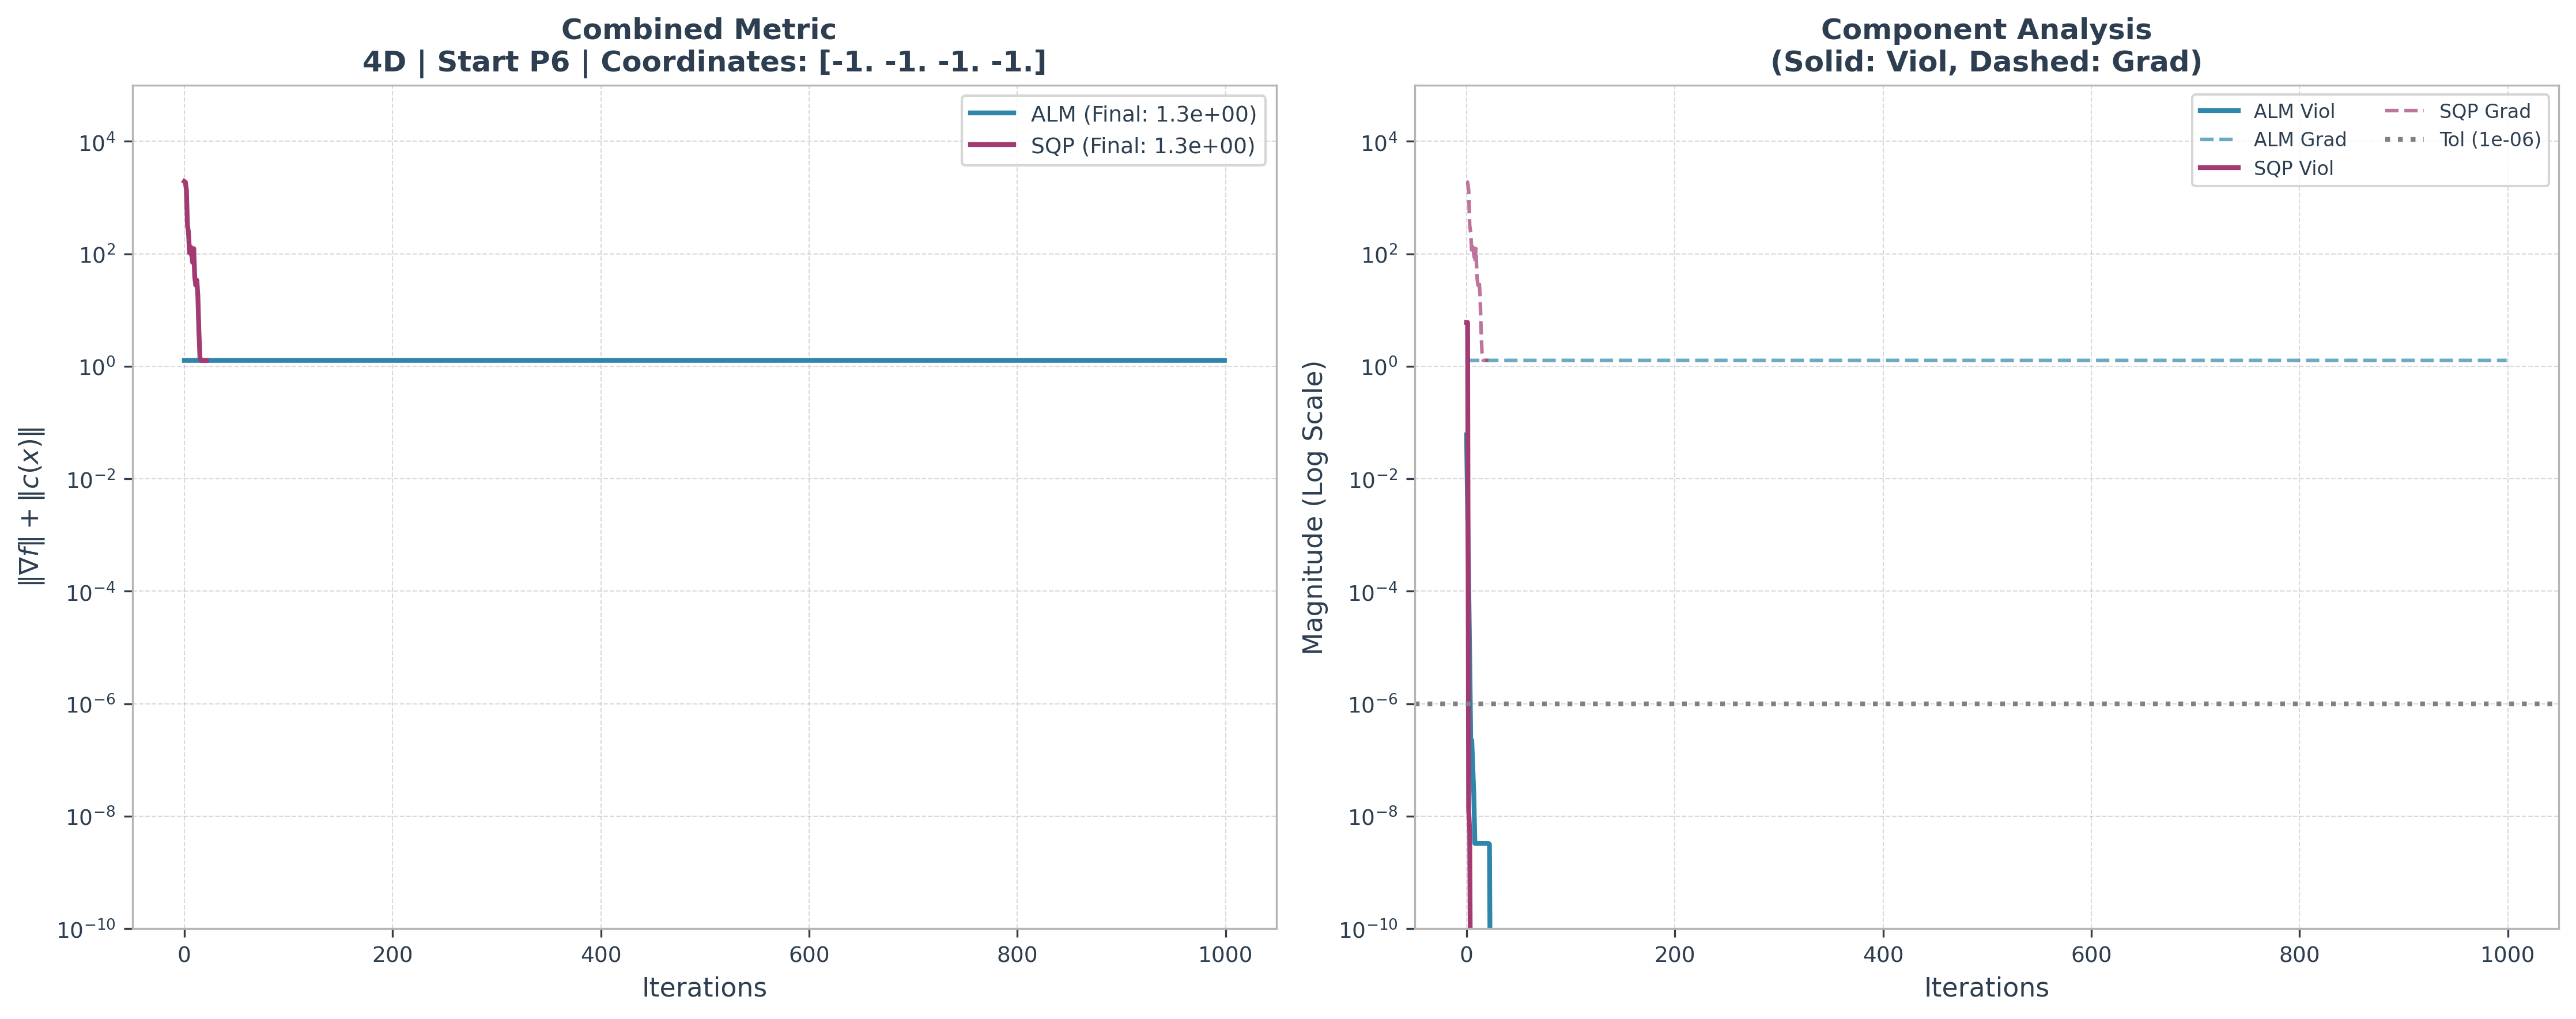
\includegraphics[width=\textwidth]{figures/conv_dual_4D_P6.png}
%         \caption{P6: Start $[-1, -1, -1, -1]$}
%     \end{subfigure}
    
%     % 这里写（续）标题，此时 LaTeX 会自动认为这是 图 X 的继续
%     \caption[]{4D Rosenbrock 函数在不同初始点下的收敛曲线对比（续）。} 
%     \label{fig:4d_convergence_cont}
% \end{figure}

% \mbox{} 用于占据一个不可见的位，\\ 强制换行
\paragraph{结果分析：} \mbox{} \\

综合表 \ref{tab:4d_results} 的数值统计与图 \ref{fig:4d_convergence} 的收敛形态，针对 4D 约束 Rosenbrock 问题的实验结论如下：

\begin{enumerate}
    \item \textbf{边界最优解的 KKT 特征验证：}
    所有测试点的收敛度量最终稳定在 $1.3 \times 10^0$ 量级。分量分析显示，约束违反度迅速降至 $10^{-10}$ 以下（可行），而梯度范数维持在 $\|\nabla f(x^*)\| \approx 1.269$。这严谨地验证了最优解 $x^*$ 位于约束边界上：此时满足 $\nabla f(x^*) + \sum \lambda_i \nabla c_i(x^*) = 0$，目标函数的下降方向被约束梯度的线性组合所平衡，而非内部驻点的零梯度条件。

    \item \textbf{算法机制与效率对比：}
    \begin{itemize}
        \item \textbf{SQP 的子空间优势}：SQP 仅需 13-22 次迭代即可收敛。这得益于其 QP 子问题能精确处理线性约束（$c_1$），使得搜索方向始终沿约束流形的切平面移动，从而避免了锯齿状的修正路径，表现出显著的超线性收敛特性。
        \item \textbf{ALM 的判停准则失配}：ALM 在所有测试中均运行至最大迭代次数（MaxIter）。事实上，其目标函数值早已稳定于 $0.5281$ 且约束满足精度，但由于实验设定的收敛准则为 $\|\nabla f(x)\| \le \epsilon$（仅适用于无约束或内部解），导致算法在已找到边界最优解的情况下，因无法满足梯度消失条件而持续运行。
    \end{itemize}

    \item \textbf{全局收敛鲁棒性：}
    尽管初始点 $P_1-P_6$ 散布于高维空间的不同象限及远场区域，两种算法最终均收敛至同一最优值 $f^* \approx 0.5281$。这表明在该约束限定的可行域内，目标函数呈现出良好的单峰特性，算法对初值变化具有较强的鲁棒性。
\end{enumerate}


\section{思考题}

\subsection{增广拉格朗日法为何比纯罚函数法收敛精度更高？罚参数的选择有何影响？}

\subsubsection{收敛精度与数值稳定性分析}
纯罚函数法与增广拉格朗日法（ALM）虽然均通过构造辅助函数将约束优化转化为无约束优化问题，但二者的收敛机制存在本质差异，这直接决定了其数值精度。

对于纯罚函数法，为了迫使迭代点 $x_k$ 逼近可行域，罚参数 $\mu$ 必须趋于无穷大（$\mu \to \infty$）。然而，随着 $\mu$ 的增大，目标函数的 Hessian 矩阵条件数会急剧增加，导致数值计算出现严重病态（Ill-conditioning）。在这种极度拉伸的几何地貌中，基于梯度的优化算法难以精确定位极小值点，且计算机浮点数截断误差会被放大，从而限制了最终解的精度。

相比之下，增广拉格朗日法在罚函数的基础上引入了拉格朗日乘子项 $\lambda^T c(x)$。根据收敛理论，ALM 并不要求 $\mu \to \infty$，而是通过外层迭代不断更新乘子 $\lambda^{(k)}$ 来逼近最优乘子 $\lambda^*$。只要罚参数 $\mu$ 大于某个有限的阈值，算法即可在 $\mu$ 保持有限值的情况下收敛至满足 KKT 条件的精确解。这种机制避免了海森矩阵的病态化，使得内层子问题求解器（如 BFGS）始终在数值性态良好的曲面上运行，从而获得了显著高于纯罚函数法的收敛精度。

\subsubsection{罚参数 $\mu$ 的灵敏度分析}
罚参数 $\mu$ 的选取需要在收敛速度与数值稳定性之间寻求平衡：
\begin{enumerate}
    \item 若初始 $\mu$ 取值过小或增长缓慢：罚项对约束违反的惩罚力度不足，导致增广拉格朗日函数 $L_A$ 的极小值点远离可行域。这迫使外层循环进行更多次迭代以更新乘子 $\lambda$，显著降低了整体收敛速度。
    \item 若初始 $\mu$ 取值过大或增长过快：虽然能强力抑制约束违反，但会迅速诱发海森矩阵的病态问题。这会导致内层子问题的搜索方向计算误差增大，步长选取困难，甚至导致内层优化算法失效或发散。
\end{enumerate}
因此，工程上通常采用自适应策略，即设定适中的初始值（如 $\mu_0=10$），并仅在约束违反度下降不明显时按比例（如 $\times 5$）增大 $\mu$，以兼顾效率与鲁棒性。

\subsection{序列二次规划（SQP）在处理强非线性约束时表现更优，其核心原因是“二次规划子问题逼近约束优化局部特性”，请结合 2 维测试函数的特点解释这一优势？}

\subsubsection{测试函数的几何特性}
本实验中的 2 维 Rosenbrock 修正函数具有典型的“弯曲峡谷”地貌，目标函数 $f(x)$ 的水平集呈现狭长的香蕉形状。同时，问题包含强非线性等式约束 $c_1(x) = x_1^2 + x_2 - 2 = 0$（抛物线）与线性不等式约束。最优解位于目标函数峡谷底与抛物线约束边界的交汇处。这种“非凸目标函数 + 非凸约束边界”的组合，要求算法必须精确感知约束流形的曲率变化。

\subsubsection{SQP 子问题的几何逼近机制}
SQP 算法在处理此类强非线性问题时表现出优越性，归因于其构造的二次规划（QP）子问题本质上是对 KKT 条件的牛顿法近似：

\begin{enumerate}
    \item 二次模型捕捉曲率信息：在每次迭代点 $x_k$，SQP利用 Hessian 矩阵 $B_k$（通常由 BFGS 更新）构建目标函数的二次近似模型。对于 Rosenbrock 函数，$B_k$ 能够有效捕捉峡谷底部的曲率信息，引导搜索方向沿谷底延伸。
    
    \item 线性化约束定义切空间：SQP 将非线性约束在 $x_k$ 处进行一阶泰勒展开（线性化）：
    \begin{equation}
        c_i(x_k) + \nabla c_i(x_k)^T d = 0
    \end{equation}
    对于抛物线约束 $x_1^2 + x_2 = 2$，线性化过程实际上是在当前点构造了约束流形的切平面（Tangent Plane）。
    
    \item 搜索方向的精确性：QP 子问题的解 $d_k$ 是在切平面上寻找使二次模型下降最快的方向。这意味着 SQP 产生的步长 $d_k$ 既包含了指向目标函数极小值的二阶牛顿方向，又包含了将迭代点拉回约束边界的法向分量。
\end{enumerate}

相比于 ALM 依靠罚项“被动”地将点吸附至边界，SQP 通过求解 QP 子问题，“主动”预测了约束边界的切向走势。这种机制使得 SQP 能够沿着抛物线约束的切线方向大步移动，避免了在峡谷与弯曲边界之间产生锯齿状的震荡路径，从而实现了高效收敛。


\section{实验结论与反思}

\subsection{算法性能对比总结}
本次实验对比了增广拉格朗日法 (ALM) 和序列二次规划法 (SQP) 在求解带强非线性约束（Rosenbrock 函数变体）时的表现。实验数据表明：
\begin{itemize}
    \item \textbf{收敛速度与精度}：SQP 算法展现出显著的优越性，其迭代次数远少于 ALM，且在约束满足精度（Constraint Violation）上能达到 $10^{-9}$ 级别。这归功于 SQP 对非线性约束的局部线性化处理及二阶信息的利用。
    \item \textbf{鲁棒性}：ALM 算法虽然实现逻辑直观，但对罚参数 $\mu$ 的初始值及更新策略较为敏感。在处理抛物线等式约束与峡谷函数交叉的复杂地形时，ALM 容易因罚参数增长导致的数值病态而陷入“迭代上限”或收敛缓慢。
\end{itemize}

\subsection{对收敛准则的思考}
在实验过程中，针对实验要求中给出的收敛准则 $\|\nabla f(x_k)\| \le 10^{-6}$，结合约束优化理论与实际运行结果，我认为：

\subsubsection{目标函数梯度的理论矛盾}
实验要求“同时满足 $\|\nabla f(x_k)\| \le 10^{-6}$ 和 $\|c(x_k)\| \le 10^{-6}$”。从理论上讲，对于约束优化问题，这一要求在最优解位于约束边界上时是不严谨的。
\begin{itemize}
    \item 根据 KKT (Karush-Kuhn-Tucker) 条件，在约束极值点 $x^*$ 处，目标函数的负梯度 $-\nabla f(x^*)$ 应与约束梯度的线性组合平衡，即：
    \begin{equation}
        \nabla f(x^*) + \sum_{i} \lambda_i \nabla c_i(x^*) = 0 \implies \nabla f(x^*) = - \sum_{i} \lambda_i \nabla c_i(x^*)
    \end{equation}
    \item 这意味着，只要拉格朗日乘子 $\lambda_i \neq 0$（即约束是起作用的/Active的），目标函数的梯度 $\nabla f(x^*)$ 通常不为 0。
    \item \textbf{实验证据}：在本次实验的 SQP 算法运行结果中，我们观察到某些收敛点的约束违反度极低（$\|c(x)\| < 10^{-8}$），但此时 $\|\nabla f(x)\|$ 约为 $2.23$。这证实了最优解位于约束边界上，此时 $\nabla f$ 被非零的约束力所抵消，而非趋于零。
\end{itemize}

\subsubsection{对收敛准则的修正理解}
基于上述分析，我认为实验要求中的 $\|\nabla f(x_k)\| \le 10^{-6}$ 应在不同算法背景下有不同的理解：
\begin{itemize}
    \item \textbf{对于 ALM 算法}：ALM 的内层循环是求解无约束子问题 $\min L_A(x, \lambda, \mu)$。这里的梯度要求应理解为增广拉格朗日函数的梯度趋于 0，即 $\|\nabla L_A(x_k)\| \le 10^{-6}$，而非原始目标函数 $\nabla f$。代码实现中若直接使用 $\nabla f$ 作为内层终止条件会导致逻辑错误。
    \item \textbf{对于 SQP 算法}：收敛的实质是拉格朗日函数的梯度趋于 0（$\|\nabla \mathcal{L}\| \to 0$）以及搜索方向 $d_k \to 0$。若严格按照实验要求 $\|\nabla f\| \to 0$，会导致算法在边界最优解处被错误地判定为“未收敛”，这也是SQP问题一直未收敛的重要原因。
\end{itemize}

\textbf{改进建议}：在未来的实验或实际工程应用中，更科学的收敛准则应是检查 KKT 残差 (KKT Residual)，即同时检查可行性 $\|c(x)\|$ 和拉格朗日梯度的平稳性 $\|\nabla f(x) + \lambda^T \nabla c(x)\|$。

\subsection{总结}
综上所述，本次实验不仅验证了 SQP 在处理强非线性约束问题上的高效性，也加深了我对约束优化几何意义及 KKT 条件的理解。特别是在代码实现环节，如何正确处理“边界最优解”时的梯度判定，是连接理论与实践的关键一环。



% \begin{thebibliography}{99}
% \bibitem{ref1} Nocedal, J., \& Wright, S. J. (2006). \textit{Numerical Optimization}. Springer Science \& Business Media.
% \bibitem{ref2} 陈宝林. (2005). \textit{最优化理论与算法}. 清华大学出版社.
% \bibitem{ref3} Powell, M. J. D. (1978). \textit{A Fast Algorithm for Nonlinearly Constrained Optimization Calculations}. Numerical Analysis.
% \end{thebibliography}
\begin{thebibliography}{99}

% 书籍：Author, A. A. (Year). Title of work. Publisher.
\bibitem{ref1} Nocedal, J., \& Wright, S. J. (2006). \textit{Numerical optimization} (2nd ed.). Springer.

% 中文书籍：作者. (年份). 书名. 出版社.
\bibitem{ref2} 陈宝林. (2005). \textit{最优化理论与算法} (第2版). 清华大学出版社.

% 论文集/章节：Author, A. A. (Year). Title of chapter. In Editor (Ed.), Title of book (pp. xx-xx). Publisher.
% Powell 这篇通常收录在 Lecture Notes in Mathematics 丛书中
\bibitem{ref3} Powell, M. J. D. (1978). A fast algorithm for nonlinearly constrained optimization calculations. In G. A. Watson (Ed.), \textit{Numerical analysis} (pp. 144--157). Springer.

\end{thebibliography}
% --- 正文结束 ---

\clearpage % 强制换页，让附录从新的一页开始

\appendix % 开启附录模式，章节编号变为 A, B...

% --- 以下设置用于将图表编号改为 A.1, A.2 的格式 ---
\renewcommand{\thetable}{\thesection.\arabic{table}}
\renewcommand{\thefigure}{\thesection.\arabic{figure}}


\section{详细实验数据记录} \label{app:data}
\setcounter{table}{0}
\setcounter{figure}{0}

本附录汇总了 10 组不同初始点（$P_1 - P_{10}$）下，ALM 与 SQP 算法在 2D 及 4D 测试问题中的完整迭代数据。

\subsection{初始点定义}
表 \ref{tab:start_points} 列出了所有测试用例的初始坐标配置。

\begin{table}[H]
    \centering
    \caption{测试问题初始点坐标定义 ($P_1 - P_{10}$)}
    \label{tab:start_points}
    \footnotesize
    \begin{tabular}{cll}
        \toprule
        \textbf{Point ID} & \textbf{2D Coordinates} $(x_1, x_2)$ & \textbf{4D Coordinates} $(x_1, x_2, x_3, x_4)$ \\
        \midrule
        $P_1$ & $[-1.2, 1.0]$ & $[0, 0, 0, 0]$ \\
        $P_2$ & $[1.5, 2.5]$  & $[1, 1, 1, 1]$ \\
        $P_3$ & $[0.0, 0.0]$  & $[-0.5, 0.5, -0.5, 0.5]$ \\
        $P_4$ & $[-1.4, -0.4]$& $[0.5, 0.5, 0.5, 0.5]$ \\
        $P_5$ & $[1.8, 0.5]$  & $[1.2, -0.2, 1.2, -0.2]$ \\
        $P_6$ & $[0.5, 2.8]$  & $[-1, -1, -1, -1]$ \\
        $P_7$ & $[1.0, 1.0]$  & $[2, 0, 0, 0]$ \\
        $P_8$ & $[-1.5, 3.0]$ & $[0.1, 0.1, 0.1, 0.1]$ \\
        $P_9$ & $[0.0, 2.0]$  & $[3, 3, 3, 3]$ \\
        $P_{10}$ & $[2.0, -0.5]$& $[-1, 2, -1, 2]$ \\
        \bottomrule
    \end{tabular}
\end{table}

\subsection{2D Modified Rosenbrock 测试结果}
表 \ref{tab:full_results_2d} 展示了二维问题下的详细性能指标。需注意，SQP 算法在 $P_3, P_5, P_6, P_7, P_{10}$ 能够收敛至严格满足 KKT 条件的内部解或精确边界解（Success），而在其他点则收敛于边界（Boundary）。


% ==========================================
% 表 1: 2D 问题实验结果
% ==========================================
\begin{table}[H]
    \centering
    \caption{2D 测试问题完整实验结果统计}
    \label{tab:full_results_2d}
    \scriptsize 
    \setlength{\tabcolsep}{3.5pt} 
    \begin{tabular}{clc c ccc l}
        \toprule
        \textbf{ID} & \textbf{Algo} & \textbf{Iter} & \textbf{Final } $\mathbf{x}$ & \textbf{Final } $f(x)$ & \textbf{Viol.} $\|c(x)\|$ & \textbf{Grad} $\|\nabla f\|$ & \textbf{Status} \\
        \midrule
        
        % P1
        \multirow{2}{*}{$P_1$} 
        & ALM & 1000 & $(-0.999, 1.002)$ & 3.9980 & $3.27 \times 10^{-10}$ & 2.236 & MaxIter \\
        & SQP & 6    & $(-0.999, 1.002)$ & 3.9980 & $1.57 \times 10^{-11}$ & 2.235 & Boundary \\ \cmidrule{1-8}
        
        % P2
        \multirow{2}{*}{$P_2$} 
        & ALM & 1000 & $(1.000, 1.000)$ & $8.88 \times 10^{-11}$ & $1.61 \times 10^{-11}$ & $3.66 \times 10^{-4}$ & MaxIter \\
        & SQP & 8    & $(1.000, 1.000)$ & $1.20 \times 10^{-15}$ & $3.69 \times 10^{-13}$ & $1.35 \times 10^{-6}$ & Boundary \\ \cmidrule{1-8}

        % P3
        \multirow{2}{*}{$P_3$} 
        & ALM & 1000 & $(-0.999, 1.002)$ & 3.9980 & $1.00 \times 10^{-10}$ & 2.237 & MaxIter \\
        & SQP & 2    & $(1.000, 1.000)$ & $3.00 \times 10^{-31}$ & 0.0 & $1.09 \times 10^{-14}$ & Success \\ \cmidrule{1-8}

        % P4
        \multirow{2}{*}{$P_4$} 
        & ALM & 1000 & $(-0.999, 1.002)$ & 3.9980 & $5.19 \times 10^{-12}$ & 2.236 & MaxIter \\
        & SQP & 7    & $(-0.999, 1.002)$ & 3.9980 & $1.50 \times 10^{-11}$ & 2.235 & Boundary \\ \cmidrule{1-8}

        % P5
        \multirow{2}{*}{$P_5$} 
        & ALM & 1000 & $(1.000, 1.000)$ & $5.73 \times 10^{-10}$ & $2.78 \times 10^{-11}$ & $9.30 \times 10^{-4}$ & MaxIter \\
        & SQP & 8    & $(1.000, 1.000)$ & $1.13 \times 10^{-17}$ & $6.75 \times 10^{-10}$ & $7.12 \times 10^{-8}$ & Success \\ \cmidrule{1-8}

        % P6
        \multirow{2}{*}{$P_6$} 
        & ALM & 1000 & $(1.000, 1.000)$ & $5.77 \times 10^{-10}$ & $9.70 \times 10^{-11}$ & $9.33 \times 10^{-4}$ & MaxIter \\
        & SQP & 9    & $(1.000, 1.000)$ & $8.60 \times 10^{-19}$ & $1.22 \times 10^{-13}$ & $3.60 \times 10^{-8}$ & Success \\ \cmidrule{1-8}

        % P7
        \multirow{2}{*}{$P_7$} 
        & ALM & 1    & $(1.000, 1.000)$ & $3.00 \times 10^{-31}$ & 0.0 & $1.09 \times 10^{-14}$ & Success \\
        & SQP & 1    & $(1.000, 1.000)$ & $3.00 \times 10^{-31}$ & 0.0 & $1.09 \times 10^{-14}$ & Success \\ \cmidrule{1-8}

        % P8
        \multirow{2}{*}{$P_8$} 
        & ALM & 1000 & $(-0.999, 1.002)$ & 3.9980 & $6.48 \times 10^{-10}$ & 2.237 & MaxIter \\
        & SQP & 8    & $(-0.999, 1.002)$ & 3.9980 & $1.11 \times 10^{-14}$ & 2.235 & Boundary \\ \cmidrule{1-8}

        % P9
        \multirow{2}{*}{$P_9$} 
        & ALM & 1000 & $(-0.999, 1.002)$ & 3.9980 & $3.13 \times 10^{-10}$ & 2.237 & MaxIter \\
        & SQP & 8    & $(-0.999, 1.002)$ & 3.9980 & $1.33 \times 10^{-12}$ & 2.235 & Boundary \\ \cmidrule{1-8}

        % P10
        \multirow{2}{*}{$P_{10}$} 
        & ALM & 1000 & $(1.000, 1.000)$ & $4.75 \times 10^{-10}$ & $2.95 \times 10^{-11}$ & $8.47 \times 10^{-4}$ & MaxIter \\
        & SQP & 7    & $(1.000, 1.000)$ & $2.52 \times 10^{-17}$ & $6.59 \times 10^{-13}$ & $1.95 \times 10^{-7}$ & Success \\
        \bottomrule
    \end{tabular}

     {\footnotesize \begin{flushleft}
    注：\textbf{Status} 定义：\textbf{Boundary} (ConvergedOnBoundary) 表示收敛至边界；\textbf{MaxIter} 表示达到最大迭代次数；\textbf{Success} 表示无约束或完全满足精度的收敛。
    \end{flushleft}}
\end{table}


\subsection{4D Constrained Rosenbrock 测试结果}
表 \ref{tab:full_results_4d} 汇总了四维高难度约束问题的数据。所有测试点均收敛至同一边界最优解 $f(x) \approx 0.5281$。

% ==========================================
% 表 2: 4D 问题实验结果
% ==========================================
\begin{table}[H]
    \centering
    \caption{4D 测试问题完整实验结果统计}
    \label{tab:full_results_4d}
    \scriptsize 
    \setlength{\tabcolsep}{3pt} 
    \begin{tabular}{clc c ccc l}
        \toprule
        \textbf{ID} & \textbf{Algo} & \textbf{Iter} & \textbf{Final } $\mathbf{x}$ {\tiny (rounded)} & \textbf{Final } $f(x)$ & \textbf{Viol.} $\|c(x)\|$ & \textbf{Grad} $\|\nabla f\|$ & \textbf{Status} \\
        \midrule
        
        % P1
        \multirow{2}{*}{$P_1$} 
        & ALM & 1000 & $(0.797, 0.636, 0.405, 0.161)$ & 0.5281 & $5.81 \times 10^{-12}$ & 1.269 & MaxIter \\
        & SQP & 16   & $(0.797, 0.636, 0.405, 0.161)$ & 0.5281 & 0.0 & 1.269 & Boundary \\ \cmidrule{1-8}

        % P2
        \multirow{2}{*}{$P_2$} 
        & ALM & 1000 & $(0.797, 0.636, 0.405, 0.161)$ & 0.5281 & $3.38 \times 10^{-12}$ & 1.269 & MaxIter \\
        & SQP & 15   & $(0.797, 0.636, 0.405, 0.161)$ & 0.5281 & 0.0 & 1.269 & Boundary \\ \cmidrule{1-8}

        % P3
        \multirow{2}{*}{$P_3$} 
        & ALM & 1000 & $(0.797, 0.636, 0.405, 0.161)$ & 0.5281 & $1.08 \times 10^{-12}$ & 1.269 & MaxIter \\
        & SQP & 16   & $(0.797, 0.636, 0.405, 0.161)$ & 0.5281 & 0.0 & 1.269 & Boundary \\ \cmidrule{1-8}

        % P4
        \multirow{2}{*}{$P_4$} 
        & ALM & 1000 & $(0.797, 0.636, 0.405, 0.161)$ & 0.5281 & $3.38 \times 10^{-12}$ & 1.269 & MaxIter \\
        & SQP & 13   & $(0.797, 0.636, 0.405, 0.161)$ & 0.5281 & 0.0 & 1.269 & Boundary \\ \cmidrule{1-8}

        % P5
        \multirow{2}{*}{$P_5$} 
        & ALM & 1000 & $(0.797, 0.636, 0.405, 0.161)$ & 0.5281 & $5.91 \times 10^{-12}$ & 1.269 & MaxIter \\
        & SQP & 17   & $(0.797, 0.636, 0.405, 0.161)$ & 0.5281 & $2.22 \times 10^{-16}$ & 1.269 & Boundary \\ \cmidrule{1-8}

        % P6
        \multirow{2}{*}{$P_6$} 
        & ALM & 1000 & $(0.797, 0.636, 0.405, 0.161)$ & 0.5281 & $2.97 \times 10^{-12}$ & 1.269 & MaxIter \\
        & SQP & 22   & $(0.797, 0.636, 0.405, 0.161)$ & 0.5281 & $2.22 \times 10^{-16}$ & 1.269 & Boundary \\ \cmidrule{1-8}

        % P7
        \multirow{2}{*}{$P_7$} 
        & ALM & 1000 & $(0.797, 0.636, 0.405, 0.161)$ & 0.5281 & $4.21 \times 10^{-12}$ & 1.269 & MaxIter \\
        & SQP & 18   & $(0.797, 0.636, 0.405, 0.161)$ & 0.5281 & 0.0 & 1.269 & Boundary \\ \cmidrule{1-8}

        % P8
        \multirow{2}{*}{$P_8$} 
        & ALM & 1000 & $(0.797, 0.636, 0.405, 0.161)$ & 0.5281 & $3.74 \times 10^{-12}$ & 1.269 & MaxIter \\
        & SQP & 13   & $(0.797, 0.636, 0.405, 0.161)$ & 0.5281 & 0.0 & 1.269 & Boundary \\ \cmidrule{1-8}

        % P9
        \multirow{2}{*}{$P_9$} 
        & ALM & 1000 & $(0.797, 0.636, 0.405, 0.161)$ & 0.5281 & $3.46 \times 10^{-12}$ & 1.269 & MaxIter \\
        & SQP & 22   & $(0.797, 0.636, 0.405, 0.161)$ & 0.5281 & $2.22 \times 10^{-16}$ & 1.269 & Boundary \\ \cmidrule{1-8}

        % P10
        \multirow{2}{*}{$P_{10}$} 
        & ALM & 1000 & $(0.797, 0.636, 0.405, 0.161)$ & 0.5281 & $2.00 \times 10^{-12}$ & 1.269 & MaxIter \\
        & SQP & 18   & $(0.797, 0.636, 0.405, 0.161)$ & 0.5281 & 0.0 & 1.269 & Boundary \\
        \bottomrule
    \end{tabular}
\end{table}



\clearpage
\section{补充可视化图表} \label{app:plots}
\setcounter{figure}{0} % 重置图片计数器，编号变为 B.1, B.2...
\renewcommand{\thefigure}{\thesection.\arabic{figure}}

本附录提供了实验的完整可视化记录，包括迭代次数统计概览、收敛曲线网格图以及 2D 测试的所有迭代路径详情。

\subsection{2D 问题可视化分析}

图 \ref{fig:app_summary_2d} 展示了不同初始点下 ALM 与 SQP 的迭代效率对比，图 \ref{fig:app_conv_grid_2d} 则展示了所有测试点的收敛曲线。图 \ref{fig:app_all_paths} 详细描绘了从 $P_1$ 到 $P_{10}$ 的完整搜索路径。

% --- 1. 2D 迭代次数概览图 ---
\begin{figure}[hbt!]
    \centering
    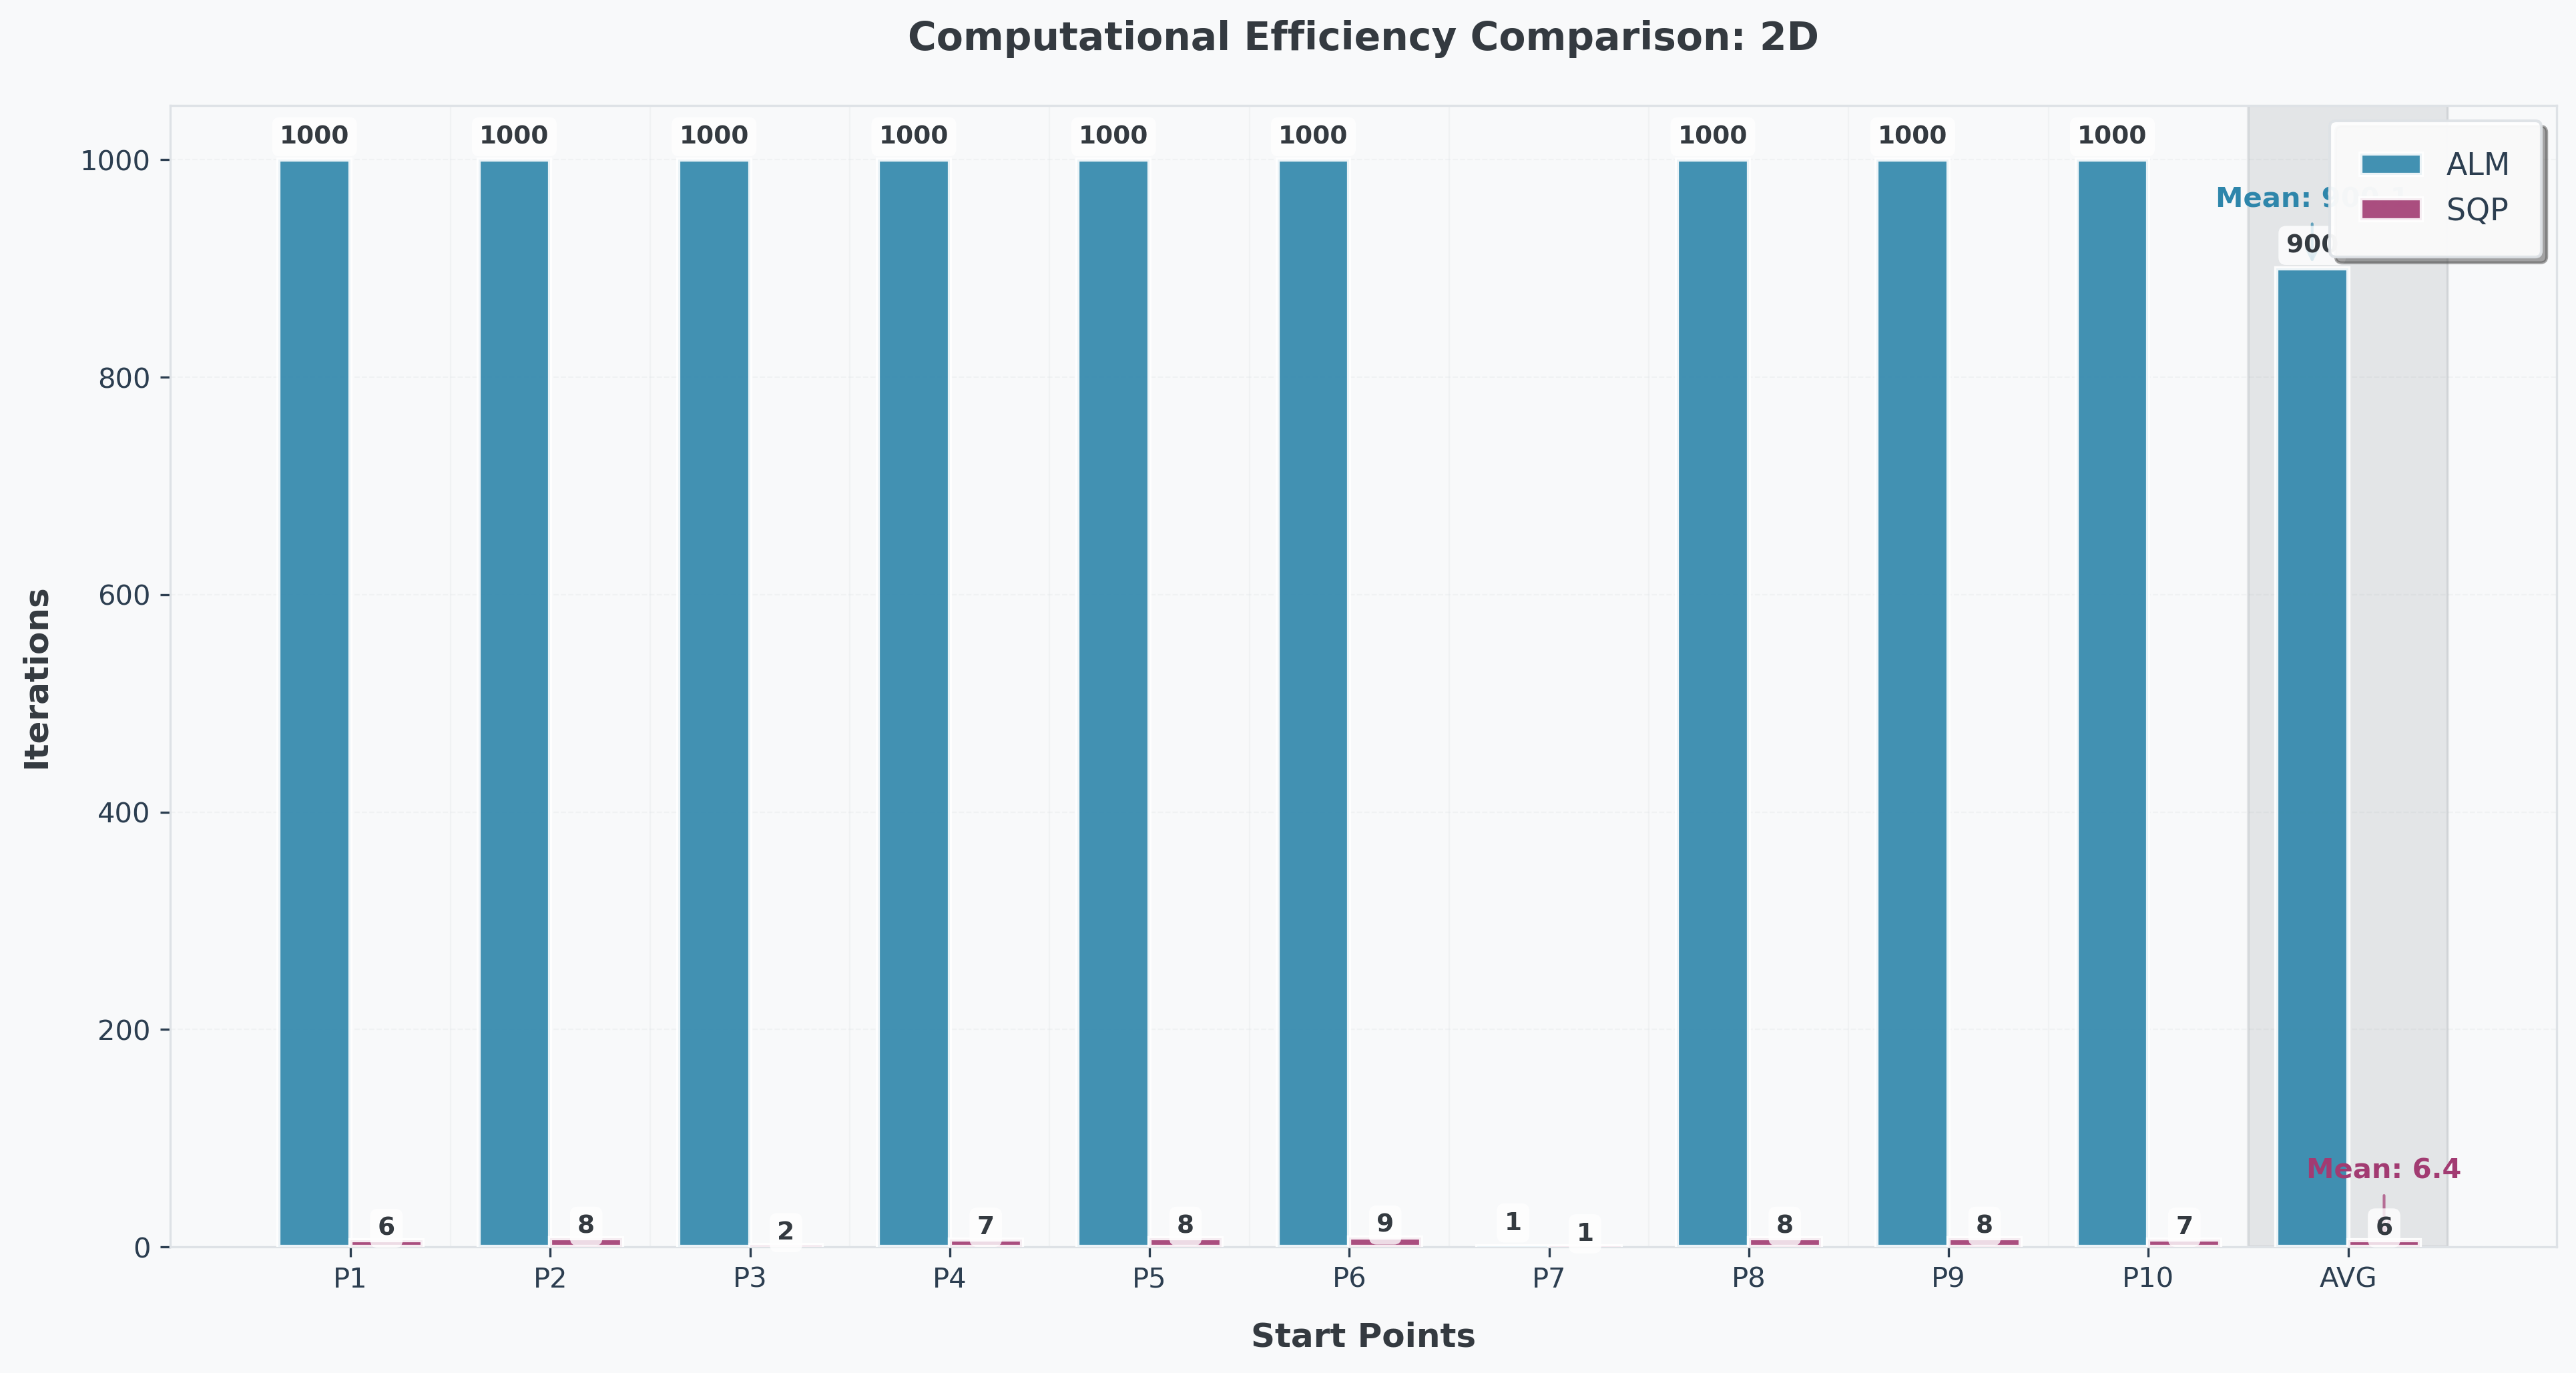
\includegraphics[width=0.9\textwidth]{figures/summary_2D.png} % 请替换实际文件名
    \caption{2D 测试问题：不同初始点下的迭代次数 (Iterations) 对比统计}
    \label{fig:app_summary_2d}
\end{figure}

% --- 2. 2D 收敛曲线网格图 ---
\begin{figure}[hbt!]
    \centering
    % 关键修改：增加 height 和 keepaspectratio 参数
    % height=0.9\textheight 表示高度最多占版面的 90%
    % width=1.0\textwidth 表示宽度最多占 100%
    % keepaspectratio 保证图片不变形，自动选择较小的那个缩放比例
    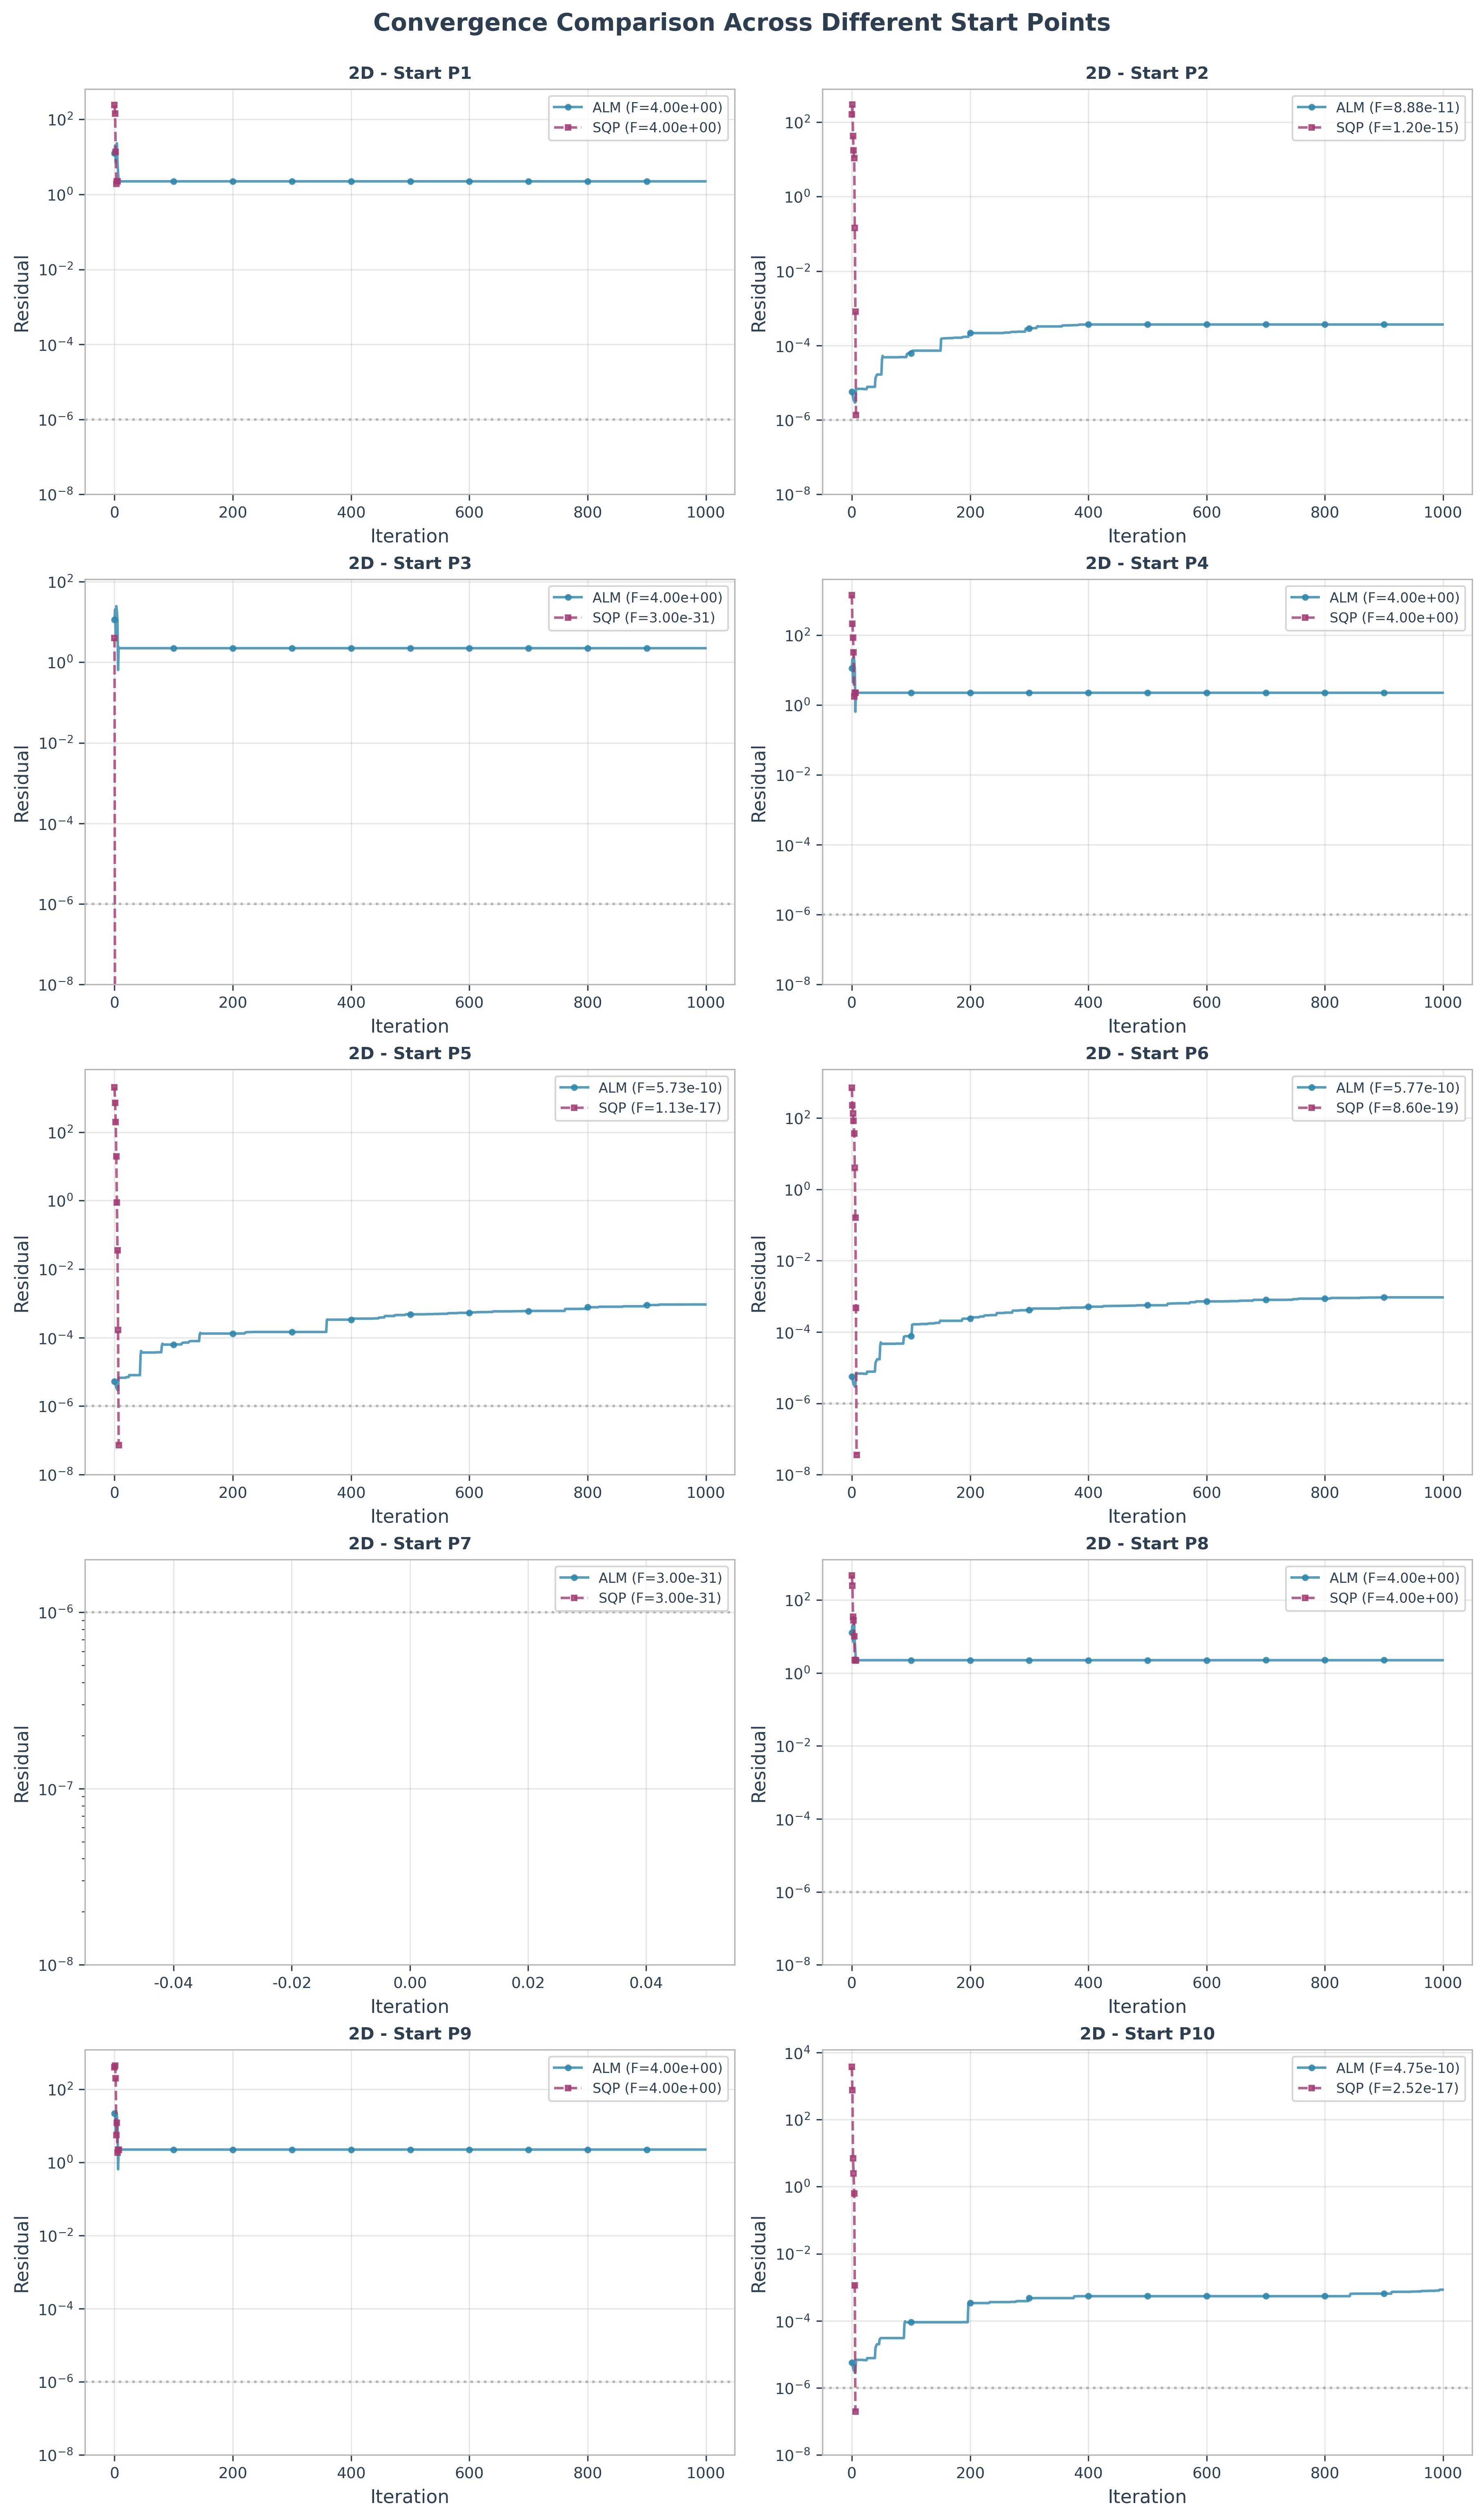
\includegraphics[width=1.0\textwidth, height=0.9\textheight, keepaspectratio]{figures/convergence_grid_comparison_2D.png}
    \caption{2D 测试问题：所有初始点的 KKT 误差收敛曲线网格图}
    \label{fig:app_conv_grid_2d}
\end{figure}

% \begin{figure}[p] % [p] 表示强制单独成页，适合这种大组图
%     \centering
%     % 第一行
%     \begin{subfigure}[b]{0.48\textwidth}
%         \centering
%         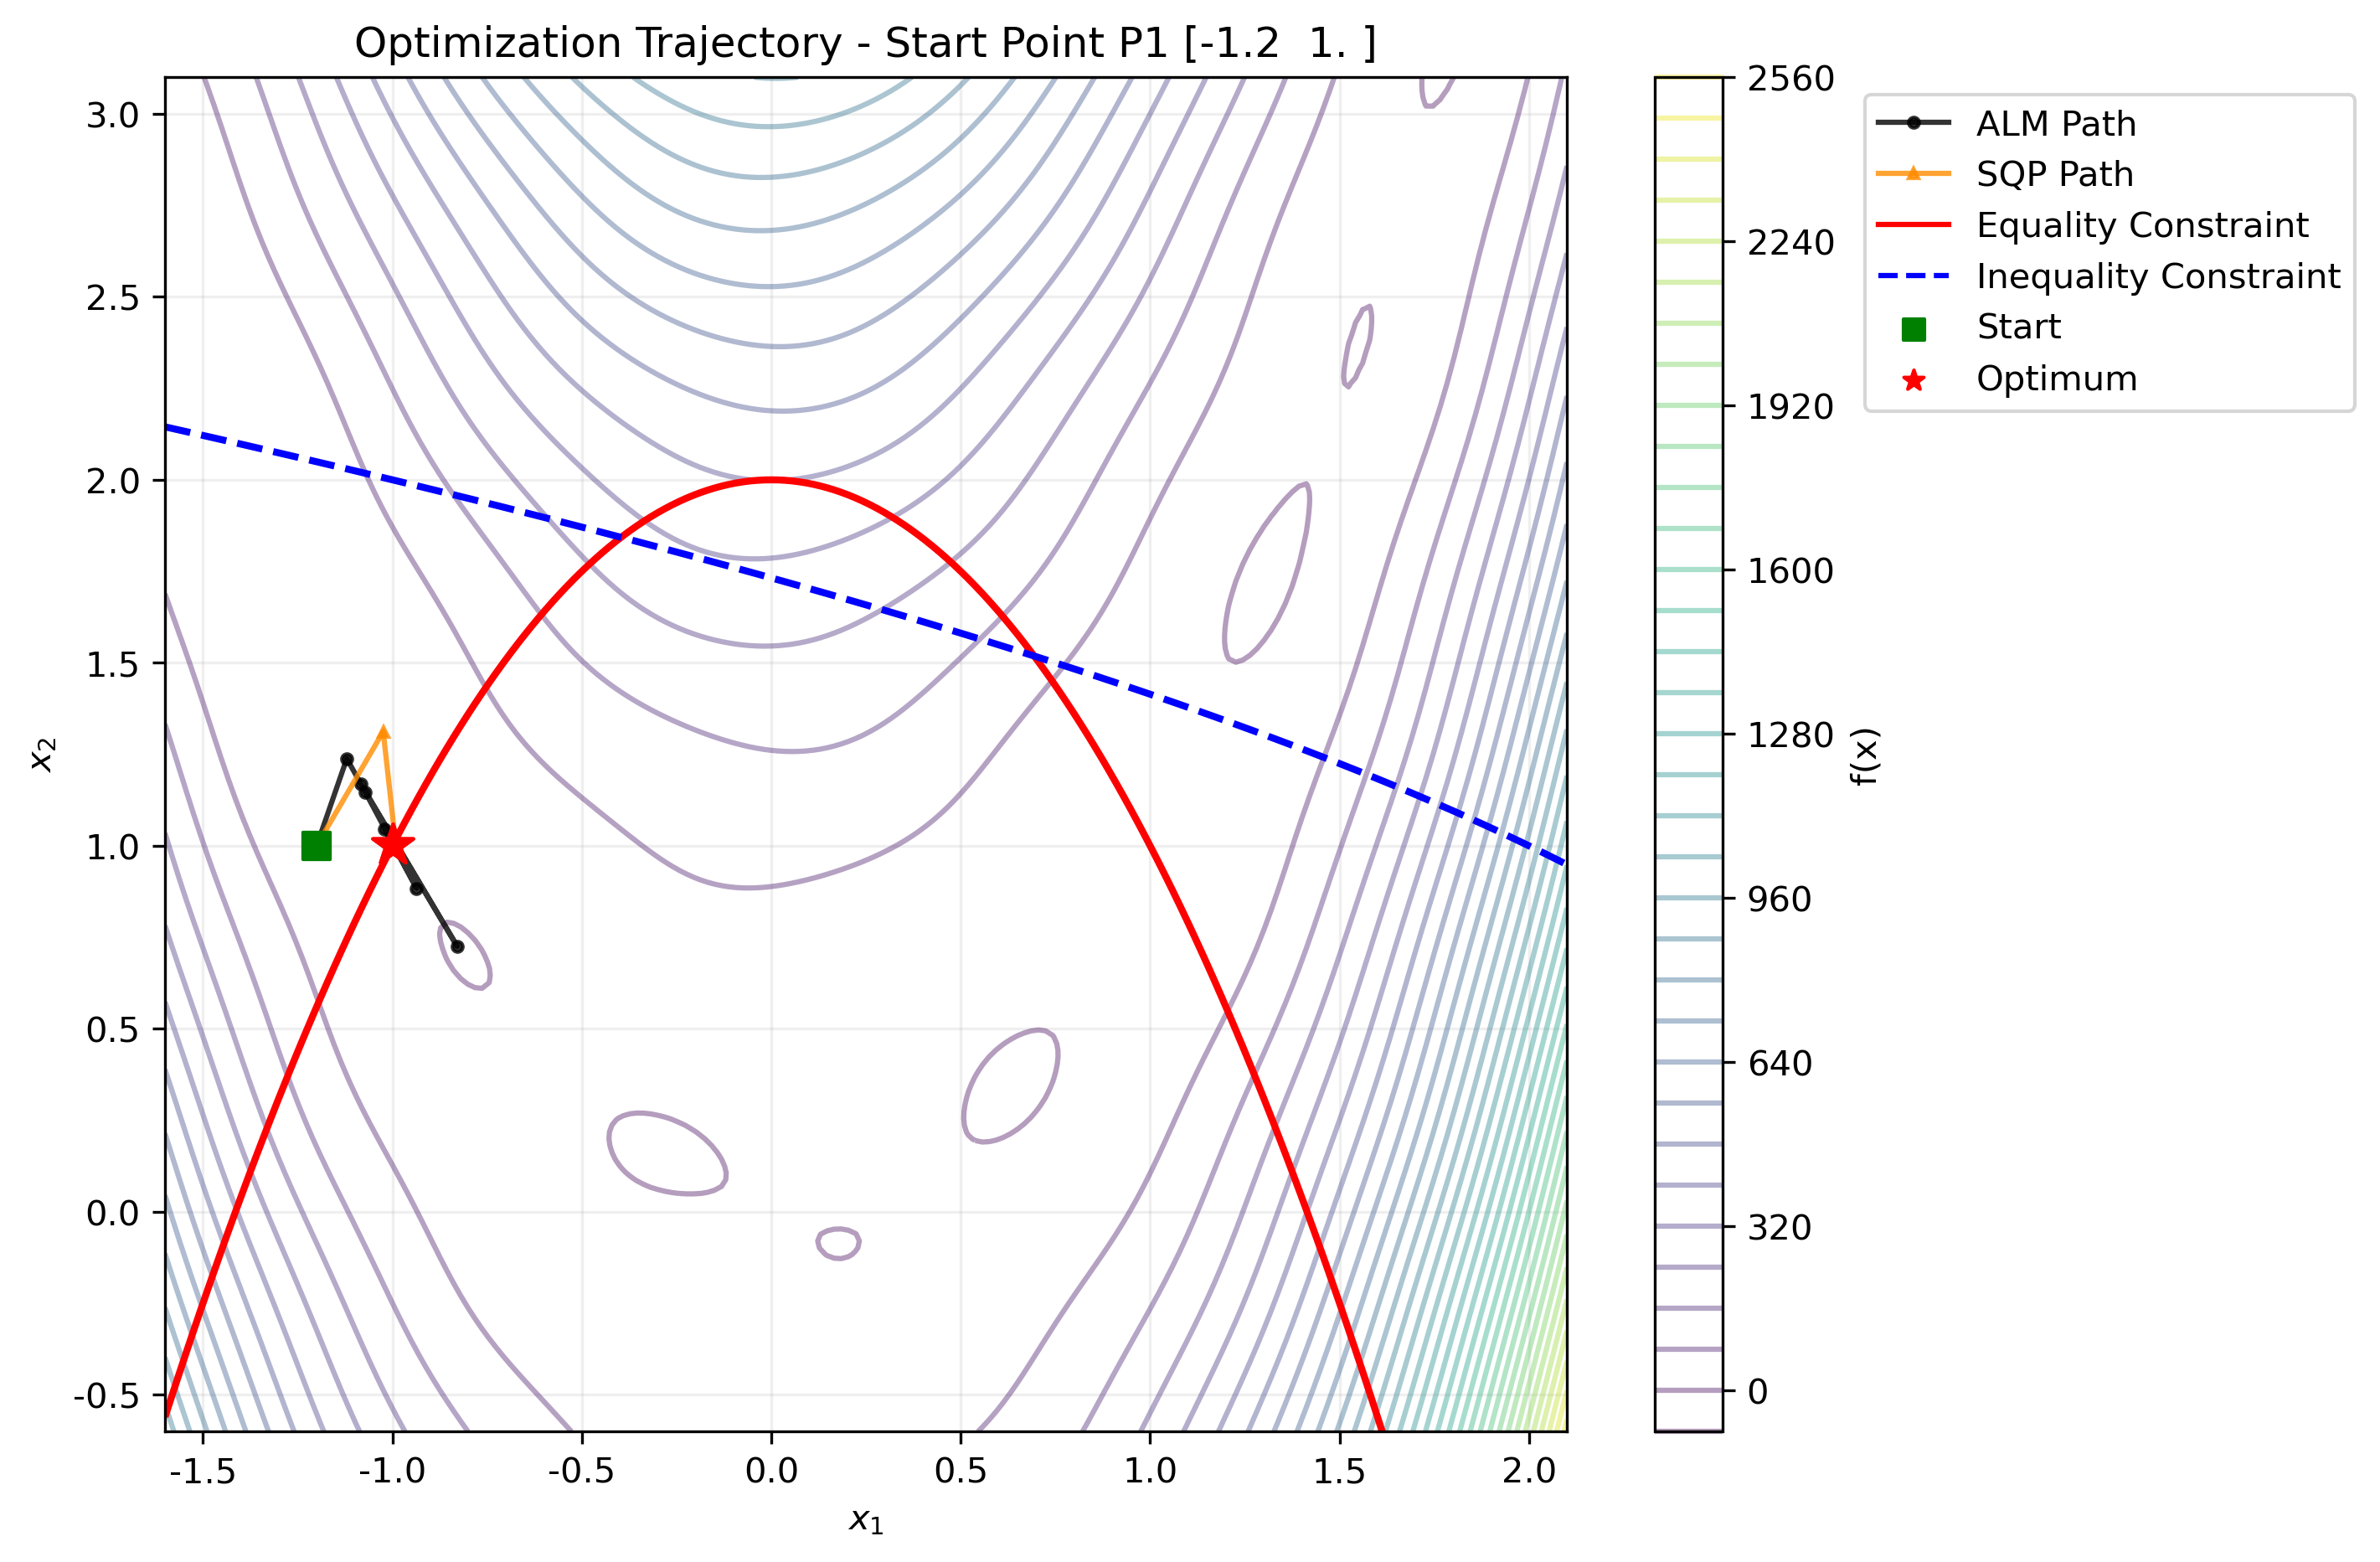
\includegraphics[width=\textwidth]{figures/path_2D_P1.png}
%         \caption{$P_1$: Left Local Min}
%     \end{subfigure}
%     \hfill
%     \begin{subfigure}[b]{0.48\textwidth}
%         \centering
%         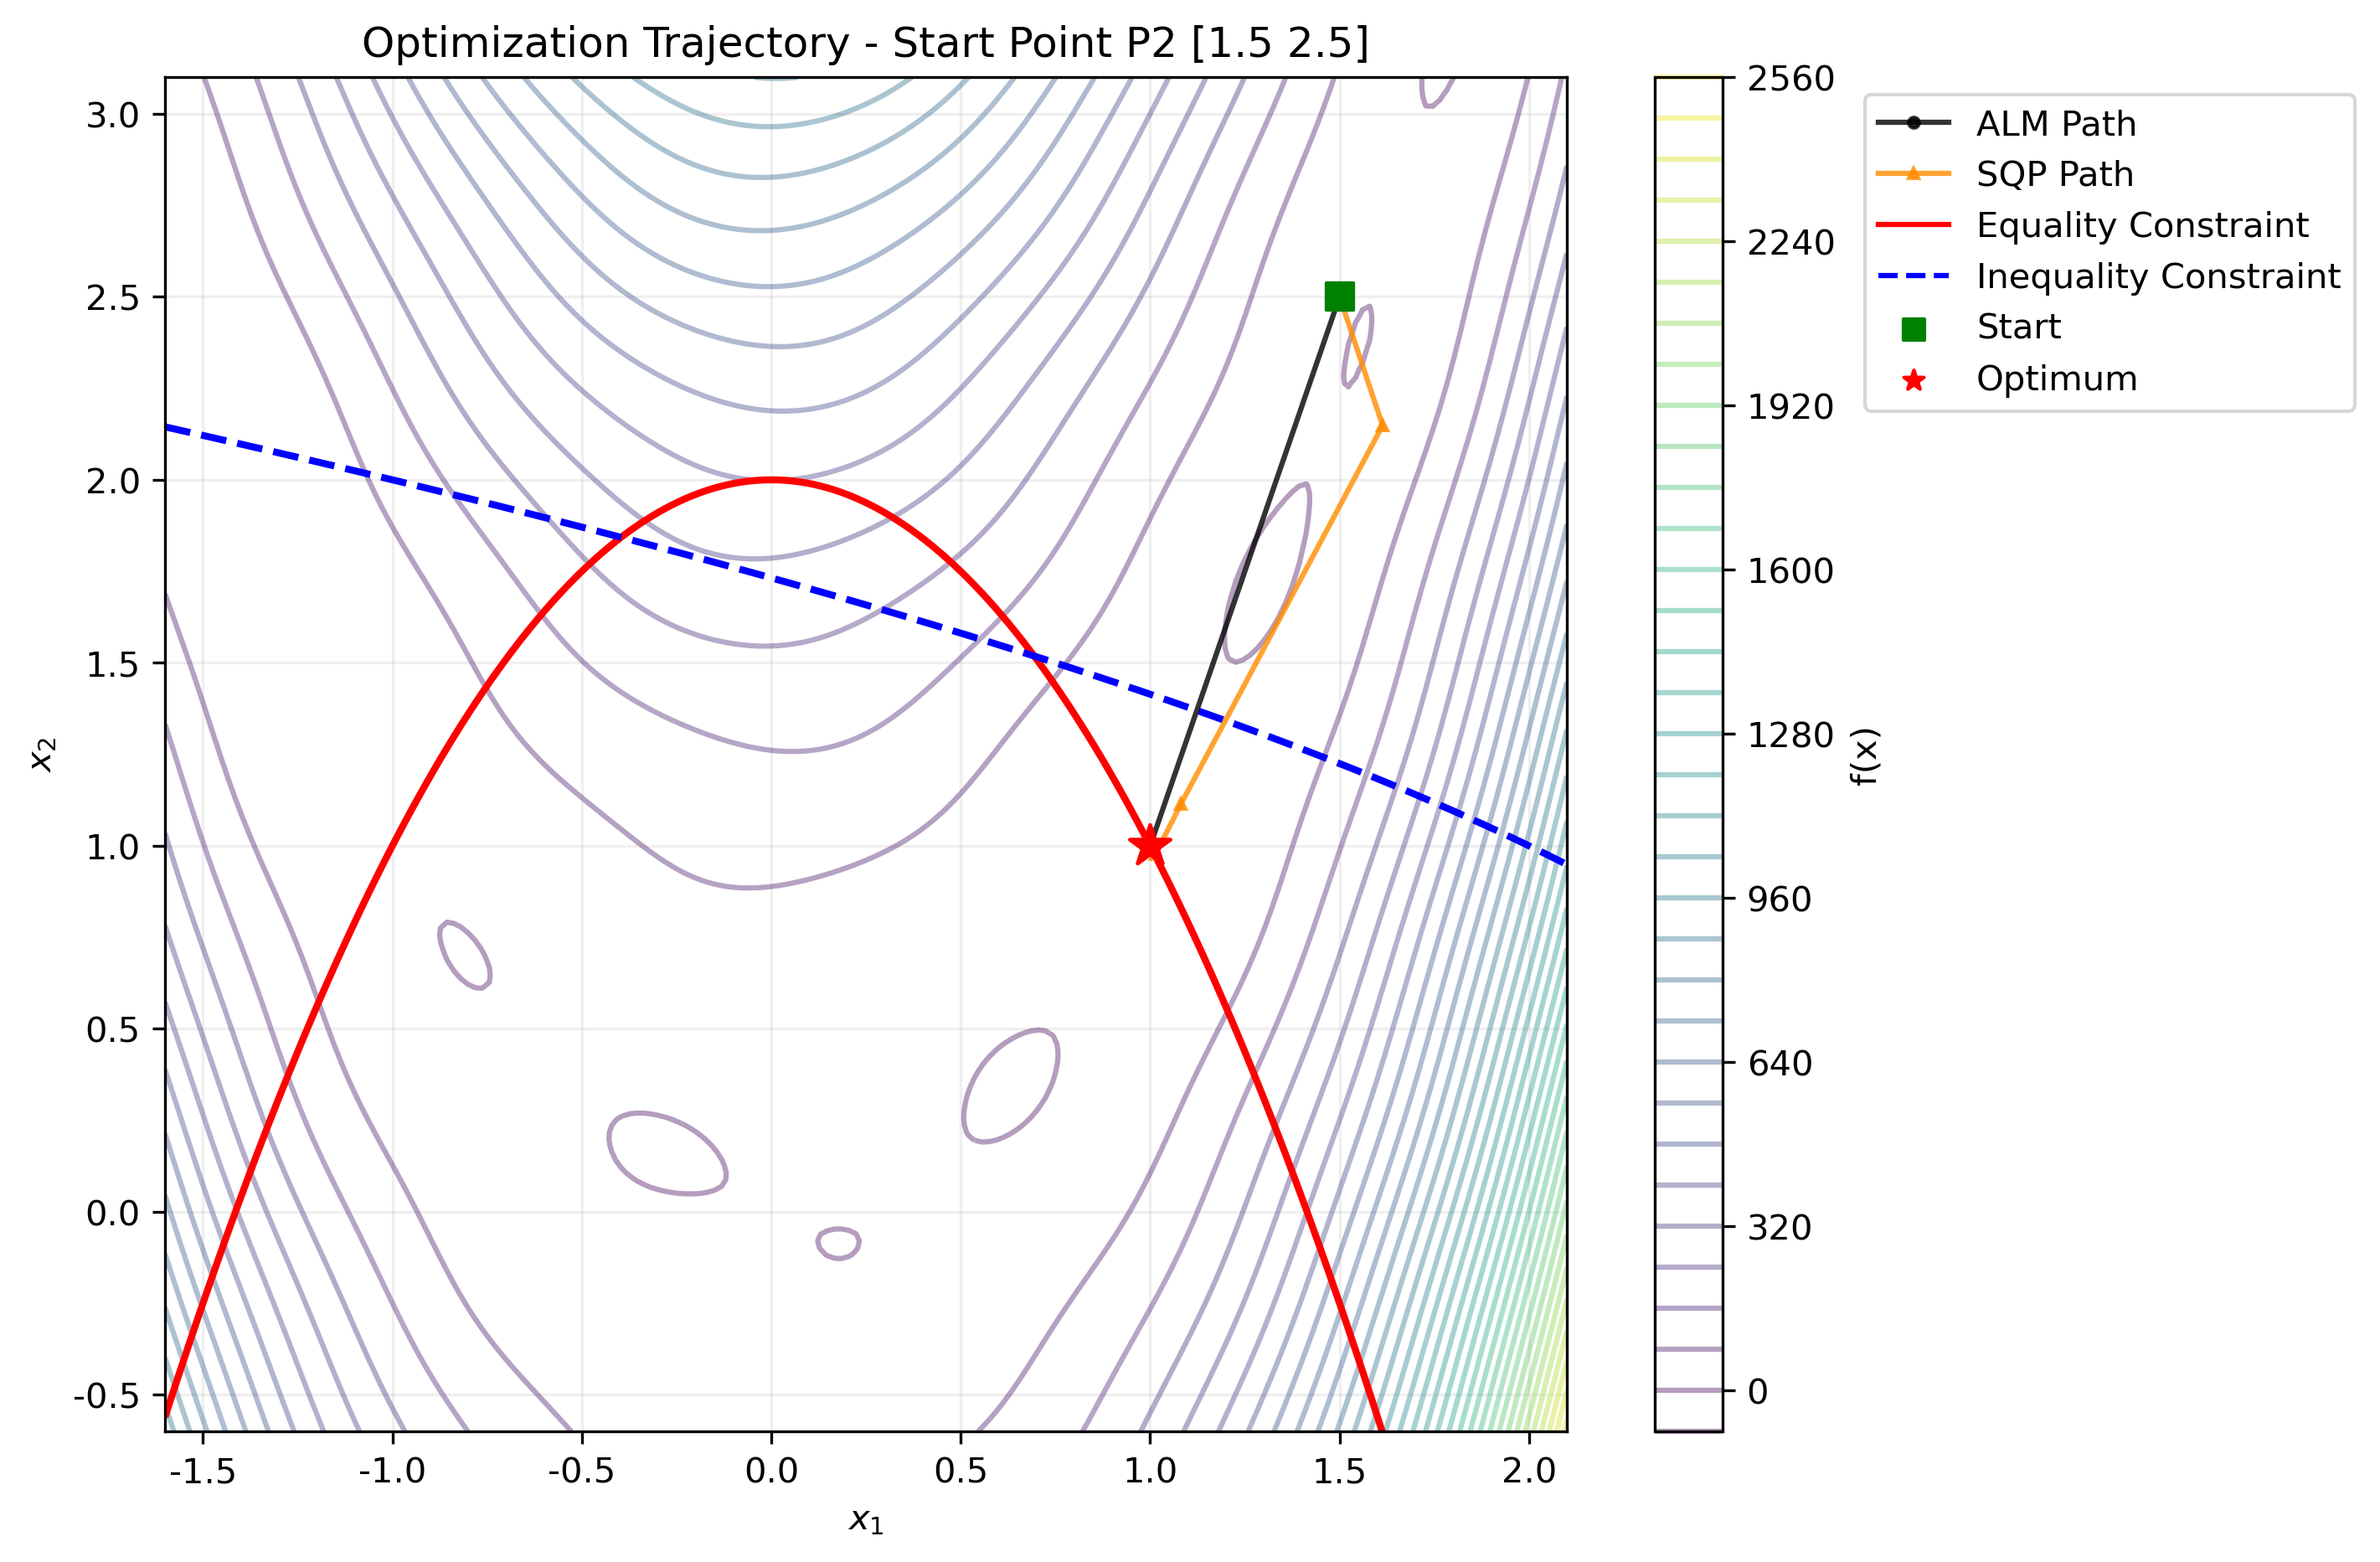
\includegraphics[width=\textwidth]{figures/path_2D_P2.png}
%         \caption{$P_2$: Global Optima}
%     \end{subfigure}
    
%     \vspace{0.3em} % 缩小垂直间距
    
%     % 第二行
%     \begin{subfigure}[b]{0.48\textwidth}
%         \centering
%         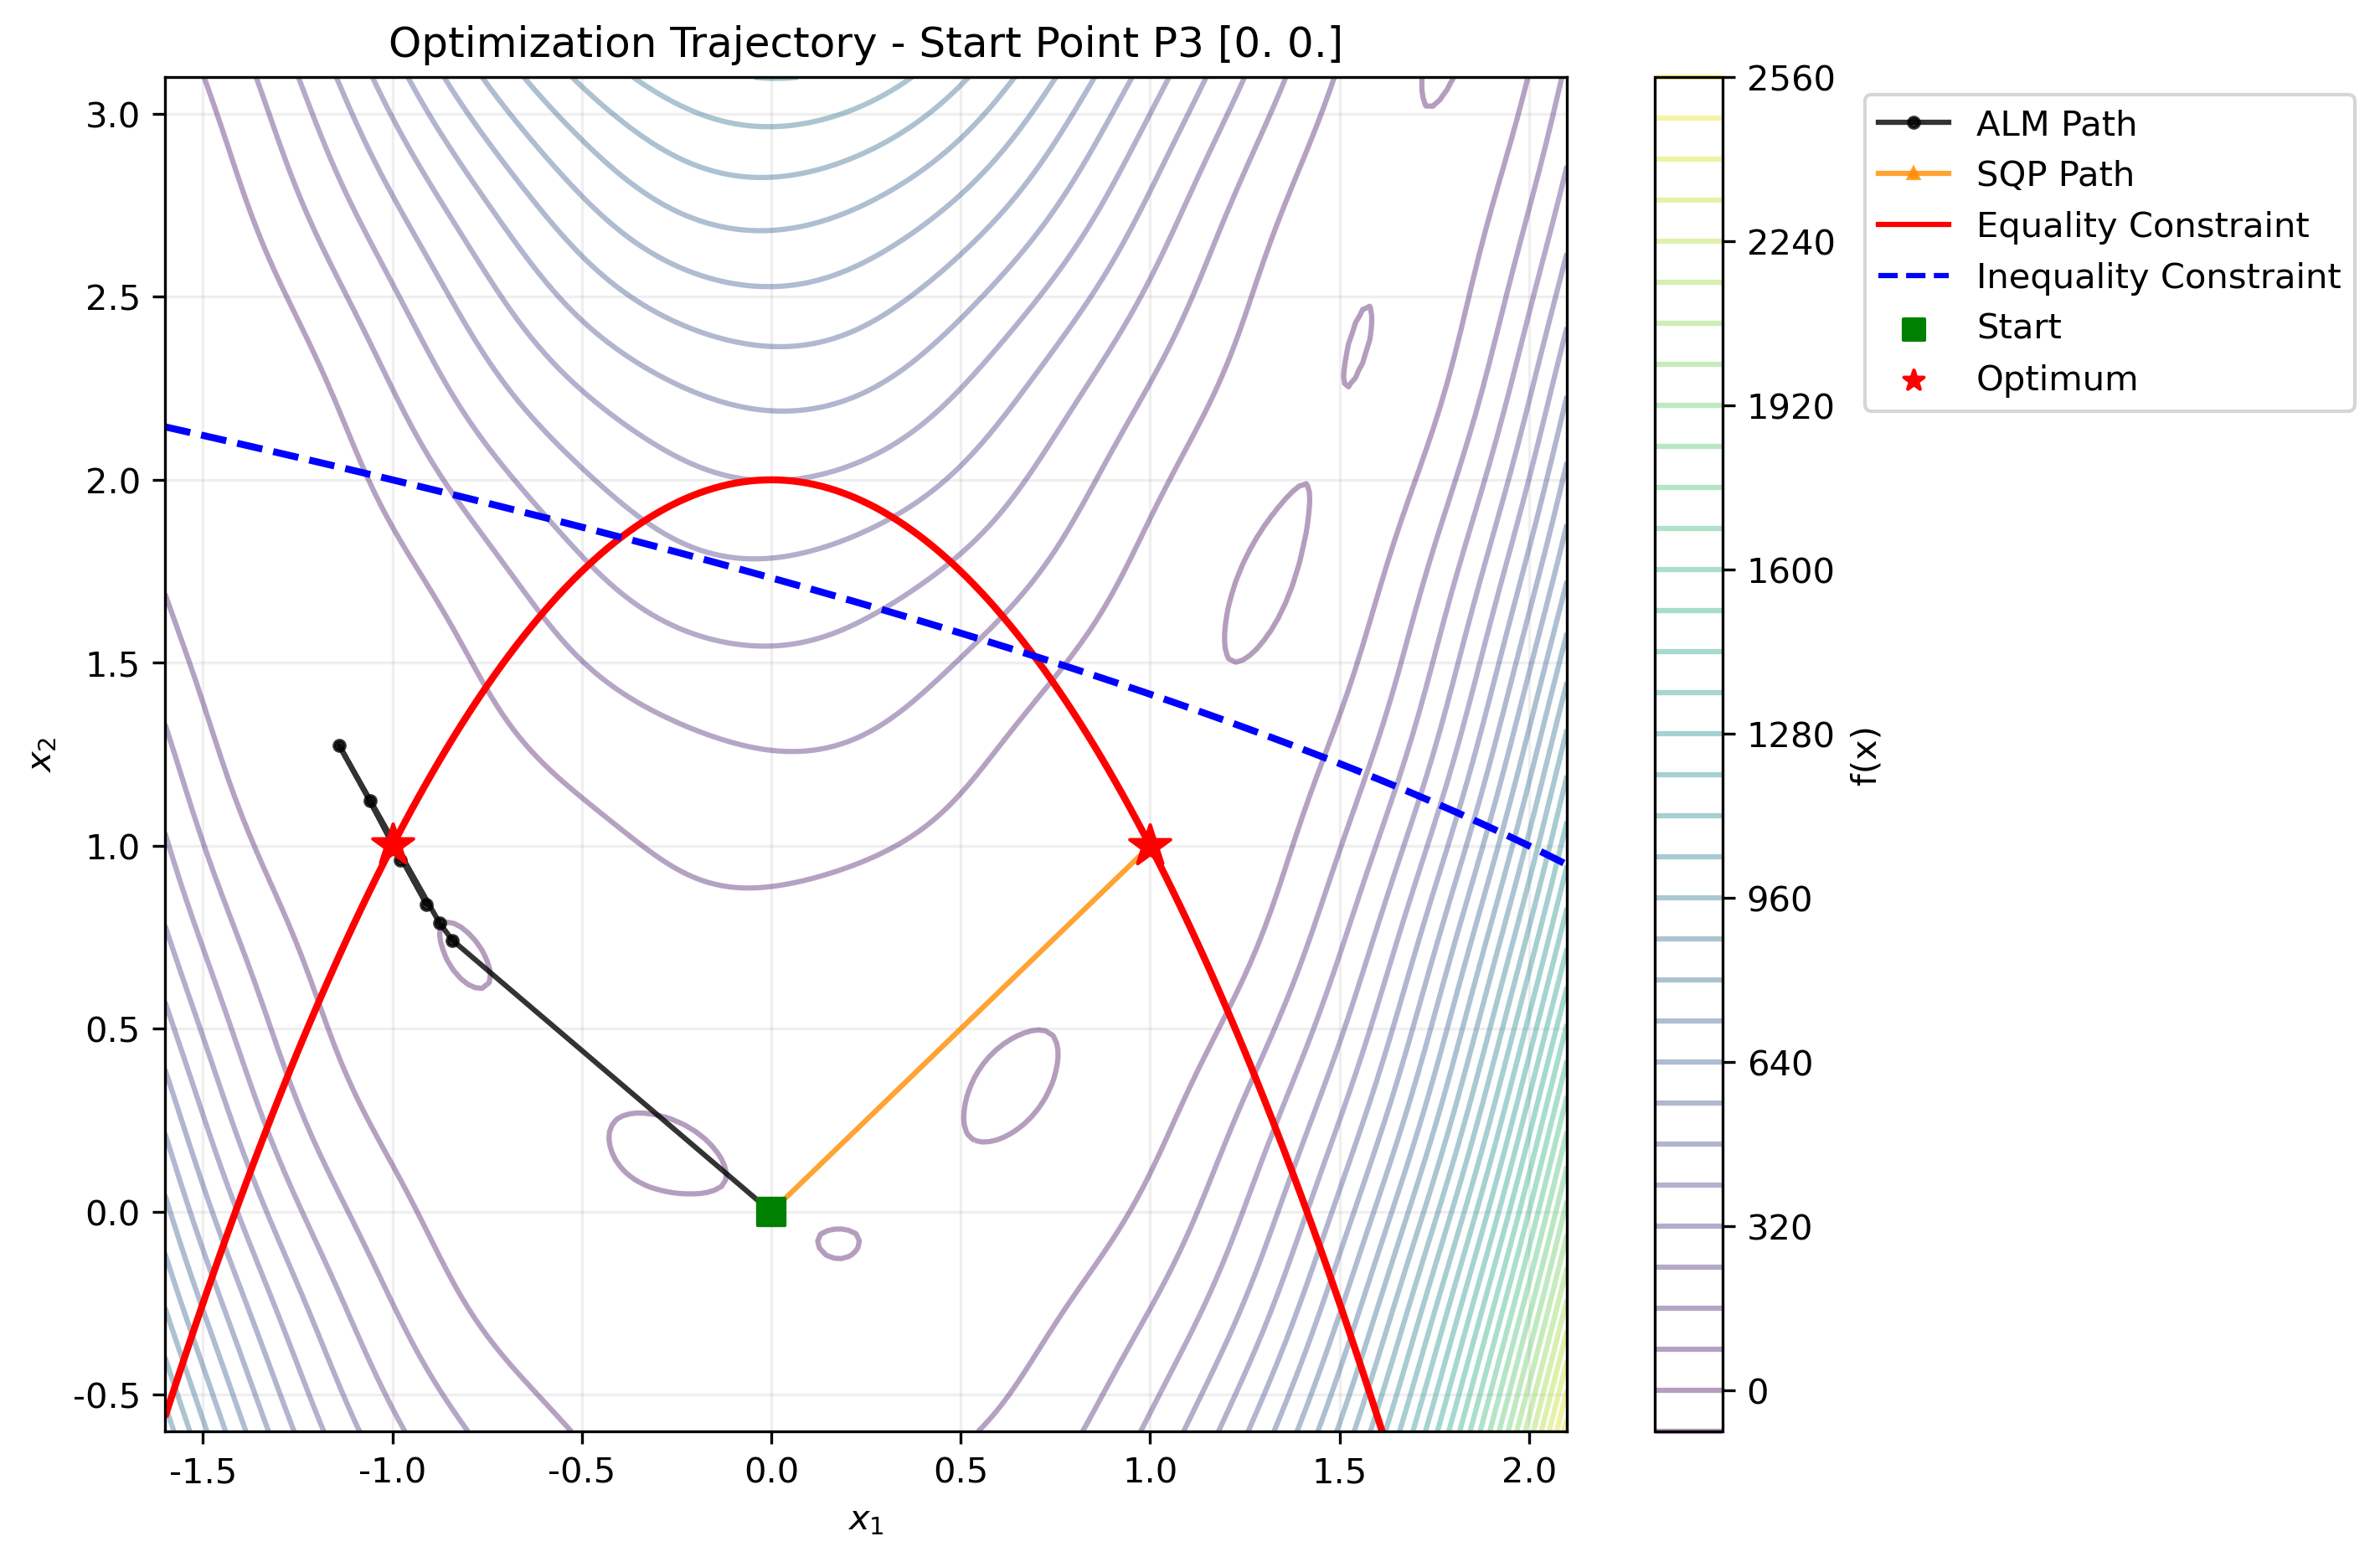
\includegraphics[width=\textwidth]{figures/path_2D_P3.png}
%         \caption{$P_3$: Saddle Point}
%     \end{subfigure}
%     \hfill
%     \begin{subfigure}[b]{0.48\textwidth}
%         \centering
%         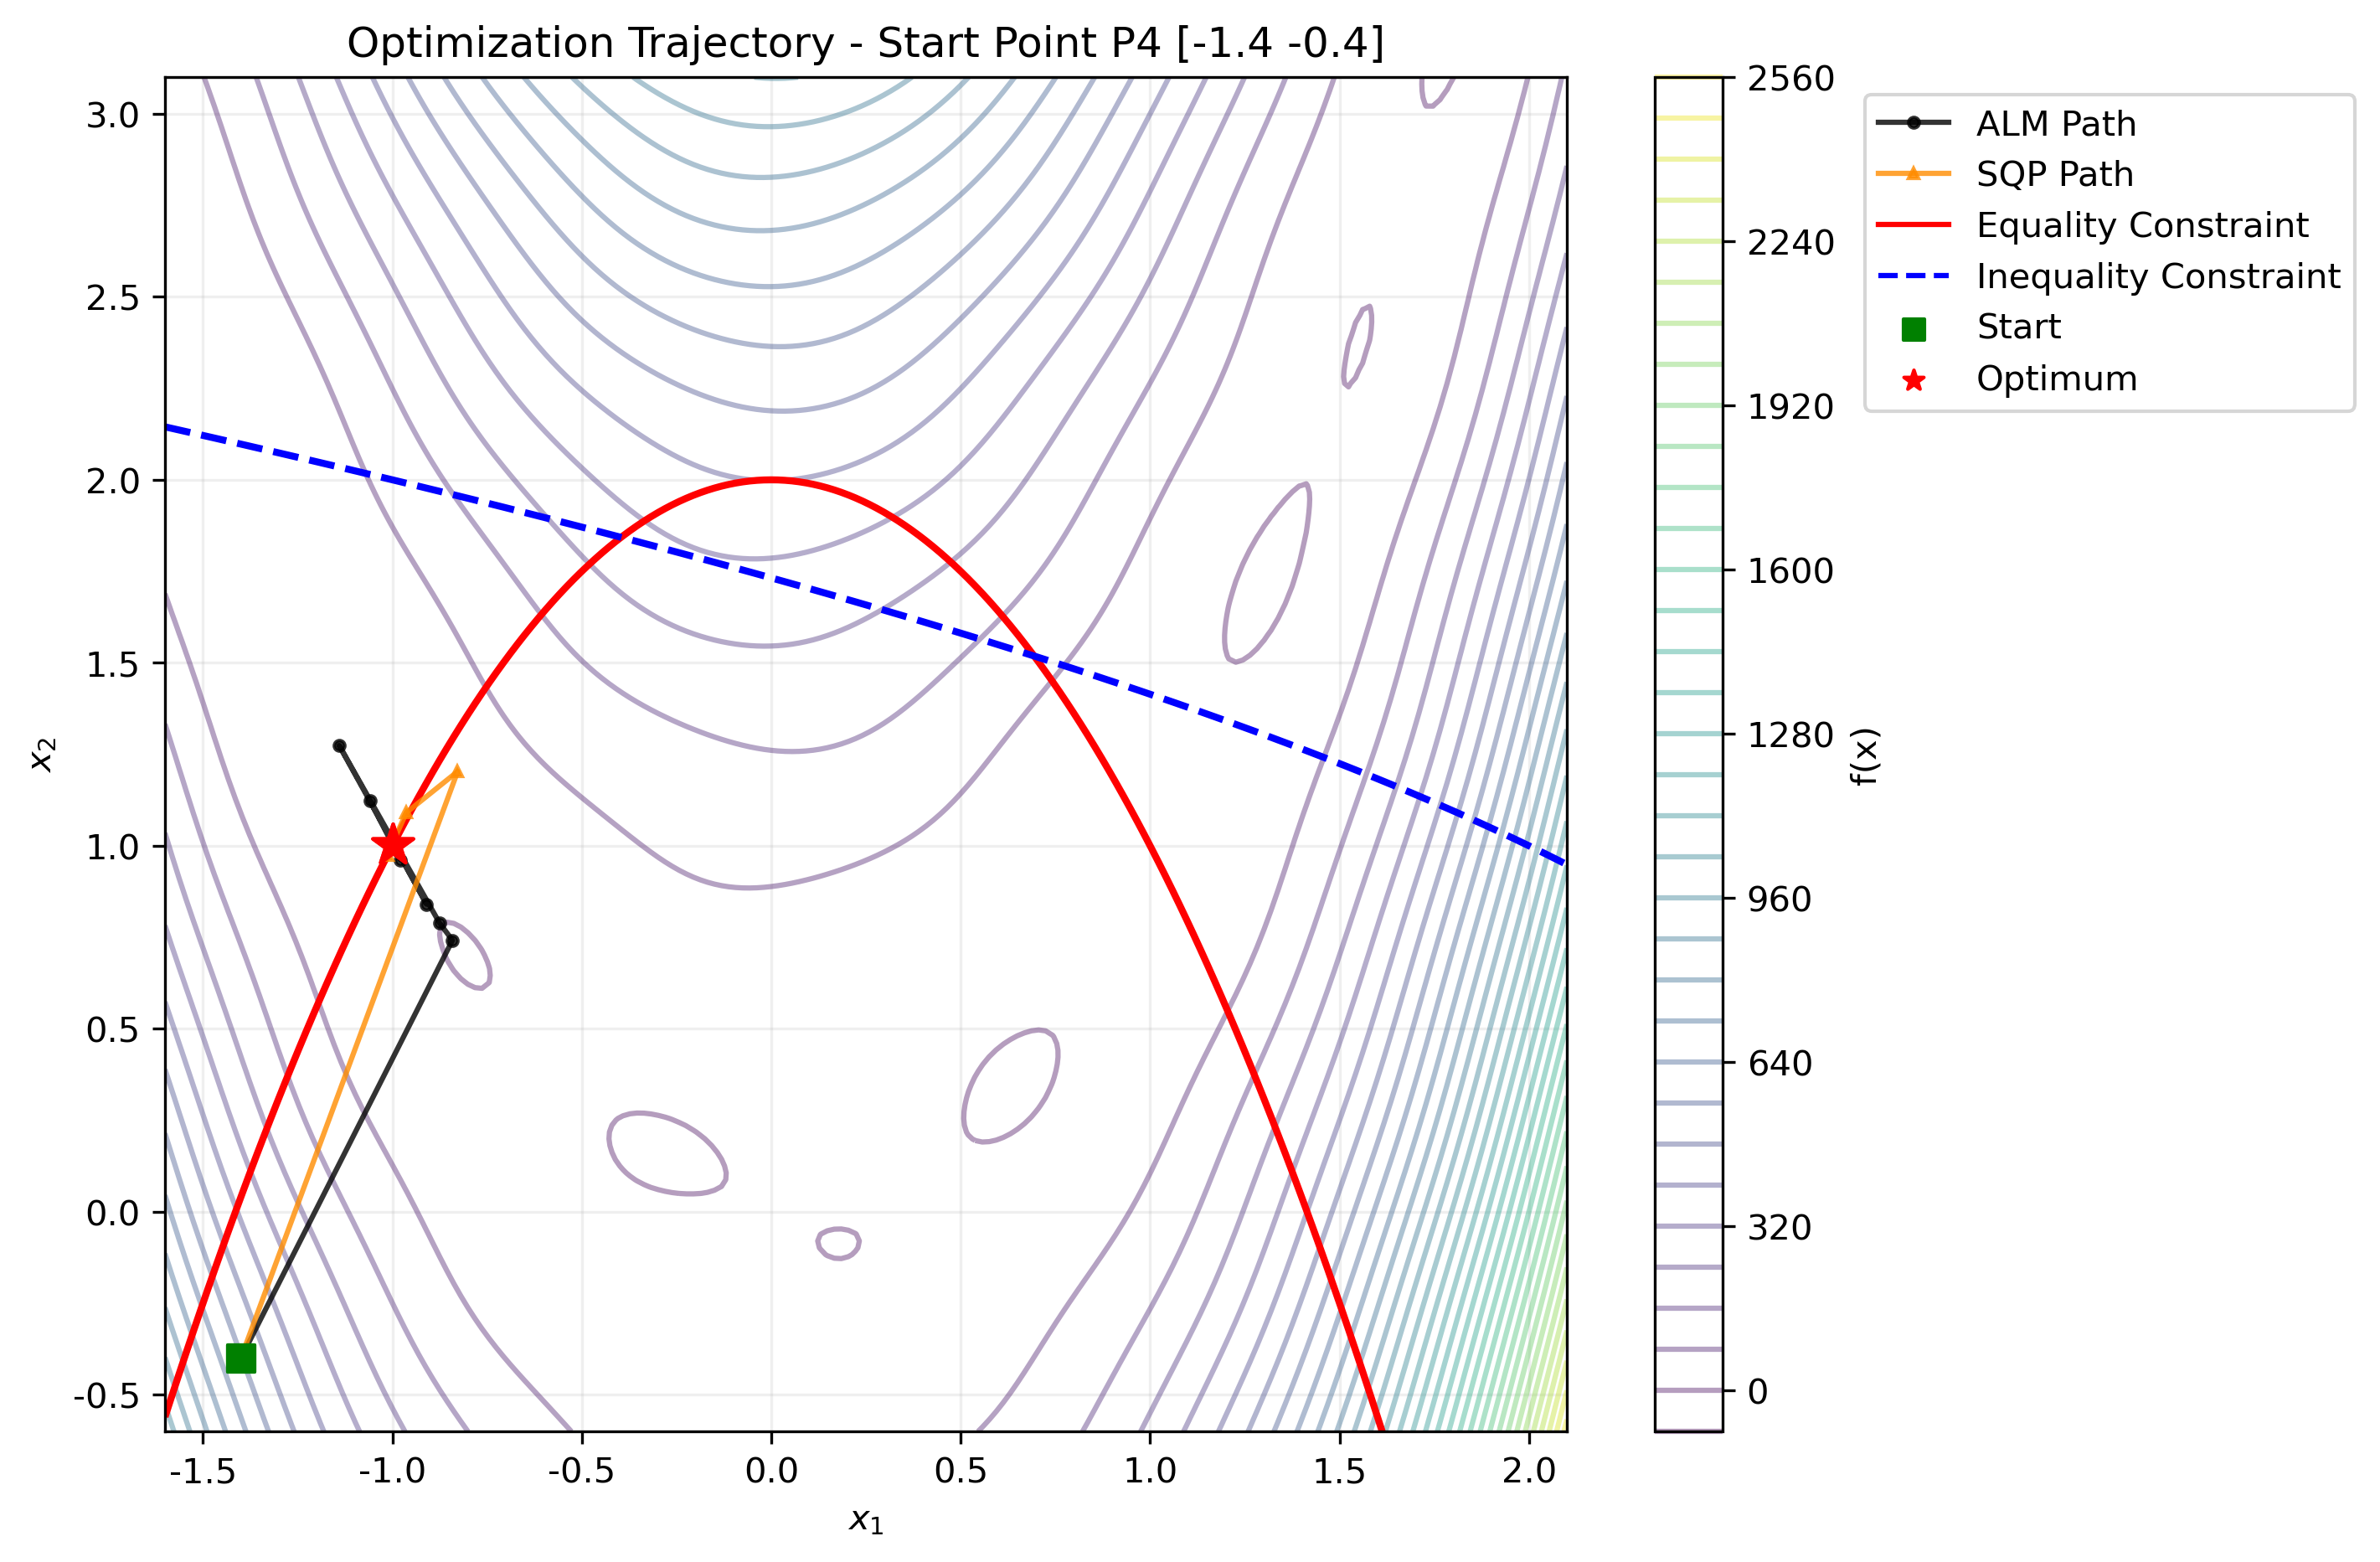
\includegraphics[width=\textwidth]{figures/path_2D_P4.png}
%         \caption{$P_4$: Boundary Start}
%     \end{subfigure}
    
%     \vspace{0.3em} % 缩小垂直间距

    
%     % 第三行
%     \begin{subfigure}[b]{0.48\textwidth}
%         \centering
%         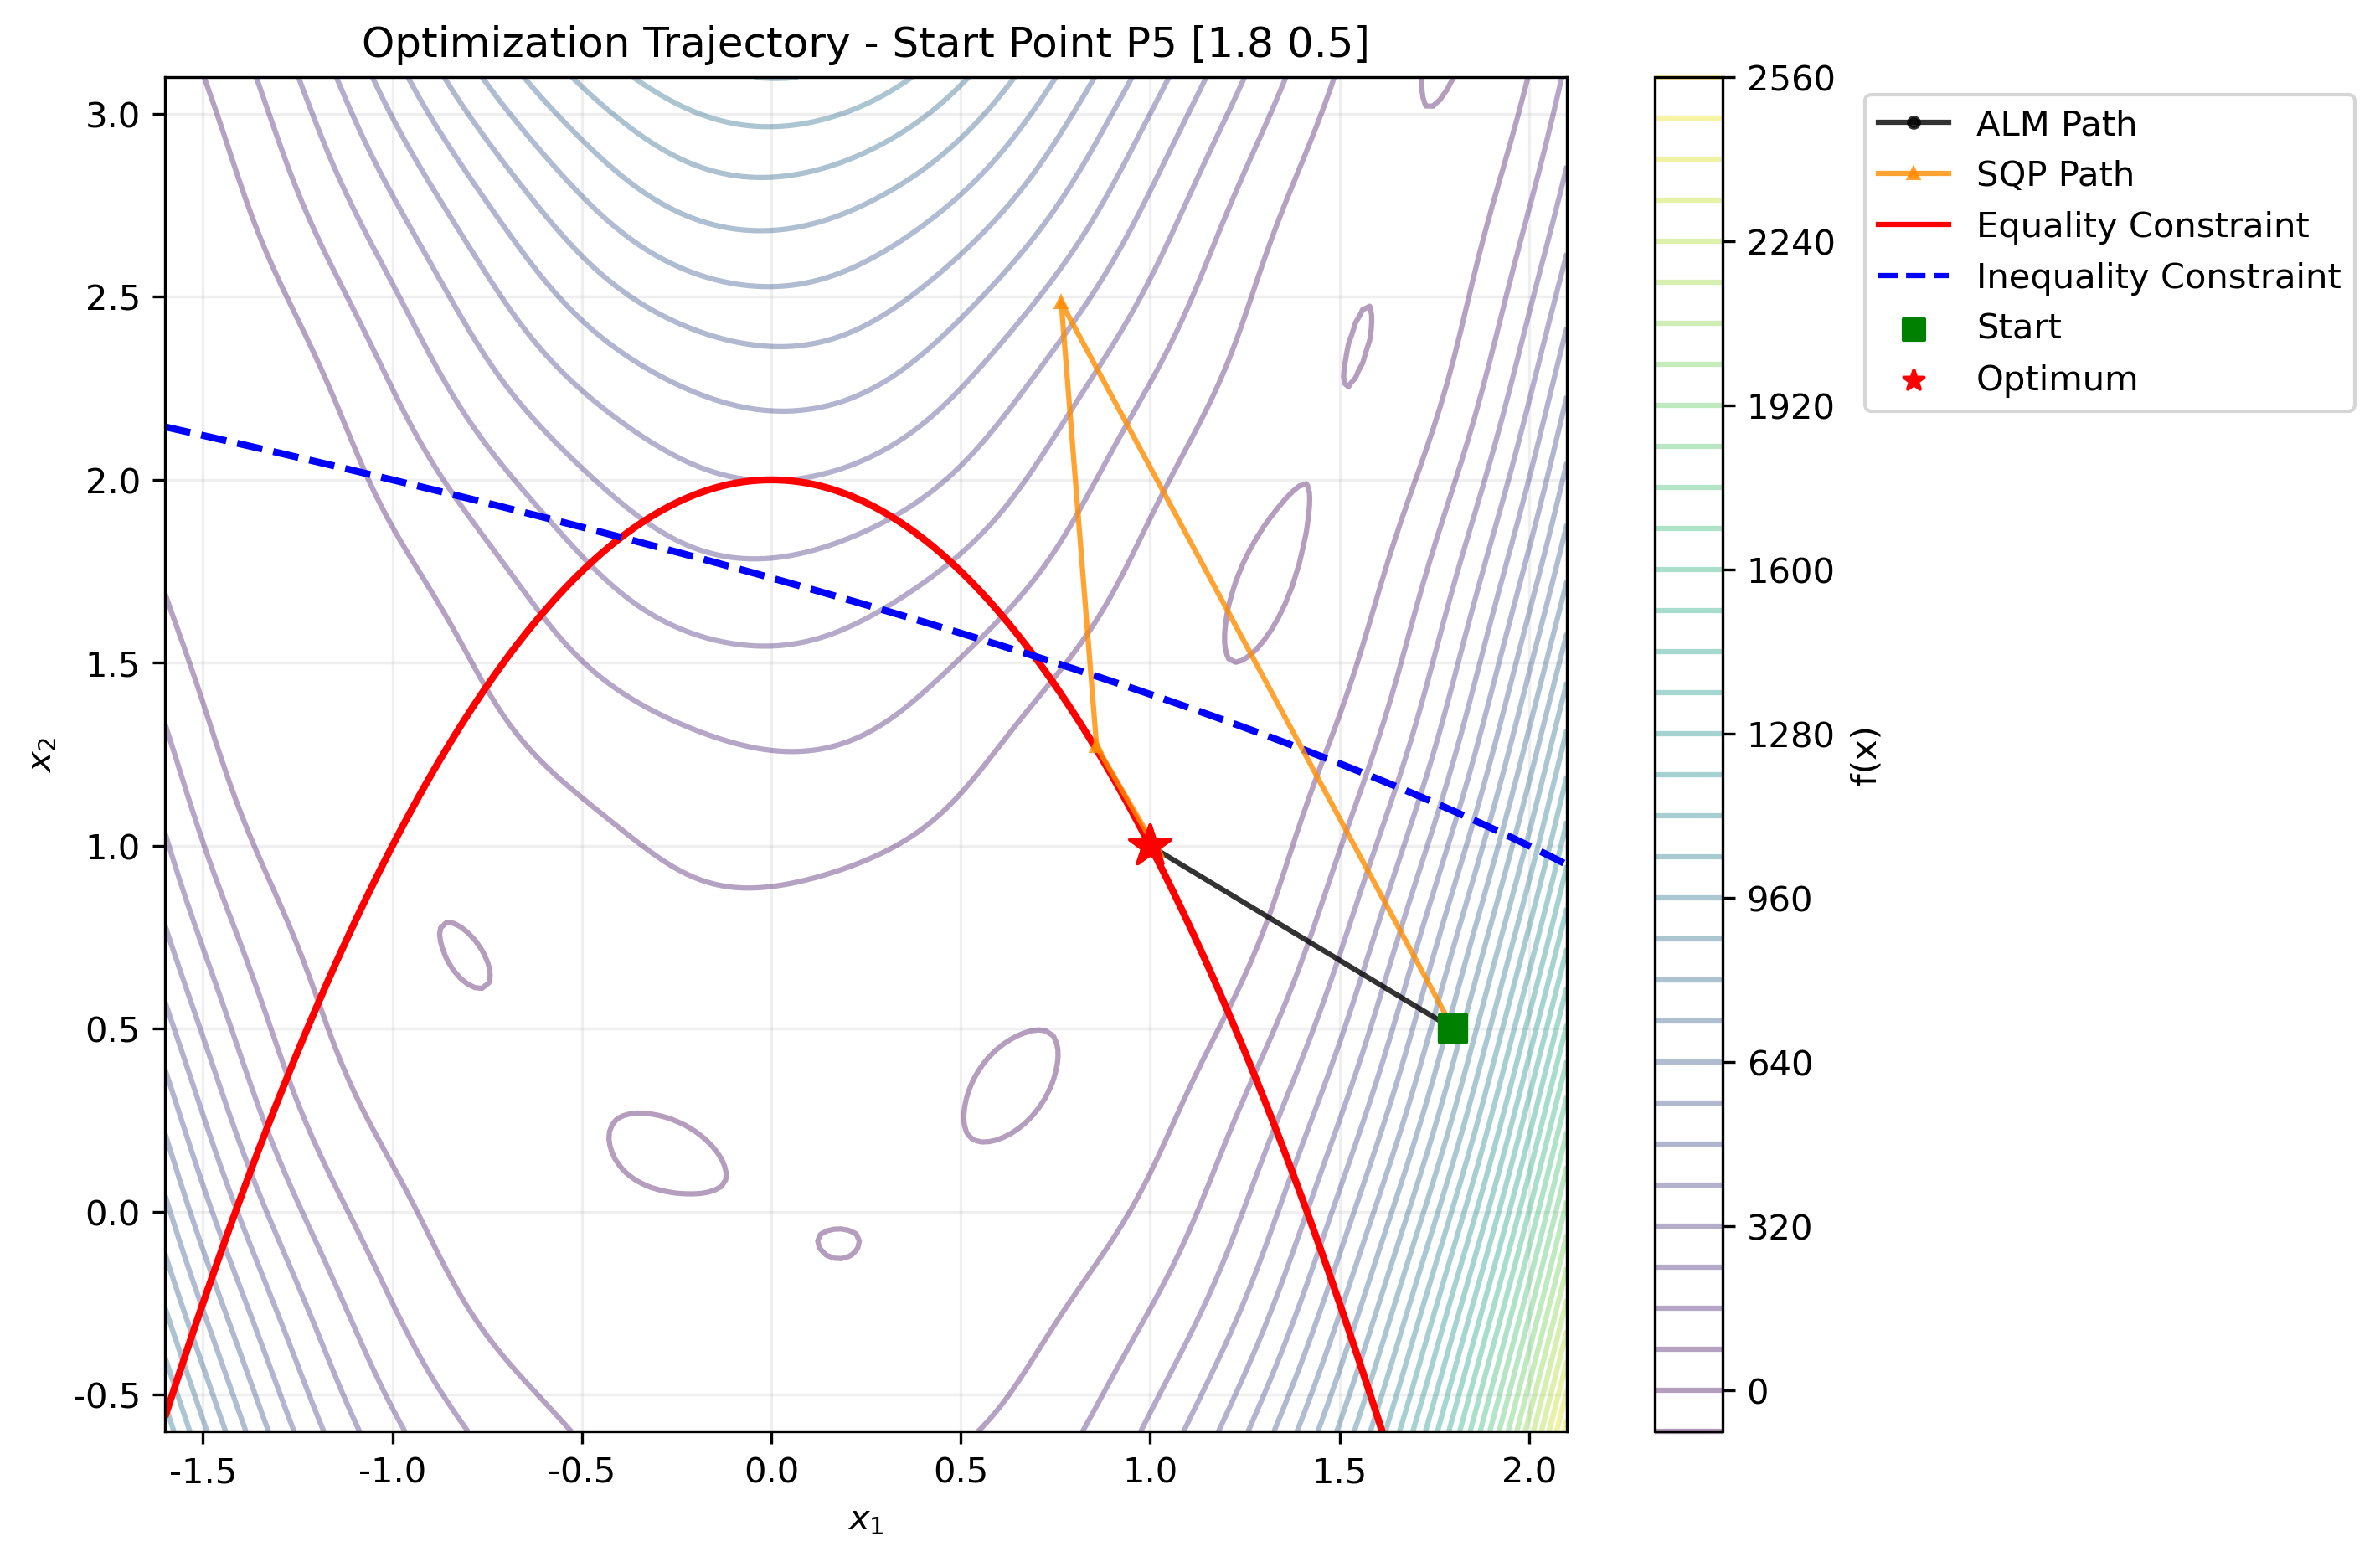
\includegraphics[width=\textwidth]{figures/path_2D_P5.png}
%         \caption{$P_5$: Right Boundary}
%     \end{subfigure}
%     \hfill
%     \begin{subfigure}[b]{0.48\textwidth}
%         \centering
%         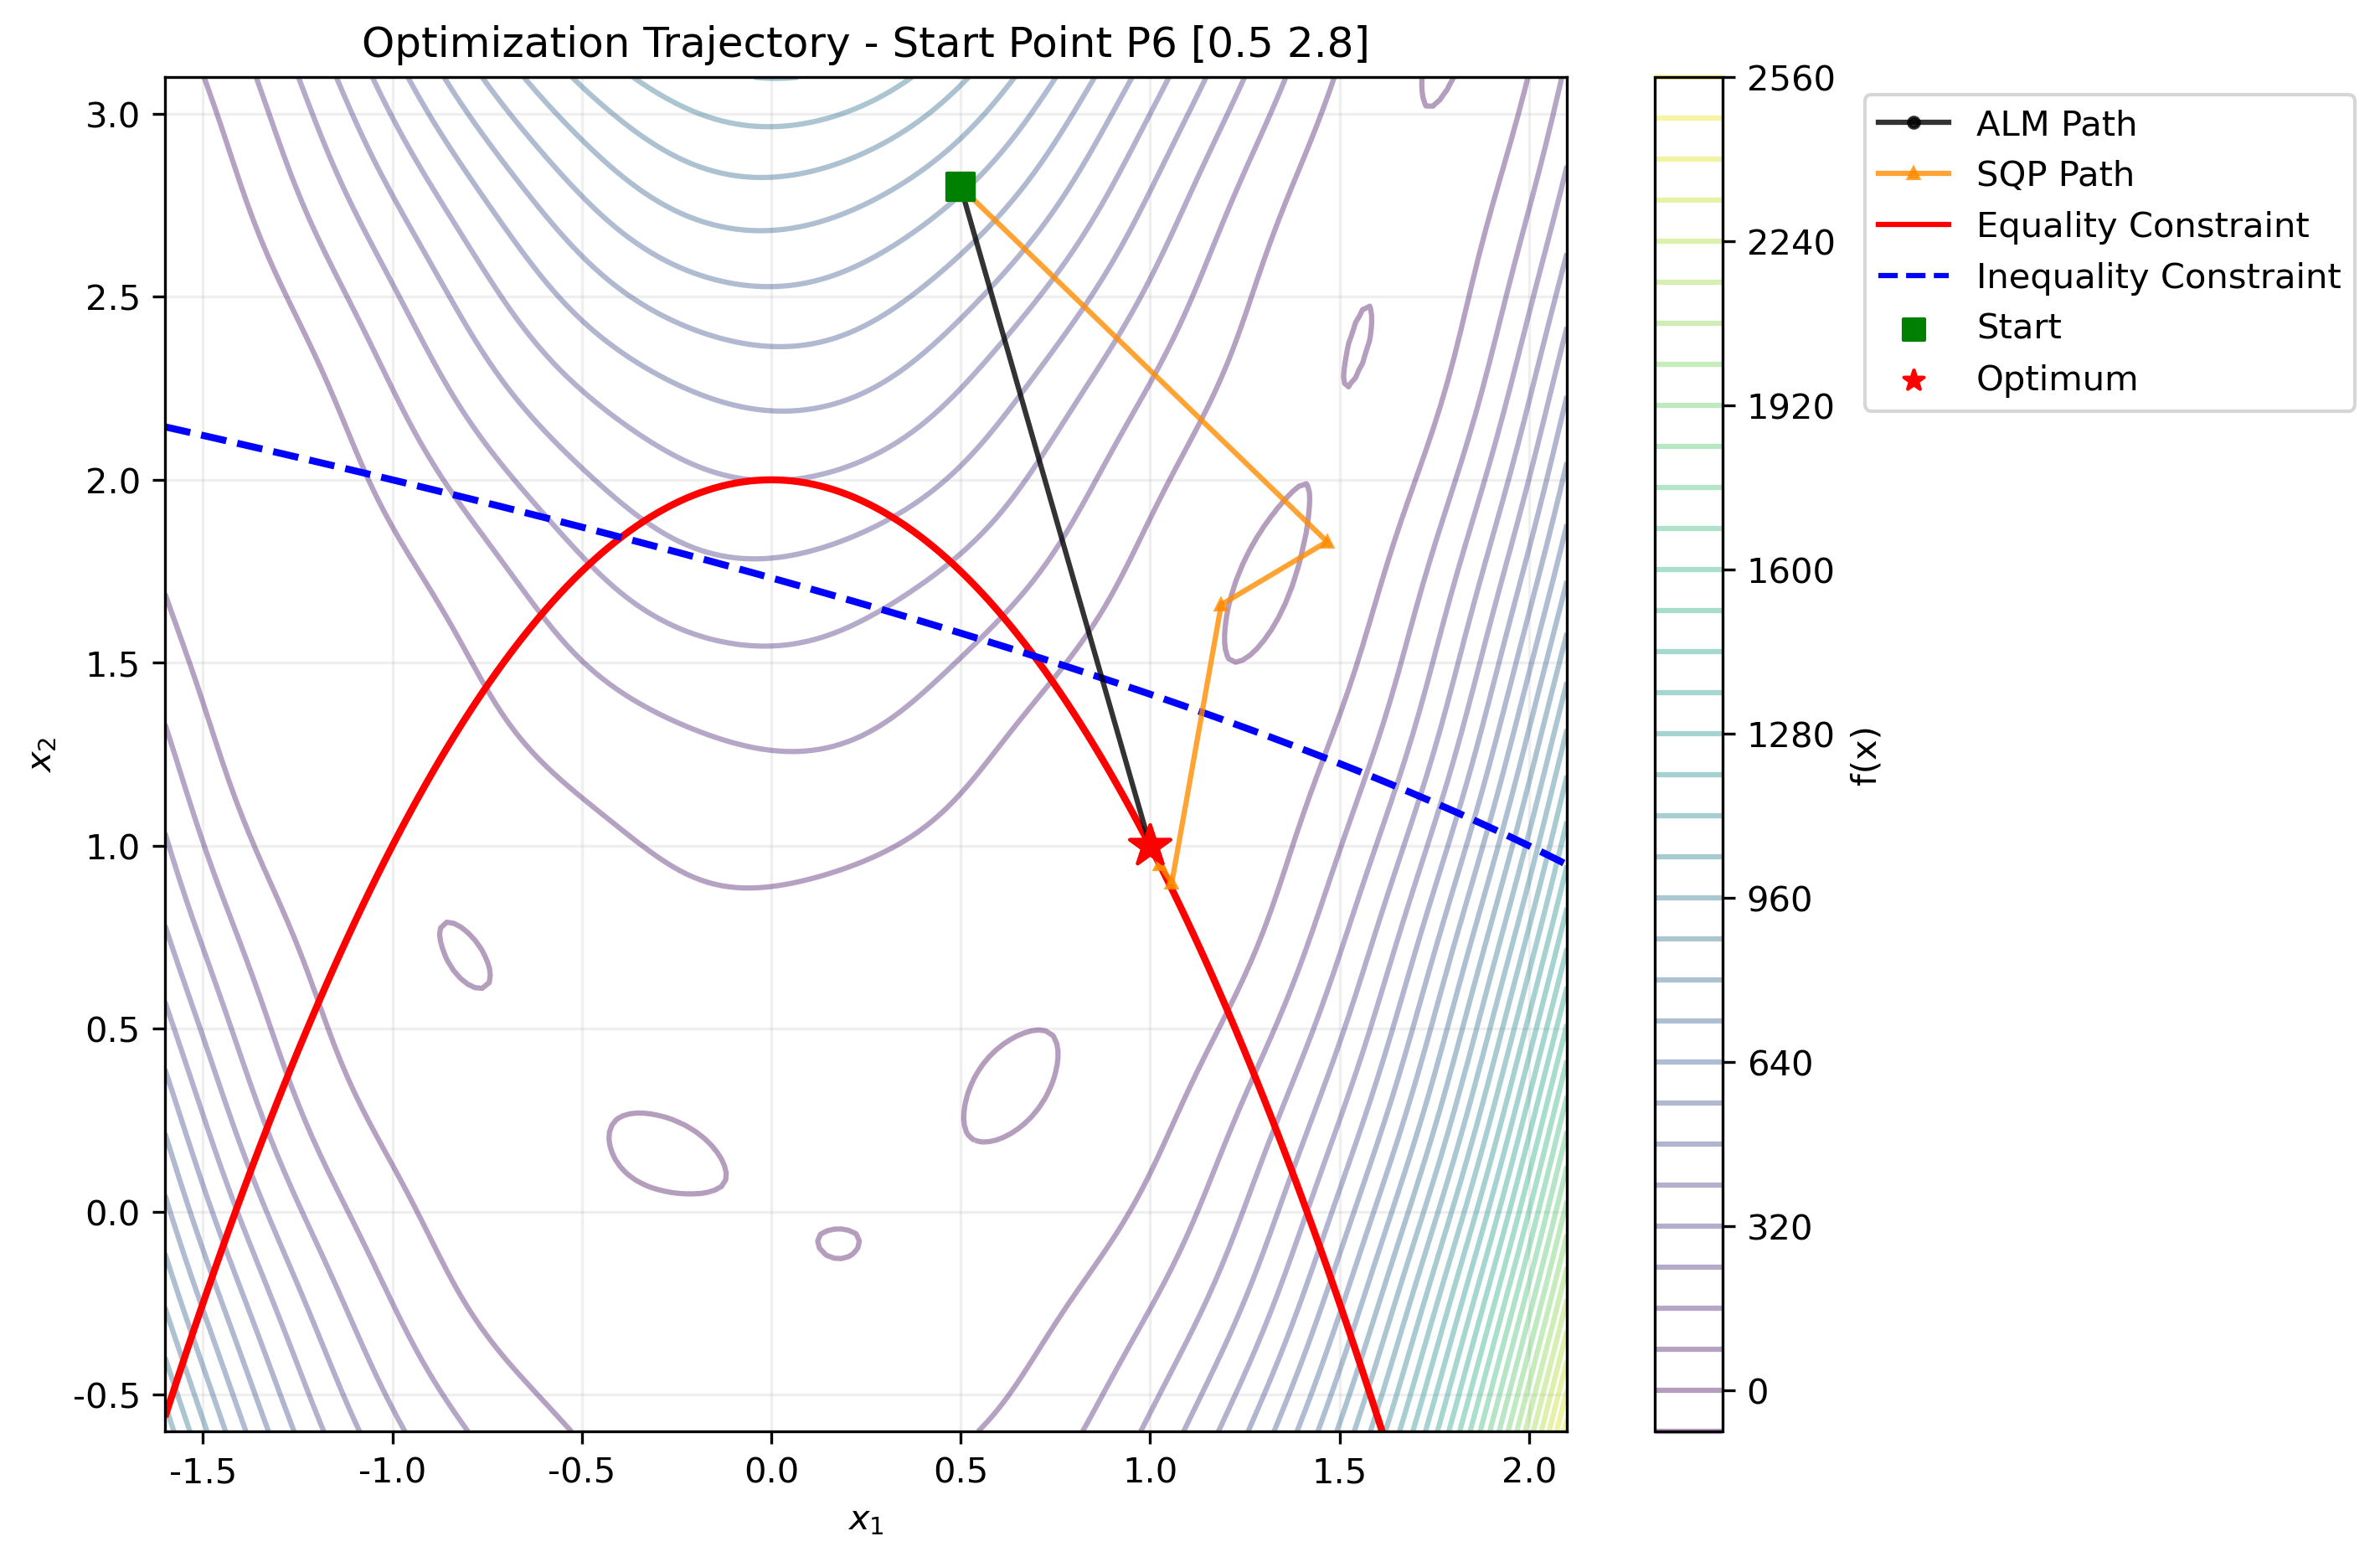
\includegraphics[width=\textwidth]{figures/path_2D_P6.png}
%         \caption{$P_6$: High Infeasible}
%     \end{subfigure}
    
%     \vspace{0.3em} % 缩小垂直间距

    
%     % 第四行
%     \begin{subfigure}[b]{0.48\textwidth}
%         \centering
%         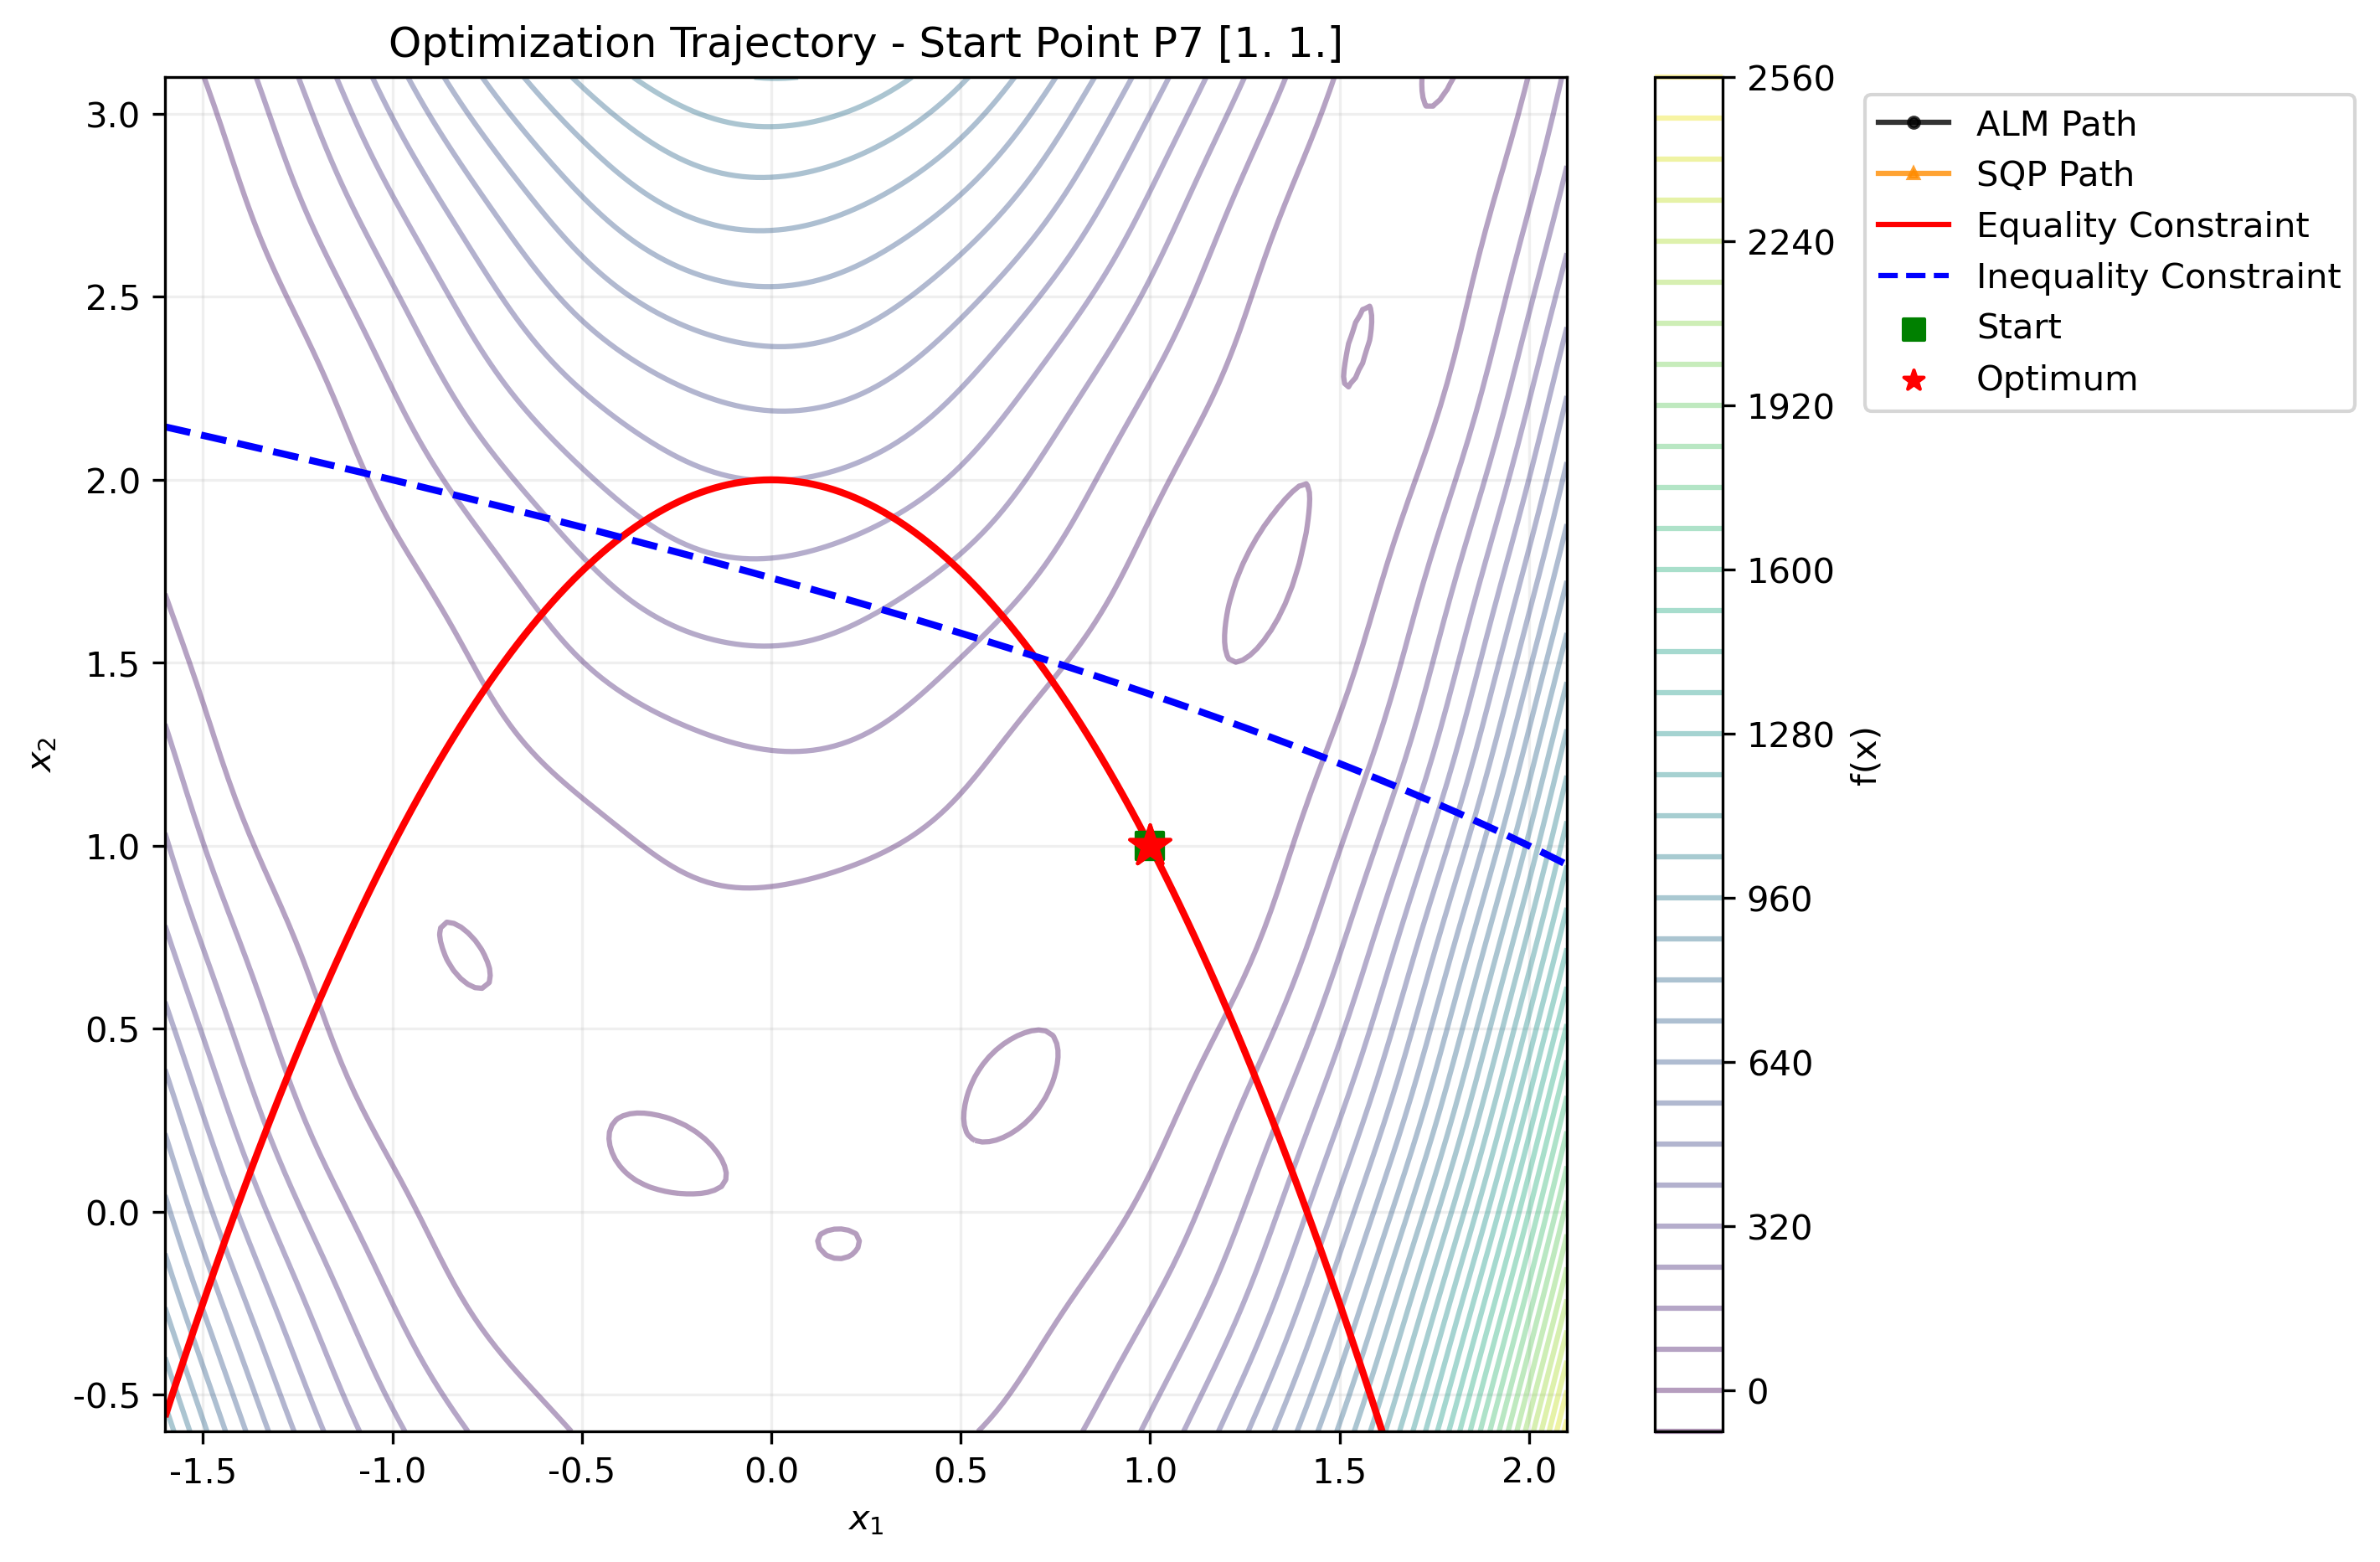
\includegraphics[width=\textwidth]{figures/path_2D_P7.png}
%         \caption{$P_7$: Near Optima}
%     \end{subfigure}
%     \hfill
%     \begin{subfigure}[b]{0.48\textwidth}
%         \centering
%         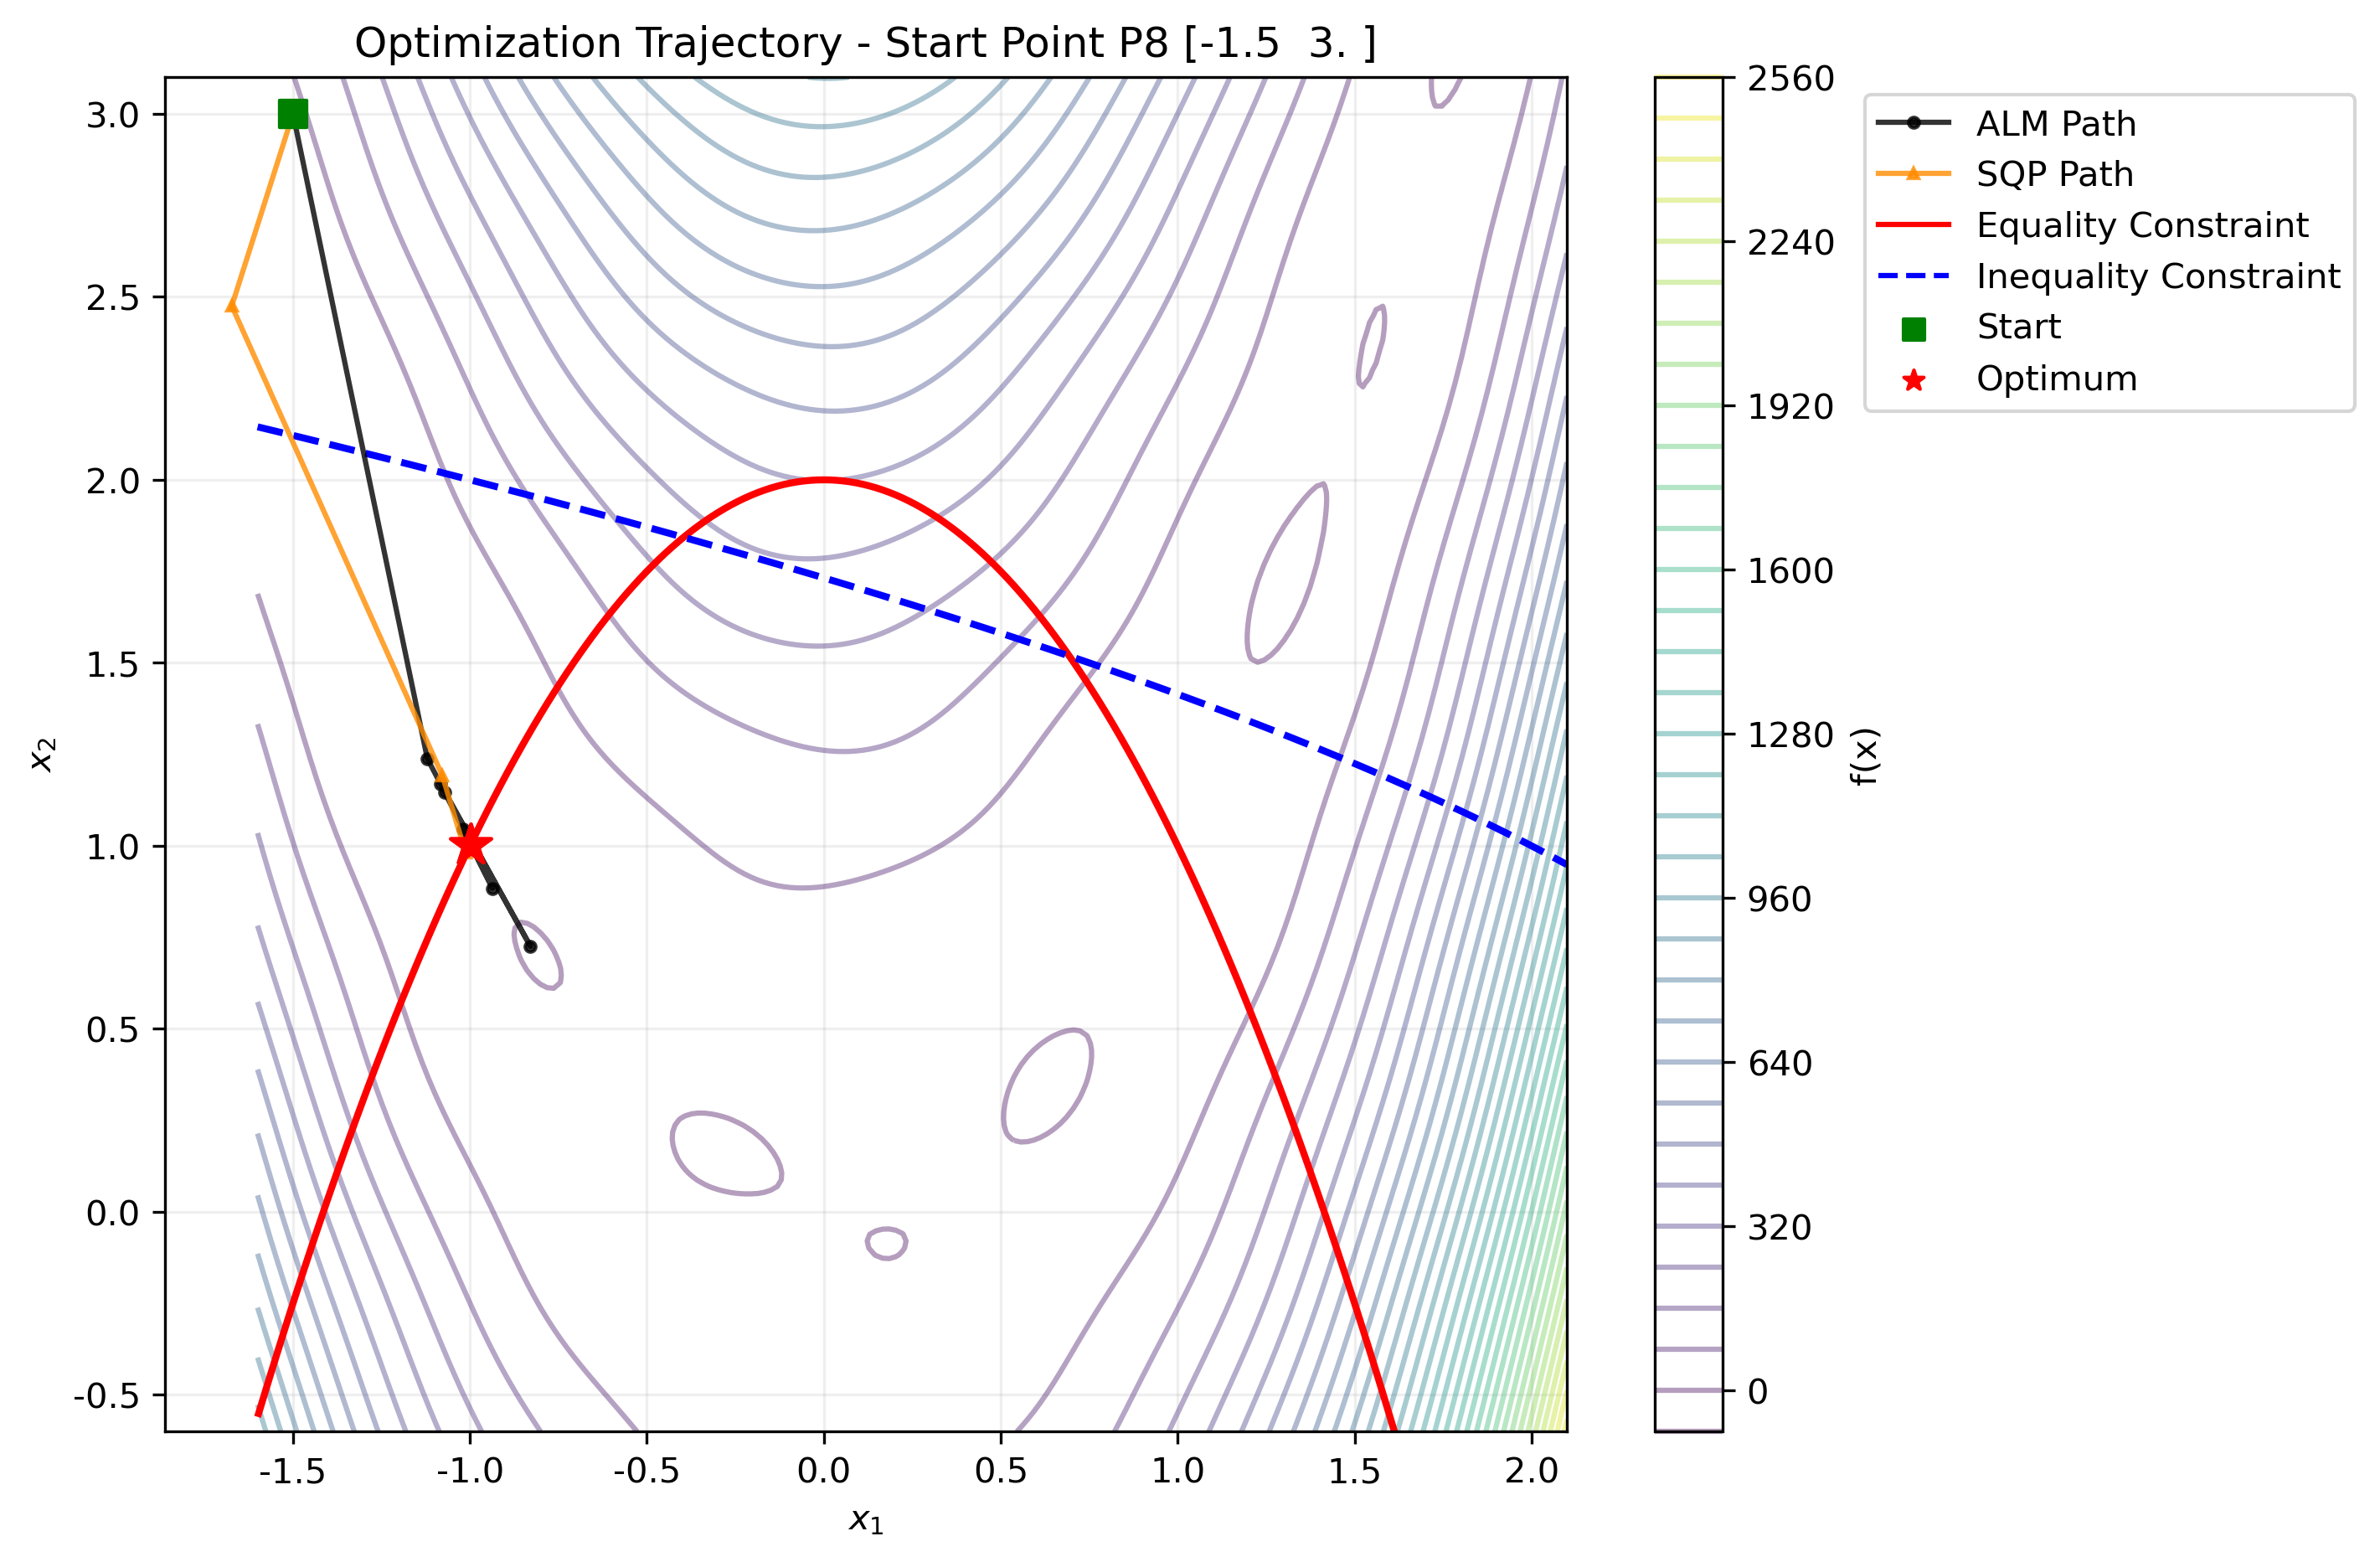
\includegraphics[width=\textwidth]{figures/path_2D_P8.png}
%         \caption{$P_8$: Corner Case}
%     \end{subfigure}
    
%     \vspace{0.3em} % 缩小垂直间距

    
%     % 第五行
%     \begin{subfigure}[b]{0.48\textwidth}
%         \centering
%         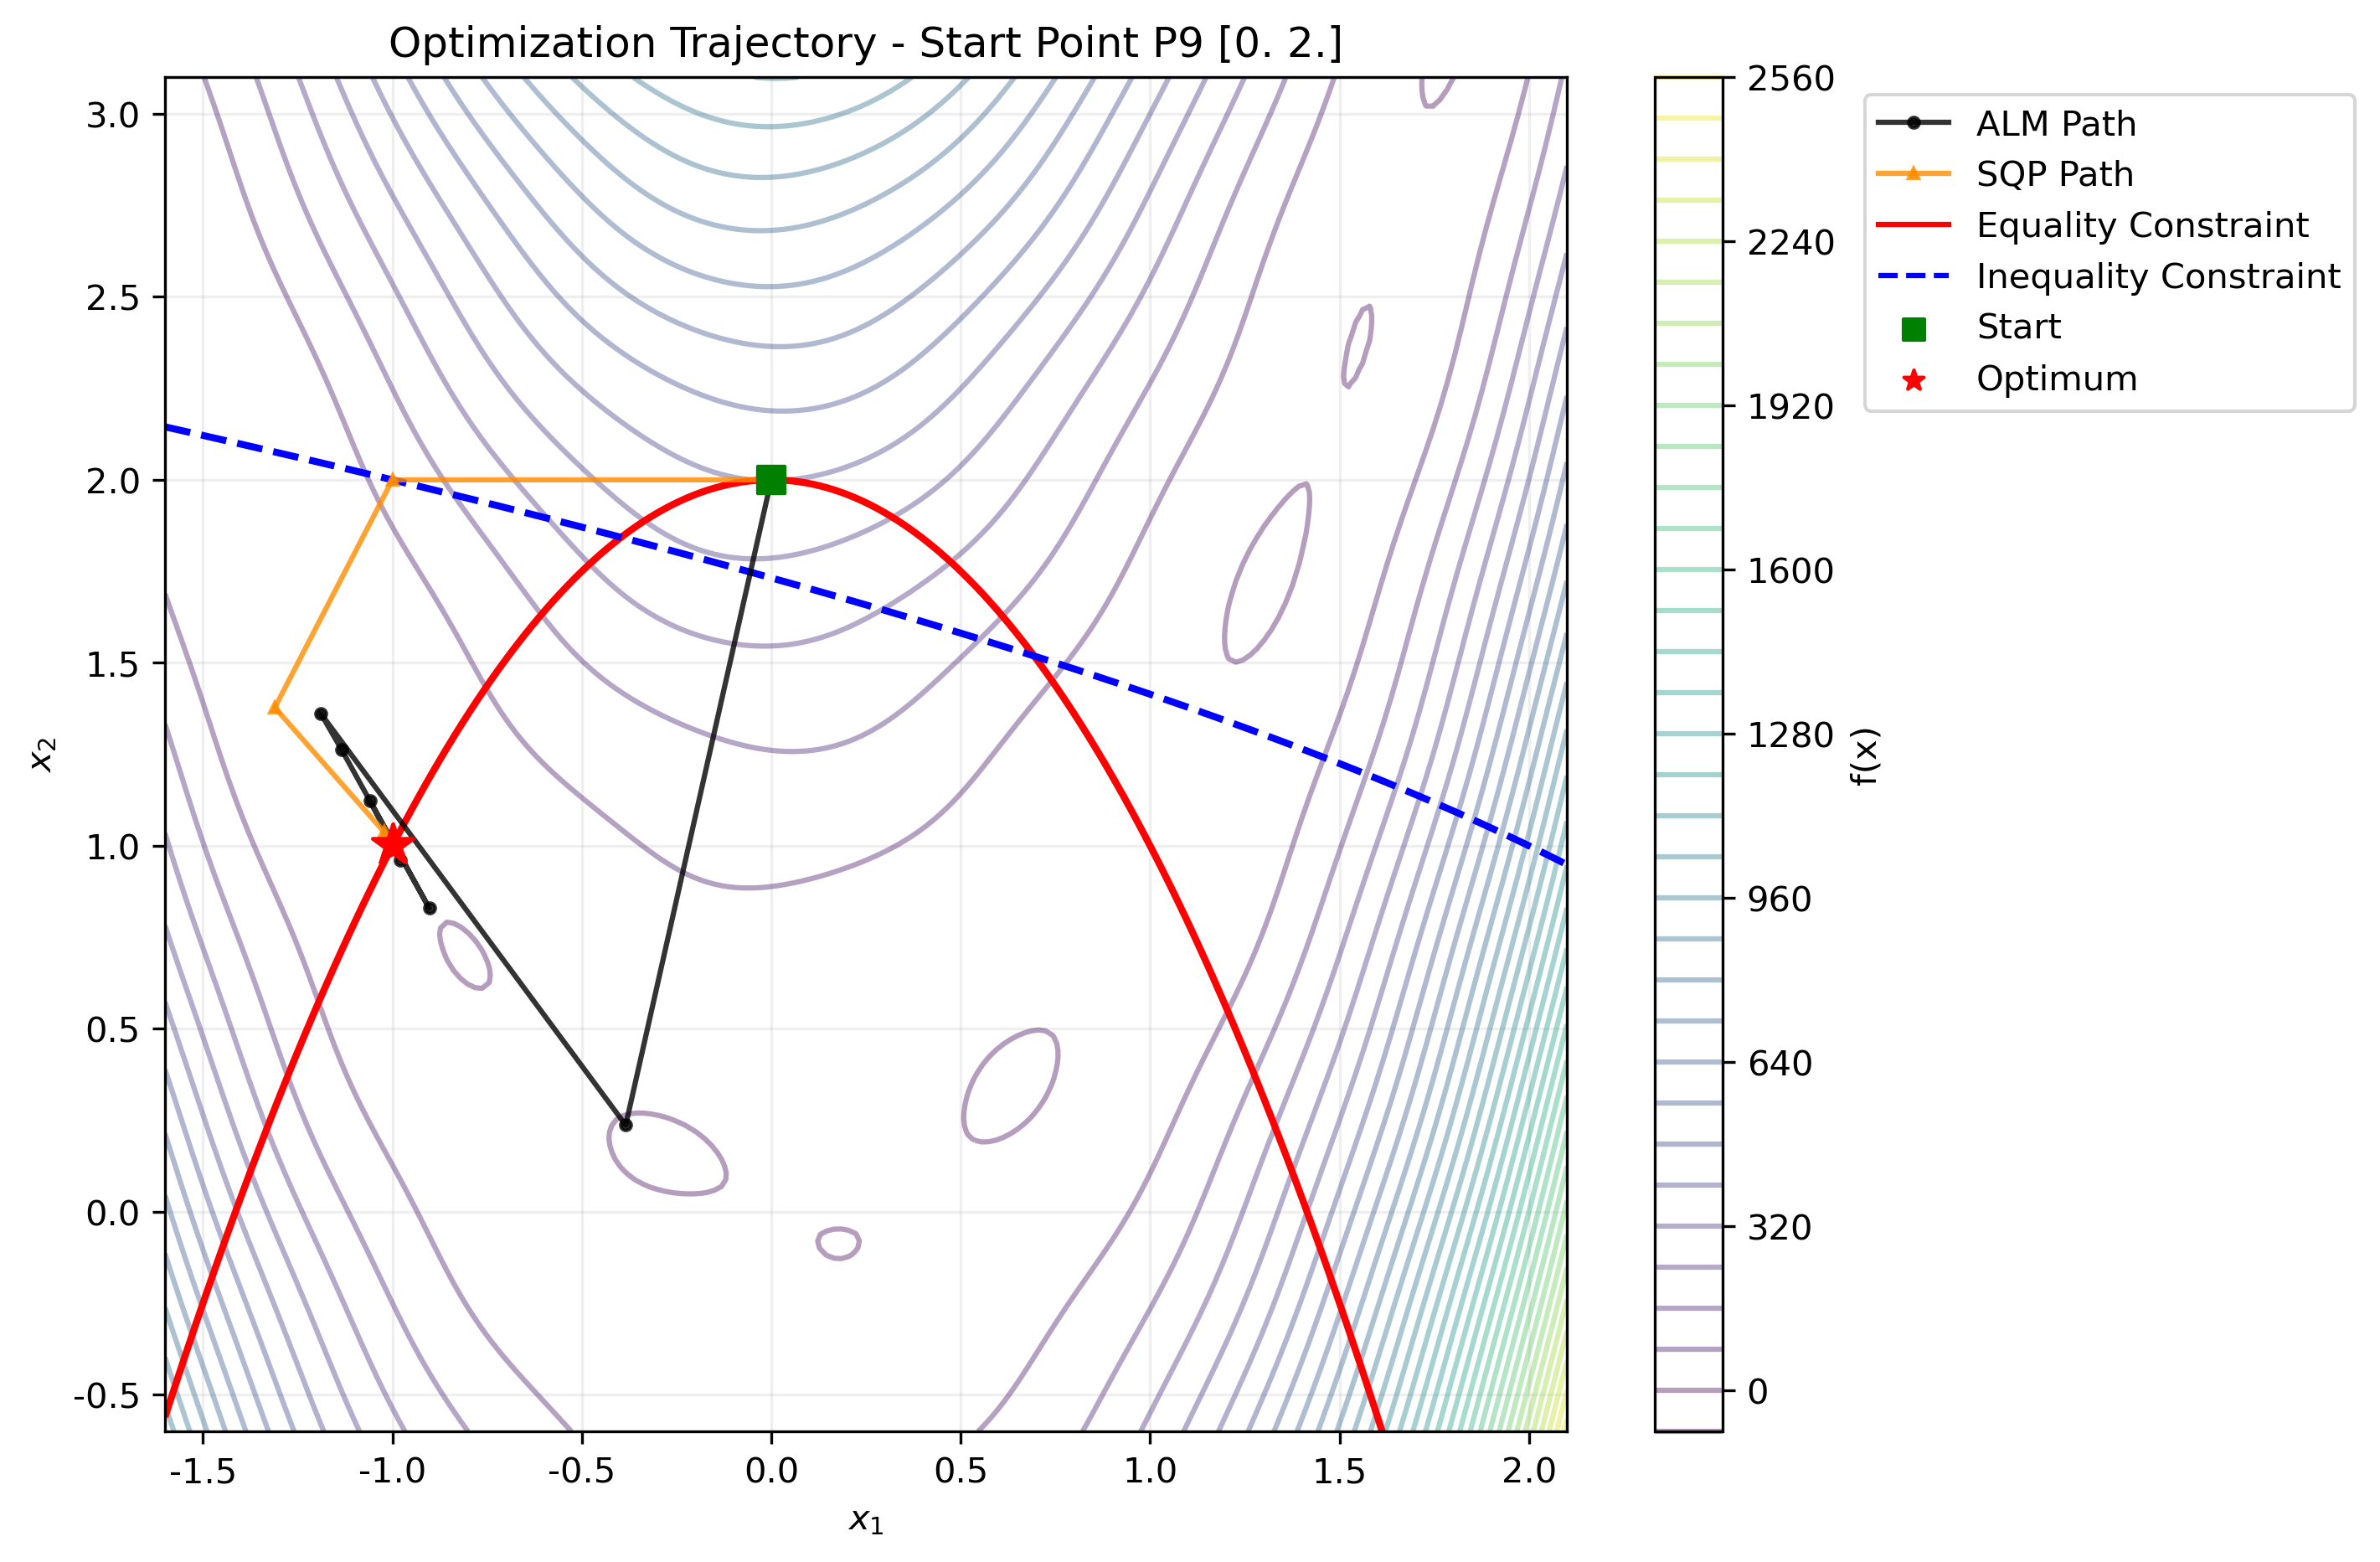
\includegraphics[width=\textwidth]{figures/path_2D_P9.png}
%         \caption{$P_9$: Parabola Vertex}
%     \end{subfigure}
%     \hfill
%     \begin{subfigure}[b]{0.48\textwidth}
%         \centering
%         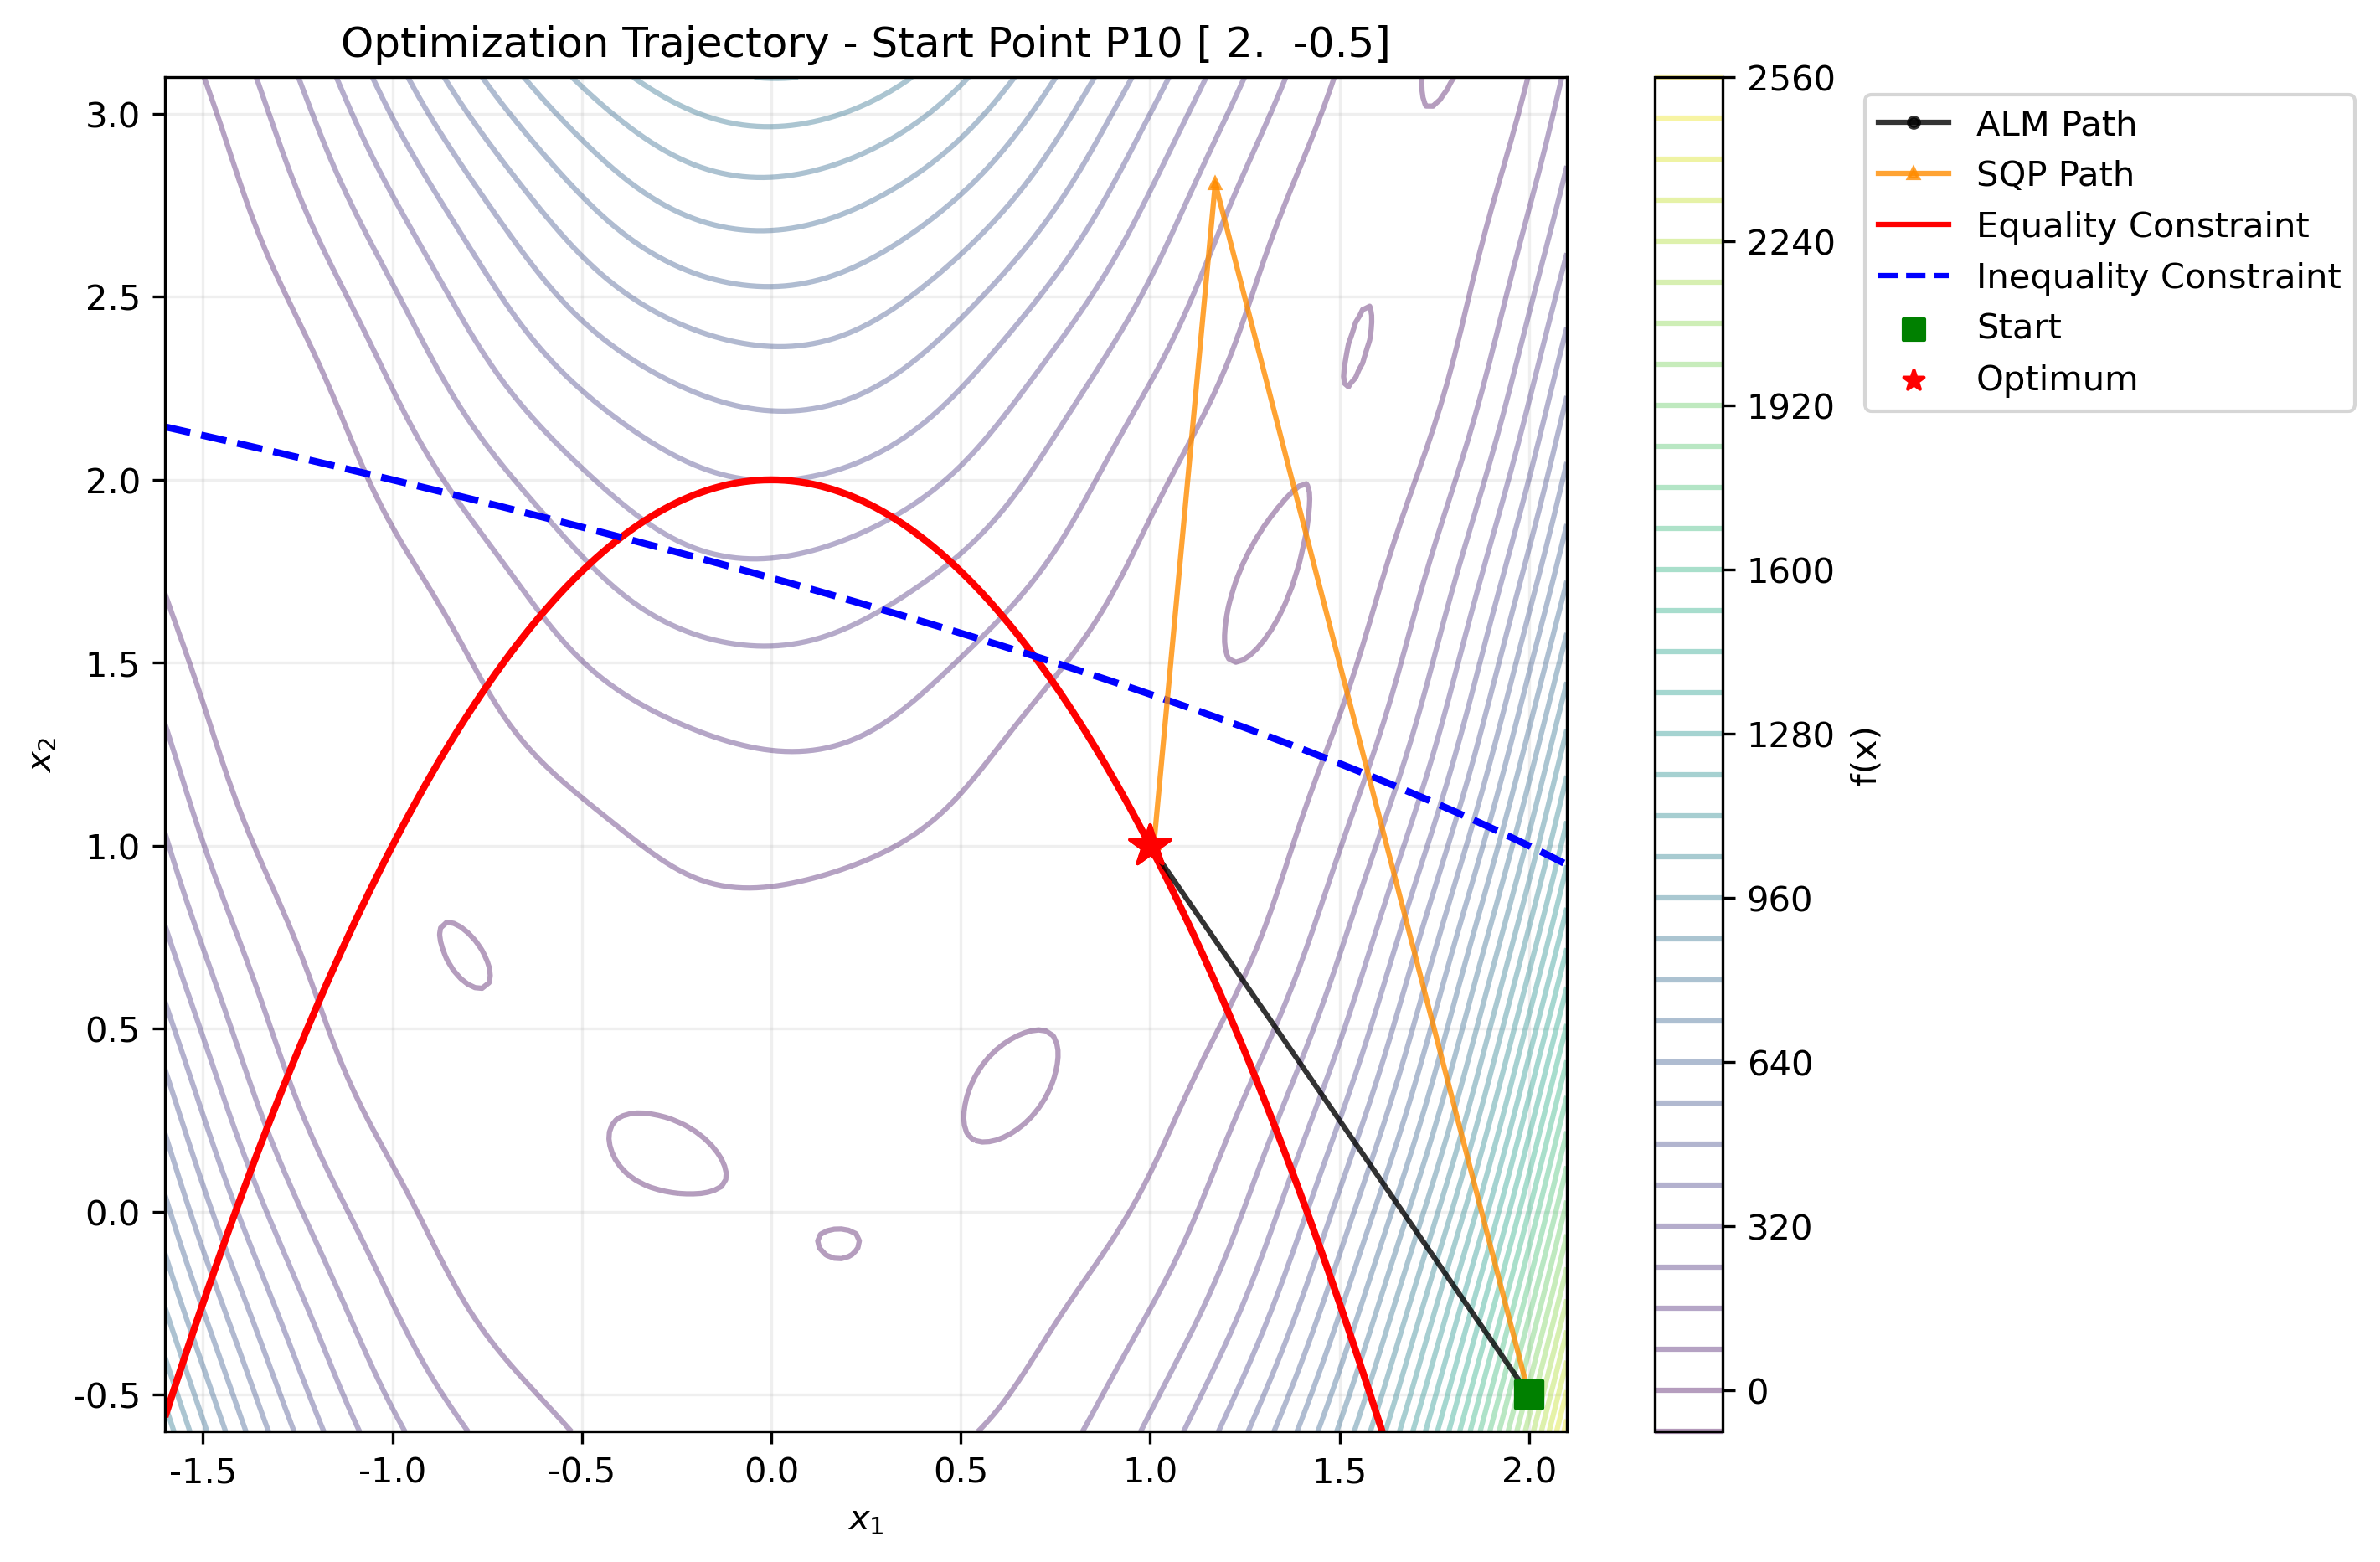
\includegraphics[width=\textwidth]{figures/path_2D_P10.png}
%         \caption{$P_{10}$: Corner Case}
%     \end{subfigure}
    
%     \caption{2D Modified Rosenbrock 问题下 ALM (黑线) 与 SQP (橙线) 的完整迭代轨迹对比（$P_1 - P_{10}$）。背景等高线表示目标函数，红色曲线为等式约束。}
%     \label{fig:app_all_paths}
% \end{figure}

% --- 第一页 (P1 - P6) ---
\begin{figure}[p]
    \centering
    % 第一行 P1, P2
    \begin{subfigure}[b]{0.48\textwidth}
        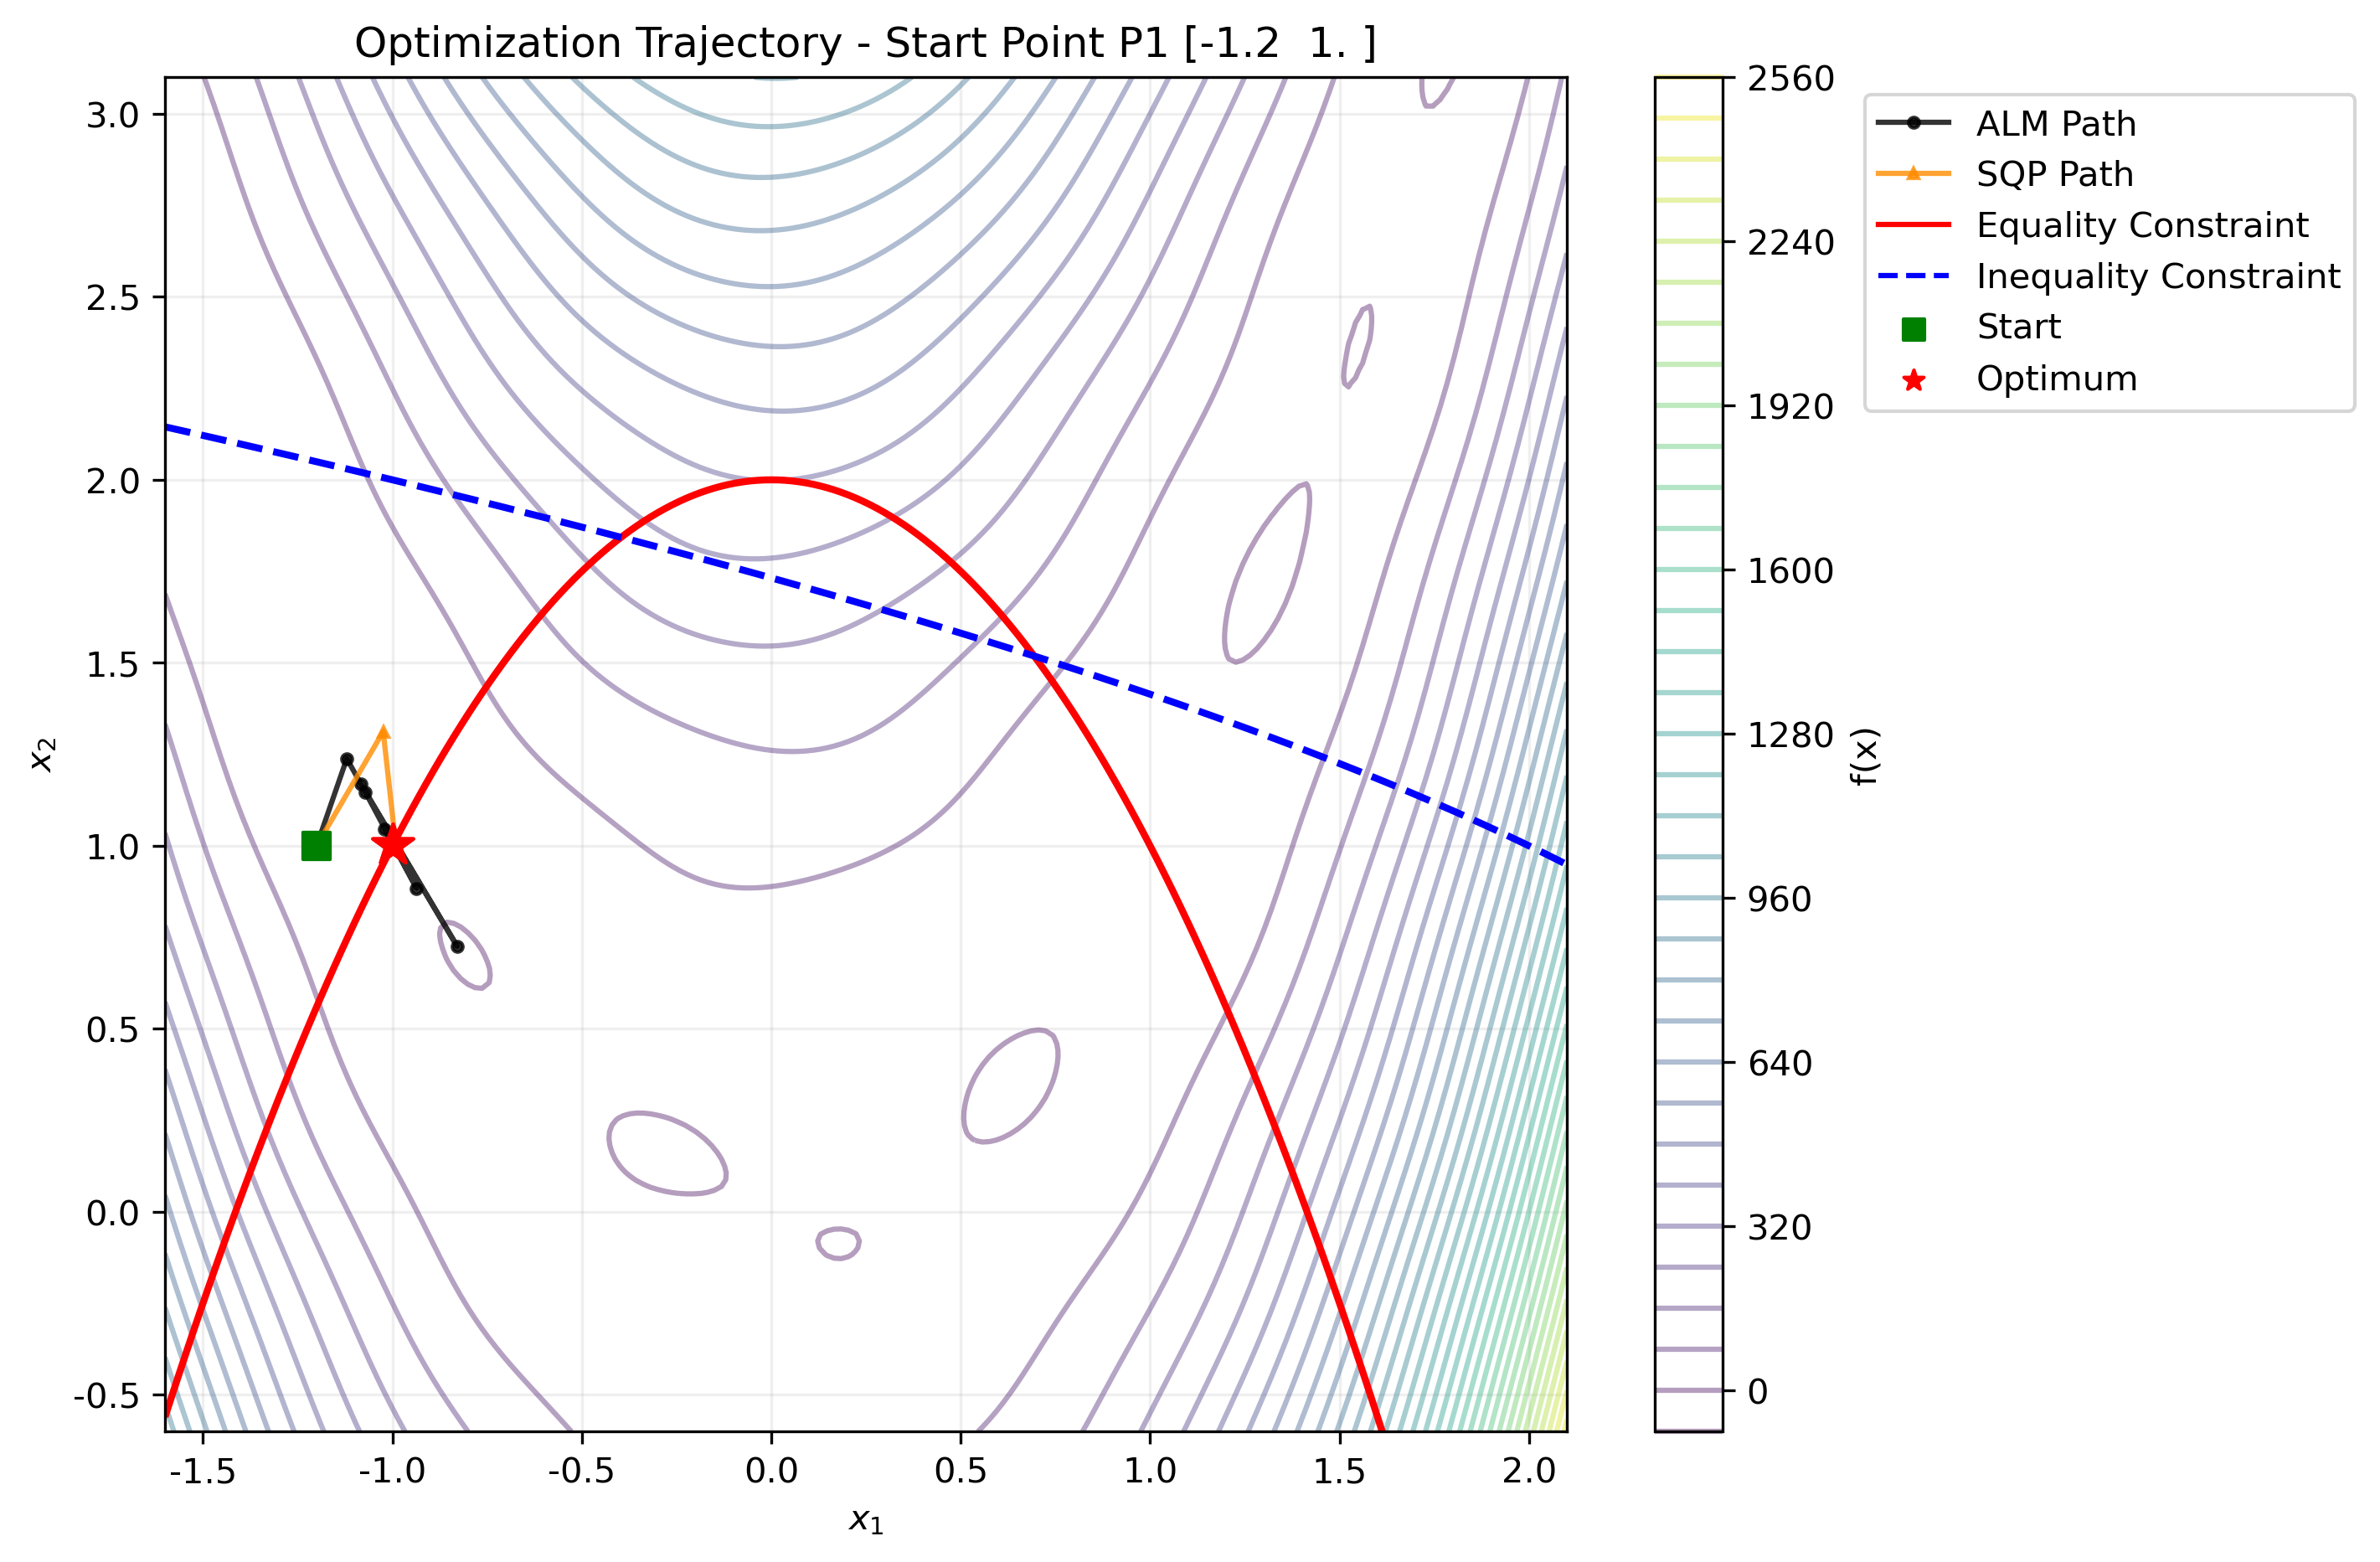
\includegraphics[width=\textwidth]{figures/path_2D_P1.png} \caption{$P_1$}
    \end{subfigure}
    \hfill
    \begin{subfigure}[b]{0.48\textwidth}
        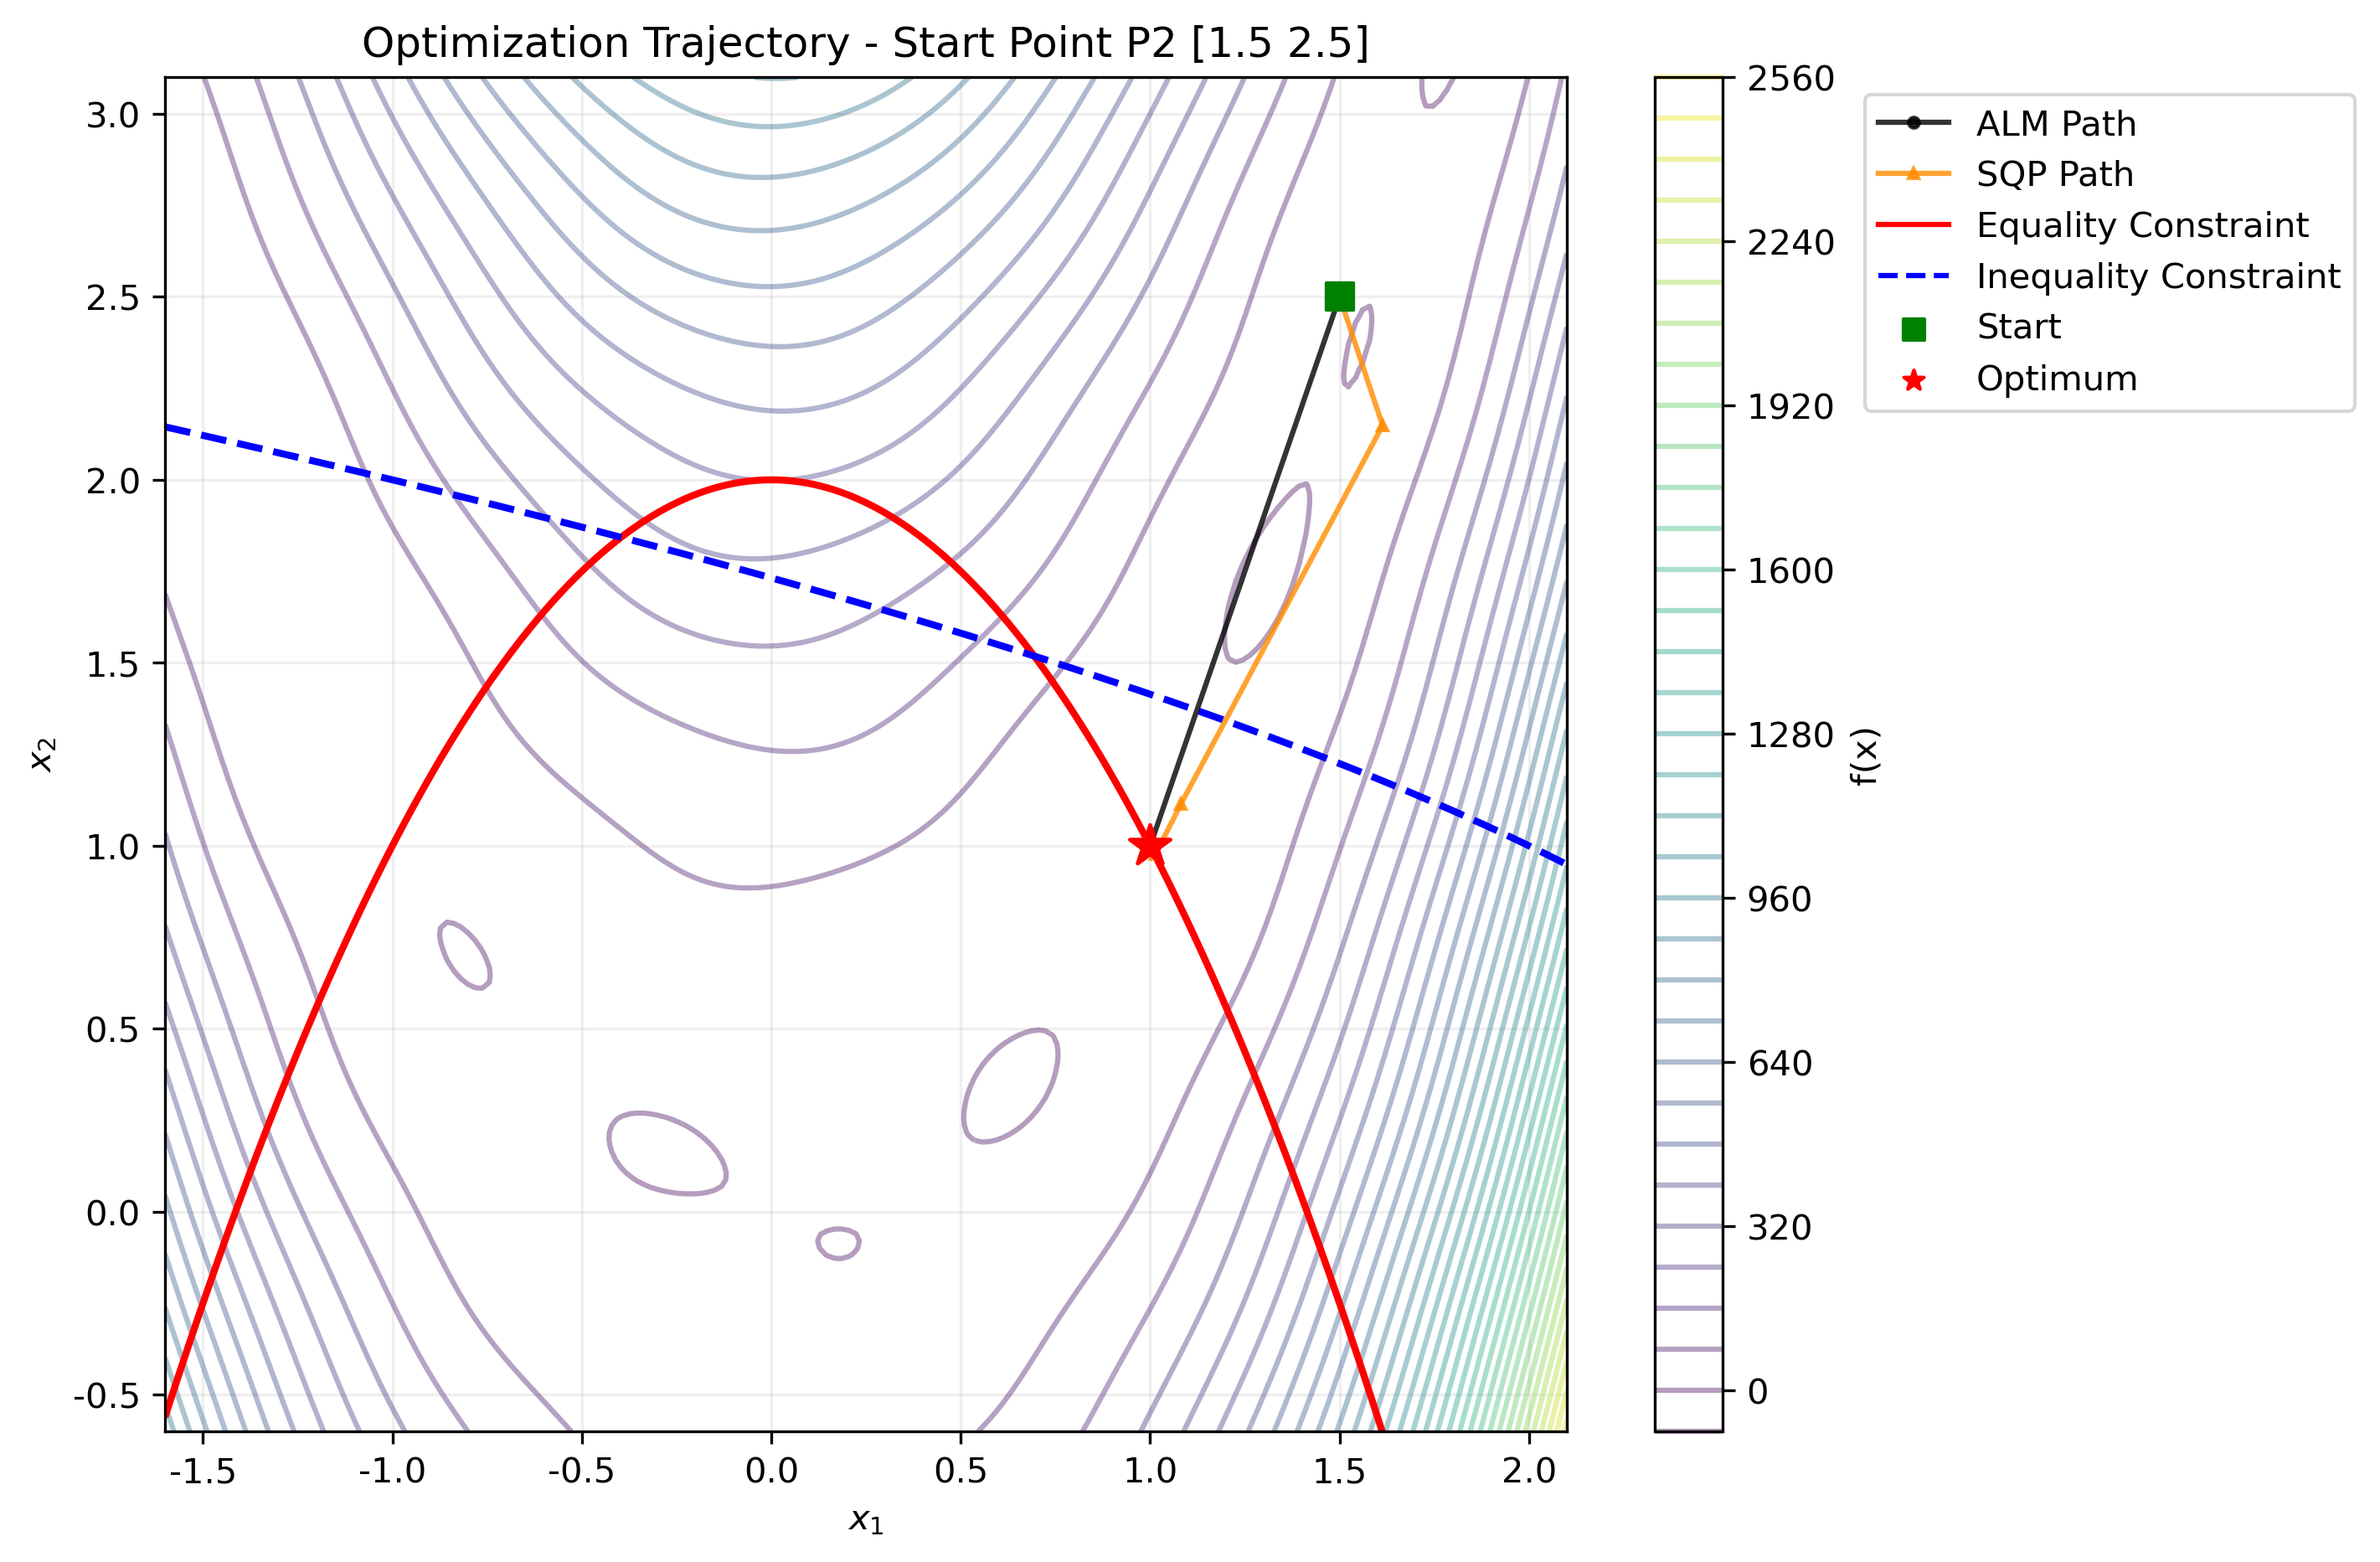
\includegraphics[width=\textwidth]{figures/path_2D_P2.png} \caption{$P_2$}
    \end{subfigure}
    
    \vspace{1em}
    
    % 第二行 P3, P4
    \begin{subfigure}[b]{0.48\textwidth}
        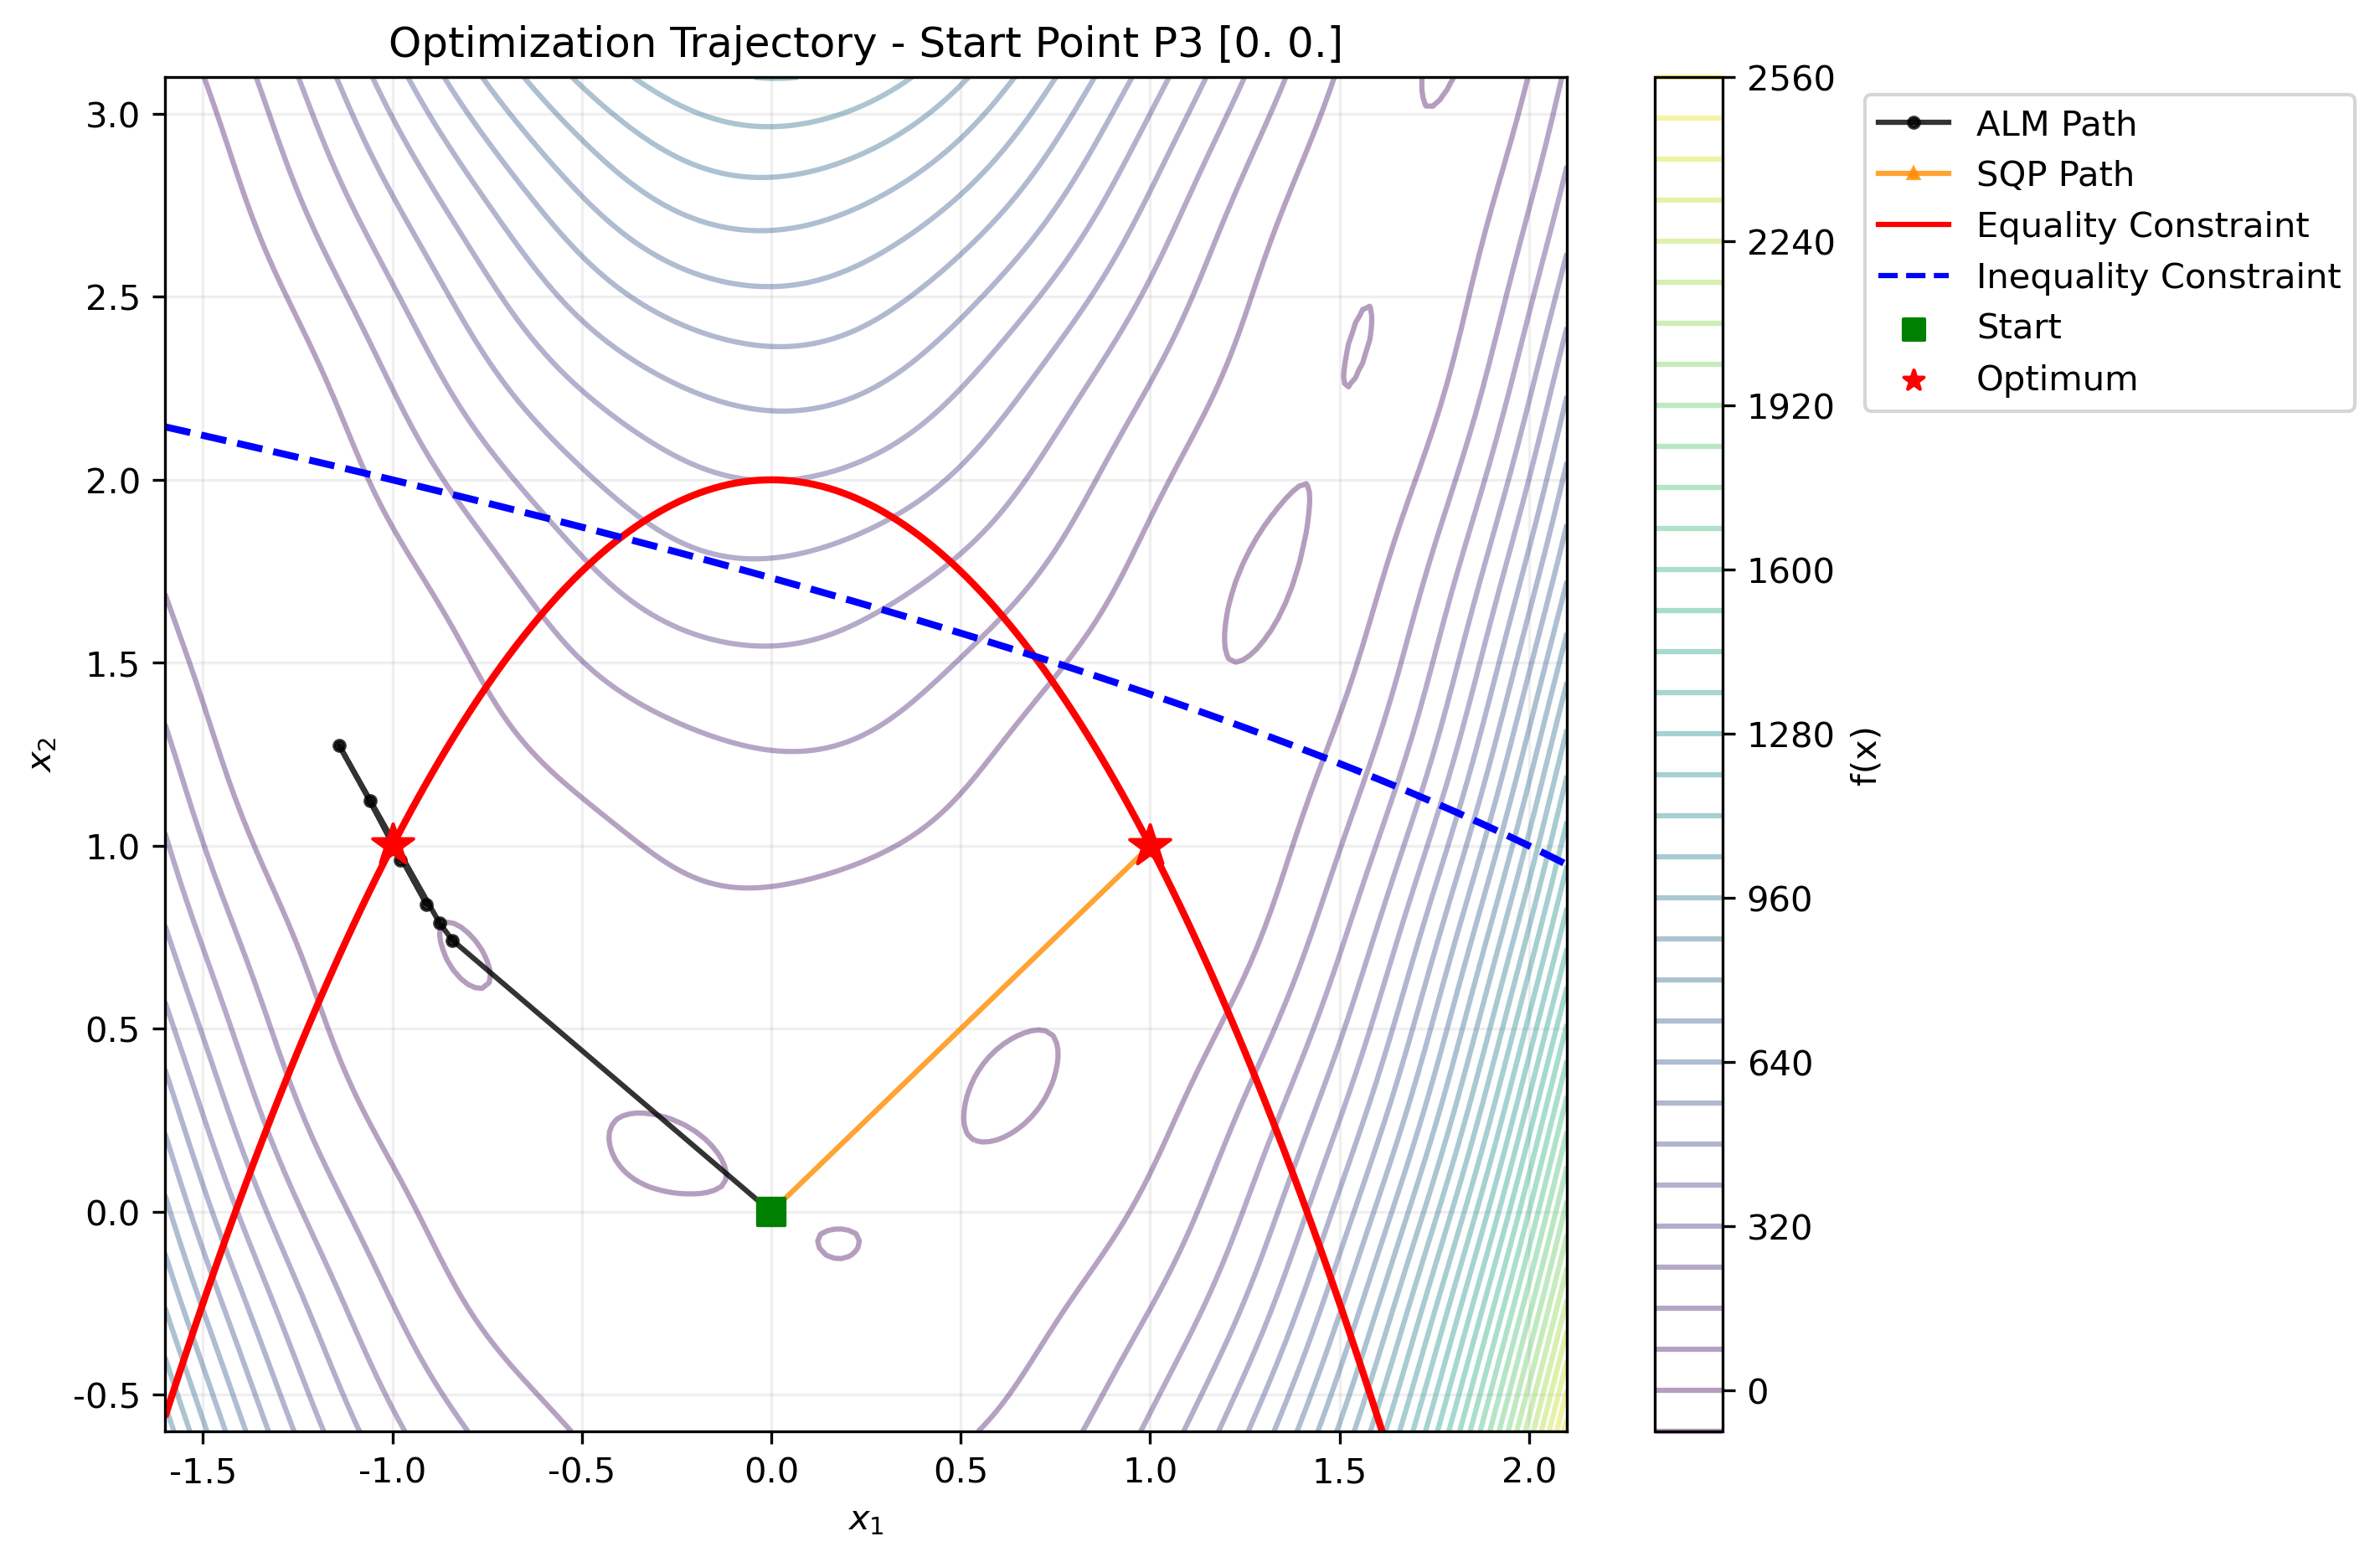
\includegraphics[width=\textwidth]{figures/path_2D_P3.png} \caption{$P_3$}
    \end{subfigure}
    \hfill
    \begin{subfigure}[b]{0.48\textwidth}
        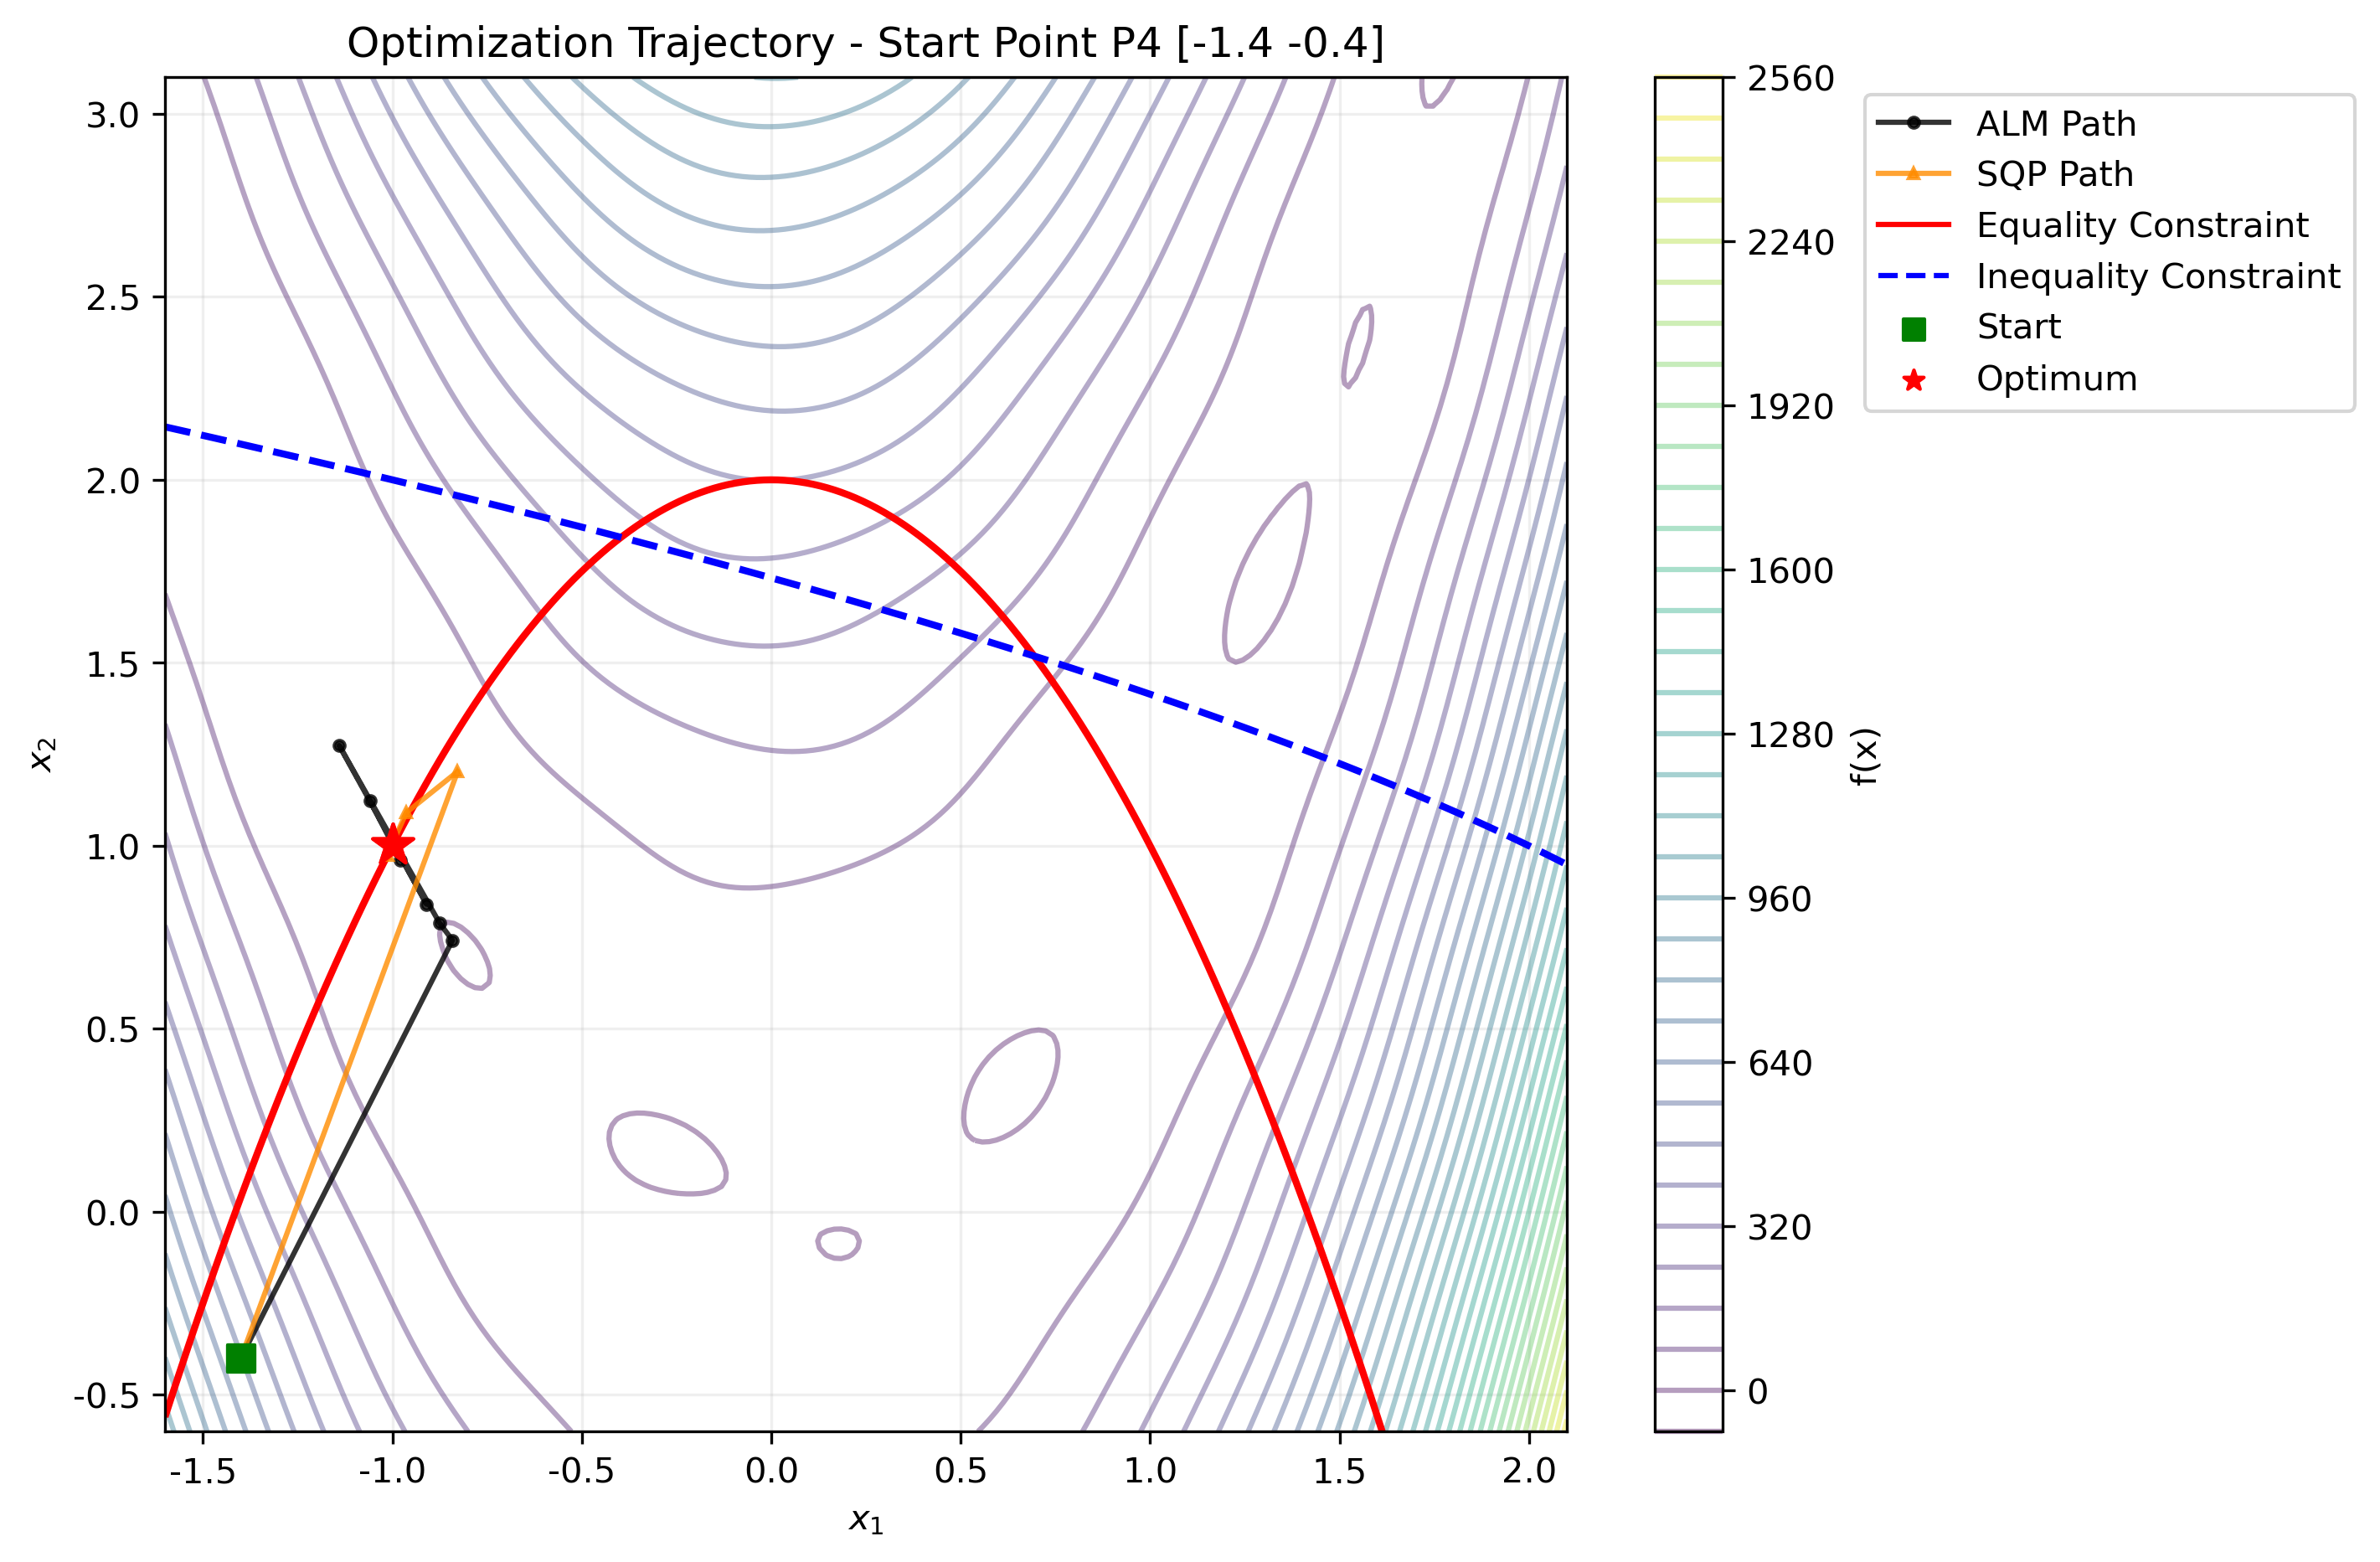
\includegraphics[width=\textwidth]{figures/path_2D_P4.png} \caption{$P_4$}
    \end{subfigure}
    
    \vspace{1em}
    
    % 第三行 P5, P6
    \begin{subfigure}[b]{0.48\textwidth}
        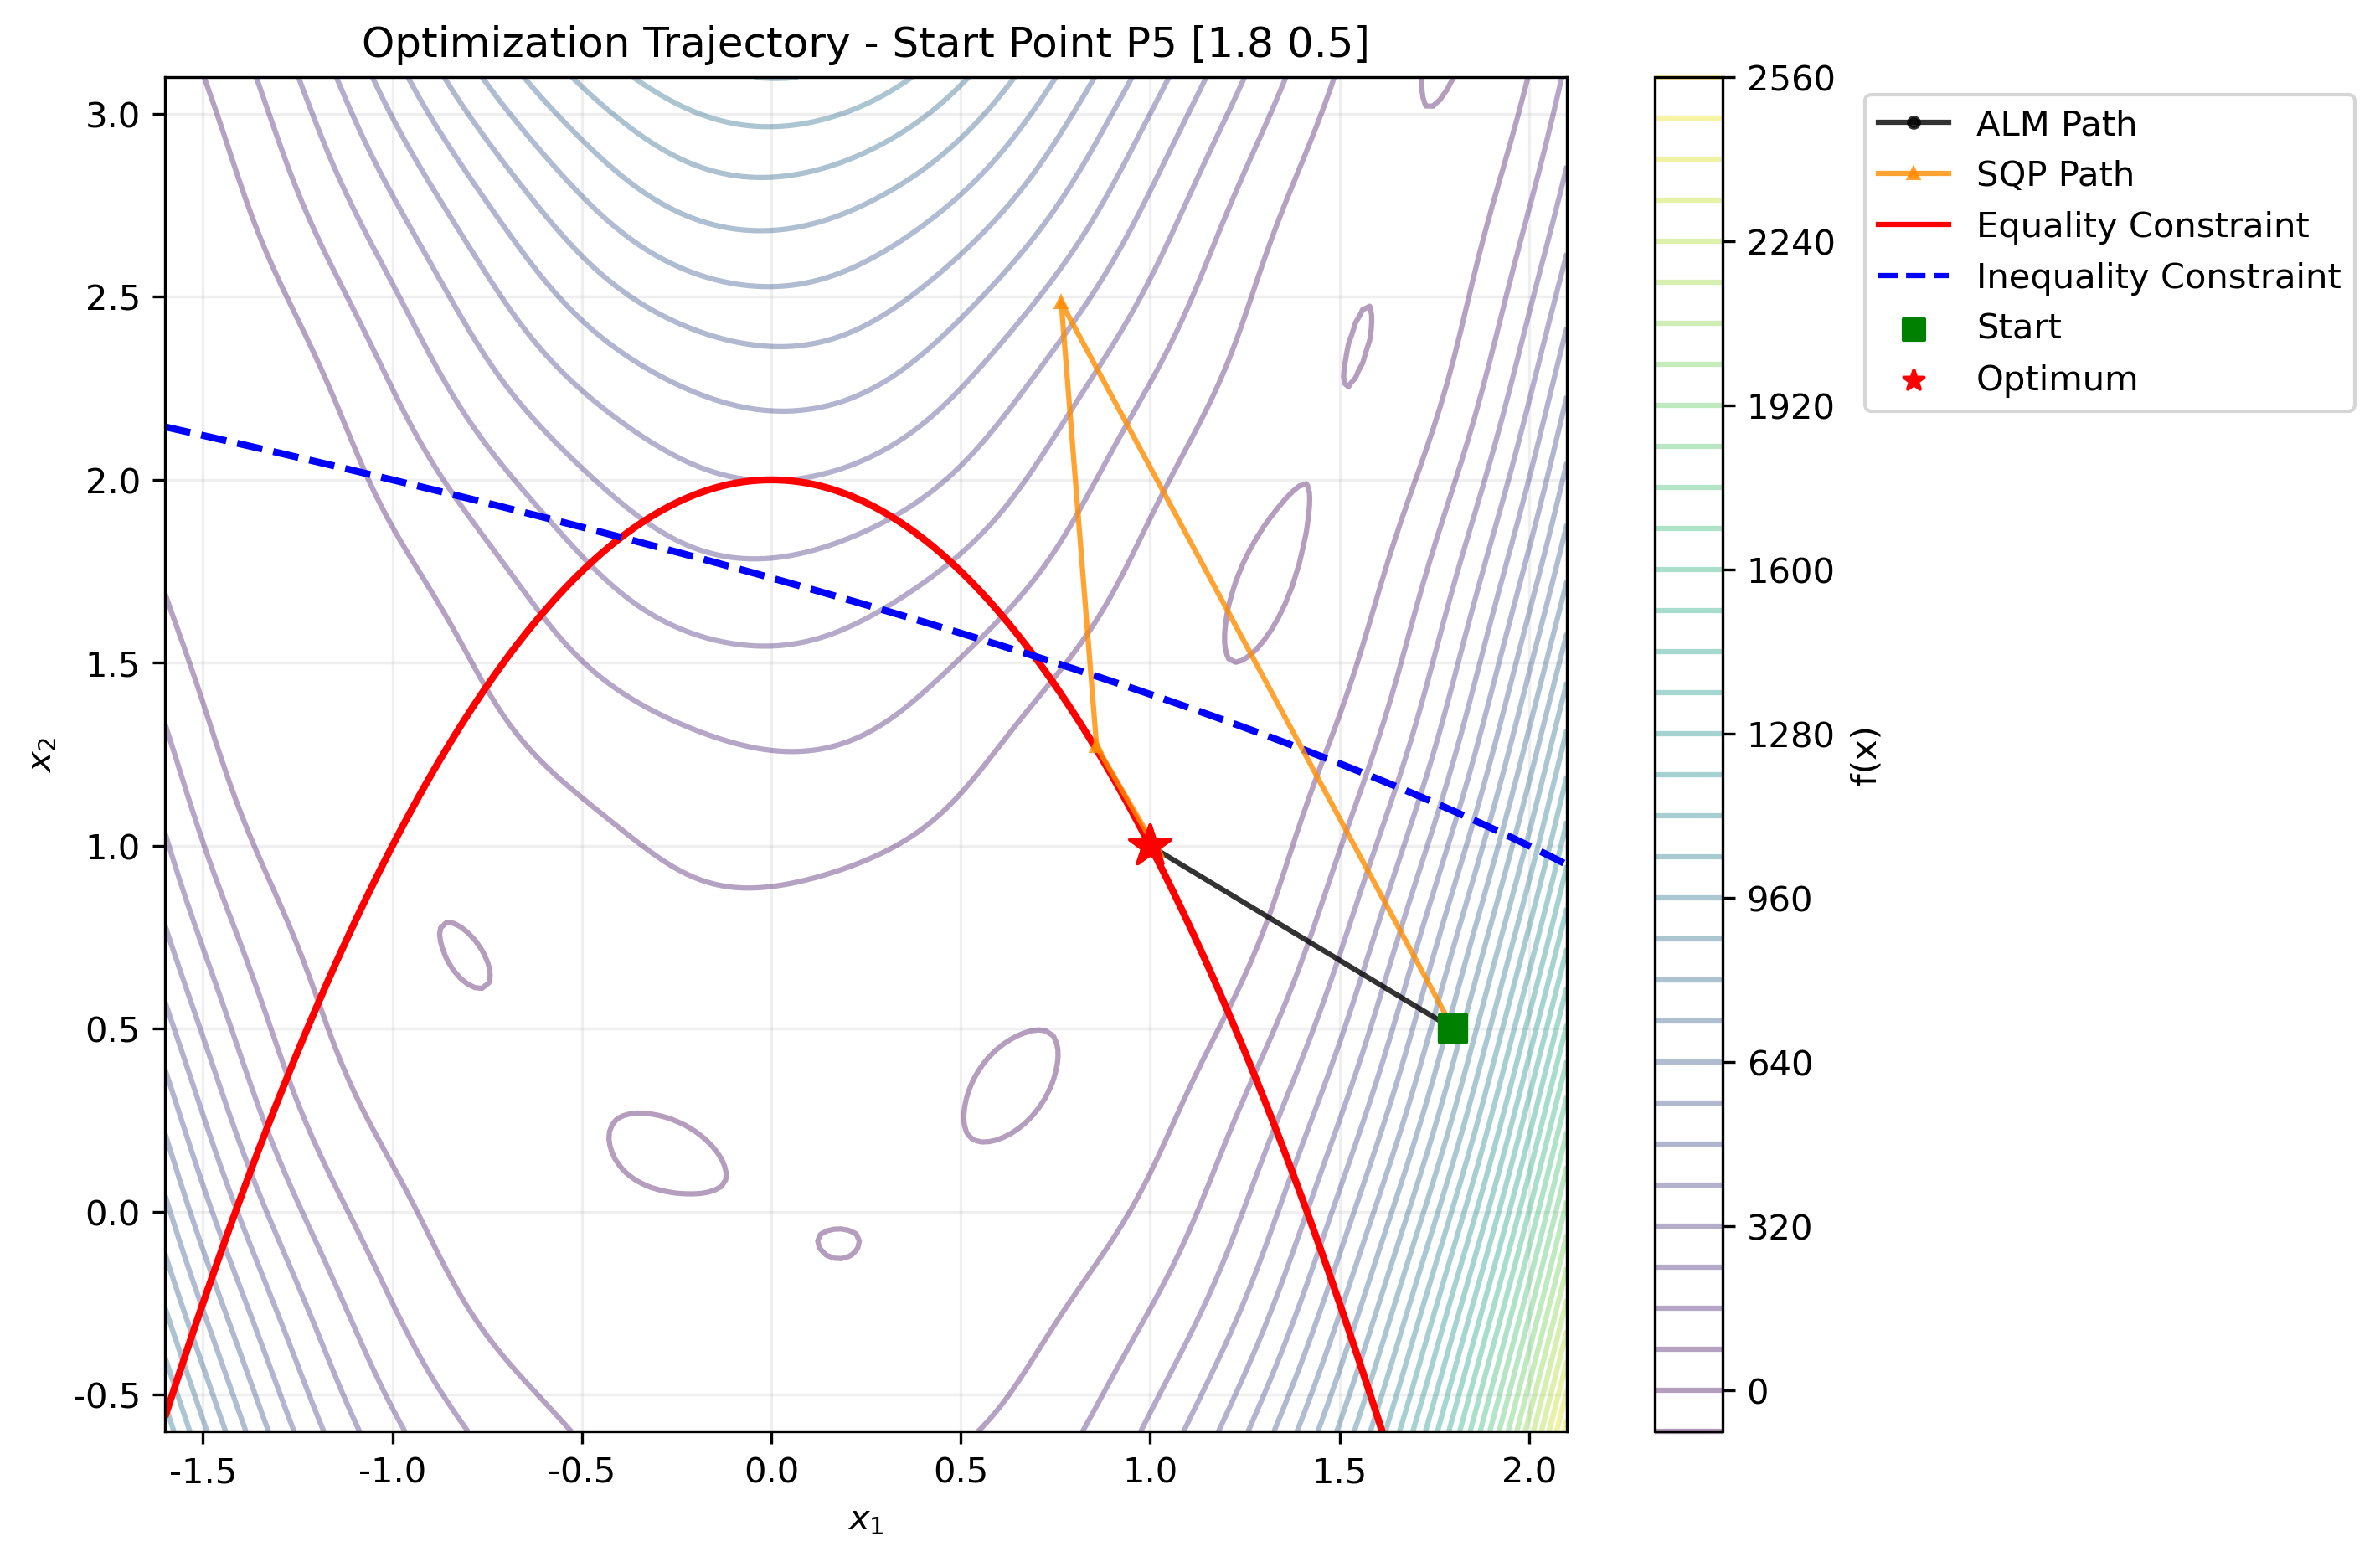
\includegraphics[width=\textwidth]{figures/path_2D_P5.png} \caption{$P_5$}
    \end{subfigure}
    \hfill
    \begin{subfigure}[b]{0.48\textwidth}
        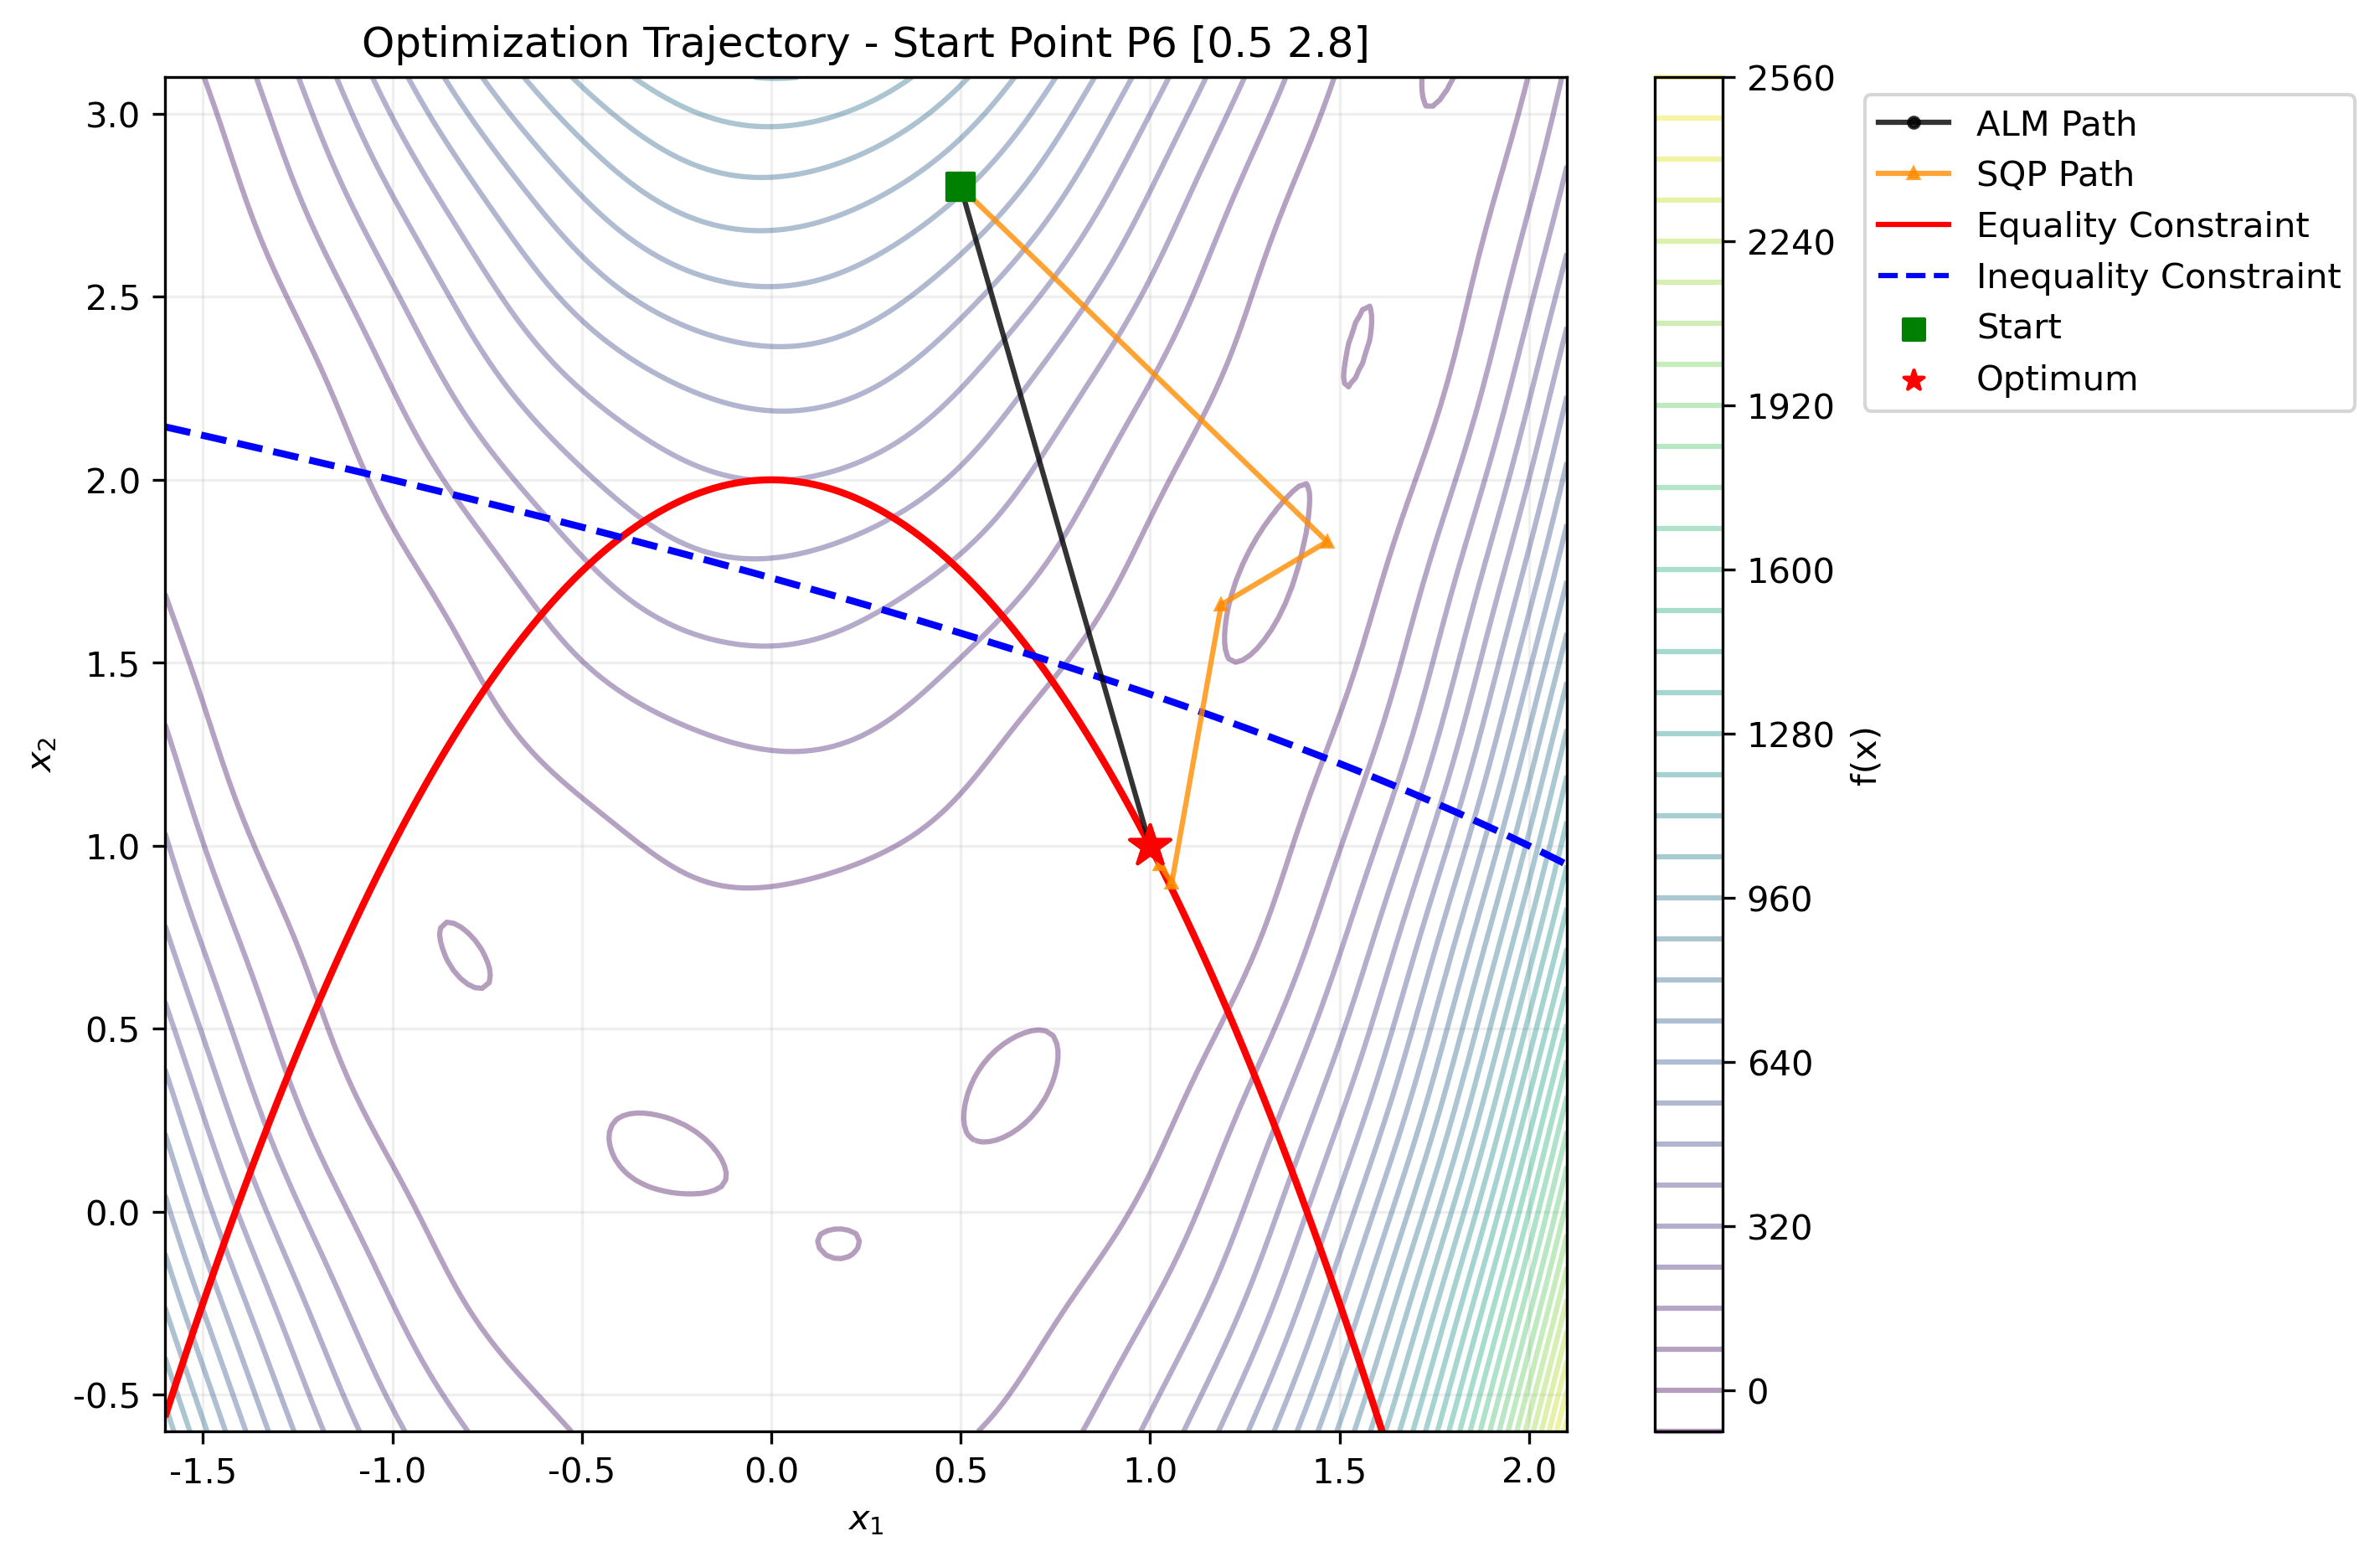
\includegraphics[width=\textwidth]{figures/path_2D_P6.png} \caption{$P_6$}
    \end{subfigure}
    
    % 这里写主标题
    \caption{2D Modified Rosenbrock 问题迭代轨迹对比（部分）。}
    \label{fig:app_all_paths}
\end{figure}

\clearpage % 强制换页

% --- 第二页 (P7 - P10) ---
\begin{figure}[t] % 使用 [t] 让图片在页面顶部
    \ContinuedFloat % <--- 关键命令：保持图号连续（例如还是 Figure 1）
    \centering
    
    % 第四行 P7, P8
    \begin{subfigure}[b]{0.48\textwidth}
        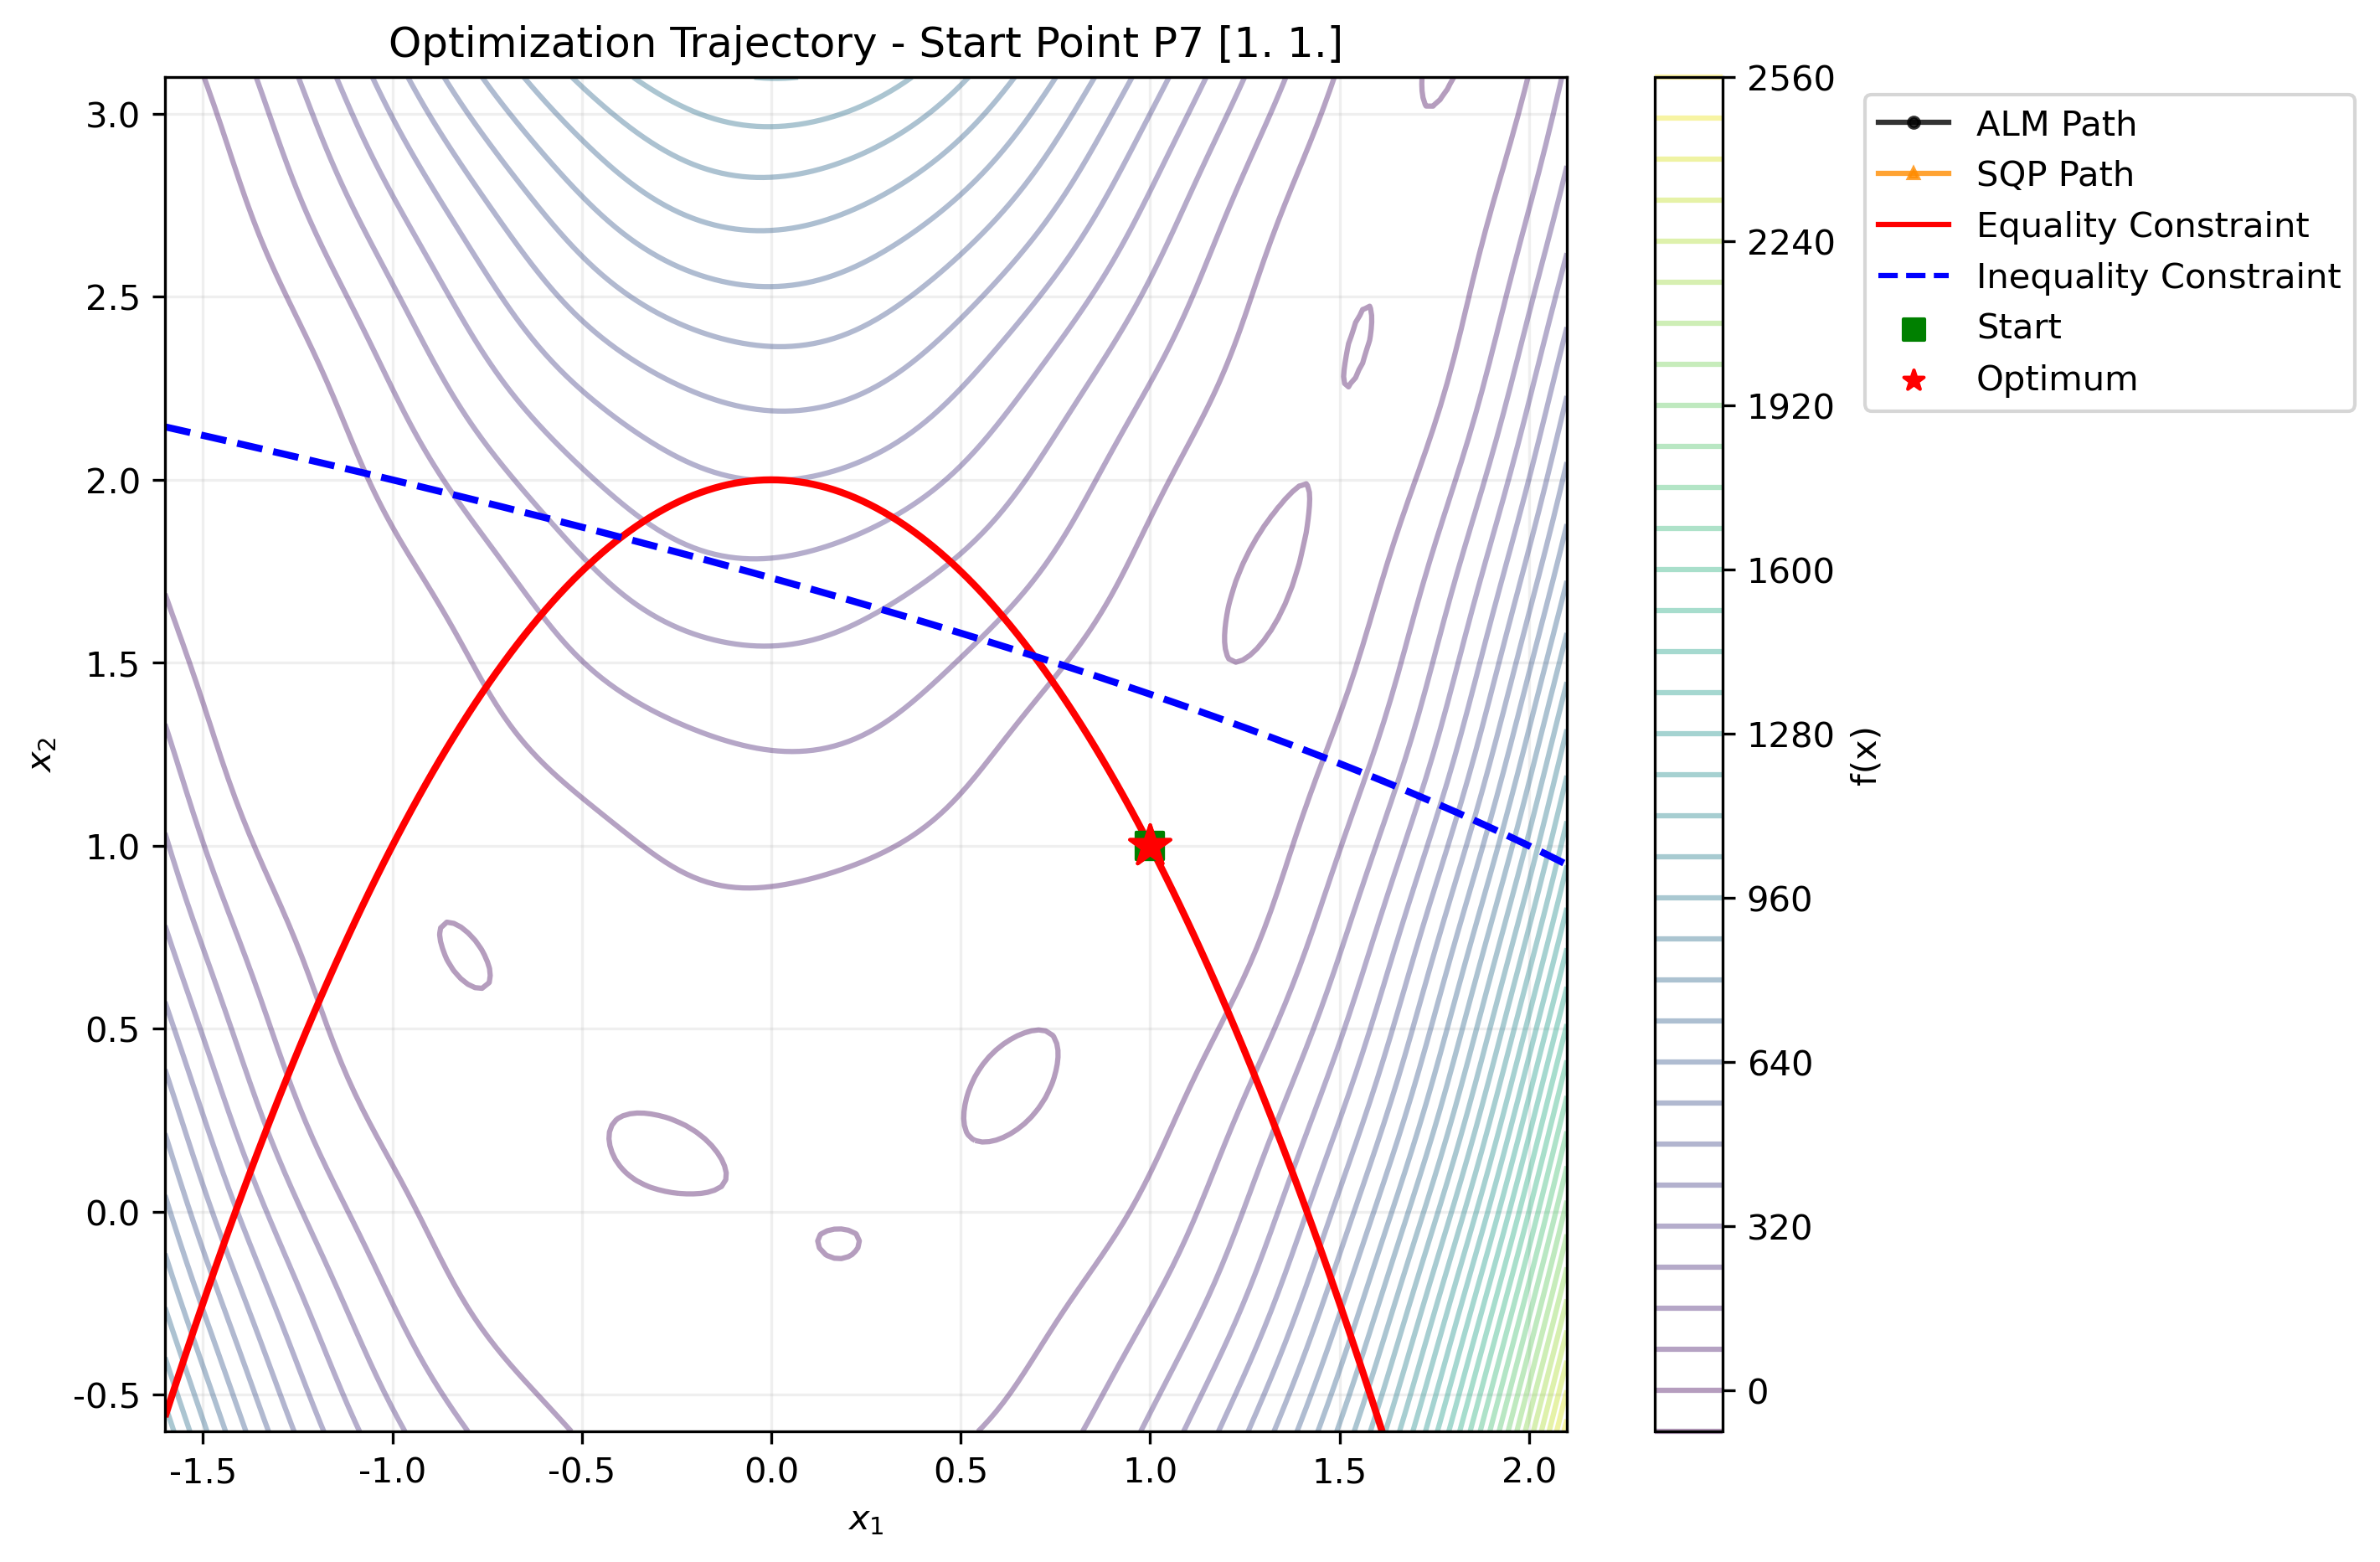
\includegraphics[width=\textwidth]{figures/path_2D_P7.png} \caption{$P_7$}
    \end{subfigure}
    \hfill
    \begin{subfigure}[b]{0.48\textwidth}
        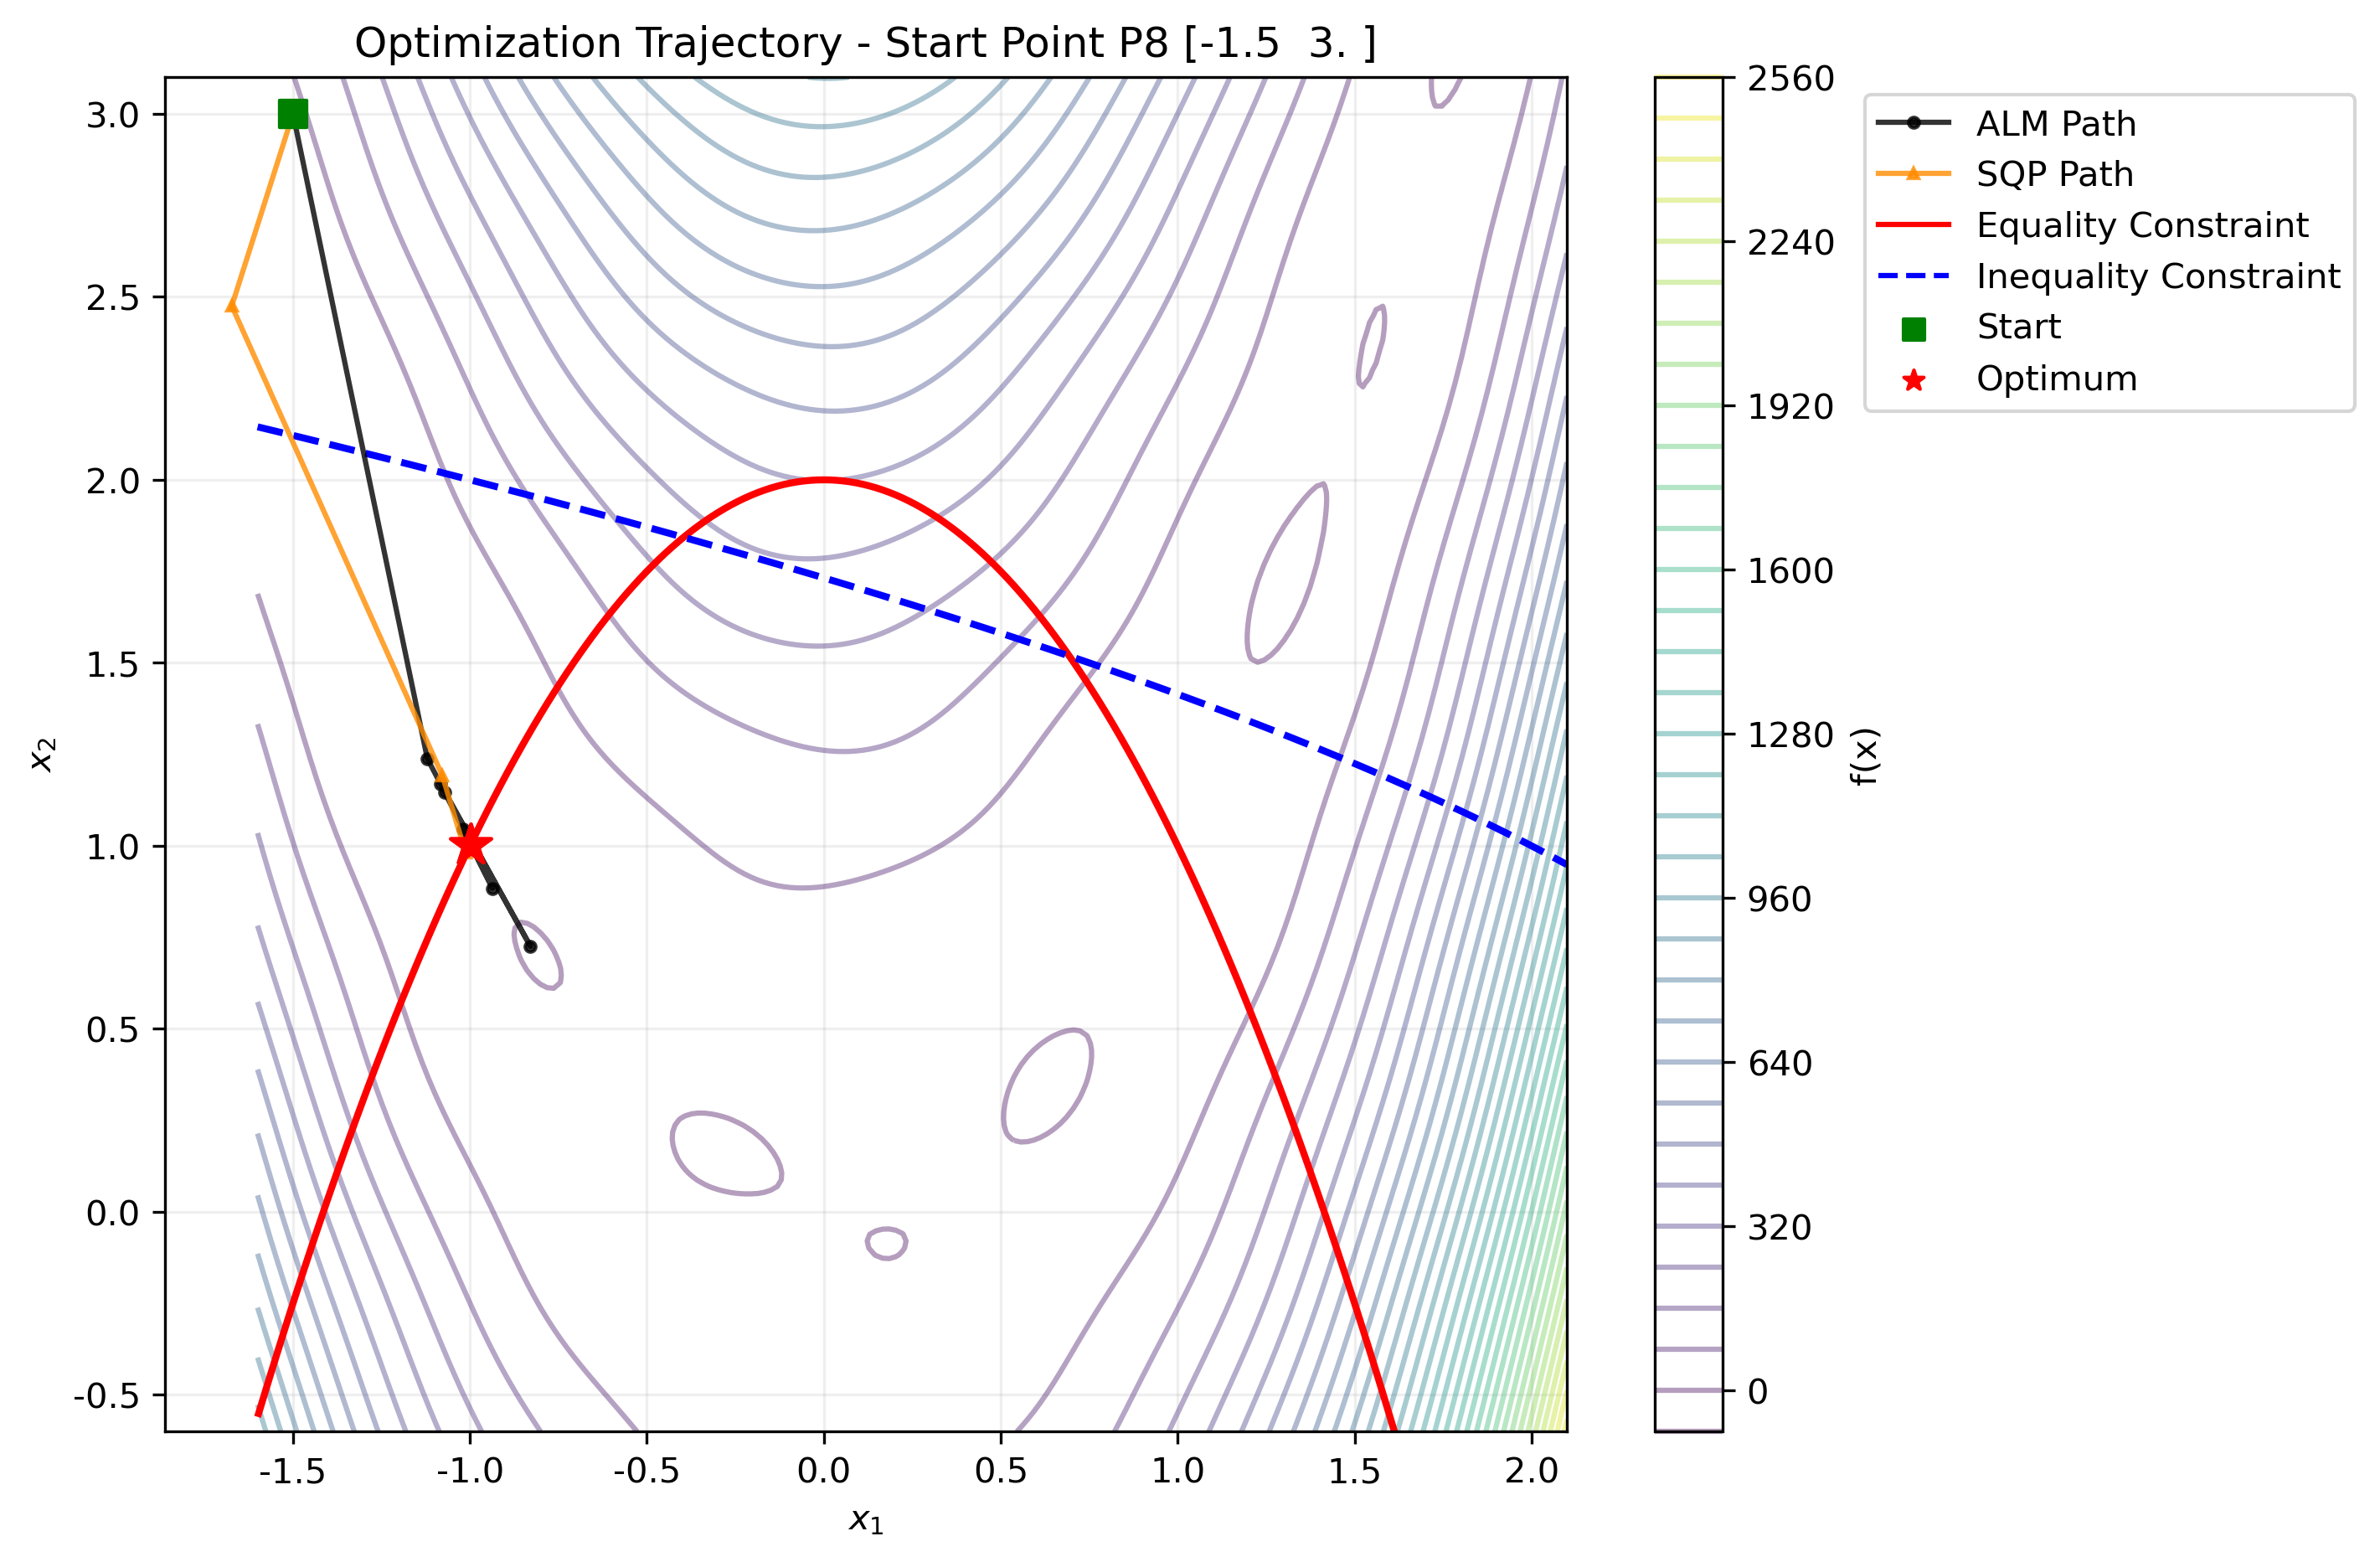
\includegraphics[width=\textwidth]{figures/path_2D_P8.png} \caption{$P_8$}
    \end{subfigure}
    
    \vspace{1em}
    
    % 第五行 P9, P10
    \begin{subfigure}[b]{0.48\textwidth}
        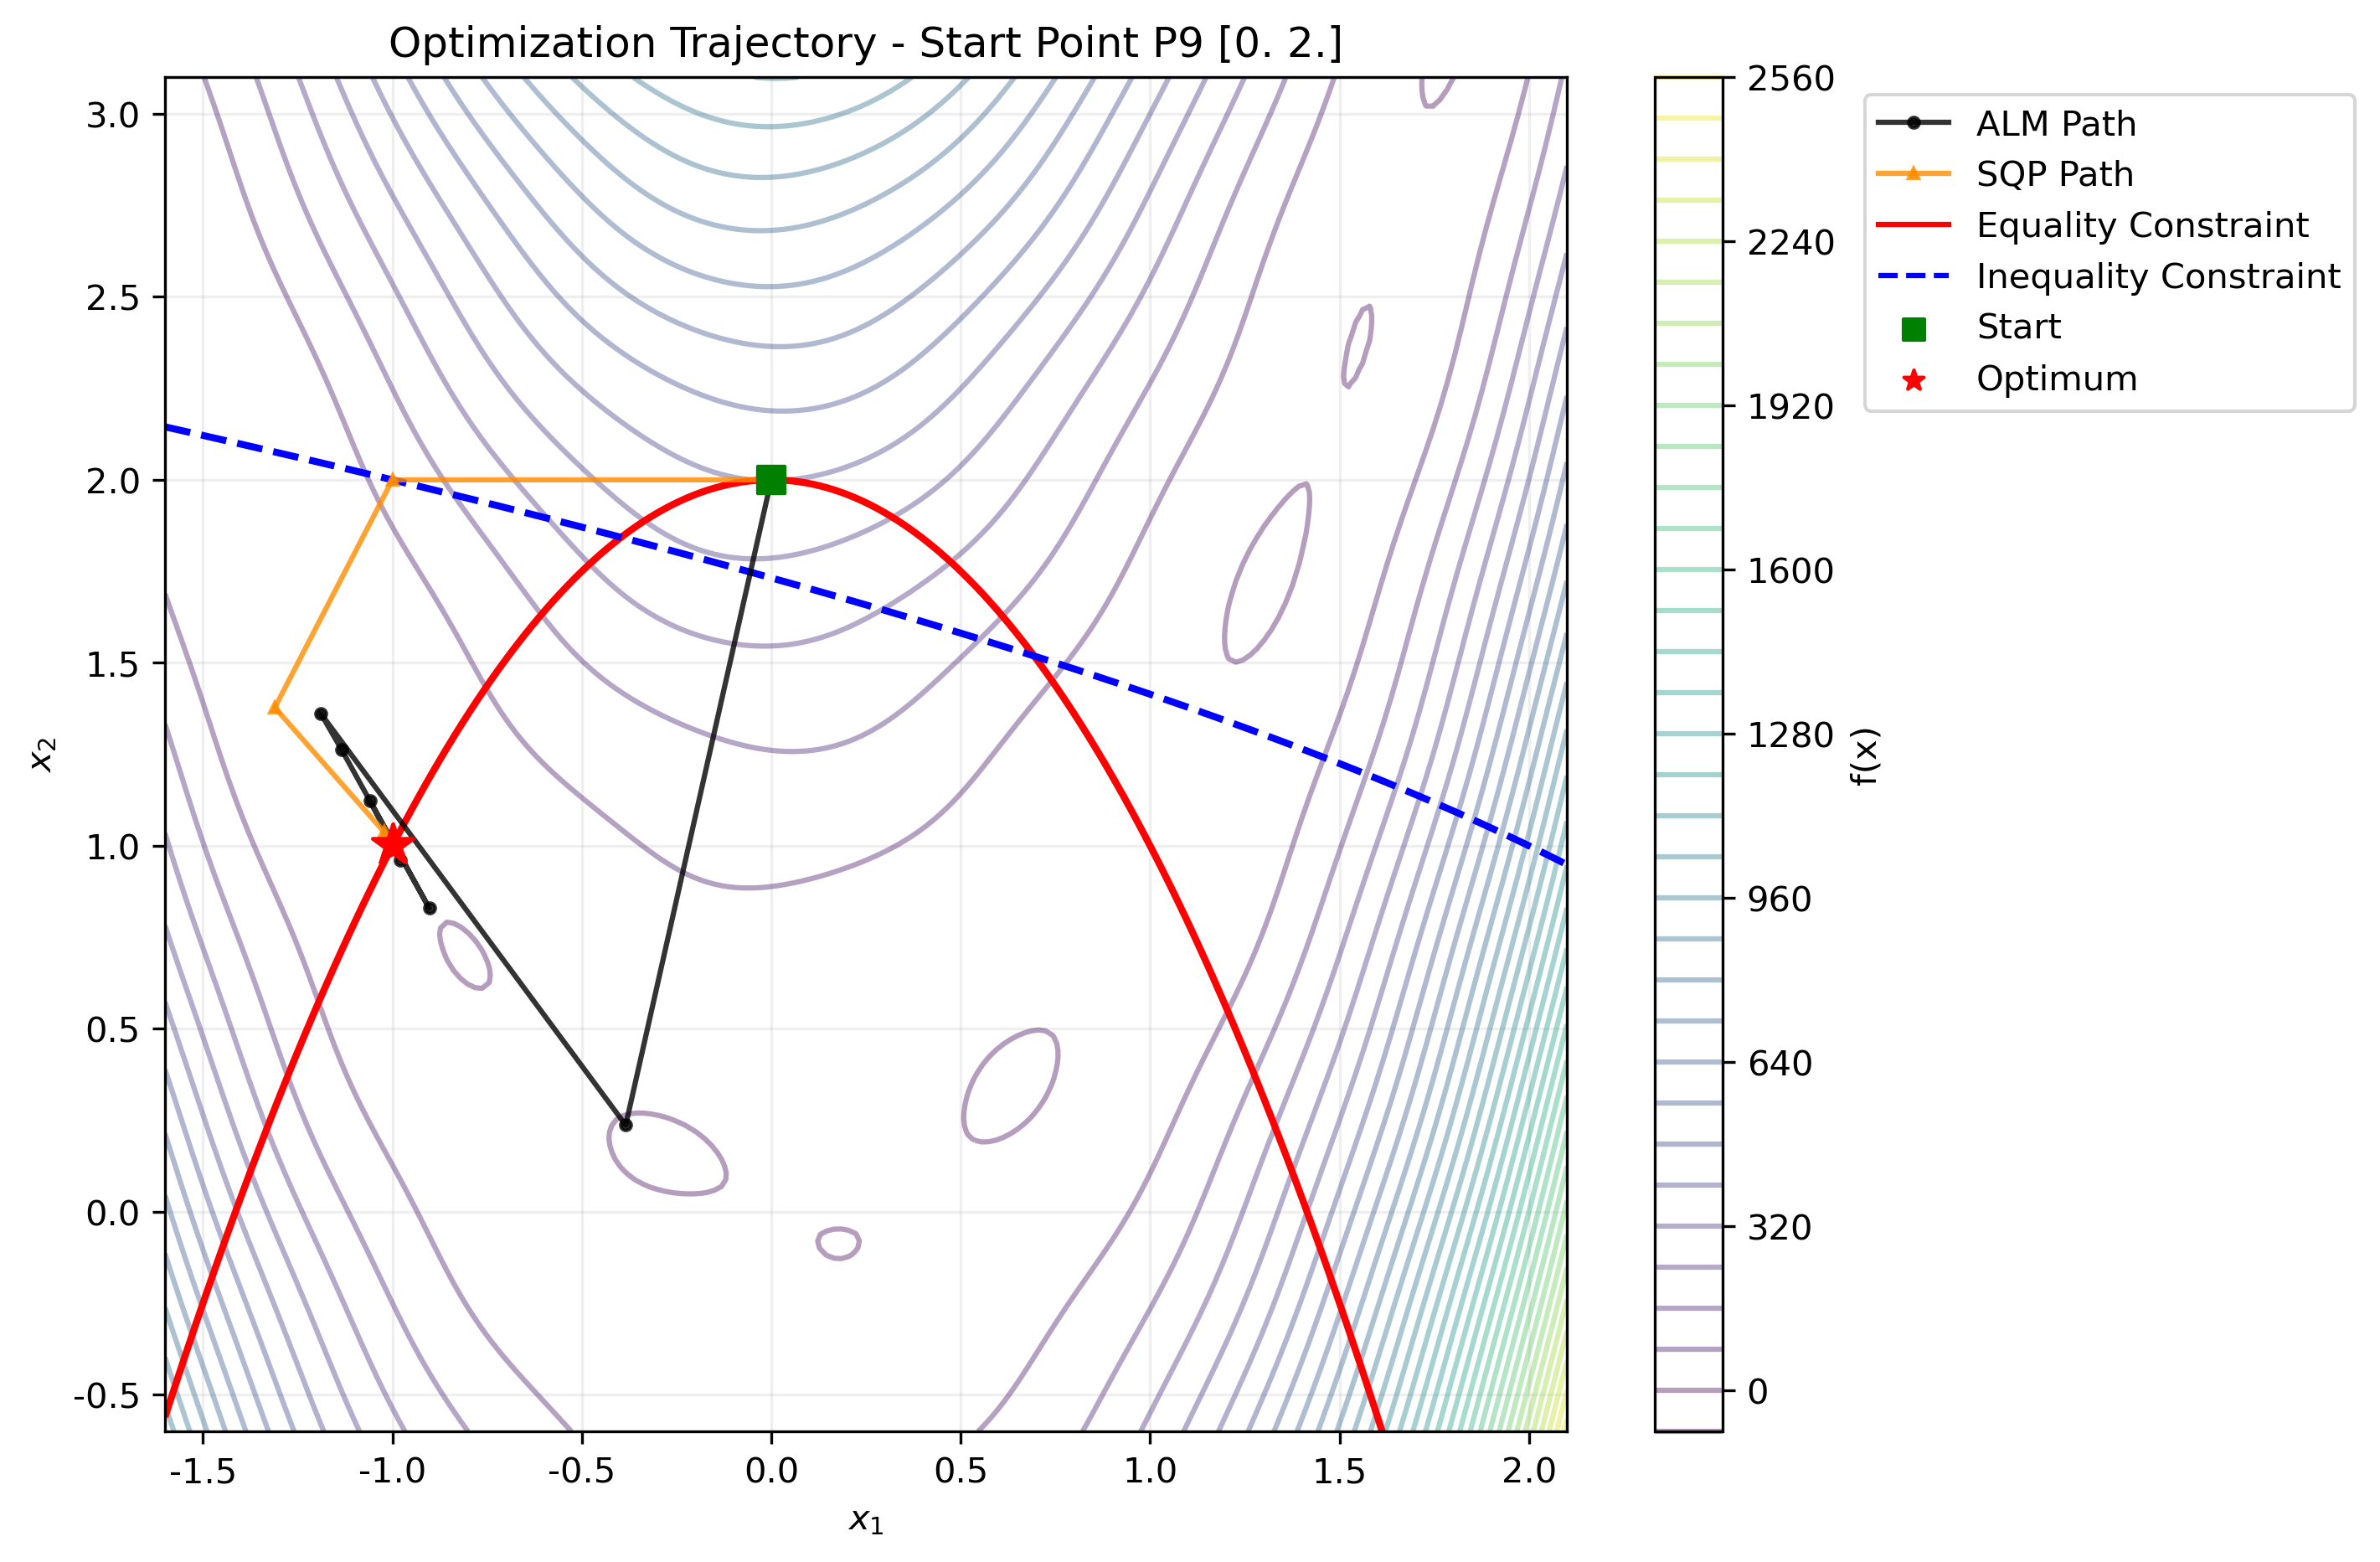
\includegraphics[width=\textwidth]{figures/path_2D_P9.png} \caption{$P_9$}
    \end{subfigure}
    \hfill
    \begin{subfigure}[b]{0.48\textwidth}
        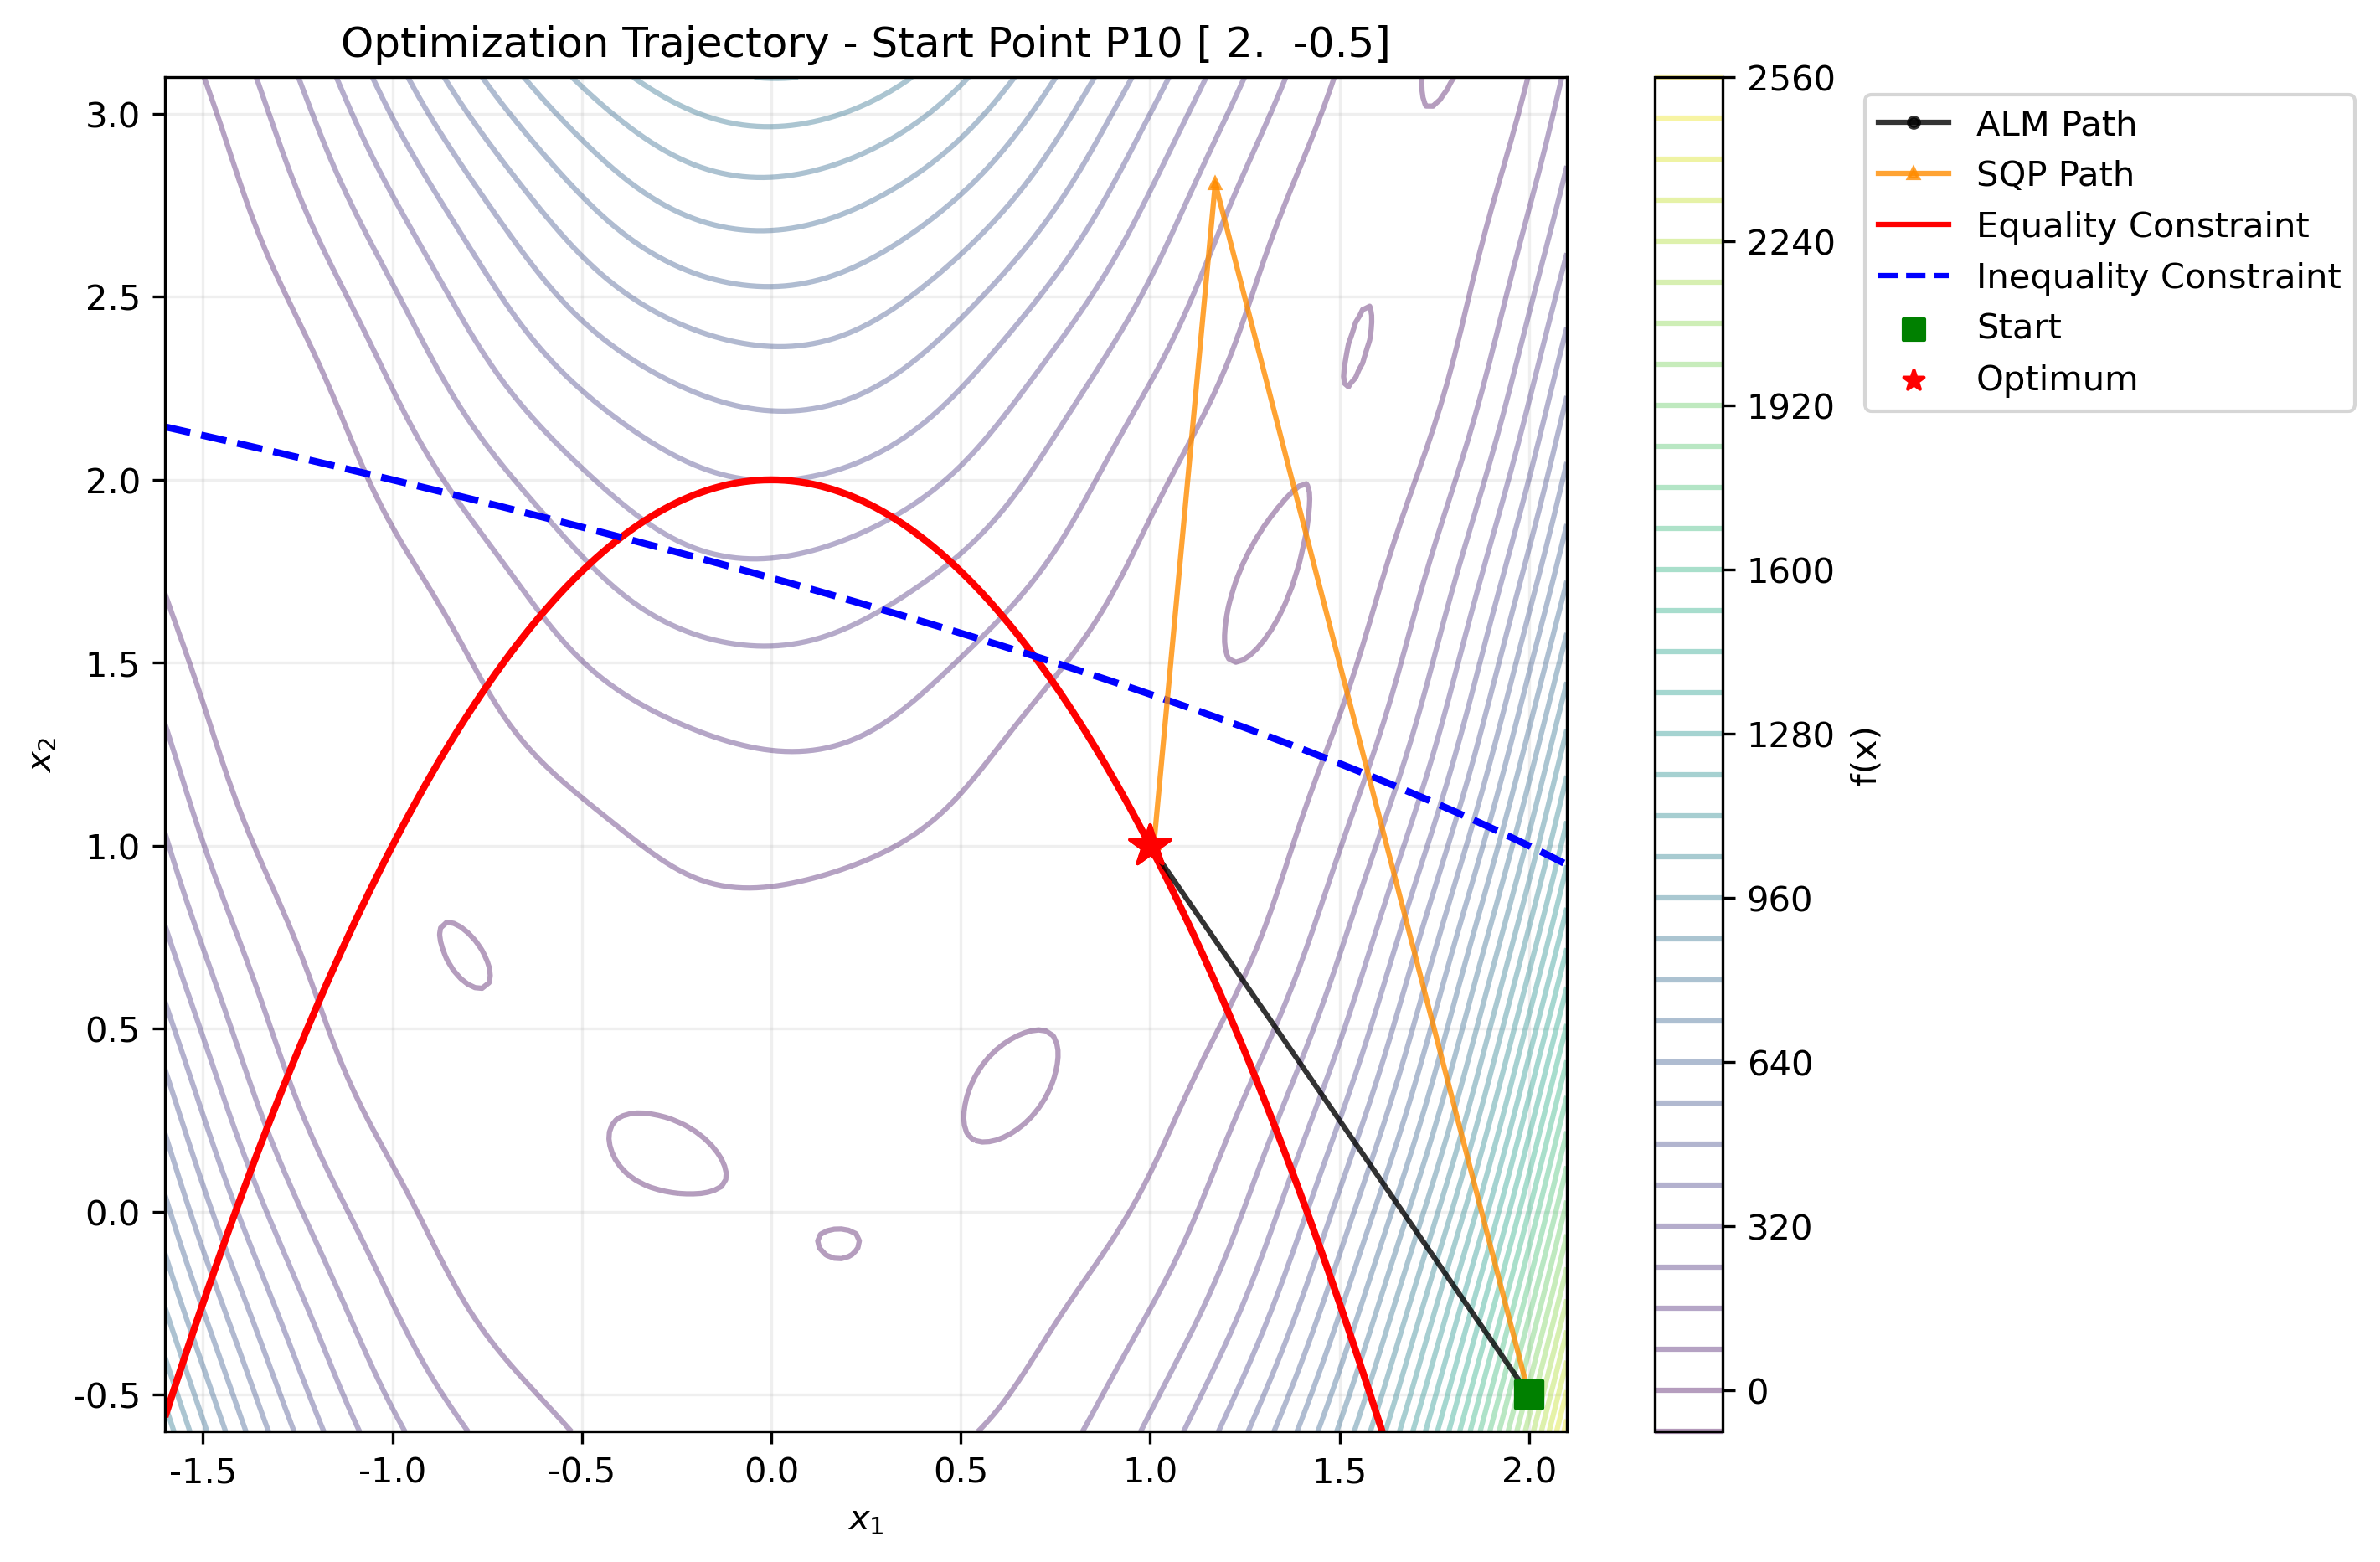
\includegraphics[width=\textwidth]{figures/path_2D_P10.png} \caption{$P_{10}$}
    \end{subfigure}
    
    % 续标题
    \caption[]{2D Modified Rosenbrock 问题迭代轨迹对比（续）。}
\end{figure}

\clearpage
\subsection{4D 问题可视化分析}

对于高维约束问题，图 \ref{fig:app_summary_4d} 和图 \ref{fig:app_conv_grid_4d} 分别展示了算法的计算开销与收敛稳定性。

% --- 4. 4D 概览图 ---
\begin{figure}[hbt!]
    \centering
    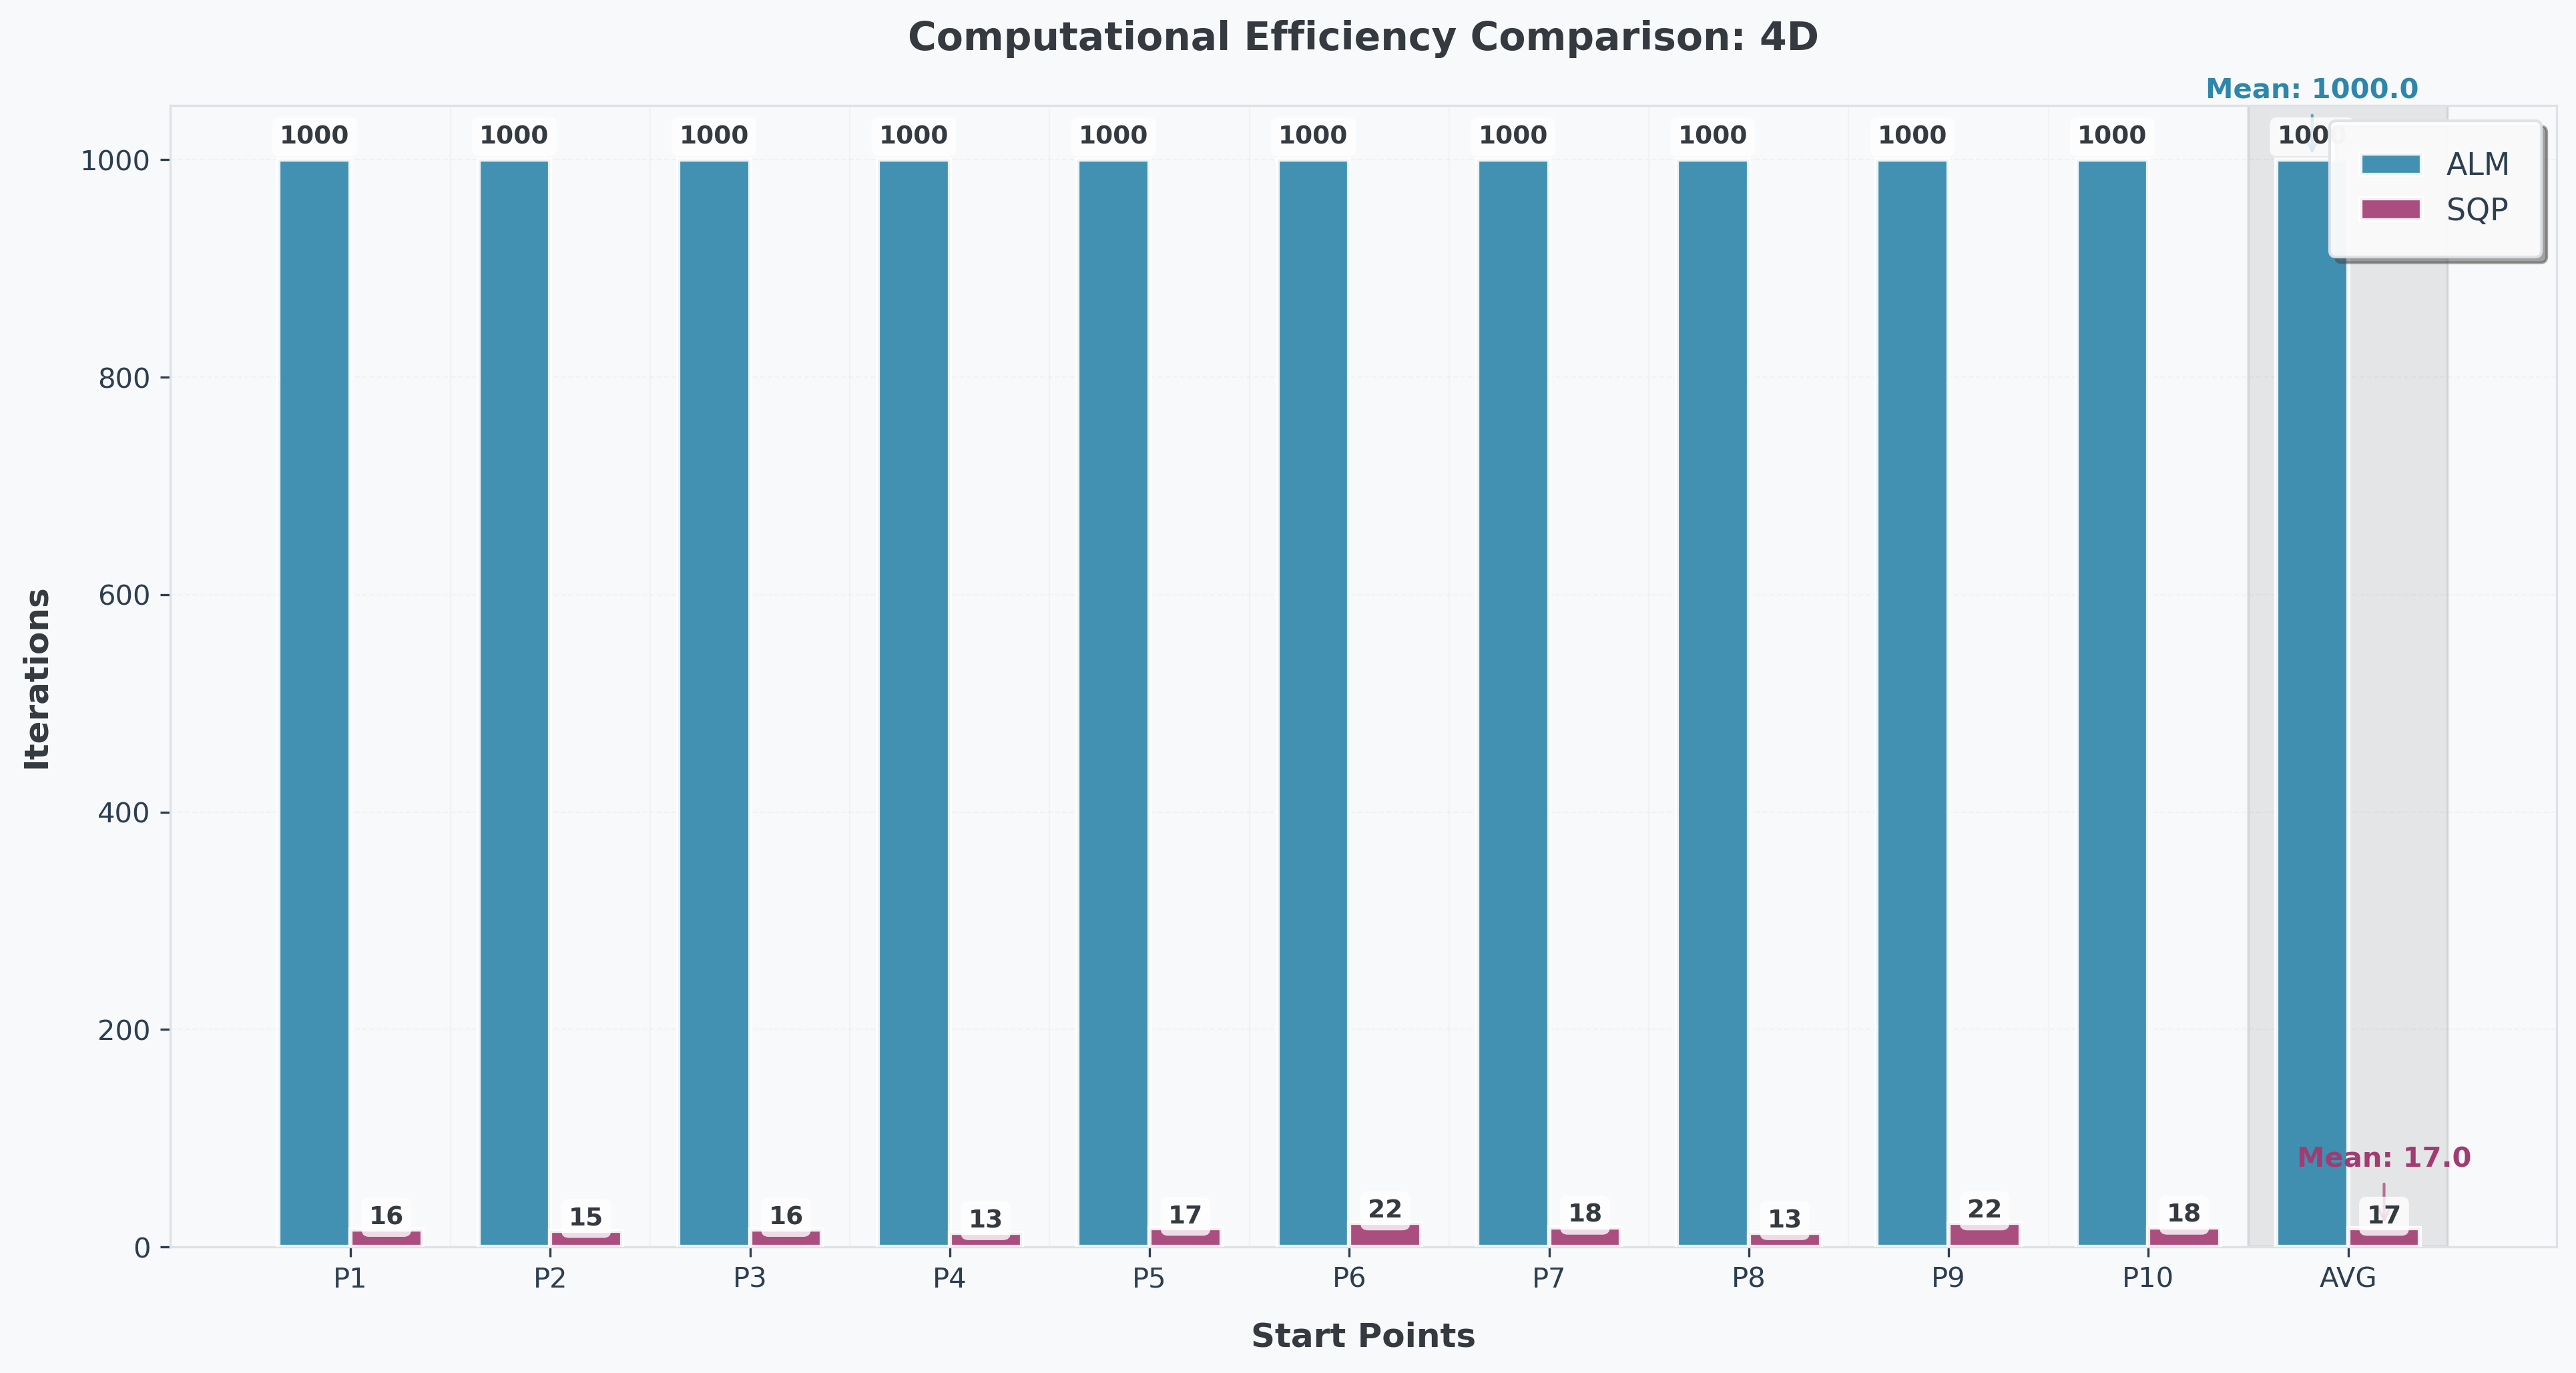
\includegraphics[width=0.9\textwidth]{figures/summary_4D.png}
    \caption{4D 测试问题：不同初始点下的迭代次数 (Iterations) 对比统计}
    \label{fig:app_summary_4d}
\end{figure}

% --- 5. 4D 收敛曲线网格图 ---
\begin{figure}[hbt!]
    \centering
    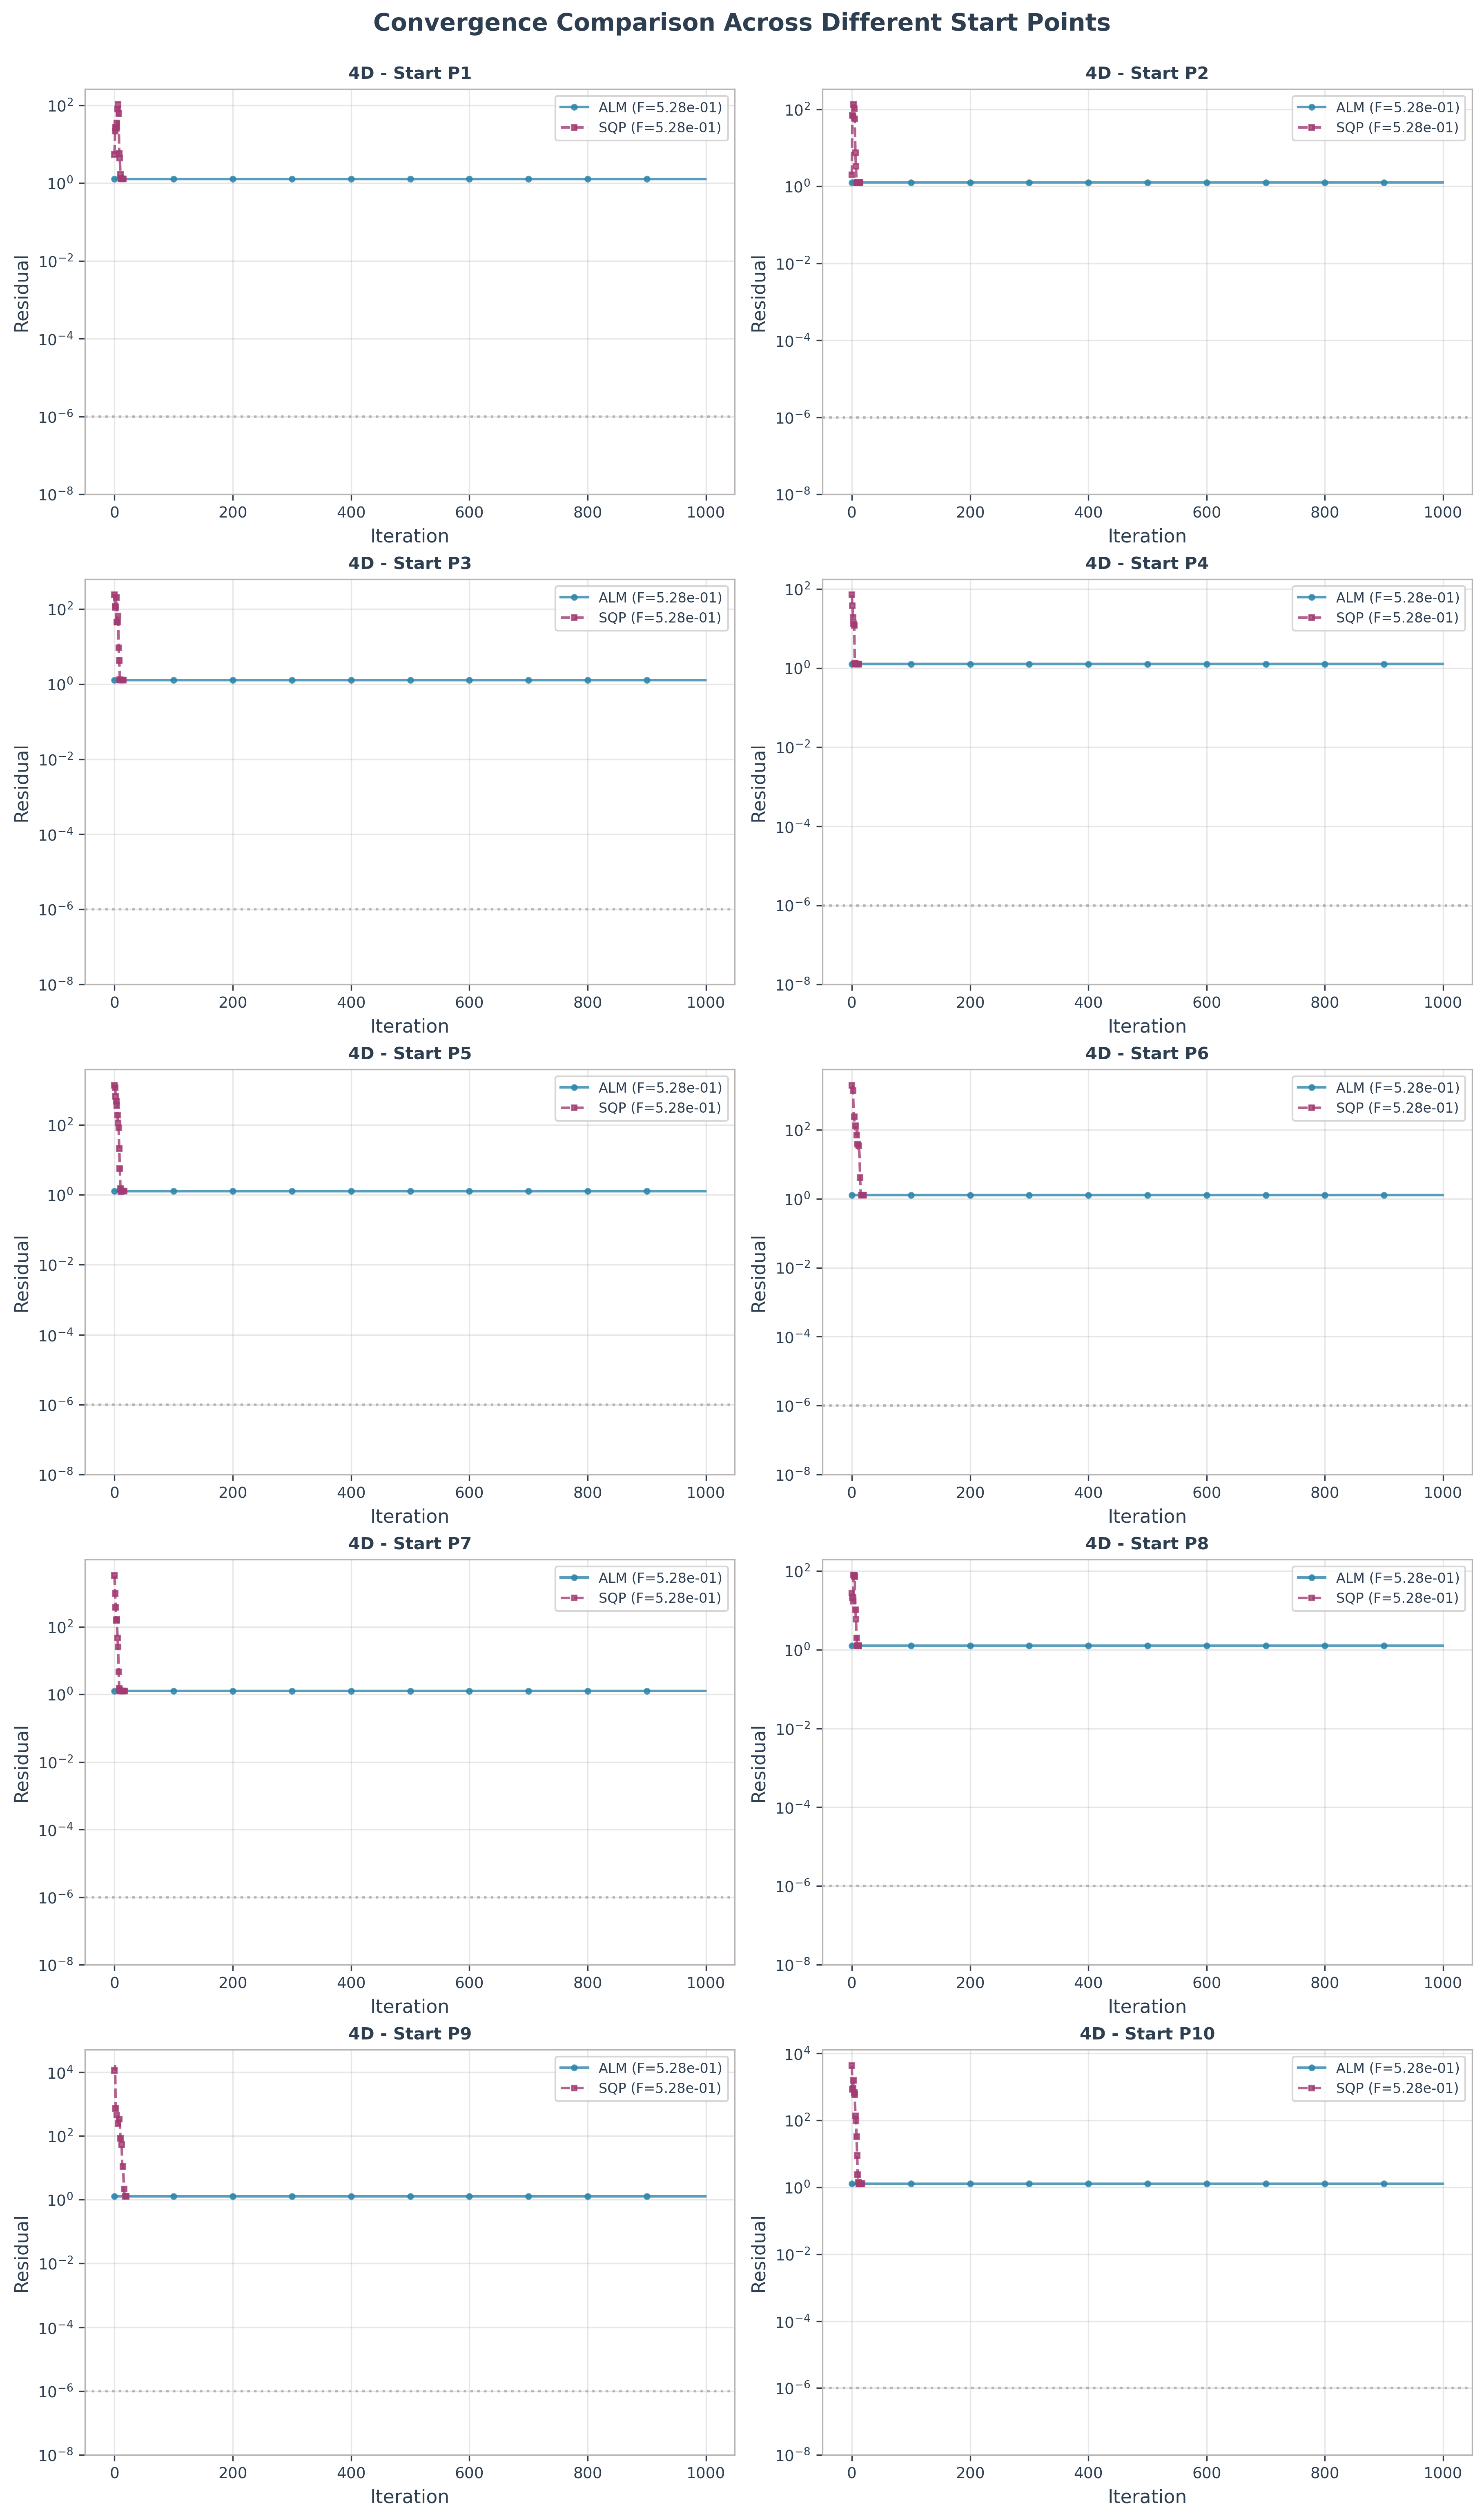
\includegraphics[width=1.0\textwidth, height=0.9\textheight, keepaspectratio]{figures/convergence_grid_comparison_4D.png}
    \caption{4D 测试问题：所有初始点的 KKT 误差收敛曲线网格图。SQP 均表现出超线性收敛特征。}
    \label{fig:app_conv_grid_4d}
\end{figure}
\clearpage

\section{优化算法 Python 实现} \label{app:code}

以下是本研究中使用的核心优化算法代码：

% --- 方式 A: 直接在 tex 文件中写代码 ---
% \begin{lstlisting}[caption={SQP 算法实现}, label={code:sqp}]
% import numpy as np

% def objective_function(x):
%     """
%     计算目标函数值
%     """
%     return x[0]**2 + x[1]**2

% def main():
%     x_start = np.array([1.0, 1.0])
%     print("Optimization Started")
%     # 迭代过程...
%     return 0
% \end{lstlisting}

% --- 方式 B: 从外部文件导入 (推荐用于长代码) ---
% 假设你有一个名为 solver.py 的文件在同一目录下
% \lstinputlisting[language=Python, caption={主程序源码}]{run.py}

% \lstinputlisting[language=Python, caption={求解器源码}]{solver.py}

% \lstinputlisting[language=Python, caption={绘图代码}]{plot_utils.py}

% 这里通过命令批量导入，非常整洁
\includepy{主程序 (run.py)}{codes/run.py}
\includepy{优化算法 (solver.py)}{codes/solver.py}
% 下面这一行改了：在 plot 和 util 之间加反斜杠
\includepy{辅助工具 (plot\_utils.py)}{codes/plot_utils.py}




\end{document}